%% LyX 2.1.4 created this file.  For more info, see http://www.lyx.org/.
%% Do not edit unless you really know what you are doing.
\documentclass[a4paper,oneside,brazil,11pt,a4paper,openright,titlepage,usenames,dvipsnames]{book}
\usepackage[utf8]{inputenc}
\usepackage[T1]{fontenc}
\usepackage{lmodern}
\setcounter{secnumdepth}{3}
\setcounter{tocdepth}{3}
\usepackage{array}
\usepackage{verbatim}
\usepackage{calc}
\usepackage{textcomp}
\usepackage{amssymb}
\usepackage{graphicx}

\makeatletter

%%%%%%%%%%%%%%%%%%%%%%%%%%%%%% LyX specific LaTeX commands.
\pdfpageheight\paperheight
\pdfpagewidth\paperwidth

%% Because html converters don't know tabularnewline
\providecommand{\tabularnewline}{\\}

%%%%%%%%%%%%%%%%%%%%%%%%%%%%%% User specified LaTeX commands.
% Classe alternativa, apropriada para impressão frente-verso. Inclui páginas em branco
% de forma que capítulos sempre tenham início na página à direita:
% \documentclass[11pt,a4paper,openright,titlepage]{book}

% Pacotes
\usepackage[T1]{fontenc}
\usepackage[brazilian]{babel}
\usepackage{epsfig}
\usepackage{subfig}%\usepackage{subfigure}
\usepackage{floatrow}
\usepackage{amsfonts}
\usepackage{amsmath}
\usepackage[thmmarks,amsmath]{ntheorem}%\usepackage{amsthm}
\usepackage{boxedminipage}
\usepackage{geometry}
\usepackage{theorem}
\usepackage{fancybox}
\usepackage{fancyhdr}
\usepackage{ifthen}
\usepackage{url}
\usepackage{afterpage}
\usepackage{color}
\usepackage{colortbl}
\usepackage{rotating}
\usepackage{makeidx}
\usepackage{indentfirst}
% Pacotes para adição de figuras do inkscape
\usepackage{graphicx}
\usepackage{import}

% Escolher um dos seguintes formatos:
\usepackage{template-FT-UnB/ft2unb} % segue padrão de fontes do Latex

% Extras:
\usepackage{quoting}
\usepackage{multicol}
\usepackage{lscape}

\makeindex

\makeatother

\usepackage{babel}
\begin{document}
\setcounter{secnumdepth}{3}
\setcounter{tocdepth}{2}
\pagestyle{empty}

\grau{Engenheiro de Controle e Automação}

\tipodemonografia{ADENDO AO TRABALHO DE GRADUAÇÃO}

\begin{comment}
Título
\end{comment}


\titulolinhai{ESCLARECIMENTO ACERCA DO MODELO PROPOSTO}

\titulolinhaii{DENAVIT-HARTENBERG}

\titulolinhaiii{}

\titulolinhaiv{}

\begin{comment}
Autores. Basta retirar o texto totalmente caso não haja um determinado
autor.
\end{comment}

\autori{Rafael Augusto Torres}

\autorii{}

\autoriii{}

\begin{comment}
Membros da banca. Basta retirar o texto totalmente caso não haja um
determinado membro da banca.
\end{comment}

\membrodabancai{Prof. Walter de Britto Vidal Filho, ENM/UnB}

\membrodabancaifuncao{Orientador}

\membrodabancaii{Prof. Guilherme Caribé de Carvalho, ENM/UnB}

\membrodabancaiifuncao{Examinador interno}

\membrodabancaiii{Prof. José Maurício Santos Torres da Motta, ENM/UnB}

\membrodabancaiiifuncao{Examinador interno}

\membrodabancaiv{}

\membrodabancaivfuncao{}

\membrodabancav{}

\membrodabancavfuncao{}

\begin{comment}
Data de defesa: mês e ano
\end{comment}

\mes{dezembro}
\ano{2020}

\begin{comment}
Comandos para criar a capa e a página de assinaturas
\end{comment}

\capaprincipal
%\capaassinaturas

\begin{comment}
Ficha Catalográfica
\end{comment}

%\noindent \textbf{FICHA CATALOGRÁFICA}

\noindent %
\fbox{\begin{minipage}[t]{1\columnwidth}%
TORRES, RAFAEL AUGUSTO

Instrumentação e Controle de Braço Robótico para Deficientes / Rafael Augusto Torres; orientador Walter de Britto Vidal Filho. 

\medskip{}


{[}Distrito Federal{]} 2020.

\medskip{}


xiv, 96p., 297 mm (FT/UnB, Engenheiro, Controle e Automação, 2020).
Trabalho de Graduação \textendash{} Universidade de Brasília. Faculdade
de Tecnologia.

\medskip{}


1. Braço Robótico Montado Sobre Cadeira de Rodas \hfill{}2.Tecnologias Assistivas\hfill{}

3. Sensoriamento Robótico

\medskip{}


I. Mecatrônica/FT/UnB\hfill{}II. Título (Série)\hfill{}

%
\end{minipage}}

\noindent \medskip{}


\noindent \textbf{REFERÊNCIA BIBLIOGRÁFICA}

TORRES, R. A., (2020). Instrumentação e Controle de Braço Robótico para Deficientes. Trabalho de Graduação
em Engenharia de Controle e Automação, Publicação FT. TG-$n^{\circ}022$,
Faculdade de Tecnologia, Universidade de Brasília, Brasília, DF, 96p.

\noindent \bigskip{}


\noindent \textbf{CESSÃO DE DIREITOS}

\noindent AUTOR: Rafael Augusto Torres

TÍTULO DO TRABALHO DE GRADUAÇÃO: Instrumentação e Controle de Braço Robótico para Deficientes.

\noindent \medskip{}


\noindent GRAU: Engenheiro\hfill{}ANO: 2020\hfill{}

\noindent \medskip{}


É concedida à Universidade de Brasília permissão para reproduzir cópias
deste Trabalho de Graduação e para emprestar ou vender tais cópias
somente para propósitos acadêmicos e científicos. O autor reserva
outros direitos de publicação e nenhuma parte desse Trabalho de Graduação
pode ser reproduzida sem autorização por escrito do autor.

\noindent \bigskip{}


\noindent \rule[0.5ex]{1\columnwidth}{1pt}

\noindent Rafael Augusto Torres

\noindent Campus Darcy Ribeiro, ULEG, Universidade de Brasília.

\noindent 70910-900 Brasília \textendash{} DF \textendash{} Brasil.


\begin{comment}
Dedicatória
\end{comment}

\frontmatter

\begin{comment}
Texto de dedicatória do primeiro autor.
\end{comment}

\dedicatoriaautori{Dedicatória!}

\begin{comment}
Texto de dedicatória do segundo autor. Caso não tenha um segundo autor,
este texto não será mostrado
\end{comment}

\dedicatoriaautorii{Dedicatória do autor 2}

\begin{comment}
Texto de dedicatória do terceiro autor. Caso não tenha um terceiro
autor, este texto não será mostrado
\end{comment}

\dedicatoriaautoriii{Dedicatória do autor 3}

\begin{comment}
Comando para criar a página de dedicatória
\end{comment}

%\dedicatoria

\begin{comment}
Agradecimentos
\end{comment}


\begin{comment}
Texto de agradecimentos do primeiro autor.
\end{comment}


\agradecimentosautori{Obrigado!}

\begin{comment}
Texto de agradecimentos do segundo autor. Caso não tenha um segundo
autor, este texto não será mostrado.
\end{comment}


\agradecimentosautorii{A inclusão desta seção de agradecimentos é
opcional e fica à critério do(s) autor(es), que caso deseje(em) inclui-la
deverá(ão) utilizar este espaço, seguindo esta formatação.}

\begin{comment}
Texto de agradecimentos do terceiro autor. Caso não tenha um terceiro
autor, este texto não será mostrado.
\end{comment}


\agradecimentosautoriii{A inclusão desta seção de agradecimentos
é opcional e fica à critério do(s) autor(es), que caso deseje(em)
inclui-la deverá(ão) utilizar este espaço, seguindo esta formatação.}

\begin{comment}
Comando para criar a página de agradecimentos
\end{comment}

% Inicia caption das tables no topo
\floatsetup[table]{capposition=top}

%\agradecimentos

%\resumo{resumo}{
%
%Este trabalho tem como finalidade apresentar o projeto de circuitos de instrumentação e acionamento, bem como de um sistema 
%central, para controle de um braço robótico montado em uma cadeira de rodas, a ser utilizado por pessoas com deficiências motoras.
%O projeto de circuitos conta com a escolha de todos os dispositivos relacionados a serem inseridos na estrutura do manipulador,
%visando garantir uma boa integridade dos sinais transmistidos e boa resposta de atuação.
%Os circuitos de acionamento, processamento e controle são em sua totalidade baseados em modelos comerciais, que já
%possuem uma grande confiabilidade e baixo custo no mercado.
%O sistema de controle do robô foi desenvolvido de modo a transformar velocidades informadas por um usuário através de um \textit{joystick}
%em velocidades a serem impostas nas juntas, controlando simultanemante todos os atuadores do sistema.
%Foi criado um ambiente de simulação para facilitar a visualização da posição e orientação do manipulador. O ambiente realiza
%uma animação do robô na tela com base em dados obtidos pelo microcontrolador empregado, e, através deste, foi possível 
%validar o funcionamento dos circuitos e do sistema de controle propostos.
%
%\medskip{}
%
%Palavras Chave: Braço Robótico Montado Sobre Cadeira de Rodas, Tecnologias Assistivas, Manipulador Robótico, Sensoriamento Robótico.
%
%}\vspace*{2cm}
%
%\newpage
%
%\resumo{Abstract}{
%
%This work has as purpose the presentation of instrumentation and driver circuits design, as well as the design of a central system, for
%controlling a weelchair mounter robotic arm, to be used by people with motor impairments.
%The circuits design takes in consideration the choice of all the related devices to be inserted in the manipulator structure,
%aiming to guarantee a good signal integrity for the transmitted signals and a good actuation response.
%The driver, processing and control circuits are entirely based on commercial models, which already show a great reliability and
%low cost in the market.
%The robot's control system was developed in a way to transform speeds informed by the user through a joystick into speeds to be
%imposed on the joints, controlling all the system's motors simultaneously.
%A simulation environment was created to facilitate the visualization of the manipulator position and orientation. The environment
%performs the robot's animation based on data obtained by the microcontroller employed, and, through this mean, it was possible
%to validate the proposed circuits and control system operations.
%
%\medskip{}
%
%
%Keywords: Wheelchair Mounted Robotic Arm, Assitive Technologies, Robotic Manipulator, Robot Sensing.
%
%}

\begin{comment}
Listas de conteúdo, figuras e tabelas
\end{comment}


\sumario
\listadefiguras
%\listadetabelas

\begin{comment}
Lista de Símbolos
\end{comment}

%%TCIDATA{LaTeXparent=0,0,these.tex}


%\chapter*{\setfontarial\mdseries LISTA DE SÍMBOLOS} % se usar ft1unb.sty, descomente esta linha



\chapter*{LISTA DE SÍMBOLOS}

% se usar ft2unb.sty, descomente esta linha



\subsection*{Símbolos Latinos}

\begin{tabular}{p{0.1\textwidth}p{0.63\textwidth}>{\PreserveBacklash\raggedleft}p{0.15\textwidth}}
$e$             & Força contra-eletromotriz     & {[}V{]}           \tabularnewline    
$I$             & Corrente elétrica             & {[}A{]}           \tabularnewline 
$\mathcal{I}$   & Momento de inércia angular    & {[}kg.m$^2${]}    \tabularnewline
$J$             & Matriz Jacobiana              &                   \tabularnewline
$M$             & Torque/Momento de de Força    & {[}N.m{]}         \tabularnewline
$r$             & Vetor de posição              & {[}3x1m{]}        \tabularnewline
$t$             & Tempo                         & {[}s{]}           \tabularnewline
$T$             & Matriz de transformação       &                   \tabularnewline
$v$             & Velocidade linear             & {[}m/s{]}         \tabularnewline
$V$             & Tensão elétrica               & {[}V{]}           \tabularnewline
$Z$             & Impedância elétrica           & {[}$\Omega${]}    \tabularnewline 
\end{tabular}


\subsection*{Símbolos Gregos}

\begin{tabular}{p{0.1\textwidth}p{0.63\textwidth}>{\PreserveBacklash\raggedleft}p{0.15\textwidth}}
$\alpha$    & Ângulo, constante         & {[}rad{]}     \tabularnewline
$\delta$    & Variação                  &               \tabularnewline
$\theta$    & Ângulo, variável          & {[}rad{]}     \tabularnewline
$\Theta$    & Vetor de ângulos          &               \tabularnewline
$\tau$      & Constante de tempo        & {[}s{]}       \tabularnewline
$\omega$    & Velocidade angular        & {[}rad/s{]}   \tabularnewline
$\nu$       & Vetor de velocidades      &               \tabularnewline
\end{tabular}


\subsection*{Grupos Adimensionais}

\begin{tabular}{p{0.1\textwidth}p{0.8\textwidth}}
i, k    &   Contador    \tabularnewline
\end{tabular}


\subsection*{Subscritos}

\begin{tabular}{p{0.1\textwidth}p{0.8\textwidth}}
$Th$    & Equivalente de Thévenin   \tabularnewline
%$ref$  & referência \tabularnewline
%$fer$  & ferramenta \tabularnewline
%$sis$  & sistema \tabularnewline
%$des$  & desejado\tabularnewline
\end{tabular}


\subsection*{Sobrescritos}

\begin{tabular}{p{0.1\textwidth}p{0.8\textwidth}}
$\hat{}$    & Vetor unitário    \tabularnewline
$\cdot$     & Variação temporal \tabularnewline7
%$-$  & Valor médio \tabularnewline
\end{tabular}


\subsection*{Siglas}

\begin{tabular}{p{0.1\textwidth}p{0.8\textwidth}}
ABS     & \textit{Acrylonitrile Butadiene Styrene} - Acrilonitrila Butadieno Estireno           \tabularnewline   
AC      & \textit{Alternating Current} - Corrente Alternada                                     \tabularnewline
ADC     & \textit{Analog-to-Digital Converter} - Conversor Analógico-Digital                    \tabularnewline
ADL     & \textit{Activities of Daily Living} - Atividades Diárias Básicas                      \tabularnewline
CI      & Circuito Integrado                                                                    \tabularnewline
CMRR    & \textit{Common-Mode Rejection Ratio} - Taxa de Rejeição de Modo Comum                 \tabularnewline
CTR     & \textit{Current Transfer Ratio} - Taxa de Transmissão de Corrente                     \tabularnewline
DC      & \textit{Direct Current} - Corrente Contínua                                           \tabularnewline
DH      & Denavit-Hartenberg                                                                    \tabularnewline
LED     & \textit{Light Emitting Diode} - Diodo Emissor de Luz                                  \tabularnewline
MCU     & \textit{Microcontroller Unit} - Unidade microcontroladora                             \tabularnewline
ONU     & Organização das Nações Unidas                                                         \tabularnewline
PIC     & \textit{Peripheral Interface Controller} - Controlador de Interface Periférica        \tabularnewline
PID     & Proporcional Integral Derivativo                                                      \tabularnewline
PLA     & Poliácido láctico                                                                     \tabularnewline
PPR     & Pulsos por revolução                                                                  \tabularnewline
PVC     & \textit{Polyvinyl chloride} - Policloreto de vinila                                   \tabularnewline
PWM     & \textit{Pulse Width Modulation} - Modulação por largura de pulso                      \tabularnewline
TA      & Tecnologia Assistiva                                                                  \tabularnewline
UnB     & Universidade de Brasília                                                              \tabularnewline
WMRA    & \textit{Weelchair Mounted Robotic Arm} - Braço Robótico Montado em Cadeira de Rodas   \tabularnewline
%PCI  & \textit{Peripheral Component Interconnect}\tabularnewline
%CPU & Unidade Central de Processamento - \textit{Central Processing Unit} \tabularnewline
%AO & Saída Analógica - \textit{Analog Out}\tabularnewline
%DO & Saída Digital - \textit{Digital Out}\tabularnewline
%CS & Seletor de \textit{Chip - Chip Select}\tabularnewline
%SC & Sem Conexão\tabularnewline
%P.I. & Placa de Interface\tabularnewline
%ICW & \textit{Initialization Command Words}\tabularnewline
%OCW & \textit{Operational Control Word}\tabularnewline
\end{tabular}


\begin{comment}
Corpo Principal
\end{comment}

\mainmatter
\setcounter{page}{1}
\pagenumbering{arabic}
\pagestyle{plain}

%\begin{comment}
%Temp
%\end{comment}
%\chapter{A ORGANIZAR}

\section{Cinemática Inversa}
Além do controle por velocidade do manipulador, utilizando a jacobiana inversa
para transformar comandos de velocidade desejada pelo usuário em velocidades das juntas, é possível controlar 
o braço robótico também por meio de inserção da posição e orientação desejadas, transformando
essas informações em valores das juntas por meio da cinemática inversa.

Inicialmente, assume-se que o usuário irá informar a posição e orientação da ferramenta em uso pelo
manipulador, ou do efetuador final, em relação ao sistema de coordenadas da estação. Esta relação entre 
sistema de coordenadas da ferramenta e estação pode ser transformado em uma relação 
entre os sistemas de coordenadas da última junta do manipulador em relação à primeira, da seguinte forma:

\begin{equation*}
    ^B_WT = ^B_S\!T\;^S_TT\;^W_TT^{-1}
\end{equation*}

A relação entre o punho, representado pelo \{$W$\}, do inglês \textit{wrist}, e a base \{B\},
é dada por:

\begin{equation*}
    ^B_WT = \; ^0_6T = 
    \begin{bmatrix}
        r_{11} & r_{12} & r_{13} & p_x \\
        r_{21} & r_{22} & r_{23} & p_y \\
        r_{31} & r_{32} & r_{33} & p_z \\
           0   &    0   &    0   &  1  \\    
    \end{bmatrix}
\end{equation*}

Para obter uma relação mais simples da geometria do robô é interessante ter uma relação 
entre a junta 5 a junta 1, portante, tanto a matriz acima quanto a matriz da equação \ref{eq:0T6}
serão multiplicadas por $^0_1T^{-1}$ e $^5_6T^{-1}$ na seguinte ordem:

\begin{equation*}
    ^1_5T = ^0_1\!T^{-1}\;^0_6T\;^5_6T^{-1}
\end{equation*}

Realizando esta transformação para a matriz que possui como parâmetros os ângulos das juntas
é obtido o seguinte resultado:

\begin{equation*}
    ^1_5T = 
    \begin{bmatrix}
        s_5c(\Theta) & c_5c(\Theta) & s(\Theta) & c(\Theta)a_5 + c(\theta_2+\theta_3)a_4 + c_2a_3 + a_2 \\
        c_5 & -s_5 & 0 & -(d_3+d_4) \\
        s_5s(\Theta) & c_5s(\Theta) & -c(\Theta) & s(\Theta)a_5+s(\theta_2+\theta_3)a_4 + s_2a_3 \\
           0   &    0   &    0   &  1  \\    
    \end{bmatrix}
\end{equation*}

onde,

\begin{equation*}
    \Theta = \theta_2+\theta_3+\theta_4
\end{equation*}

Agora, para a matriz $^0_6T$ com base nos parâmetros desejados, o obtido é:

\begin{equation*}
    ^1_5T = 
    \begin{bmatrix}
         c_1(r_{11}c_6-r_{12}s_6) &  c_1r_{13}+s_1r_{23} & -c_1(r_{11}s_6+r_{12}c_6) &  c_1(p_x-r_{13}d_6) \\
        +s_1(r_{21}c_6-r_{22}s_6) &                      & -s_1(r_{21}s_6+r_{22}c_6) & +s_1(p_y-r_{23}d_6) \\
        & & & & \\
        -s_1(r_{11}c_6-r_{12}s_6) & -s_1r_{13}+c_1r_{23} &  s_1(r_{11}s_6+r_{12}c_6) & -s_1(p_x-r_{13}d_6) \\
        +c_1(r_{21}c_6-r_{22}s_6) &                      & -c_1(r_{21}s_6+r_{22}c_6) & +c_1(p_y-r_{23}d_6) \\
        & & & & \\        
             r_{31}c_6-r_{32}s_6  &         r_{33}       &     -r_{31}s_6-r_{32}c_6  &      p_z-r_{33}d_6  \\
        & & & & \\
                    0             &            0         &              0            &           1         \\    
    \end{bmatrix}
\end{equation*}

Os termos $p_x-r_{13}d_6$ e $p_y-r_{23}d_6$ equivalem, respectivamente, às posições x e y da quinta junta no sistema 
de coordenadas da primeira junta, assim, alternando esses termos para suas respectivas coordenadas polares,
obtém-se:

\begin{align*}
    p_x - r_{13}d_6 &= \; ^1_5\rho_x = \; ^1_5\rho \cdot cos ^1_5\phi \\
    p_y - r_{23}d_6 &= \; ^1_5\rho_y = \; ^1_5\rho \cdot sen ^1_5\phi \\
\end{align*}

Substituindo os valores mais a direita no termo (2, 4) da matriz e igualando ao termo (2, 4) da matriz em função
das variáveis das juntas, chega-se à seguinte relação:

\begin{equation*}
    -s_1 \cdot ^1_5\rho \cdot cos ^1_5\phi + c_1 \cdot ^1_5\rho \cdot sen ^1_5\phi = - (d_3 + d_4)
\end{equation*}

, assim:

\begin{equation*}
    sen(\theta_1 - ^1_5\phi) = \frac{d_3+d_4}{^1_5\rho}
\end{equation*}

Utilizando a identidade trigonométrica fundamental, obtém-se também:

\begin{align*}
    cos(\theta_1 - ^1_5\phi) &= \pm \sqrt{1 - \frac{(d_3+d_4)^2}{^1_5\rho^2} } \\
                             &= \pm \frac{\sqrt{^1_5\rho_x^2 + ^1_5\rho_y^2 - (d_3+d_4)^2}}{^1_5\rho}  \\
\end{align*}

Essas duas equações levam ao seguinte resultado para o valor de $\theta_1$:

\begin{align*}
    \theta_1 &= ^1_5\phi + atan2\left(\frac{d_3+d_4}{^1_5\rho}, \frac{\sqrt{^1_5\rho_x^2 + ^1_5\rho_y^2 - (d_3+d_4)^2}}{^1_5\rho}\right) \\
             &= atan2(^1_5\rho_y, ^1_5\rho_x) + atan2\left(d_3+d_4,\sqrt{^1_5\rho_x^2 + ^1_5\rho_y^2 - (d_3+d_4)^2}\right) \\
\end{align*}

\section{others}

\label{A arrumar}
O que está descrito aqui será reescrito e reposicionado melhor no relatório final

% Resumo opcional. Comentar se não usar.
%\resumodocapitulo{Resumo opcional}

\section{Metodologias de projeto}
\label{sec:Fundamentos-Metodologias}

Durante o desenvolvimento de um processo/projeto, são empregadas diferentes ferramentas, abordagens e metodologias para implementar uma gestão da qualidade
deste. A maioria dessas técnicas de gestão são utilizadas em todo o mundo e são simples de entender, no entanto, algumas são mais complexas e demandam um 
maior esforço para serem incluídas no ciclo de vida do processo. É de extrema importância que uma metodologia seja devidamente escolhida e aplicada, 
sendo que o sucesso da sua implementação depende do entendimento e conhecimento acerca desta \cite{sokovic2010quality}.

Vários modelos de metodologias de gestão já foram criadas, com uma gama de aplicações, tanto para o desenvolvimento de \textit{softwares} quanto para o 
desenvolvimento de \textit{hardwares}, como o modelo cascata, espiral, modelo V e ágil. O modelo em cascata é o mais antigo de todos e o mais conhecido,
consistindo de uma sequência de estágios ligados diretamente, onde uma etapa do processo depende da etapa passada. Já o modelo em V demonstra a relação
entre cada fase do ciclo de desenvolvimento e a sua etapa de teste associada. A metodologia ágil surgiu com foco no desenvolvimento de projetos de 
\textit{software}, sendo baseada em iterações e incrementações contínuas, com requisições e soluções evoluindo através da colaboração das equipes
de desenvolvimento \cite{balaji2012waterfall}.

Outros métodos de gestão de qualidade criados propõem uma organização de trabalho mais cíclica, como no caso do ciclo PDCA, ou ciclo de Deming, onde são propostas 4 etapas
que caracterizam o nome desse método: Planejar (\textit{\textbf{P}lan}) - Fazer (\textit{\textbf{D}o}) - Checar (\textit\textbf{C}heck) - Agir (\textit{\textbf{A}ct}).
Este ciclo é considerado como um conceito de melhoria contínua, onde a cada repetição o processo apresenta melhorias em relação ao seu estado original. A metodologia
\textit{Six Sigma} também se baseia em uma melhoria contínua e cíclica do processo. Sendo vista fundamentalmente como uma metodologia para melhoria de processos
já existentes, uma variação do seu ciclo básico foi proposta sob o nome de Projeto para Seis Sigma (DFSS - \textit{Design For Six Sigma}), onde o ciclo de 
trabalho frequentemente é dividido em 5 etapas: Definir (\textit{\textbf{D}efine}) - Medir (\textit{\textbf{M}easure}) - Analisar (\textit{\textbf{A}nalyse}) -
Projetar (\textit{\textbf{D}esign}) - Verificar (\textit{\textbf{V}erify}), sendo este ciclo comumente referido como DMADV \cite{sokovic2010quality}.

\subsection{Cascata}
Como dito anteriormente, o modelo por cascata é um modelo de desenvolvimento sequencial, dada esta natureza, muitas vezes é empregado naturalmente. Neste método
cada passo depende da evolução do passo anterior, sem sobreposição temporal, portanto, é importante que as especificações do projeto sejam bem claras no início
do desenvolvimento, pois estas serão carregadas em todos os passos, assim como ilustrado na figura \ref{fig:Meth-Waterfall}. Dentre os pontos positivos deste 
método estão a alocação temporal específica para cada etapa, facilidade de implementação e a baixa quantidade de ferramentas necessárias para a implementação deste método com sucesso.

No entanto, este método apresenta alguns pontos ruins, como no caso em que há uma mudança nas especificações, esta não estaria prevista no processo de 
desenvolvimento, podendo chegar a não ser implementada. A sequencialidade do método também limita a adequação das etapas a erros, onde um erro pode ocasionar 
o atraso de todas as entregas subsequentes, resultando em um sistema mal estruturado \cite{balaji2012waterfall}. 

\begin{figure}[h]
\caption{Exemplo de fluxo de trabalho por método de cascata}    
\begin{centering}
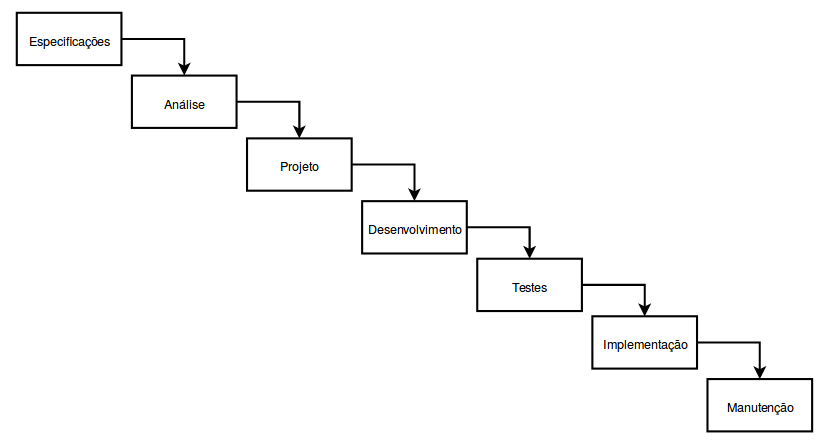
\includegraphics[width=1\columnwidth]{images/meth/Meth-Waterfall.png}
\par\end{centering}

\label{fig:Meth-Waterfall}

\end{figure}

A figura \ref{fig:Meth-Waterfall} exemplifica como a saída de uma etapa é a entrada da seguinte, assim como em uma cascata, evidenciando o nome do método de gestão.

% Falar do Modelo V?

\subsection{Ágil}
Desenvolvido primordialmente para a produção de \textit{softwares}, o manifesto ágil contém vários principios que ditam como deve ser o desenvolvimento de um 
produto, estes princípios prezam pela entrega contínua de código funcional, satisfação do cliente em mente, motivação da equipe e incrementações contínuas 
ao produto \cite{beck2001manifesto}. Diferentes técnicas e ferramentas são ligadas à metodologia ágil, como SCRUM, Desenvolvimento Adaptativo de \textit{Software} - DAS e Programação 
Extrema - XP, cada variação com práticas e terminologias próprias, prioridades diferentes e situações diferentes de aplicação \cite{kaisti2013agile}. 

O desenvolvimento de produtos com esta metodologia em mente aceita modificações nas especificações, até mesmo em estados tardios, sendo que um dos valores 
dispostos no manifesto ágil \cite{beck2001manifesto} é descrito como ``Responder a mudanças ao invés de seguir um plano'', tornando este método indicado em casos
onde as especificações não estão bem definidas no início. Para a aplicação de métodos ágeis no projeto de sistemas embarcados, incluindo \textit{hardware}, se 
fazem necessárias algumas adaptações, pois estas áreas de trabalho apresentam maiores restrições, como no caso de testes. No entanto, o uso diversas 
ferramentas e práticas aderentes a esta metodologia de gestão pode garantir um sucesso em diferentes situações durante as etapas de desenvolvimento \cite{kaisti2013agile}.

% Ilustrar o ágil?

% Falar do PDCA?

\subsection{Projeto para Seis Sigma}
Baseada na metodologia de melhoria de processos \textit{Six Sigma}, esta variação foi desenvolvida com foco em novos processos e produtos, com o objetivo principal
de ``Projetar correto na primeira vez'' \cite{yang2003design}. O conceito de sigma ($\sigma$) tem origem no ramo da estatística, referenciando o desvio padrão
de alguma medida, este conceito fundamenta a metodologia em questão, que busca limitar os resultados das medidas do processo/produto em um intervalo de seis 
vezes o seu desvio padrão, $\pm6\sigma$, indicando uma taxa de 99,9997$\%$ de acerto \cite{pande2001six}.

O Projeto para Seis Sigma é aplicável para a quase todos os tipos de desenvolvimento de projeto, mesmo que este necessite de uma grande variedade de ramos de 
engenharia diferentes. DFSS pode ser aplicado por meio de um ciclo de 5 estágios denominado DMADV, como explicado na seção \ref{sec:Fundamentos-Metodologias}.
O primeiro estágio consiste em contextualizar o produto e o que este se propõe a resolver, definindo seus objetivos primários. Durante o segundo estágio, 
o de medição, serão identificados parâmetros críticos e métricas que representam melhor o produto, estes dois estágios iniciais geram as especificações 
do produto final. Durante o terceiro estágio, serão analisadas alternativas de projeto e escolhida aquela mais proeminente. A próxima etapa consiste no desenvolvimento
em si, concretizando o produto através de protótipos e otimização. O último estágio do método realiza a verificação e adequação dos resultados finais ao que foi
proposto inicialmente e às medições de desempenho adotadas \cite{maass2009applying}.

\begin{figure}[h]
\caption{Ciclo DMADV para aplicação de DFSS}    
\begin{centering}
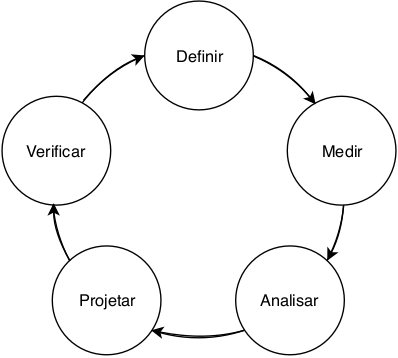
\includegraphics[width=0.5\columnwidth]{images/meth/DMADV.png}
\par\end{centering}

\label{fig:DMADV}
\end{figure}

A figura \ref{fig:DMADV} ilustra o ciclo de trabalho através desta metodologia. Por permitir uma maior flexibilidade na geração das especificações do projeto e
por não requerer uma extrema adaptação do método para produtos de \textit{hardware} e \textit{firmware}, este ciclo será o adotado ao longo do desenvolvimento 
deste projeto. 

Uma visão macro do ciclo empregado ao longo do desenvolvimento deste projeto, com base na metodologia escolhida, é detalhada como:

\begin{enumerate}
    \item Definição dos objetivos gerais do robô;
    \item Definição de requisitos técnicos buscados, como \textit{payload}, velocidade de atuação, precisão de posicionamento e capacidade de repetição de tarefas;
    \item Análise e comparação dos diversos tipos de atuadores, sensores, circuitos acionadores, processadores e controladores que podem ser empregados;
    \item Seleção de elementos com base na etapa passada e projeto das conexões entre estes;
    \item Verificação da adequação do sistema final proposto aos objetivos iniciais, otimização com base em diferenças observadas pela realimentação dessas em um novo ciclo de trabalho.
\end{enumerate}

A etapa de análise conta com o estudo de uma diversa gama de elementos para diferentes fins, para facilitar essa análise está será dividida em ciclos menores de 
trabalho paralelos para o projeto de atuadores e sensores, e em seguida, ciclos para o projeto dos circuitos de acionamento, processamento e controle, da seguinte
maneira:

\begin{enumerate}
    \item \begin{enumerate}
        \item Representação dos objetivos gerais em função dos atuadores e sensores;
        \item Levantamento de requisitos de torque, velocidade, precisão, custo e afins para atuadores e requisitos de precisão, disponibilidade, custo e afins para sensores;
        \item Análise em paralelo de sensores e atuadores que cumprem os respectivos requisitos;
        \item Seleção de elementos com base na análise;
        \item Verificação do cumprimento dos requisitos e otimização, início de novo ciclo para correção de parâmetros.
    \end{enumerate}
    \item \begin{enumerate}
        \item Levantamento de objetivos gerais para circuitos de acionamento;
        \item Geração de requisitos elétricos com base nos atuadores selecionados;
        \item Análise de topologias e elementos de potência para acionamento;
        \item Seleção;
        \item Testes e verificação de corretude do projeto de acionamento para os atuadores propostos.
    \end{enumerate}
    \item \begin{enumerate}
        \item Levantamento de objetivos gerais para circuitos de processamento e controle;
        \item Geração de requisitos de elementos condicionadores e processadores com base nos resultados de etapas passadas;
        \item Análise de possíveis soluções;
        \item Seleção;
        \item Verificação da comunicação entre todos os sistemas.        
    \end{enumerate}
\end{enumerate}

Em cada uma das etapas de verificação é possível que seja necessário uma revisão do que foi proposto na etapa anterior, dando continuidade aos ciclos até que todo
o sistema como um todo seja identificado como uma boa solução no macro ciclo de trabalho.

% Eplicar porque essa vai ser a melhor

\section{Motores}
Iniciando a seleção pelas juntas 5 e 6, que demandam um torque mais 
reduzido em comparação a outras juntas e realizam movimentos relativos ao
punho do manipulador, seria interessante empregar atuadores pequenos 
fisicamente mas que consigam fornecer a potência requerida pelo sistema, 
mantendo o efetuador final simples e sem muitas restrições mecânicas. 
No quesito de potência elétrica consumida, é ideal a escolha de atuadores 
eficientes que não resultem em gastos indesejados e evitáveis. Como o 
acionamento de motores de passo demanda sempre a corrente especificada, 
independente da carga, os motores de rotação contínua seriam uma melhor 
opção. Entretanto, para economizar potência na utilização de motores de 
passo, é possível desligar o seu acionamento quando este não estiver em 
uso, evitando perda por efeito Joule nas suas bobinas. 

Motores DC de rotação contínua apresentam também uma relação potência/peso 
frequentemente melhor frente aos motores de passo, garantindo mais um 
ponto positivo na escolha deste tipo de componentes. 
Ambos os tipos de atuadores em questão apresentam métodos de acoplamentos 
simples. Em relação ao acionamento e preço os motores de passo e motores 
com escova são as melhores opções, já em relação à durabilidade, os 
motores DC sem escovas, incluindo os motores de passo, apresentam uma 
vantagem frente aos aos motores DC escovados. Por fim, os motores de passo 
apresentam um bom comportamento mesmo em malha aberta, já outros tipos de 
motores DC requerem um maior processamento e componentes extras de 
sensoriamento e transmissão para obter resultados semelhantes, tanto em 
torque quanto precisão. 

Utilizando os parâmetros dispostos na seção de análise e pesos atribuídos 
a estes parâmetros, é possível simplificar a escolha dos atuadores para 
estas duas juntas em uma matriz de decisão, onde são atribuidas notas de 
1 a 5 para cada atuador, com base no cenário analisado, onde 5 indica uma 
ótima adequação. 
A matriz de decisão está representada na forma da tabela \ref{tab:SelAtuadores56}.

\begin{table}[h]
\begin{centering}    
    
\begin{tabular}{|c|c|c|c|c|}
    \hline
     & & Motor de passo & Motor DC com escovas & Motor DC sem escovas \tabularnewline
    \hline
    Parâmetro & Peso & & & \tabularnewline 
    \hline
    \hline
    Potência consumida & 3 & 2 & 3 & 4 \tabularnewline
    \hline
    Precisão & 3 & 4 & 2 & 2 \tabularnewline
    \hline
    Massa & 2 & 1 & 3 & 4 \tabularnewline
    \hline
    Inserção & 1 & 4 & 4 & 4 \tabularnewline
    \hline    
    Acionamento & 2 & 3 & 4 & 1 \tabularnewline
    \hline
    Custo & 4 & 3 & 3 & 1 \tabularnewline
    \hline
    Durabilidade & 4 & 3 & 2 & 4 \tabularnewline
    \hline    
    \hline
    Resultado & - & 54 & 53 & 52 \tabularnewline
    \hline
\end{tabular}

\caption{Matriz de decisão para os atuadores das juntas 5 e 6.}
\label{tab:SelAtuadores56}

\par\end{centering}
\end{table}

Nota-se pela tabela \ref{tab:SelAtuadores56} que os parâmetros de torque, 
velocidade e potência mecânica não foram considerados, isto se deve ao 
fato destes fatores serem limitantes, logo, algum tipo de motor que não 
satisfaça essas condições não deve ser considerado para a seleção. 
Os maiores pesos foram escolhidos para o custo e durabilidade do atuador 
empregado, pois estes dois fatores que garantem de fato um resultado de 
baixo custo final, e portanto, um projeto realizável. A potência consumida 
recebeu peso 3 pois este parâmetro infere no tempo de funcionamento do 
braço robótico em sua aplicação real, alimentado por uma bateria, portanto, 
uma maior eficiência é buscada por parte dos atuadores. A importância dada 
à precisão se refere ao fato de facilitar a utilização por parte do usuário 
final. A massa e o acionamento foram levados em consideração pois estes 
fatores afetam diretamente a escolha de outros componentes do sistema, 
como \textit{drivers} e até outros acionadores. Por fim, a inserção não 
afetou a escolha dos atuadores, pois está é realizável de maneira semelhante 
para qualquer tipo de atuador escolhido. Em relação ao atuador da base, a 
matriz de decisão empregada para as juntas 5 e 6 pode ser mantida, 
novamente indicando a seleção por motores de passo. Desse modo, manteve-se 
a escolha original pelos atuadores do tipo 42HS48-1684/NEMA 17 nas juntas 
5 e 6 e modelo HT23-397/NEMA 23 para a base, sendo esta escolha resumida 
na tabela \ref{tab:SelecaoPasso}.

\begin{table}[h]
\begin{centering}  

\begin{tabular}{|c|c|c|c|}
    \hline
    Junta & Atuador selecionado & Ângulo de passo (º) & \textit{Holding} Torque (N.m)\tabularnewline
    \hline
    \hline
    1 & HT23-397/NEMA 23 & 1.8 & 1.25 \tabularnewline
    \hline
    5 e 6 & 42HS48-1684/NEMA 17 & 1.8 & 0.39 \tabularnewline
    \hline
\end{tabular}

\caption{Especificações dos motores de passo selecionados.}
\label{tab:SelecaoPasso}

\par\end{centering}
\end{table}  

Para os motores responsáveis pela movimentação dos elos 1, 2 e 3, a 
principal mudança dos pesos na decisão concentra-se na massa adicionada 
ao sistema. Observando-se que o torque necessário para movimentar estas 
juntas é elevado, o fator potência/peso se torna mais relevante 
à escolha, favorecendo a escolha por motores DC de rotação contínua 
escovados e não motores de passo. 
Os motores originalmente propostos são do tipo Mabuchi JC/LC-578VA, 
que utilizam internamente uma transmissão de torque por um 
par de engrenagens do tipo rosca sem fim, não sendo necessário o consumo 
de potência pelo motor para se manter em uma posição específica. Estes 
motores fornecem, de acordo com a sua ficha catalográfica, 9.12N.m, o que 
não seria suficiente para satisfazer a condição de movimentação para a 
junta 3, que necessita de 9.5N.m, desse modo, faz-se necessário que seja 
selecionado outro motor ou modificada a relação de engrenagens escolhida 
para esta junta. Optou-se pela segunda opção, visto que este motor 
propicia alguns benefícios, como torque de saída elevado e modelo de 
transmissão interna que reduz o consumo de potência.

A tabela \ref{tab:SelecaoDC} contém algumas informações acerca deste manipulador.

\begin{table}[h]
\begin{centering}  

\begin{tabular}{|c|c|c|c|}
    \hline
    Junta & Atuador selecionado & Máximo Torque (N.m) & Velocidade máxima (rad/s)\tabularnewline
    \hline
    \hline
    2, 3 e 4 & Mabuchi JC/LC-578VA & 9.12 & 9.42 \tabularnewline
    \hline
\end{tabular}

\caption{Especificações do motor DC selecionado.}
\label{tab:SelecaoDC}

\par\end{centering}
\end{table}  

\begin{comment}
Introdução
\end{comment}
\chapter{Introdução}

\label{CapIntro}

% Resumo opcional. Comentar se não usar.
%\resumodocapitulo{Resumo opcional}

\section{Contextualização}

A Constituição Federal Brasileira, em seu artigo 5º, define:

\begin{quoting}[rightmargin=0cm,leftmargin=4cm]
%\begin{singlespace}
{\footnotesize 
``Art. 5º. Todos são iguais perante a lei, sem distinção de qualquer natureza, garantindo-se aos brasileiros e aos estrangeiros residentes no 
País a inviolabilidade do direito à vida, à liberdade, à igualdade, à segurança e à propriedade[...]''
\\ (Constituição Federal, 1988)\cite{constituicao}.
}
%\end{singlespace}
\end{quoting}

Baseando-se na igualdade proposta e elevando este conceito acima do nível simplesmente nacional, são propostas frequentemente novas tecnologias que buscam proporcionar 
ou ampliar habilidades funcionais de pessoas com deficiência, garantindo autonomia e igualdade em questão de acessibilidade a estas pessoas, promovendo por 
fim a sua independência e inclusão. Para se referir a este tipo de tecnologias, é comumente utilizado o termo Tecnologia Assistiva - TA \cite{bersch2008introduccao}.  

Sancionado em 2015, o Estatudo da Pessoa com Deficiência fornece uma definição para acessibilidade no âmbito nacional:

\begin{quoting}[rightmargin=0cm,leftmargin=4cm]
%\begin{singlespace}
{\footnotesize 
``I - acessibilidade: possibilidade e condição de alcance para utilização, com segurança e autonomia, de espaços, mobiliários, equipamentos urbanos, 
edificações, transportes, informação e comunicação, inclusive seus sistemas e tecnologias, bem como de outros serviços e instalações abertos ao público,
de uso público ou privados de uso coletivo, tanto na zona urbana como na rural, por pessoa com deficiência ou com mobilidade reduzida;''\\
(Estatuto Da Pessoa com Deficiência, 2015)\cite{estatutodef}.
}
%\end{singlespace}
\end{quoting}

Assim, pessoas com deficiência motora, que têm em sua condição uma autonomia reduzida, possuem também uma menor acessibilidade geral, sendo necessário fornecer
meios de ampliar sua independência, respeitando os seus direitos fundamentais. A autonomia em questão é afetada diretamente pelo tipo de lesão ou 
má-formação observada: a paraplegia, ou ausência de membros inferiores, dificulta a a locomoção, já a tetraplegia chega a restringir quase toda a movimentação do deficiente.
Na pesquisa por novas Tecnologias Assistivas para incrementar a autonomia nestes casos, há o ramo de desenvolvimento de braços mecânicos assistivos, podendo 
estes serem fixos em determinado local, ou móveis, como quando são acoplados em cadeiras de rodas. Enquadrando-se na categoria de TA de auxílio para vida
diária e vida prática, os braços robóticos montados sobre cadeiras de rodas (\textit{WMRA - Wheelchair Mounted Robotic Arm}), assim como outras tecnologias 
assistivas, têm como finalidade permitir um bom desempenho em atividades diárias básicas (\textit{ADL} - Activities of Daily Living) \cite{capille2010kinematic}. 

Tendo em vista que, em 2010, 15\% da população mundial vivia com algum tipo de deficiência \cite{world2011world}, os avanços buscados em tecnologias 
assistivas são de grande importância, pois afetam grande parte da população, direta e indiretamente, 
garantindo maior liberdade a pessoas com deficiência e uma sociedade
mais igualitária, alinhando-se com a agenda 2030 da ONU - Organização das Nações Unidas,
para desenvolvimento sustentável, especificamente com a meta 10 - Redução das Desigualdades \cite{un2030agenda}.

\section{Definição do problema}

Foi idealizada e construída na Universidade de Brasília - UnB, no período de 2018 a 2019, 
a estrutura mecânica de um braço robótico a ser montado em uma cadeira de rodas, com a finalidade de ser
uma solução barata e suficiente para aprimorar a acessibilidade de pessoas que sofreram lesão medular completa do tipo tetraplegia \cite{fernando2019assistivo}. 
O projeto base conta com uma seleção inicial de atuadores para as juntas deste, no entanto, para garantir uma adequação real do braço construído como 
tecnologia assistiva, faz-se necessário que o braço possa ser controlado pelo usuário final, sendo essencial para isto a verificação dos atuadores selecionados, 
inserção de elementos sensoriais no manipulador, projeto de uma plataforma de controle e junção eletro-eletrônica desta com os atuadores e sensores propostos.

\subsection{Estrutura do manipulador robótico base}
\label{sec:EstruturaBase}

O braço robótico em questão é do tipo articulado, possui 3 juntas principais e um punho implementado como 3 juntas rotativas com eixos que não se cruzam em um
mesmo ponto. A primeira junta constitui a rotação do robô em torno de sua base, a segunda é denominada como ombro, a terceira como cotovelo e as juntas do 
punho são divididas com base no tipo de movimento de rotação que causam, sendo estes denominados como rolagem, arfagem e guinada. As juntas do robô são 
construídas majoritariamente de chapas de alumínio conformado, os elos por sua vez foram projetados com material PVC e \textit{Nylon (TechNyl)}. 

Foram selecionados para o acionamento do manipulador 3 motores do tipo Mabuchi JC/LC-578VA, 1 motor de passo HT23-397/NEMA 23 e 2 motores de passo 
42HS48-1684/NEMA 17. Para a transmissão do torque de saída dos atuadores propostos até o ponto de atuação foi idealizada uma transmissão por engrenagens,
sendo as engrenagens fabricadas com tecnologia de manufatura aditiva e materiais PLA e ABS. Para o controle do robô foi proposto inicialmente um Arduino, 
no entanto, esta escolha deve ser revista após a revisão dos atuadores e seleção de sensores e circuitos de ativação e processamento. 

A modelagem gráfica do manipulador pode ser vista na figura \ref{fig:manipulador-base}.

\begin{figure}[h]
\caption{Modelagem do robô montado \cite{fernando2019assistivo}.}    
\begin{centering}
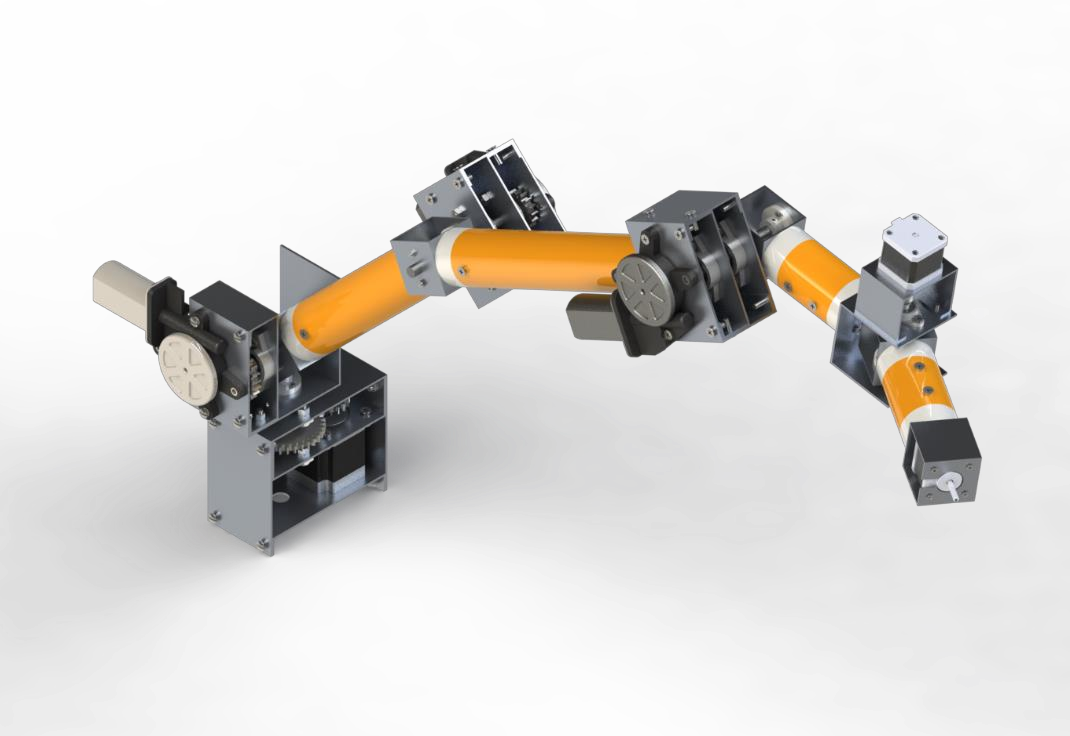
\includegraphics[width=0.9\columnwidth]{images/intro/manipulador-base.png}
\par\end{centering}

\label{fig:manipulador-base}
\end{figure}

Nota-se pela figura o local de aplicação dos atuadores selecionados, assim como descrito na tabela \ref{tab:AtuadoresPre}. A figura demonstra também como
foram empregados os tubos de material PVC e acopladores de \textit{Nylon} na construção dos elos, bem como o formato das juntas com uma separação para inserção
das engrenagens que compõem a relaçãos calculadas no projeto base \cite{fernando2019assistivo}.

\begin{table}[h]
\begin{centering}  

\begin{tabular}{|c|c|}
    \hline
    Junta & Atuador selecionado \tabularnewline
    \hline
    \hline
    1 (Base) & HT23-397/NEMA 23 \tabularnewline
    \hline
    2 (Ombro) & Mabuchi JC/LC-578VA \tabularnewline
    \hline
    3 (Cotovelo) & Mabuchi JC/LC-578VA \tabularnewline
    \hline
    4 (Arfagem) & Mabuchi JC/LC-578VA \tabularnewline
    \hline
    5 (Guinada) & 42HS48-1684/NEMA 17 \tabularnewline
    \hline
    6 (Rolagem) & 42HS48-1684/NEMA 17 \tabularnewline
    \hline
\end{tabular}

\caption{Atuadores pré-selecionados para as juntas.}
\label{tab:AtuadoresPre}

\par\end{centering}
\end{table}

\section{Objetivos do projeto}

O objetivo principal deste trabalho é analisar o braço robótico apresentado na seção \ref{sec:EstruturaBase} a fim de revisar os atuadores existentes neste e
propor instrumentos de medição e circuitos de acionamento e processamento para serem inseridos em sua estrutura, bem como idealizar um controlador para reger 
os movimentos deste manipulador robótico. 
Os circuitos eletro-eletrônicos e o sistema de controle propostos devem
ser capazes de receber comandos do usuário e acionar os atuadores de 
maneira a permitir que a estrutura mecânica subjacente e o efetuador 
final do manipulador sejam posicionados de acordo a auxiliar o operador 
na interação com o espaço ao seu redor para a realização de atividades
diárias básicas.

Pautando-se em um dos objetivos do trabalho base, o manipulador, com 
todo o sistema de sensoriamento, ativação e controle, deve apresentar 
um baixo custo, para que possa ser considerado um protótipo acessível
para auxílio de pessoas com deficiência motora dos membros inferiores 
e superiores.

% Escrever sobre metodologia? 
%\section{Metodologia de desenvolvimento}

\section{Apresentação do trabalho}

O trabalho foi organizado em 6 capítulos. O primeiro capítulo é 
introdutório, indicando as motivações e objetivos do projeto. 
No Capítulo 2 é apresentada uma revisão bibliográfica sobre projetos
semelhantes, da mesma forma são expostos modelos comerciais de WMRAs, 
servindo como possíveis fontes de inspiração e comparação com o produto 
a ser desenvolvido neste trabalho. No mesmo capítulo são também revisados
conceitos teóricos que forneceram o embasamento técnico para a 
realização do projeto. 

O desenvolvimento foi dividido em 2 capítulos, Capítulo 3, onde
são enunciados os objetivos, diretrizes e escolhas realizadas quanto 
ao desenvolvimento dos diversos circuitos eletro-eletrônicos, e 
Capítulo 4, que descreve a maneira como o controlador geral do robô foi
implementado.

O Capítulo 5 contém resultados observados ao longo do desenvolvimento,
tanto obtidos por simulações como através de protótipos construídos, 
para comparação entre os objetivos propostos e resultados de fato obtidos.
No Capítulo 6 encontram-se as considerações finais do projeto, com 
uma conclusão pautada em tudo o que foi observado durante a realização
do projeto e perspectivas futuras para possíveis trabalhos que possam 
emanar do projeto desenvolvido. 

\begin{comment}
Fundamentos
\end{comment}

\chapter{Fundamentação Teórica\label{chap:FundamentacaoMatematica}}

% Revisar a citação de motores elétricos CHAPMAN

% Resumo opcional. Comentar se não usar.
%\resumodocapitulo{Resumo opcional.}

\section{Revisão Bibliográfica}
\label{sec:revisaobib}

A idealização, construção e controle de braços robóticos montados sobre cadeiras de rodas é um foco de pesquisa amplo, 
sendo desenvolvidos projetos tanto na área comercial quanto na área de 
pesquisa universitária, resultando em diferentes produtos com focos distintos. 
É interessante estudar os tipos de tecnologias, características e funcionalidades
propostas nos diversos trabalhos desenvolvidos, tanto para tecnologias 
assistivas quanto para tecnologias semelhantes, para se ter uma boa base
no desenvolvimento de um novo projeto, que busque apresentar algum 
diferencial frente às tecnologias já existentes.

Na Universidade de Brasília, já foram desenvolvidos projetos envolvendo a adaptação, controle e instrumentação de cadeiras de rodas para deficientes. 
Uma vez que os braços robóticos são montados sobre estas, é importante analisar estes projetos a fim de estudar tecnologias de alimentação e acoplação para o braço 
proposto. Foi apresentado, em conjunto com a Universidade Federal de Pernambuco e outras partes, um \textit{kit} de automação para cadeiras de rodas convencionais 
\cite{vidal2010desenvolvimento}, sendo este de extrema importância por já demonstrar as dimensões e limitações básicas de uma cadeira de rodas convencional, 
o tipo e posicionamento do circuito de alimentação e componentes eletro-eletrônicos comumente empregados neste tipo de projeto.
O trabalho apresentado em \cite{francisco2019interface} foca no desenvolvimento de uma interface para que o operador possa controlar a cadeira de rodas
de forma satisfatória, fornecendo ideias para uma interface viável também para o controle do braço robótico a ser acoplado neste tipo de cadeira de rodas.

Os projetos citados demonstram que é comum a utilização de baterias 
automotivas como fonte de energia ao sistema de locomação, podendo esta mesma bateria
servir também como alimentação para um braço robótico acoplado à cadeira 
de rodas, fornecendo uma tensão nominal comum de 12V.
Também é notável a escolha por motores de corrente contínua, ou simplesmente
motores DC, para este tipo de tecnologia, com acionamento controlado através de 
circuitos do tipo ``Ponte H''.

Embora não tenham sido encontrados especificamente projetos acerca de WMRA na Universidade de Brasília, foram identificados projetos de braços robóticos
construídos para outros fins, sendo uma análise desses imprescindível para se ter conhecimento acerca do tipo de atuadores e sensores comumente empregados em 
braços robóticos no geral.

%\subsection{Manipulador robótico didático}
Um manipulador didático, desenvolvido em \cite{wattylas2015didatico} e aprimorado em \cite{marconi2016didatico}, apresenta uma estrutura semelhante a do trabalho base
deste projeto, em relação ao posicionamento relativo das juntas iniciais, como pode ser visto na figura \ref{fig:manipulador-didatico}.

\begin{figure}[ht]
\caption{Modelagem do robô didático \cite{wattylas2015didatico}.}    
\begin{centering}
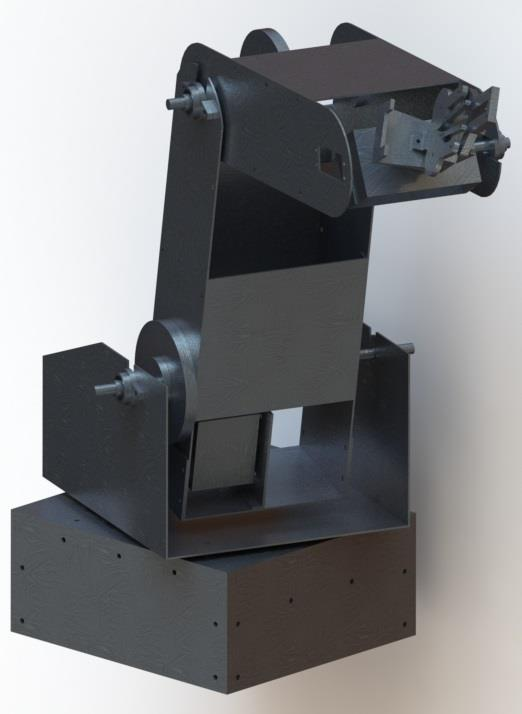
\includegraphics[width=0.5\columnwidth]{images/fundamentos/manipulador-didatico.png}
\par\end{centering}

\label{fig:manipulador-didatico}
\end{figure}

O projeto em questão tem como foco a interação entre o braço e pessoas com a finalidade de estimular e auxiliar o aprendizado no ramo da engenharia.
Embora este manipulador não seja do tipo WMRA, os circuitos de 
acionamento projetados e o método de controle desenvolvido podem ser 
levados em consideração no projeto atual, demonstrando a importância da
análise deste sistema.
A estrutura do robô apresenta uma base e três juntas com eixos paralelos
em sequência, em convergência com o modelo base para este projeto, desse modo,
pontos de desenvolvimento acerca da cinemática inversa podem ser comparados
e reutilizados.

Neste trabalho são expostas também a escolha por motores de passo em 
algumas juntas e uma ideia de \textit{driver} para controle destes, 
levantando a possibilidade de uso desse tipo de motores em projetos 
de manipuladores robóticos.

%\subsection{WMRA - USF}
Foi desenvolvido na \textit{Universisty of South Florida} um robô com motivações semelhantes à deste projeto \cite{kevin2005WMRA}, buscando atender às 
necessidade de pessoas com mobilidade reduzida e redução de custos deste tipo de tecnologia. O manipulador final apresenta 7 graus de liberdade, onde todas as
juntas são acionadas por motores DC escovados servo-controlados e controladas em conjunto através de placas 
controladoras baseadas na arquitetura PIC.
Uma foto do braço construído pode ser vista na figura \ref{fig:wmra-usf}.

\begin{figure}[ht]
\caption{Braço robótico completo construído na USF \cite{kevin2005WMRA}.}    
\begin{centering}
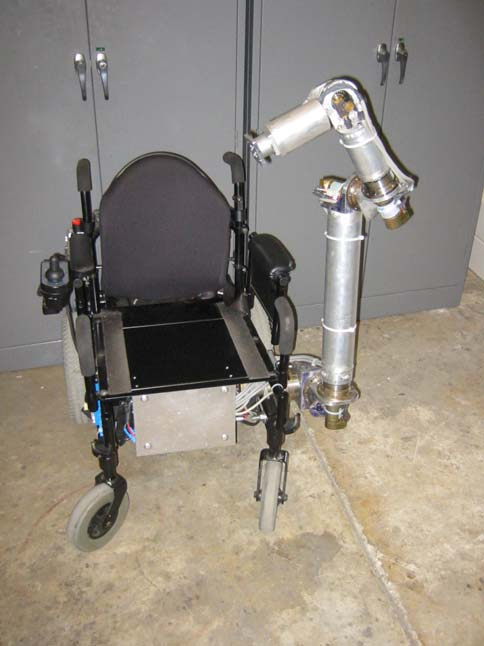
\includegraphics[width=0.5\columnwidth]{images/fundamentos/wmra-usf.png}
\par\end{centering}

\label{fig:wmra-usf}
\end{figure}

O manipulador final, com uma massa de 12.5kg, tem a capacidade de atingir uma altura máxima de 1.37m acima do chão e suporta uma carga, ou \textit{payload}, de até
6kg. Há dois pontos principais que devem ser observados no resultado final obtido pelo 
projeto citado, no que diz respeito a este projeto. 
O primeiro ponto de interesse está na utilização de caixas de engrenagens
harmônicas, que permitem uma alta relação de transmissão de torque, facilitando
a escolha dos motores utilizados.
O segundo ponto está nas unidades de controle aplicadas, apresentando 
características importantes no controle de motores DC, como controle PID
de posição e velocidade, comunicação RS-485 e leitura integrada de diversos
sensores, fatores que também devem ser levados em consideração no desenvolvimento
deste projeto.

Além dos modelos de braço robótico resultantes de estudos em universidades, 
há diversos tipos de modelos de WMRA existentes no mercado, apresentando 
geometrias, método de atuação, alcances e \textit{payloads} diferentes. 
O estudo desses modelos fornece uma boa base para novos projetos, podendo 
o modelo proposto ser comparado aos modelos comerciais a fim de se analisar 
a adequação da solução proposta ao mundo real.

Entre os modelos comerciais encontram-se o sistema JACO, construído pela empresa Kinova, o sistema MANUS e sua evolução iARM, desenvolvidos pela \textit{Assistive
Innovations} e o modelo \textit{Raptor}, fabricado pela \textit{Applied Resources} \cite{ktistakis2015survey}, onde cada um desses modelos pode ser levado em 
consideração na geração de especificações para um novo braço robótico com finalidade semelhante.
Em relação aos modelos comerciais, os fatores de comparação que mais
impactam este projeto seriam a velocidade linear atingível, tensão de 
alimentação, consumo e interface homem-máquina, outros fatores como alcance, peso e \textit{payload}
foram importantes no momento de decisão da estrutura mecânica no manipulador. 

Um estudo destes modelos demonstra que \textit{joysticks} são frequentemente 
utilizados como uma possibilidade de interface entre o operador e o robô \cite{capille2010kinematic},
sendo este modelo de interface adotado também na execução deste trabalho.

\section{Atuadores}
Em relação aos atuadores utilizados em manipuladores robóticos, há a possibilidade de emprego de atuadores do tipo hidráulico, pneumático e/ou eletromagnéticos, 
dentre outros, onde cada tipo de atuador apresenta pontos fortes e fracos para a aplicação em questão. 

Os atuadores hidráulicos são empregados geralmente por sua capacidade de gerar forças e torques elevados, com um controle simples, no entanto, embora os 
atuadores em si normalmente sejam compactos, é necessário uma grande quantidade de equipamentos extras para garantir o funcionamento e segurança destes, como
bomba, mangueiras, válvulas e acumuladores. Por sua vez, os atuadores pneumáticos apresentam uma capacidade de gerar forças um pouco inferiores àquelas atingidas 
por atuadores hidráulicos mas em velocidades mais elevadas, e também não necessitam de meios de contenção de líquidos, outrora utilizados em meios hidráulicos, 
porém, apresentam em geral um controle menos preciso com precisão afetada pela compressibilidade do ar e atrito interno dos atuadores \cite{hunter1991comparative}. 
Nestas duas classes de atuadores os mais utilizados são os atuadores lineares, porém há também os atuadores rotativos e atuadores do tipo músculo.

No que diz respeito aos atuadores elétricos, estes vem ganhando uma grande participação na aplicação em manipuladores, principalmente pela quantidade de 
alternativas de faixas de torque e velocidade, além de poderem apresentar um controle mais simples e fino. Entre os motores elétricos há aqueles operados
por corrente alternada e aqueles acionados por uma corrente contínua, sendo que a principal diferença entre estes encontra-se no método de controle
da velocidade de rotação. Os motores de corrente alternada, ou motores AC, são geralmente mais robustos e tem a sua velocidade controlada através da frequência
de oscilação da alimentação, sendo utilizados majoritariamente em aplicações com potência elevada e uma velocidade contínua com pequenas variações. Dentro da categoria de motores de corrente contínua existe uma diversa gama de modelos de atuadores, 
como motores DC de imã permanente, de excitação independente e em série, sendo diferenciados também pela presença de escovas ou não \cite{chapman2005electric}. 
Os motores DC podem apresentar um tamanho mais reduzido para aplicações mais simples, além de necessitarem de circuitos acionadores frequentemente mais simples em 
relação aos motores AC.

\section{Sensoriamento e Condicionamento}
Para se garantir eficiência e precisão durante a operação de um robô, é essencial a utilização de sensores, sendo neste ramo de pesquisa os sensores
divididos em sensoriamento interno, como no caso de medição da posicão, velocidade e torque das juntas, ou sensoriamento externo, como sensores próprios para 
visão, e medição de força e distância \cite{bajd2010robotics}.

Em um sistema de medição, geralmente são identificados quatro tipos de elementos, sendo os elementos do tipo sensor o primeiro desses. Usualmente são empregados
em conjunto com sensores elementos de condicionamento, processamento e de apresentação de dados, para garantir que a leitura desejada será devidademente medida
e tratada \cite{bentley2005principles}.

Na categoria de sensores que podem ser utilizados para se monitorar posicionamento as principais escolhas seriam os potênciometros, \textit{encoders} ópticos, 
sensores indutivos e de efeito \textit{hall}. Entre estes sensores de posicionamento, há aqueles que fornecem informações relativas à uma posição inicial e aqueles
capazes de fornecer uma informação acerca de um posicionamento absoluto mensurado \cite{bentley2005principles}. Sensores de toque, ou fim-de-curso, podem ser utilizados
a fim de se ter conhecimento do estado das juntas de um robô em determinada posição, auxiliando em um posicionamento correto no espaço.

Para se ter uma ideia do torque interno das juntas de um robô podem ser empregados também sensores do tipo \textit{hall}, no caso de juntas com motores elétricos, 
com o objetivo de se mensurar e auxiliar no controle da corrente que chega nos atuadores, diretamente relacionada com o torque resultante. A fim de mensurar ações de forças 
externas são comumente empregadas células de carga, que constituem um sistema de medição com extensômetros e condicionadores de sinal. O uso de extensômetros nos 
elos de um manipulador permite obter informações sobre ações externas e deformação que agem sobre estes, podendo estas serem usadas de modo a garantir uma maior
segurança durante a operação do manipulador.

Alguns fatores importantes na escolha de elementos sensores são a 
resolução, histerese, limiar de medição e zona morta dos mesmos, 
fatores estes que influenciam a acurácia e precisão da leitura. 
Instrumentos de medição do tipo \textit{encoder} e potenciômetros 
estão sujeitos a uma certa resolução, que é definida em \cite{doebelin2007measurement} 
como a menor quantidade possível de variação na entrada que resulta 
em uma mudança do valor de saída, sendo imprescindível escolher um 
dispositivo que forneça uma resolução boa o suficiente para que o 
posicionamento dos elos e juntas de um manipulador seja conhecido 
com baixa incerteza.

Demais instrumentos de tratamento de sinal também estão sujeitos a estas
condições de operação, conversores analógicos-digitais - ADC, por exemplo, possuem
uma resolução relacionada com a quantidade de \textit{bits} utilizados
na conversão de valores, sendo importante atentar-se a este tipo de 
elemento em um circuito de instrumentação \cite{bentley2005principles}. 
Esta relação de resolução pode ser vista na equação \ref{eq:res_adc}, 
onde a resolução foi indicada
por $\rho$ e $n$ indica a quantidade de bits disponíveis no conversor.

\begin{equation}
    \label{eq:res_adc}
    \rho = \frac{1}{2^n}
\end{equation}

Tratando-se de resolução, \textit{encoders} rotativos apresentam características
semelhantes aos conversores citados, por possuirem uma quantidade de posições  
que se equipara à quantidade de bits em um ADC. 
A resolução destes pode ser definida de acordo com
a equação \ref{eq:res_encoder}, onde $PPR$ identifica a quantidade de 
pulsos, ou posições, por revolução. Esta resolução pode ser aprimorada
incluindo-se uma relação de transmissão entre o eixo da junta e o sensor,
aumentando assim a escala de saída do sensor para uma mesma escala
de entrada, fazendo com que o mesmo valor na entrada possua uma gama maior
de relação com a saída, superando a resolução básica do sensor.

\begin{equation}
    \label{eq:res_encoder}
    \rho = \frac{2\pi}{PPR}
\end{equation}

Potenciômetros podem também estar sujeitos às limitações impostas 
pela resolução, como no caso de potenciômetros construídos com fios 
enrolados, no entanto, outros modelos, como os de plástico condutivo,
não estão sujeitos a estes efeitos \cite{bentley2005principles}.

Em relação à transmissão de sinais elétricos, o devido cuidado deve
ser tomado para evitar que ruídos e interferências afetem o sinal de 
modo a inserir erro no funcionamento geral do sistema. 
As fontes de ruído são divididas em internas e externas. Uma possível fonte de
ruído interna é a movimentação de cargas em elementos condutores 
devido à temperatura, por esse motivo este tipo de ruído é denominado 
ruído térmico, ou ruído de Johnson-Nyquist, sendo considerado uma forma de
ruído branco, por apresentar uma densidade espectral aproximadamente 
constante. Circuitos AC ou circuitos com chaveamento próximo ao sistema 
são, por sua vez, fontes comuns de ruído externo, 
podendo gerar transientes no sinal transmitido \cite{bentley2005principles}.

Os ruídos e demais interferências sobre um sistema elétrico podem ser 
considerados como em série, apresentando-se como uma fonte de 
diferencial de potencial entre o sistema emissor e receptor do sinal, 
ou de modo comum, onde os potenciais de ambos emissor e receptor estão
sujeitos a uma variação de potencial referente ao ruído que age sobre o sistema \cite{bentley2005principles}.

\begin{figure}[h]
    \caption{Interferência causada por múltiplos terras.}    
    
    \begin{centering}
        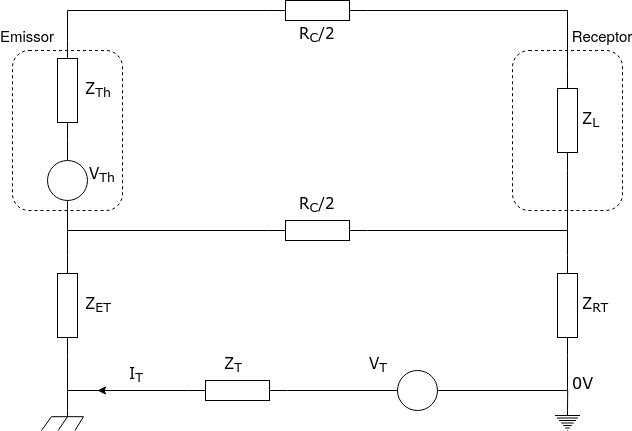
\includegraphics[width=0.7\columnwidth]{images/fundamentos/Interferencia.png}
    \par\end{centering}

    \label{fig:interferencia}
\end{figure}

A figura \ref{fig:interferencia} ilustra interferência causada pelo
problema comum de múltiplos terras, onde pontos que teoricamente deveriam
apresentar o mesmo potencial de 0V possuem entre si uma diferença de 
potencial, representada por $E_T$, causada por descarga de equipamentos ou quaisquer 
outros fatores. Esta diferença de potencial faz com que apareça no sistema 
uma corrente $I_T$, gerando tanto uma interferência de modo comum, ao 
induzir uma tensão sobre a impedância entre o receptor e o plano de terra
real, $Z_{RT}$ e um interferência em série, através da diferença de 
tensão que surge sobre a resistência do cabo $R_C/2$. Por esse motivo, é 
essencial que o sistema de medição seja conectado ao plano de terra em 
um único ponto, quando não é possível garantir o mesmo potencial no 
emissor e receptor \cite{bentley2005principles}.

Outro fator que pode afetar a integridade de sinais são as reflexões 
e distorções causadas por discontinuidades de impedância ao longo do 
caminho de transmissão. 
Quando um sinal elétrico encontra uma discordância entre pontos de 
diferentes impedâncias, parte dele será refletico de volta à origem,
causando ruídos de reflexão, resultando em uma degradação do sinal. 
A estratégia mais comum para evitar este tipo de reflexão consiste
na inserção de uma resistência próxima ao emissor do sinal, com o valor
necessário para que a soma das impedância dessa nova resistência com a
impedância interna do emissor sejam equivalentes à impedância da linha
de transmissão \cite{bogatin2010signal}. 

Dentre os métodos utilizados para redução dos efeitos de ruídos e 
interferências na transmissão de sinais, são notáveis a importância da
separação do circuito de medição de possíveis fontes de interferência,
como circuitos de potência, uso de técnicas de blindagem em cabos, como
transmissão por par de cabos trançados e/ou uso de camadas específicas de
blindagem, envio e recebimento de sinais diferenciais, isolamento entre
emissor e receptor e tratamento por meio de filtros \cite{bentley2005principles}.

Dentre os filtros implementados no tratamento de sinais encontra-se os
filtros passa-baixo, passa-alto, passa-banda e rejeita-banda \cite{irwin2010basic}. 
Os filtros passa-baixo são utilizados na atenuação de componentes de alta
frequência dos sinais, priorizando as variações de baixa frequência.
Este tipo de filtro é utilizado largamente quando há a necessidade de
filtrar sinais resultantes da mudança de estados de botões, removendo
em grande parte os efeitos de seus transientes mecânicos \cite{ganssle2004guide}.

\begin{figure}[h]
    \caption{Filtro RC.}    
    
    \begin{centering}
        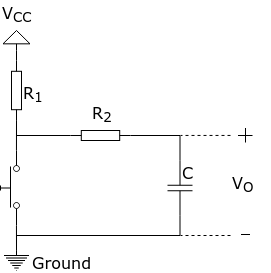
\includegraphics[width=0.3\columnwidth]{images/fundamentos/RCFilter.png}
    \par\end{centering}

    \label{fig:filtrorc}
\end{figure}

Normalmente assumindo o formato representado na figura \ref{fig:filtrorc},
um filtro RC garante uma variação mais bem definida para a saída do 
circuito através do descarregamento e carregamento do capacitor. 
A relação entre o valor de saída e valor de entrada depende do regime
onde se encontra o capacitor, carregamento ou descarregamento. 
As equações que regem esses regimes estão descritas nas fórmulas 
\ref{eq:filtrorc1}, para o carregamento, e \ref{eq:filtrorc2}, para o descarregamento.

\begin{equation}
    \label{eq:filtrorc1}
    V_O = V(t) = V_{CC}\left(1-e^{\frac{-t}{\tau}}\right)
\end{equation}

\begin{equation}
    \label{eq:filtrorc2}
    V_O = V(t) = V(t_0)\left(e^{\frac{-t}{\tau}}\right)
\end{equation}

Em ambos casos a constante de tempo $\tau$ é dada pela multiplicação 
entre a resistência equivalente do circuito e a capacitância, $\tau = RC$.
Nota-se que para o carregamento do capacitor a resistência total do
circuito equivale à soma das resistências de $R_1$ e $R_2$, já no 
descarregamento, somente $R_2$ influencia a constante de tempo. 

Amplificadores operacionais podem também ser usados no condicionamento
de sinais elétricos, sua impedância de entrada idealmente infinita 
evita pertubar o sinal nos terminais de entrada, por demandar pouca 
corrente.
A definição de um ganho em circuito pode também facilitar a leitura 
de sinais pequenos de tensão por equipamentos com baixa precisão, 
elevando um sinal na escala de millivolts para volts.

Quando da aplicação de um circuito integrado (CI) do tipo amplificador
operacional, alguns cuidados devem ser tomados em relação aos
comportamentos não ideais deste, ou imperfeições, 
como tensão e corrente de \textit{offset} \cite{sedra1998microelectronic}.
A rejeição de modo comum, ou CMRR, do inglês \textit{Common-Mode Rejection Ratio},
é uma característica que deve ser observada na aplicação deste tipo de 
CI, onde geralmente é desejado que seja amplificado unicamente a 
diferença de tensão entre os terminais de entrada, e o fator comum
seja desprezível.

Amplificadores operacionais podem ser utilizados no modo inversor ou 
não-inversor, onde cada modelo apresenta seus benefícios e desvantagens.
O modo não-inversor por exemplo apresenta uma resistência de entrada mais
próxima do ideal, mas não permite ganhos inferiores a 1 \cite{sedra1998microelectronic}.
Um arranjo de amplificadores operacionais e resistores de precisão 
pode ser realizado para se obter um outro tipo de amplificador denominado
amplificador de instrumentação, que conta com alta rejeição de modo comum, 
pequenos fatores de não-linearidade, alta impedância de entrada e ganho
diferencial facilmente ajustável \cite{kitchin2006designer}, sendo 
considerado um circuito superior aos amplificadores comuns.

\begin{figure}[h]
    \caption{Configurações de amplificadores operacionais.}    
    
    \begin{centering}
        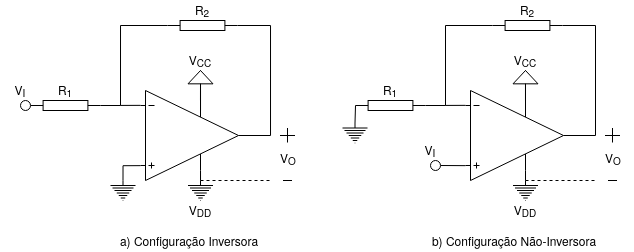
\includegraphics[width=1\columnwidth]{images/fundamentos/AmpOps.png}
    \par\end{centering}

    \label{fig:ampops}
\end{figure}

A figura \ref{fig:ampops} ilustra as configurações mais comuns no uso
de amplificadores operacionais, com uma entrada mantida em um potencial
conhecido. O ganho para a configuração inversora está definido na 
equação \ref{eq:ampop1}, já para a configuração não-inversora, o ganho é 
representado na equação \ref{eq:ampop2}. Para amplificadores de 
instrumentação, o ganho pode ser definido de diversas maneiras, a 
depender do CI empregado.

\begin{equation}
    \label{eq:ampop1}
    V_O = -V_I\left(\frac{R_2}{R_1}\right)
\end{equation}

\begin{equation}
    \label{eq:ampop2}
    V_O = V_I\left(1+\frac{R_2}{R_1}\right)
\end{equation}

As alimentações $V_{CC}$ e $V_{DD}$, observadas na figura \ref{fig:ampops},
são necessárias para o correto funcionamento dos amplificadores em CIs, 
devendo ser respeitados os limites impostos por fabricantes. 
Geralmente a alimentação é simétrica, sendo necessário duas 
fontes de alimentação para que se obtenha o valor correto de saída 
desejado. Todavia, alguns CIs empregam um funcionamento do tipo 
\textit{single-supply}, onde algum dos terminais de alimentação pode 
ser mantido como potencial nulo, ou 0V.
A saída de um circuito do tipo amplificador operacional é limitada 
a uma escala definida por essas duas alimentações, sendo comum esta
escala ser menor que a escala de entrada por alguns volts. 
Amplificadores do tipo \textit{rail-to-rail} permitem que a saída atinja valores mais 
próximos ao valor de alimentação, caso assim seja desejado \cite{mancini2003op}.

Outra maneira de evitar a propagação de interferências da linha ao 
receptor do sinal está no uso de optoacopladores, dispositivos que 
isolam eletricamente o sinal controlador, da carga. A maioria deste 
tipo de equipamento emprega sinais luminosos na faixa de infravermelho 
à luz visível vermelha para o transporte de informação, sem o desgaste
mecânico intrínsico ao funcionamento de relés \cite{temis1996optocouplers}.

\begin{figure}[h]
    \caption{Circuito usual no emprego de optoacoplador.}    
    
    \begin{centering}
        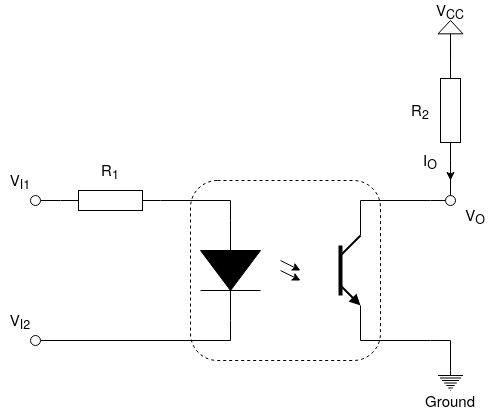
\includegraphics[width=0.6\columnwidth]{images/fundamentos/Optocoupler.png}
    \par\end{centering}

    \label{fig:opto}
\end{figure}

A figura \ref{fig:opto} ilustra o modelo de um optoacoplador, onde o 
sinal de entrada, constituido por $V_{I1}$ e $V_{I2}$ ativa o LED, que
por sua vez causa um sinal luminoso que permita o chaveamento do 
fototransistor \cite{bishop2001understand}. Uma característica importante
sobre o funcionamento de optoacopladores diz respeito à sua taxa de 
transmissão de corrente, isto é, quanto da corrente de entrada o 
dispositivo permite que seja transportado na saída. Denominado como 
CTR, do inglês \textit{Current Transfer Ratio}, esta taxa afeta
diretamente o valor das resistências $R_1$ do circuito, 
pois esta resistência devem ser projetadas de modo que a corrente de 
saída, $I_O$, atinja o valor esperado, e que a corrente de entrada 
esteja sempre no valor de segurança definido pelo fabricante. Caso a 
variável de interesse seja tensão, $V_0$, $R_2$ deve ser inserida no 
circuito com um valor de resistência que resulte em uma diferença de
potencial entre seus terminais de acordo com o desejado.

A corrente de entrada do circuito, ou corrente direta de alimentação 
do diodo, é definida de acordo com a equação \ref{eq:opto1}, em função
da queda de tensão no diodo, $V_f$, sendo possível também expressar a 
resistência $R_1$ em função de uma corrente pré-definida \cite{sedra1998microelectronic}.

\begin{equation}
    \label{eq:opto1}
    I_f = \frac{\left(V_{I1}-V_{I2}\right) - V_f}{R_1}
\end{equation}

Tendo conhecimento da corrente de entrada e do gráfico de CTR para 
determinado positivo, define-se a máxima corrente de saída como
$I_f \cdot CTR$. 

\section{Controle de velocidade}
Uma típica malha de controle pode ser representada em duas formas, denominadas malha aberta ou malha fechada, assim como representado na figura \ref{fig:excontrole},
onde a entrada, ou referência, com interferência ou não da saída, ou variável controlada, alimenta o circuito de controle e este regula o sinal enviado ao processo
para obter assim um valor de acordo com a referência indicada \cite{nise2011control}. 

\begin{figure}[h]
\caption{Formas de representação para controle em malha aberta e malha fechada}    
\begin{centering}
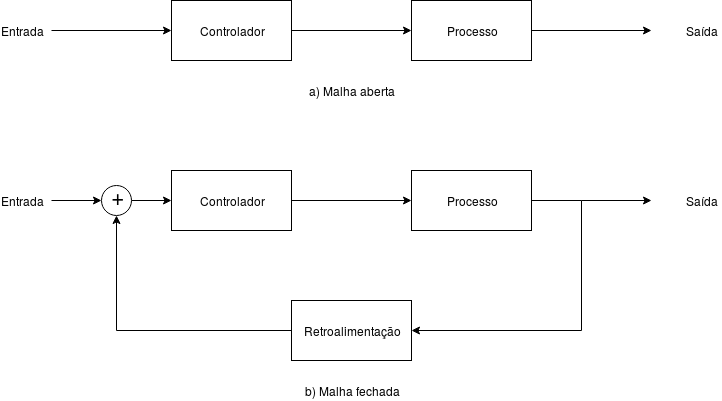
\includegraphics[width=0.8\columnwidth]{images/fundamentos/excontrole.png}
\par\end{centering}

\label{fig:excontrole}
\end{figure}

Em um sistema robótico é comum utilizar alguma malha de controle, como as da figura \ref{fig:excontrole}, para se controlar a posição e/ou velocidade
das juntas do robô, resultando em alguma configuração desejada para este no espaço. 

Para realizar o controle de um manipulador robótico, garantindo
o correto processamento dos dados dos diversos sensores utilizados e o 
acionamento correto dos atuadores, deve ser utilizado um circuito próprio para este fim, como através de um microcontrolador, que 
agrupa em uma mesma placa um processador, memória e portas de entrada e saída de dados, sendo amplamente utilizados em sistemas de medição \cite{bentley2005principles}.
No emprego de um microcontrolador uma importante característica a ser analisada é o seu processador, onde a arquitetura deste afetará
diretamente a implementação do controlador que irá determinar a movimentação do manipulador. Dentre as diversas famílias de processadores, as que mais se 
destacam na área da robótica são ARM, AVR e PIC, além do microcontrolador MSP430. Outra característica a ser analisada na utilização de microcontroladores é 
a quantidade e tipos de periféricos implementados, buscando-se uma unidade que apresente maior aderência com o robô em questão. A frequência de atuação dos
microcontroladores é também de extrema importância na escolha destes, influenciando o tipo de controlador que pode ser implementado, no caso de controladores
digitais.

\subsection{Motores DC}
Para o controle de um motor DC, é necessário inicialmente um modelo
para a representação deste tipo de sistema, sendo um possível modelo 
apresentado na figura \ref{fig:motordc} \cite{krishnan2001electric} \cite{maheriya2016review}.

\begin{figure}[h]
    \caption{Modelo eletromecânico para armadura de motores DC.}    

    \begin{centering}
        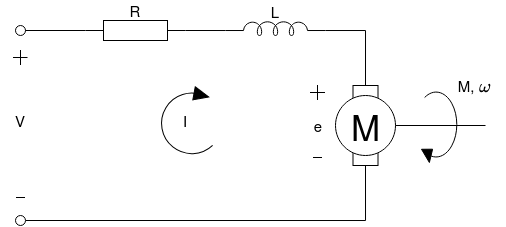
\includegraphics[width=0.6\columnwidth]{images/fundamentos/MotorDC.png} 
    \par\end{centering}

    \label{fig:motordc}
\end{figure}

A figura \ref{fig:motordc} fornece um modelo para o sistema eletromecânico
da armadura de um motor DC, onde uma tensão de entrada, $V$, resulta 
em um torque e velocidade de saída, denominados respectivamente por 
$T$ e $\omega$. A equação elétrica que dita o funcionamento do motor
é expressa em \ref{eq:motordc-eletrico} \cite{krishnan2001electric}.

\begin{equation}
    \label{eq:motordc-eletrico}
    V = e + RI + L \frac{dI}{dt}
\end{equation}

Sabendo que o torque de saída se relaciona com a corrente de entrada
por meio da equação \ref{eq:motordc-torque}, e simplificando a carga
do sistema como um momento de inércia $\mathcal{I}$ e um atrito viscoso, $B$,
obtém-se a equação \ref{eq:motordc-tw} \cite{krishnan2001electric}.

\begin{equation}
    \label{eq:motordc-torque}
    T = K_b I
\end{equation}

\begin{equation}
    \label{eq:motordc-tw}
    T = \mathcal{I}s\omega + B\omega
\end{equation}

Reagrupando as equações de \ref{eq:motordc-eletrico} a \ref{eq:motordc-tw},
é possível observar uma relação entre a velocidade de saída e a tensão
de entrada, ilustrada através da equação \ref{eq:motordc-tf}, no domínio 
de Laplace.

\begin{equation}
    \label{eq:motordc-tf}
    \frac{\omega(s)}{V(s)} = \frac{K_b}{s^2(\mathcal{I}L)+s(BL+\mathcal{I}R)+(BR+K_b^2)}
\end{equation}

A equação em \ref{eq:motordc-tf} fornece um modelo de segunda ordem para
o controle de velocidades de motores DC, entretanto, caso a indutância
do circuito de armadura, $L$, seja desprezível, é possível aproximar 
o modelo proposto como um sistema de primeira ordem.

A fim de controlar a tensão de entrada nestes motores, e consequentemente 
a velocidade de saída, pode-se utilizar um circuito que converta uma tensão
contínua em uma tensão alternada, como através de um circuito do tipo 
\textit{chopper} \cite{krishnan2001electric}.
Circuitos conversores na configuração ponte completa, também conhecidos por 
ponte H completa, ou \textit{Full-H Bridge}, são largamente utilizados na 
geração de níveis de tensão \cite{rashid2017power}, e juntamente com a técnica de controle de 
modulação de largura de pulso - PWM, fornecem um bom meio para controle de 
circuitos análogicos \cite{barr2001pulse}, neste caso, a velocidade, e direção, de um motor DC.

\subsection{Motores de passo}
Motores de passo são, por sua vez, considerados como uma categoria de
motor síncrono, onde a frequência da alimentação que comanda a sua 
velocidade de rotação. Estes motores são utilizados em diversos sistemas
de controle, por oferecem um controle preciso, mesmo em malha 
aberta \cite{chapman2005electric}.  

Embora considerados como máquinas síncronas, os motores de passo são
ativados por uma sequência de chaveamento de suas bobinas que alinham,
a cada passo, o rotor com o campo magnetico gerado no estator. Uma 
relação entre a velocidade de rotação elétrica e a velocidade de rotação do
eixo do motor é proposta em \cite{chapman2005electric} e pode ser vista
na equação \ref{eq:stepper1}, onde $P$ denomina a quantidade de pólos
no motor. 

\begin{equation}
    \label{eq:stepper1}
    \omega_m = \frac{2}{P}\omega_e
\end{equation}

Em \cite{atmel2006stepper}, define-se uma relação mais direta entre 
a velocidade de rotação e o tempo decorrido entre os pulsos enviados por um 
microcontrolador para comando do motor, visível na equação \ref{eq:stepper2}. 
Esta fonte também indica as diferenças básicas entre motores de passo
bipolares e unipolares, bem como no modo de ativação dos motores, com
a possibilidade de uso de configurações de passo completo e meio-passo.

\begin{equation}
    \label{eq:stepper2}
    \omega_m = \frac{\alpha_s}{\delta t} = \frac{\alpha_s}{kt_0}
\end{equation}

Na equação \ref{eq:stepper2}, a constante $\alpha_s$ define o ângulo de passo
básico para determinado motor, ou seja, a variação de rotação na saída 
resultante de um passo na entrada. O termo $\delta t$ informa o período,
em segundos, entre dois pulsos consecutivos para avanço do motor, 
este período pode ser definido como algum múltiplo de um período básico
do microcontrolador, $t_0$, onde somente após decorridos
$k$ períodos internos no controlador, este provocará um pulso para ativação
do motor controlado.

Deste modo, nota-se que o controle de velocidade pode ser realizado
apenas alterando o valor de $k$, através de um contador variável no 
sistema do microcontrolador. Para que motores de passo atinjam determinada
velocidade de uma maneira suave, é necessário que seja realizado um 
controle da aceleração e desaceleração do mesmo, 
variando o valor de $k$ de modo incremental, para que se obtenha uma
rampa de velocidade na saída, com uma aceleração finita \cite{atmel2006stepper}.
Um exemplo de perfil de aceleração pode ser visto na figura \ref{fig:stepperspeed}.

\begin{figure}[h]
    \caption{Exemplo de controle de velocidade para motor de passo.}    

    \begin{centering}
        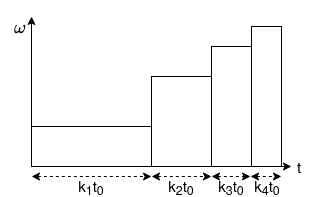
\includegraphics[width=0.5\columnwidth]{images/fundamentos/StepperSpeed.png} 
    \par\end{centering}

    \label{fig:stepperspeed}
\end{figure}

%\subsection{Controle adaptativo}

%\subsection{Controle complacente}

\section{Cinemática de manipuladores}
Um manipulador pode ser analisado como um conjunto de elos conectados
entre si por juntas, e para descrever a relação entre estes elos, 
são definidos sistemas de coordenadas para diferentes partes do 
manipulador, a fim de lidar com a geometrica complexa deste \cite{craig2009introduction}.

Para a correta atribuição de sistemas de coordenadas ao robô, é 
preciso seguir alguma convenção, como aquela definida em \cite{craig2009introduction}.
A convenção apresentada, e que será utilizada ao longo deste trabalho,
define que um sistema de coordenadas será atribuído a cada elo do sistema,
e estes serão numerados de acordo com o elo, onde a base imóvel do robô
é definida como o elo de índice 0. O eixo unitário $\hat{Z}_i$ deve ter a mesma
direção do eixo de rotação do respectivo elo $i$, a origem do sistema 
será posicionada no ponto de intersecção entre o eixo de rotação do elo
um eixo perpendicular a este eixo e o eixo de rotação do próximo elo e o 
eixo $\hat{X}_i$ fica ao longo deste mesmo eixo perpendicular. Por fim, 
o eixo $\hat{Y}_i$ é estabelecido através da regra da mão direita.

Para relacionar matemáticamente os diversos sistemas atribuídos ao 
manipulador, são extraídos parâmetros capazes de relacionar a rotação
e translação entre sistemas de coordenadas consecutivos. Um 
conjunto de parâmetros, utilizado em conjunto com a convenção proposta,
são os parâmetros de Denavit-Hartenberg, ou simplesmente parâmetros de 
DH, em sua forma modificada, estes parâmetros são resumidos do seguinte
modo:

\begin{itemize}
    \begin{centering}
    \item[] $a_i$ = distância entre $\hat{Z}_i$ e $\hat{Z}_{i+1}$, ao longo de $\hat{X}_i$;
    \item[] $\alpha_i$ = ângulo entre $\hat{Z}_i$ e $\hat{Z}_{i+1}$, em relação a $\hat{X}_i$;
    \item[] $d_i$ = distância entre $\hat{X}_{i-1}$ e $\hat{X}_i$, ao longo de $\hat{Z}_i$;
    \item[] $\theta_i$ = ângulo entre $\hat{X}_{i-1}$ e $\hat{X}_i$, em relação a $\hat{Z}_i$.
    \par\end{centering}
\end{itemize}

Percebe-se que para representar a posição e orientação do sistema de 
índice $i$ em relação ao sistema $i-1$, são necessários os parâmetros 
$\alpha_{i-1}$, $a_{i-1}$, $d_i$ e $\theta_i$. 
A equação \ref{eq:transform} ilustra a transformação necessária
para representar um vetor em coordenadas homogêneas definido no 
sistema de coordenadas $i$, em relação ao sistema $i-1$.

\begin{equation}
    \label{eq:transform}
    ^{i-1}_iT = 
    \begin{bmatrix}
        cos\theta_i                 & -sen\theta_i                  & 0                 & a_{i-1}               \\
        sen\theta_icos\alpha_{i-1}  & cos\theta_icos\alpha_{i-1}    & -sen\alpha_{i-1}  & -sen\alpha_{i-1}d_i   \\
        sen\theta_isen\alpha_{i-1}  & cos\theta_isen\alpha_{i-1}    & cos\alpha_{i-1}   & cos\alpha_{i-1}d_i    \\
           0                        &    0                          &    0              &  1                    \\    
    \end{bmatrix}
\end{equation}

A transformação exposta em \ref{eq:transform} é composta pela junção
de uma matriz de rotação, $^{i-1}_iRot$, um vetor de translação, $^{i-1}Pos_i$,
e uma linha extra composta por três zeros e um único um,
a fim de transformar a matriz em uma matriz quadrátrica, facilitando
a inversão da transformação, como indicado na equação \ref{eq:transform2}. 

\begin{equation}
    \label{eq:transform2}
    ^{i-1}_iT = 
    \begin{bmatrix}
        ^{i-1}_iRot & ^{i-1}Pos_i   \\
        0 \;\; 0 \;\; 0       & 1   \\
    \end{bmatrix}
\end{equation}

A notação adotada para os índices 
sobrescritos e subescritos se manterá a mesma ao longo de todo este
documento, onde o índice sobrescrito precedente denota o sistema de 
coordenadas de referência de referência desejado, e o índice subescrito 
precedente informa o sistema de coordenadas original.

\subsection{Propagação de velocidades}
É possível definir a velocidade angular e linear de determinado 
sistema de referência no manipulador em função da movimentação desta
junta e da movimentação de juntas passadas. Através dos cálculos 
desenvolvidos em \cite{craig2009introduction}, são obtidas 
equações para a propagação de velocidades entre juntas, referenciadas
nas equações \ref{eq:speed1} e \ref{eq:speed2}.

\begin{equation}
    \label{eq:speed1}
    ^{i+1}\omega_{i+1} = \; ^{i+1}_iRot\,^i\omega_i + \dot{\theta}_{i+1}\,^{i+1}\hat{Z}_{i+1}
\end{equation}

\begin{equation}
    \label{eq:speed2}
    ^{i+1}v_{i+1} = \; ^{i+1}_iRot\left(^iv_i+^i\omega_i\times ^iPos_{i+1}\right)
\end{equation}

As equações \ref{eq:speed1} e \ref{eq:speed2} dizem respeito à velocidades
geradas por juntas de rotação. A velocidade angular pode ser vista 
como uma soma entre a velocidade angular da junta precedente, 
termo $^{i+1}_iRot\,^i\omega_i$, e a rotação gerada pelo próprio eixo,
$\dot{\theta}_{i+1}\,^{i+1}\hat{Z}_{i+1}$. 
A velocidade linear, por sua vez, é a soma da velocidade linear da 
junta precedente com a resultante linear da multiplicação vetorial
entre a velocidade angular da junta precedente com o deslocamento, 
ambos representados no novo sistema de coordenadas, $i+1$.

\subsection{Jacobiana}
\label{sec:jacobiana}

Aplicando-se as equações \ref{eq:speed1} e \ref{eq:speed2} para as juntas
de um manipulador, é possível obter as velocidades de cada elo em função
dos termos $\dot{\theta}_i$, agrupando-se estas relações em uma forma matricial,
gera-se uma representação entre as velocidades das juntas e as velocidades
lineares e angulares de diversos elos. À matriz resultante deste 
agrupamento, que relaciona variações temporais na entrada com 
a saída, relação visível na equação \ref{eq:mjacobiana}, atribui-se o 
nome de Jacobiana \cite{craig2009introduction}.

\begin{equation}
    \label{eq:mjacobiana}
    \dot{Y} = J(X)\dot{X}
\end{equation}

Em certos casos, a matriz Jacobiana pode ser organizada com a sua 
inversão em mente, para que se obtenha a velocidade que deve ser 
imposta nas juntas de um robô para gerar determinadas velocidades
lineares e angulares desejadas.

\begin{comment}
Desenvolvimentos
\end{comment}
\chapter{Modelagem}

O primeiro sistema de coordenadas a ser posicionado foi o da junta 1. Através da figura \ref{fig:a1}
nota-se que os eixos das juntas 1 e 2 não se interceptam, portanto a origem foi posicionada no ponto 
de intersecção entre a perpendicular comum e o eixo da junta 1, equivalente ao quadrado verde na figura. 
O eixo $\hat{Z}_1$ foi posicionado na direção do eixo da junta $1$, com sentido para fora do plano da imagem,
e o eixo $\hat{X}_1$ na direção da perpendicular comum, com sentido do eixo da junta 1 para o eixo da junta 2.
Na figura a distância mostrada faz referência ao parâmetro $a_1$.

\begin{figure}[ht]
    \caption{Distância entre os eixos das juntas 1 e 2.}    
    \begin{centering}

        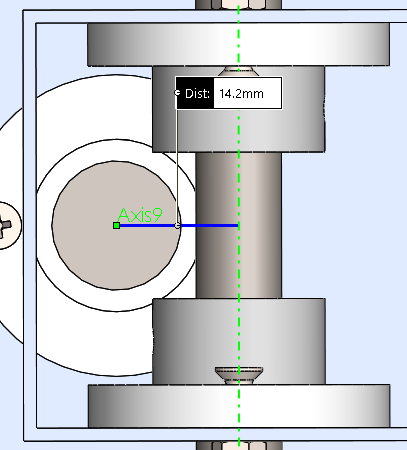
\includegraphics[width=0.5\columnwidth]{images/a1.png}
    
    \par\end{centering}

    \label{fig:a1}
\end{figure}

Seguindo os passos de 2 a 5 descritos na seção \ref{sec:fundamentos} foram definidos também os sistemas
de coordenadas das juntas de 2 a 5, resultando nos parâmetros $a_2$, $a_3$ e $a_4$. Os valores para estes
termos podem ser vistos nas figuras de \ref{fig:a2} a \ref{fig:a4}. 
Vale a pena notar que para a junta 5, os eixos $\hat{Z}_5$ e $\hat{Z}_6$ se interceptam, como pode ser
visto na figura \ref{fig:d6}, portanto o eixo $\hat{X}_5$ foi definido na direção da reta normal ao plano 
formado por esses dois eixos $\hat{Z}$.  

\begin{figure}[ht]
    \caption{Distância entre os eixos das juntas 2 e 3.}    
    \begin{centering}

        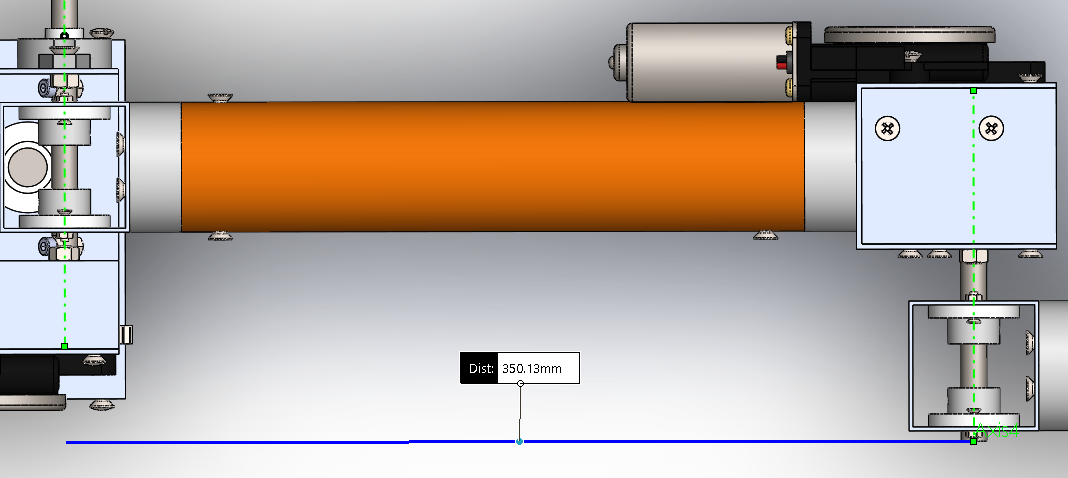
\includegraphics[width=1\columnwidth]{images/a2.png}
    
    \par\end{centering}

    \label{fig:a2}
\end{figure}

\begin{figure}[ht]
    \caption{Distância entre os eixos das juntas 3 e 4.}    
    \begin{centering}

        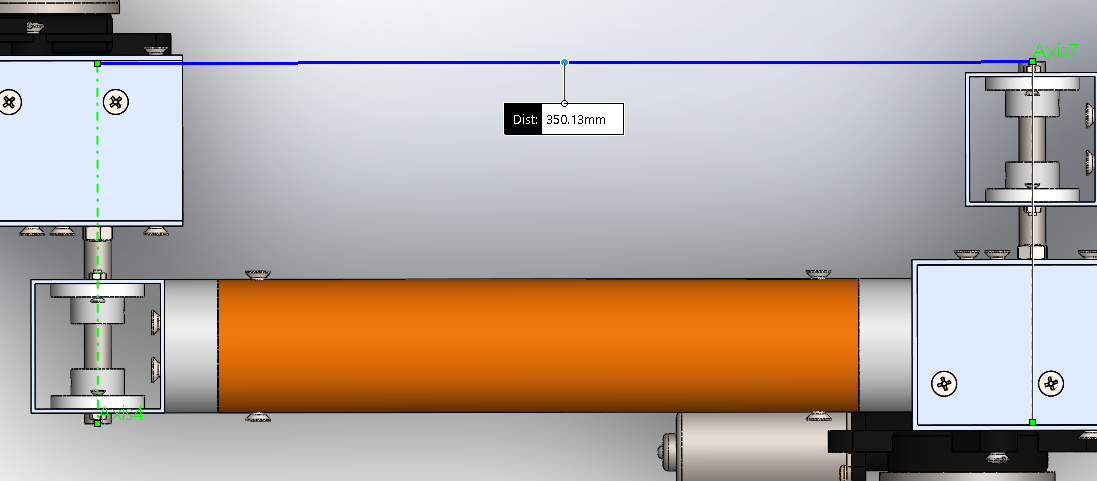
\includegraphics[width=1\columnwidth]{images/a3.png}
    
    \par\end{centering}

    \label{fig:a3}
\end{figure}

\begin{figure}[ht]
    \caption{Distância entre os eixos das juntas 4 e 5.}    
    \begin{centering}

        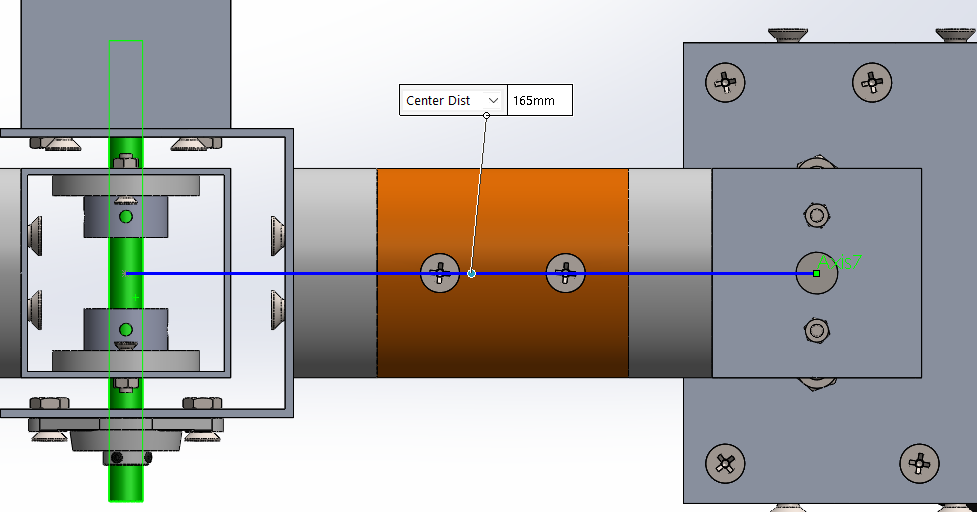
\includegraphics[width=0.9\columnwidth]{images/a4.png}
    
    \par\end{centering}

    \label{fig:a4}
\end{figure}

Para o sistema de coornadas da base, $\{0\}$, optou-se por posicionar este a uma distância $d_1$ do sistema ${1}$, 
por acreditar que isto facilitaria uma transformação entre a base do sistema e um sistema de referência global
da estação de uso real do manipulador. 
Como é definido em \cite{craig2009introduction}, a posição deste sistema é arbitrário, portanto
esta decisão não fere a convenção adotada.

Para a junta 6, a origem do sistema foi posicionada no centro do eixo de saída do manipulador empregado nesta 
junta, assumindo que esta decisão tornaria mais simples uma definição da transformação entre a ferramenta a 
ser utilizada no manipulador e a última junta do sistema. Esta decisão resultou em um parâmetro $d_6$, que 
indica a distância entre $\hat{X}_5$ e $\hat{X}_6$ ao longo de $\hat{Z}_6$, respeitando a convenção adotada.
O valor deste parâmetro pode ser visto na figura \ref{fig:d6}.

\begin{figure}[ht]
    \caption{Distância entre o eixo da junta 5 e a origem do sistema da junta 6.}    
    \begin{centering}

        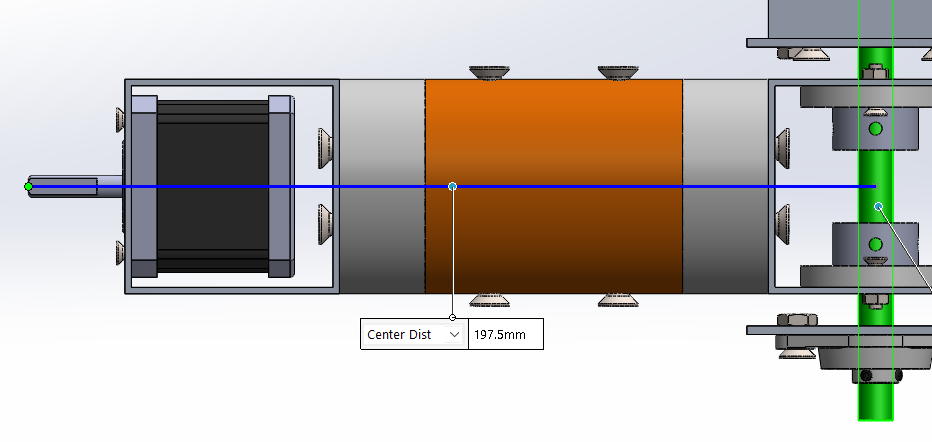
\includegraphics[width=0.9\columnwidth]{images/d6.png}
    
    \par\end{centering}

    \label{fig:d6}
\end{figure}

\begin{comment}
Continuação desenvolvimentos.
\end{comment}
%\chapter{Projeto Sistema de Controle}

% Notas:
%   Eixos x, y e z utilizados como equações. ex: $x$, $y$ e $z$.

\label{CapProjCont}

% Resumo opcional. Comentar se não usar.
%\resumodocapitulo{Resumo opcional}

\section{Modelagem}
Para o desenvolvimento de um sistema de controle é interessante inicialmente
definir o modelo deste, identificando variáveis importantes para o sistema,
como variáveis de entrada, de saída, e variáveis controladas.

O manipulador em questão será controlado por um \textit{joystick}, 
que implementa a interface entre o sistema de controle e o usuário. 
Consequentemente, define-se como variáveis de entrada os valores 
dos eixos $x$, $y$ e $z$ lidos através do \textit{joystick}.

O efetuador final do braço robótico é o que realizará de fato a
interface entre o usuário e o ambiente, deste modo, é interessante
que o usuário tenha controle sobre à localização 3D do efetuador
no espaço e sua orientação, resultando em 6 variáveis de saída desejadas.

Como há somente 3 variáveis de entrada para controle das 6 variáveis de 
interesse, optou-se por dividir o volume de trabalho do manipulador em 
planos. Ao todo, foram criados 4 planos de ação, 2 planos de translação, 
$XY$ e $XZ$, e 2 planos de rotação, $R1$ e $R2$. Os planos de translação
fazem referência ao sistema de coordenadas global, afixado à base do 
manipulador. Já os planos de rotação foram afixados à quinta junta do manipulador, 
adotando-se que o ser humano consegue interpretar mais facilmente a rotação 
de um objeto em torno do seu próprio eixo do que em termos de rotação nos 
eixos do sistema de coordenadas global, facilitando o controle do pulso do manipulador. 

Esta organização de sub-planos de trabalho foi realizada de modo a facilitar 
o entendimento pelo usuário. Para cada plano de ação, 2 das variáveis de entrada 
serão relacionadas com as variáveis pertinentes a cada plano, alternando-se entre 
os planos de ação por meio da terceira entrada do \textit{joystick}. As variáveis dos
planos de translação estão indicas no nome do próprio plano, $XY$ ou $XZ$. Para os planos
de rotação, foram utilizados como base os eixos $\hat{Y}_5$ e $\hat{Z}_5$ para o plano
$R1$ e os eixos $\hat{Y}_5$ e $\hat{X}_5$ para o plano $R2$. Uma rotação em torno do eixo 
$\hat{Y}_5$ gera a mesma rotação em torno do eixo $\hat{Z}_6$, controlando diretamente 
a rotação do punho. Já o eixo $\hat{Z}_5$ controla a guinada, e por fim, o eixo $\hat{X}_5$
se relaciona com a arfagem, finalizando as 3 movimentações possíveis para o punho.

É necessário definir também a interação entre os dados de entrada do usuário e 
as variáveis internas do robô. Pela imensa quantidade de posições e orientações possíveis, 
adotou-se que os \textit{inputs} do usuário, limitados a dois eixos, não poderiam ser diretamente relacionados
com posições, mas sim com um desejo de movimento do robô controlado. Portanto, 
os dados lidos pelo \textit{joystick} serão transformados em velocidades a serem impostas
no efetuador final, sejam estas de translação ou rotação, a depender do plano de ação.

\section{Análise Cinemática}
\label{sec:analise-cinematica}

Como informado na seção \ref{sec:jacobiana} deste documento, a jacobiana
é uma matriz que relaciona as diversas velocidades em um manipulador 
robótico, podendo ser utilizada para representar a velocidade do efetuador final
em função da velocidade de variação dos ângulos das juntas.
Para se obter então esta relação é necessário seguir as equações de propagação
de velocidades no manipulador, \ref{eq:speed1} e \ref{eq:speed2}.
Estas equações dependem das matrizes de rotação e translação entre as 
juntas, que podem ser encontradas utilizando as regras dispostas nas 
equações \ref{eq:transform} e \ref{eq:transform2}.

Utilizando os parâmetros de DH do novo modelo, dispostos na tabela \ref{tab:DH-comparacao},
e a equação \ref{eq:transform}, foram obtidas as matrizes $^{i-1}_iT$, para $i$ de 1 a 6. 
Os resultados obtidos estão dispostos nas equações de \ref{eq:t01} a \ref{eq:t56}.
Para facilitar o entendimento, as funções trigonométricas seno e cosseno serão abreviadas pelas
letras $s$ e $c$, respectivamente.

\begin{multicols}{2}
    \noindent
    \begin{equation}
        \label{eq:t01}
        ^0_1T = \begin{bmatrix}
                    c\theta_1 & -s\theta_1 & 0 & 0 \\
                    s\theta_1 & c\theta_1 & 0 & 0 \\
                    0 & 0 & 1 & d_1 \\
                    0 & 0 & 0 & 1 \\
                \end{bmatrix}
    \end{equation}
    \begin{equation}
        ^1_2T = \begin{bmatrix}
                    c\theta_2 & -s\theta_2 & 0 & a_1 \\
                    0 & 0 & -1 & 0 \\
                    s\theta_2 & c\theta_2 & 0 & 0 \\
                    0 & 0 & 0 & 1 \\
                \end{bmatrix}
    \end{equation}
\end{multicols}

\begin{multicols}{2}
    \noindent
    \begin{equation}
        ^2_3T = \begin{bmatrix}
                    c\theta_3 & -s\theta_3 & 0 & a_2 \\
                    s\theta_3 & c\theta_3 & 0 & 0 \\
                    0 & 0 & 1 & 0 \\
                    0 & 0 & 0 & 1 \\
                \end{bmatrix}
    \end{equation}
    \begin{equation}
        ^3_4T = \begin{bmatrix}
                    c\theta_4 & -s\theta_4 & 0 & a_3 \\
                    s\theta_4 & c\theta_4 & 0 & 0 \\
                    0 & 0 & 1 & 0 \\
                    0 & 0 & 0 & 1 \\
                \end{bmatrix}
    \end{equation}
\end{multicols}

\begin{multicols}{2}
    \noindent
    \begin{equation}
        \label{eq:t45}
        ^4_5T = \begin{bmatrix}
                    s\theta_5' & c\theta_5' & 0 & a_4 \\
                    0 & 0 & -1 & 0 \\
                    -c\theta_5' & s\theta_5' & 0 & 0 \\
                    0 & 0 & 0 & 1 \\        
                \end{bmatrix}
    \end{equation}
    \begin{equation}
        \label{eq:t56}
        ^5_6T = \begin{bmatrix}
                    c\theta_6 & -s\theta_6 & 0 & 0 \\
                    0 & 0 & 1 & d_6 \\
                    -s\theta_6 & -c\theta_6 & 0 & 0 \\
                    0 & 0 & 0 & 1 \\
                \end{bmatrix}
    \end{equation}
\end{multicols}

Nota-se que para a transformação da equação \ref{eq:t45} utilizou-se a nova variável
$\theta_5'$, de acordo com a equação \ref{eq:junta5-offset}.

A transformação de um vetor expresso no sistema da última junta do punho para coordenadas
globais, ou seja, para o sistema de coordenadas da base, foi obtida através 
da multiplicação de todas as transformações, de maneira consecutiva, como indicado na
equação \ref{eq:t06}.
Esta transformação é importante para referenciar as velocidades
da ponta do manipulador para o sistema global, de mais fácil visualização e entendimento
por parte de usuários.

\begin{equation}
    \label{eq:t06}
    ^0_6T = ^B_6T = ^0_1T*^1_2T*^2_3T*^3_4T*^4_5T*^5_6T
\end{equation}

Aplicando-se então as equações \ref{eq:speed1} e \ref{eq:speed2}, e utilizando para a 
base vetores nulos de velocidades, isto é, $^0\omega_0 = \, ^0v_0 = \left[0 \; 0 \; 0 \right]^T$,
foram obtidas as velocidades lineares e angulares de todas as juntas, expressas nos seus devidos 
sistemas de coordenadas. As velocidades de interesse a serem controladas pelo usuário, ou seja,
as velocidades do final do manipulador, $\omega_6$ e $v_6$, foram remetidas ao sistema de 
coordenadas da base pré-multiplicando os vetores $^6\omega_6$ e $^6v_6$ pela matrix $^0_6Rot$,
que compõe parte da matriz $^0_6T$, previamente calculada.
Os resultados obtidos para esses dois vetores de velocidade estão dispostos nas equações 
\ref{eq:0w6} e \ref{eq:0v6}.

\begin{equation}
    \label{eq:0w6}
\begin{gathered}
    ^0\omega_6 = \begin{bmatrix}
        s\theta_1(\dot{\theta}_2 + \dot{\theta}_3 + \dot{\theta}_4) + c\theta_1s(\theta_2+\theta_3+\theta_4)\dot{\theta}_5 + \\
        + [c\theta_1c\theta_5'c(\theta_2+\theta_3+\theta_4) +s\theta_1s\theta_5']\dot{\theta}_6\\
        \\
        -c\theta_1(\dot{\theta}_2+\dot{\theta}_3+\dot{\theta}_4) + s\theta_1s(\theta_2+\theta_3+\theta_4)\dot{\theta}_5 + \\
        +[s\theta_1c\theta_5'c(\theta_2+\theta_3+\theta_4) -c\theta_1s\theta_5']\dot{\theta}_6 \\
        \\
        \dot{\theta}_1 -c(\theta_2+\theta_3+\theta_4)\dot{\theta}_5 + \\
        +c\theta_5's(\theta_2+\theta_3+\theta_4)\dot{\theta}_6 \\   
    \end{bmatrix}
\end{gathered}
\end{equation}

\begin{equation}
    \label{eq:0v6}
\begin{gathered}
    ^0v_6 = 
    \begin{bmatrix}
        % First line
        \{c\theta_1s\theta_5'd_6 - s\theta_1[a_1 + c\theta_2a_2 + c(\theta_2 + \theta_3)a_3 + c(\theta_2+\theta_3+\theta_4)(a_4 + c\theta_5'd_6)]\}.\dot{\theta}_1 - \\
        - c\theta_1[s\theta_2a_2 + s(\theta_2 + \theta_3)a_3 + s(\theta_2+\theta_3+\theta_4)(a_4 + c\theta_5'd_6)].\dot{\theta}_2 - \\
        - c\theta_1[s(\theta_2+\theta_3)a_3 + s(\theta_2+\theta_3+\theta_4)(a_4 + c\theta_5'd_6)].\dot{\theta}_3 - \\
        - c\theta_1s(\theta_2+\theta_3+\theta_4)(a_4 + c\theta_5'd_6).\dot{\theta}_4 + \\
        + [c\theta_1s\theta_5'c(\theta_2+\theta_3+\theta_4) - s\theta_1c\theta_5']d_6.\dot{\theta}_5 \\
        \\

        % Second line
        \{s\theta_1s\theta_5'd_6 + c\theta_1[a_1 + c\theta_2a_2 + c(\theta_2+\theta_3)a_3 + c(\theta_2 + \theta_3 + \theta_4)(a_4 + c\theta_5'd_6)]\}.\dot{\theta}_1 - \\
        -s\theta_1[s\theta_2a_2 + s(\theta_2+\theta_3)a_3 + s(\theta_2+\theta_3+\theta_4)(a_4 + c\theta_5'd_6)].\dot{\theta}_2 - \\
        -s\theta_1[s(\theta_2+\theta_3)a_3 + s(\theta_2+\theta_3+\theta_4)(a_4 + c\theta_5'd_6)].\dot{\theta}_3 - \\
        -s\theta_1s(\theta_2+\theta_3+\theta_4)(a_4 + c\theta_5'd_6).\dot{\theta}_4 + \\
        +[s\theta_1s\theta_5'c(\theta_2+\theta_3+\theta_4) + c\theta_1c\theta_5']d_6.\dot{\theta}_5\\
        \\

        % Third line
        [c\theta_2a_2 + c(\theta_2+\theta_3)a_3 + c(\theta_2+\theta_3+\theta_4)(a_4 + c\theta_5'd_6)].\dot{\theta}_2 + \\
        +[c(\theta_2+\theta_3)a_3 + c(\theta_2+\theta_3+\theta_4)(a_4+c\theta_5'd_6)].\dot{\theta}_3 + \\
        +c(\theta_2+\theta_3+\theta_4)(a_4+c\theta_5'd_6).\dot{\theta}_4 + \\
        +s\theta_5's(\theta_2+\theta_3+\theta_4)d_6.\dot{\theta}_5\\
    \end{bmatrix}
\end{gathered}
\end{equation}

Analisando a equação \ref{eq:mjacobiana} e sabendo que o vetor de velocidade das juntas
é um vetor coluna 6x1, $\dot{\Theta} = [\dot{\theta}_1 \; \dot{\theta}_2 \; \dot{\theta}_3 \; \dot{\theta}_4 \; \dot{\theta}_5 \; \dot{\theta}_6]^T$,
é possível escrever um vetor de velocidades do efetuador final como a junção dos vetores de velocidade linear
e angular, para obter uma matriz jacobiana quadrada, passível de ser invertida para que as velocidades das juntas
sejam representadas em função da velocidade desejada do manipulador final. Estas relações estão dispostas nas equações 
\ref{eq:jac1} e \ref{eq:jac2}.

\begin{multicols}{2}
    \noindent
    \begin{equation}
        \label{eq:jac1}
        ^0\nu = \begin{bmatrix}
                    ^0v_6 \\
                    ^0\omega_6
                \end{bmatrix}
              = \,^0\!J(\Theta)\dot{\Theta}
    \end{equation}
    \noindent
    \begin{equation}
        \label{eq:jac2}
        \dot{\Theta} = \,^0\!J^{-1}(\Theta)^0\nu = \,^0\!J^{-1}(\Theta)\begin{bmatrix}
                                                                            ^0v_6 \\
                                                                            ^0\omega_6
                                                                        \end{bmatrix}
    \end{equation}
\end{multicols}

Os termos da jacobiana podem ser obtidos através de análise das equações \ref{eq:0w6} e \ref{eq:0v6},
sendo os termos que multiplicam as derivadas dos ângulos das juntas.

Buscando-se evitar gasto excessivo de processamento na inversão desta matriz jacobiana 6x6 para cada
novo valor do vetor $\Theta$, foi realizada uma inversão simbólica da matriz, isto é, mantendo os 
valores de $\theta_1$ a $\theta_6$ como variáveis. Para inverter a matriz jacobiana foi utilizado o 
método de inversão por matriz adjunta. A equação base que rege este método está disposta em \ref{eq:inv_adjunta}.

\begin{equation}
    \label{eq:inv_adjunta}
    J^{-1}  = \frac{1}{|J|}.adj(J)
\end{equation}

Nota-se pela equação \ref{eq:inv_adjunta} que para a inversão são necessários o determinante da matriz,
identificado por $|J|$, e sua matriz adjunta. O determinante da matriz foi calculado e o resultado obtido
está definido na equação \ref{eq:det}.

\begin{equation}
    \label{eq:det}
    |J| = -c\theta_5's\theta_3a_2a_3[a_1+c\theta_2a_2+c(\theta_2+\theta_3)a_4+c(\theta_2+\theta_3+\theta_4)(a_4+2c\theta_5'd_6)]  
\end{equation}

A matriz adjunta foi então calculada a partir dos cofatores da matriz, finalizando o 
processo de inversão. 
A matriz resultante obtida foi comparada com a matriz invertida a partir dos \textit{softwares}
\textit{MATLAB} e \textit{Maple}, próprios para cálculos algébricos, verificado-se que o 
resultado obtido a partir dos cálculos manuais estava correto.

Foi escrita então uma rotina na linguagem ``c++'' que realiza a inversão da 
matriz, calculando os cofatores e determinante a partir de seus termos simbólicos. 
Visando reduzir a quantidade de cálculos a serem realizados pelo controlador, os termos da 
matriz jacobiana inversa foram reagrupados, favorecendo o reúso de variáveis.
Para verificar a rotina criada, foi escrito um \textit{script} em \textit{python}
que realizava as equações \ref{eq:jac1} e \ref{eq:jac2} em sequência, para uma 
determinada configuração de ângulos e suas velocidades, obtendo uma velocidade para 
a última junta e então realizando o processo inverso pelo uso da rotina criada, esperando-se 
obter os mesmos valores iniciais.

\section{Tratamento das variáveis de entrada}
As variáveis de entrada do sistema serão dois valores de ângulos impostos pelo
usuário ao \textit{joystick}. Para transformar estes dados em uma indicação de 
velocidade, foi necessário inicialmente realizar uma calibração dos valores lidos.
Para realizar a calibração, criou-se uma rotina que no início do sistema 
realiza uma quantidade fixa de medidas destes valores, e define um valor médio para
cada eixo, com base na média destas leituras. Para valores próximos a este valor médio,
assume-se ausência de movimento.

Para transformar os dados de leitura do \textit{joystick} em um vetor indicando
a velocidade desejada no plano de atuação do sistema, foi necessário transformar
a área efetiva de movimentação conjunta dos potenciômetros do \textit{joystick},
inicialmente um quadrado, em um círculo, com módulo máximo igual a 100\%.
Este mapeamento para uma nova área efetiva é necessário para 
garantir que todas as posições do \textit{joystick} estarão sujeitas às mesmas 
limitações de módulo, o que não é verdade para uma área em formato quadrado.

Para realizar esta transformação, é calculado o ângulo em que o \textit{joystick}
se encontra através dos valores dos eixos $x$ e $y$, é então calculado o módulo máximo 
passível de ser obtido com esse ângulo. Os novos valores de $x$ e $y$ são posteriormente
definidos com base na relação entre o módulo real do sensor e o módulo máximo, e no 
ângulo observado.

\section{Motores de passo}

Para o controle da velocidade dos motores de passo utilizou-se como base a equação
\ref{eq:stepper2}. Buscando-se definir rampas de aceleração para o acionamento
desses motores e consequentemente maior suavidade no movimento, foi formulada a equação 
\ref{eq:stepper3}.

\begin{equation}
    \label{eq:stepper3}
    \dot{\omega} = \frac{\omega_{i+1}-\omega_i}{k_{i+1}t_0}
\end{equation}

Substituindo a equação \ref{eq:stepper2} para a variável $\omega_{i+1}$
obtém-se a equação de segundo grau \ref{eq:stepper4}, que relaciona o novo 
contador $k_{i+1}$ e a velocidade atual $\omega_i$.

\begin{equation}
    \label{eq:stepper4}
    (k_{i+1}t_0)^2\dot{\omega} = \alpha_s - \omega_ik_{i+1}t_0
\end{equation}

Pela fórmula de Bhaskara, pode-se expressar o novo valor do contador completamente
em função da velocidade atual, para uma aceleração $\dot{\omega}$ definida. Esta 
solução pode ser vista na equação \ref{eq:stepper5}. A solução com valor negativo
para o resultado da raiz quadrada foi ignorada, por resultar sempre em um valor negativo,
impossível de ser atribuído a um contador.

\begin{equation}
    \label{eq:stepper5}
    k_{i+1} = \frac{-\omega_i + \sqrt{\omega_i^2+4\dot{\omega}\alpha_s}}{2t_0\dot{\omega}}
\end{equation}

Como informado na seção do controlador empregado, e seguindo a tabela \ref{tab:Pinout}, os 
pinos que geram os passos destes motores estão conectados a pinos no controlador capazes de 
gerar ondas na saída através de contadores. Dessa maneira, ao se definir uma nova 
velocidade para este tipo de motor, atribuí-se um novo valor para o registrador utilizado 
como comparador na geração destas ondas, seguindo a equação \ref{eq:stepper5}, quando for
detectado uma combinação entre um contador do sistema e o valor configurado, uma sub-rotina
será chamada que alterará o valor do pino definido como saída.

Como os motores de passo não possuem sensores para conhecimento da posição absoluta,
foi definido um momento de calibração para estes motores. No momento de início do programa, 
todos os motores de passo serão acionados com uma certa velocidade até atingir algum sensor 
fim-de-curso, que permite assumir uma posição inicial bem definida para as juntas onde estes
atuadores são empregados. A posição inicial assumida para os três motores de passo do sistema
foram: 

\begin{itemize}
    \item Junta 1: $\pi/2$ rad;
    \item Junta 5: $-\pi/2$ rad;
    \item Junta 6: $0$ rad.
\end{itemize}

\section{Motores DC}

Para controle dos motores DC, foi utilizada uma interrupção periódica no sistema do controlador,
semelhante aos pulsos gerados nos motores de passo, para atualizar o valor de tensão enviada
ao motor. 

Inicialmente, adotou-se uma relação direta entre o ciclo de trabalho de sinais PWM enviados 
ao \textit{driver} do motor e a velocidade de saída, baseando-se no regime permanente 
que seria obtido seguindo a equação \ref{eq:motordc-tf}. Desse modo, para cada motor
DC do sistema, quando a interrupção é gerada, o valor de PWM enviado ao motor é atualizado
multiplicando a velocidade desejada por uma constante, definida empiricamente para cada motor.

Também foi necessário se atentar para os funcionamentos não-lineares apresentados pelos motores
DC, especialmente os valores da zona morta dos motores. Desse modo, caso o valor obtido para
o \textit{duty cycle} esteja abaixo de um certo limiar, o valor será atualizado para este limiar.

Para aprimorar o controle dos motores DC, a função chamada quando da ocorrência da 
interrupção programada no sistema pode ser preparada para operar como parte de um sistema
de controle digital, após devidamente identificados os parâmetros de funcionamento dos
motores.

\section{Fluxograma de operação}

O código principal do sistema de controle foi dividido em sub-rotinas bem definidas, que
em conjunto promovem a movimentação e/ou simulação do sistema robótico. Uma ilustração das
etapas do sistema de controle pode ser vista na figura \ref{fig:fluxograma}.

\begin{figure}[h]
    \caption{Fluxograma do sistema de controle.}

    \begin{centering}
        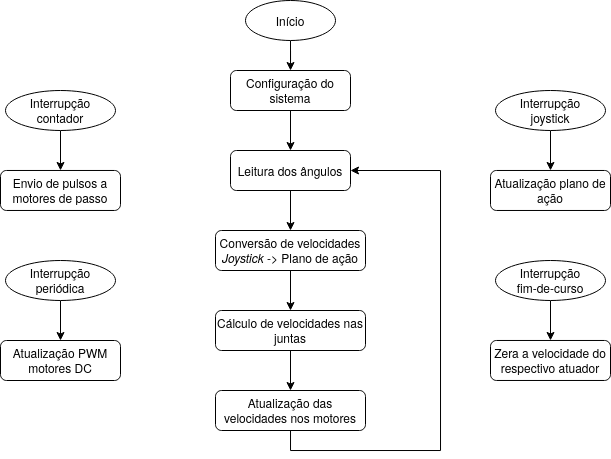
\includegraphics[width=0.7\columnwidth]{images/controle/fluxo.png} 
    \par\end{centering}

    \label{fig:fluxograma}
\end{figure}

Os símbolos ovais indicam as fontes de chamadas a sub-rotinas do código, sendo a fonte 
de início principal, a alimentação do sistema. Assim que é energizado, o sistema é iniciado, sendo
então configurado. Para a definição e configuração do sistema manipulador, foram criadas 
bibliotecas que permitem descrever um manipulador robótico e os atuadores empregados de maneira 
intuitiva e genérica, facilitando o entendimento e modificação do código, através da aplicação de 
técnicas de programação orientada a objetos. Durante a configuração os diversos equipamentos do sistema
serão calibrados e preparados para amplo funcionamento.

As outras fontes de chamadas a sub-rotinas são as interrupções, tanto aquelas geradas pelos contadores
dos motores de passo, quantos as interrupções geradas periodicamente para controle dos motores DC e 
as interrupções geradas por sensores do sistema, como fim de curso ou pelo terceiro eixo do \textit{joystick}. 
Estas interrupções são iniciadas e preparadas no momento de configuração do sistema.

Após a configuração geral do sistema, o laço de repetição principal do sistema é iniciado. 
A primeira tarefa a ser realizada é a leitura de todos os ângulos do sistema, para conhecimento
do estado geral do robô. Após a leitura dos ângulos, são lidos os dados de entrada provindos do 
usuário, e estes valores são então convertidos para as variáveis pertinentes a um dos 4 planos de
ação definidos para o sistema.
Caso o plano de ação 
atual seja um plano de rotação, assume-se que as velocidades indicadas estão representadas no
plano de coordenadas da junta 5, portanto, são transportadas para o eixo de coordenadas da base
por uma pré-multiplicação pela matriz $^0_5Rot$.

Na etapa de cálculo da velocidade nas juntas o vetor de velocidades gerado na etapa anterior será 
transformado para velocidades a serem impressas nos atuadores do sistema, através de chamada
à sub-rotina que implementa a matriz jacobiana inversa do sistema.

A etapa de atualização das velocidades nos motores realizará de fato chamadas à métodos
dos objetos que representam os atuadores do sistema para configurar a estes uma nova referência 
para sua velocidade de rotação. A manutenção desta velocidade será função das sub-rotinas 
chamadas pelas interrupções.

\section{Simulação}

Para verificar o correto funcionamento do sistema de controle, independente dos circuitos de
sensoriamento e acionamento, foi implementada uma função que simula os ângulos de leitura do sistema. 
Para utilização desta função é suficiente alterar no código fonte do programa uma diretiva
definitada como ``\textit{SIMULATION}'' para o valor 1.
Esta função atualiza os valores de ângulos do sistema com base na velocidade a ser imposta nos atuadores
e a quantidade de tempo decorrente durante a execução do laço de repetição principal. 

Com o objetivo de informar estes ângulos a um ambiente externo, foi criada outra rotina que envia os dados 
dos ângulos, lidos e/ou simulados, para algum dispositivo conectado através de uma conexão serial.

Para obtenção dos ângulos e simulação do manipulador de forma visual, o módulo criado para a 
realização das equações de Newton-Euler foi modificado para permitir o desenho do manipulador
na tela de um computador. Foi então codificada uma interface que realiza a comunicação entre o 
sistema na placa controladora Arduino e o módulo em \textit{python} modificado.

Com a possibilidade de simulação e função de comunicação com módulo de simulação, o 
novo fluxograma de controle pode ser visto na figura \ref{fig:fluxograma2}. 

\begin{figure}[h]
    \caption{Fluxograma do sistema de controle com simulação.}

    \begin{centering}
        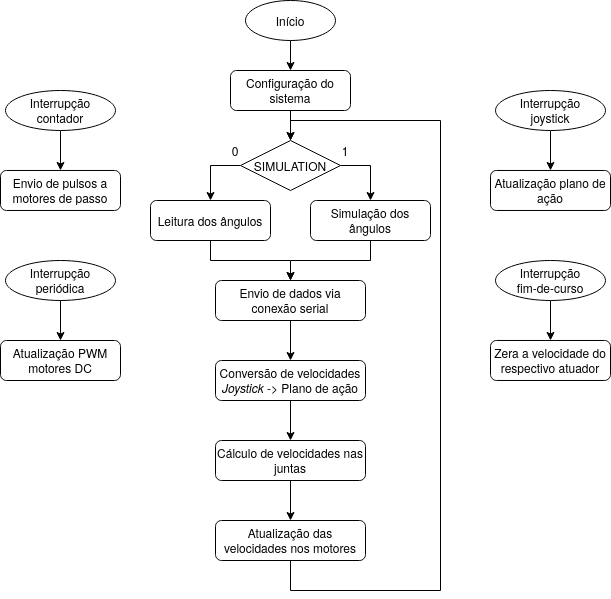
\includegraphics[width=0.7\columnwidth]{images/controle/fluxo2.png} 
    \par\end{centering}

    \label{fig:fluxograma2}
\end{figure}

O ambiente de simulação gerado realiza a animação do manipulador em tempo real, com os dados advindos
do Arduino. Este se mostrou eficiente na reprodução dos movimentos do robô quando não
foi possível utilizar a estrutura mecânica real deste para testes e validação dos circuitos. 
O módulo responsável pela animação foi projetado e codificado de maneira responsiva a mudanças, 
modificando automaticamente as escalas dos três eixos para otimizar o espaço de visualização do robô.

Um exemplo de simulação utilizando o ambiente pode ser visto em \ref{fig:exemplo}, onde foi montado 
um robô genérico com 6 graus de liberdade. As linhas em preto indicam uma conexão direta entre os sistemas 
de referência, e não necessariamente os elos do manipulador.

\begin{figure}[h]
    \caption{Exemplo de robô criado no \textit{software} simulador.}

    \begin{centering}
        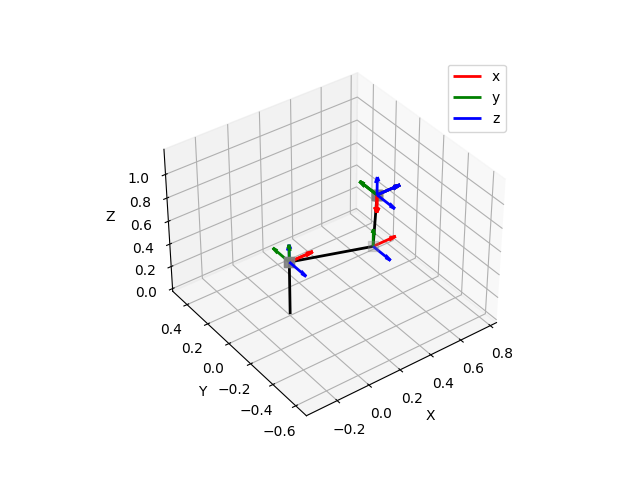
\includegraphics[width=0.8\columnwidth]{images/controle/simu-puma.png} 
    \par\end{centering}

    \label{fig:exemplo}
\end{figure}

\begin{comment}
Resultados
\end{comment}
%\chapter{Resultados}

\label{CapResultados}

\section{Precisão do potenciômetro}
A figura \ref{fig:result-resolution} ilustra o ambiente de testes montado para os
testes de resolução do potenciômetro escolhido. Os dados do potenciômetros eram 
enviados a uma placa de prototipagem que implementa uma versão do circuito
de sensoriamento proposto. Para o teste, os dados do arduino foram lidos de 
maneira bruta, o que para um ADC de 10 bits corresponde a valores entre 0 e 1024.

\begin{figure}[h]
    \caption{Ambiente de testes para medida de resolução do sensor.}

    \begin{centering}
        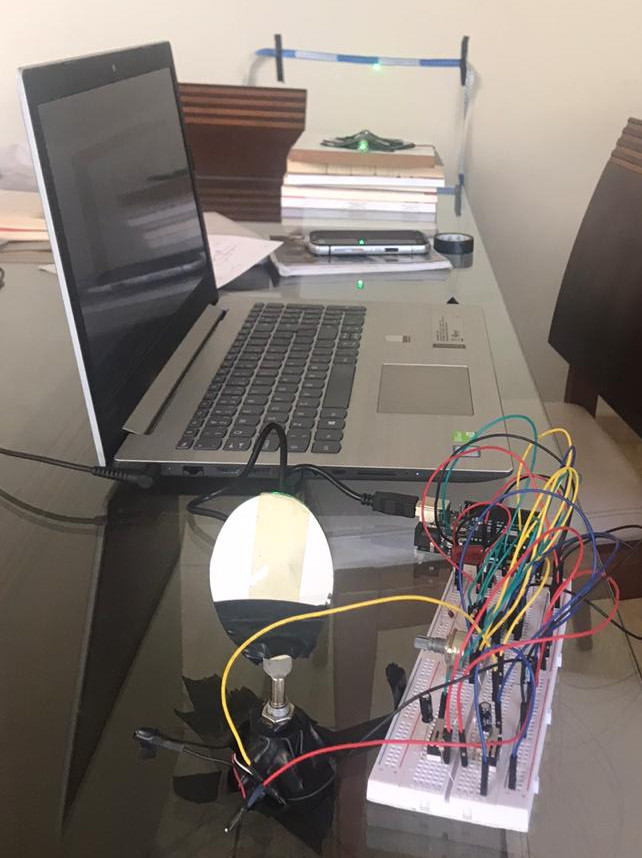
\includegraphics[width=0.5\columnwidth]{images/resultados/resolution.jpg} 
    \par\end{centering}

    \label{fig:result-resolution}
\end{figure}

O espelho atrelado ao potenciômetro foi então rotacionado manualmente até
que fosse vista uma mudança na leitura pelo Arduino. A distância percorrida
pelo \textit{laser} foi então medida com o auxílio de uma fita métrica, com
precisão milimétrica. Devido ao diâmetro observado do ponto de luz refletido 
sobre a parede, assumiu-se para o valor de $d$ uma incerteza associada de $\pm 10$mm.
Para a distância $D$, devido às limitações do ambiente de teste, e do instrumento de 
medição, uma trena com precisão milimétrica, adotou-se também uma incerteza de $10$mm.

A distância percorrida para uma variação angular mínima detectável pelo sensor 
foi de $32\pm 10$mm, com uma distância entre o sensor e a parede, de $2150\pm 10$mm. 
Com estes valores de $d$ e $D$, verifica-se que a angulação 
capaz de ser detectada pelo sensor é igual a $0,\!43\pm 0,\!14$\textdegree, segundo a 
equação \ref{eq:teste-pot}.

Embora o ambiente e os equipamentos de medição utilizados não fossem os mais adequados
para medições precisas, o teste demonstrou uma resolução próxima 
ao indicado no \textit{datasheet} do potenciômetro, disposto no anexo \ref{anexo-datasheets}, 
capaz de fornecer boas informações sobre o posicionamento das juntas.

\section{Circuitos de sensoriamento}

Foi preparado um protótipo da placa de sensoriamento, com dispositivos o mais próximo possível 
dos dispositivos reais projetados. O protótipo montado simulava o funcionamento de uma 
placa, contando com dois sensores do tipo fim-de-curso e uma conexão para um potênciometro.
Os dados dos sensores foram conectados a um CI amplificador que contava com 4 amplificadores
operacionais no mesmo dispositivo, o LM324. Os ganhos dos fim-de-curso foram configurados como 
unitários, de acordo com o esquemático da figura \ref{fig:Esquematico-sensor-switch}, já o ganho
do potenciômetro foi configurado como ajustável a partir de outro potenciômetro, este comum e de
volta única.

As conexões foram feitas completamente através de \textit{jumpers}, assim como pode ser visto na
figura \ref{fig:proto-sensor}.

\begin{figure}[h]
    \caption{Circuito de prototipagem do sensoriamento.}

    \begin{centering}
        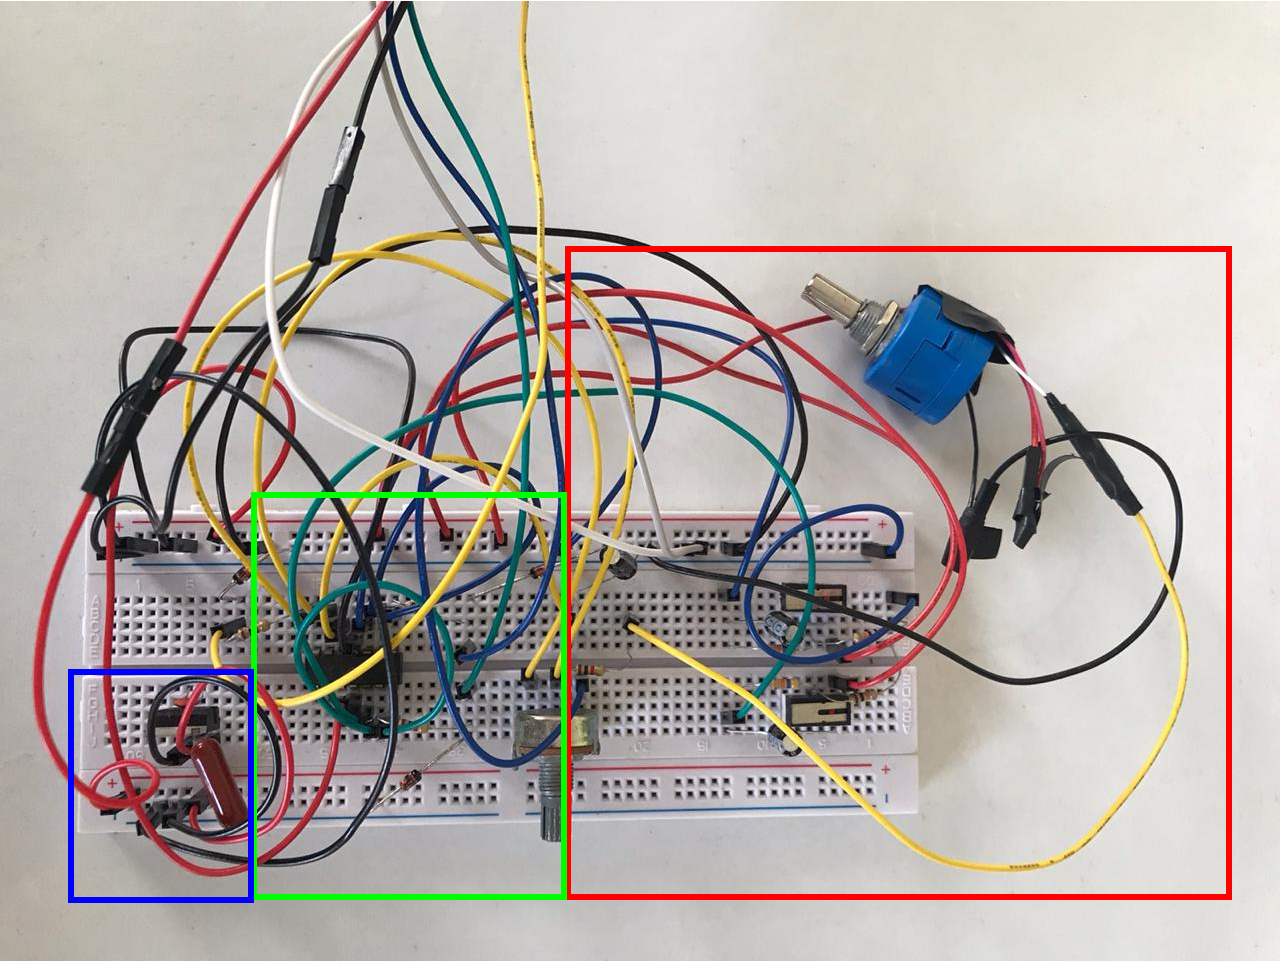
\includegraphics[width=0.75\columnwidth]{images/resultados/proto-sensor.jpeg} 
    \par\end{centering}

    \label{fig:proto-sensor}
\end{figure}

Na figura \ref{fig:proto-sensor} pode ser vista uma divisão espacial dos dispositivos
na placa de prototipagem de acordo com a sua funcionalidade. A área marcada pela
borda na cor vermelha indica os dispositivos sensores e os filtros iniciais de tratamento.
A área verde delimita principalmente a parte dos circuitos ligada à amplificação e à
preparação dos sinais para envio. Por fim, a área azul indica o circuito de alimentação,
com capacitores e regulador de tensão. Os 7 \textit{jumpers} que são vistos saindo da
placa são os que transmitem de fato os sinais para a placa central.

Para os testes e validação destes circuitos, os dados de saída foram conectados
diretamente à placa Arduino. Utilizando programas preparados especificamente para
este teste, foram verificados os valores dos sensores fim-de-curso antes e durante
sua ativação, garantindo que o valor correto seria repassado à etapa posterior
de tratamento. O valor do potenciômetro foi transformado em ângulo através de um
mapeamento linear. 

Foi verificado que para posições do eixo do potenciômetro próximo ao início, 
ocorriam variações indesejadas no valor de leitura, fruto das limitações do sensor.
Para contornar este problema foi definido que o valor mínimo para o qual estas 
variações não ocorrem seria posicionado como valor 0 da junta, limitando o movimento
do atuador para após esta posição por meio do uso dos sensores fim-de-curso. Esta posição
deve ser então definida com base em testes no ambiente real de aplicação do sensor, bem como
realizado no ambiente de testes.

Os circuitos se comportaram como esperado quando alimentados através de uma fonte de 
12V, com a tensão regulada através do circuito montado.

\section{Matriz Jacobiana inversa}
\label{sec:resultados-rotina}

Para validar a sub-rotina que implementa a transformação de velocidades do efetuador final
em velocidades das juntas, foi criado um \textit{script}, assim como já explicado na seção
\ref{sec:analise-cinematica}. A figura \ref{fig:test-vel} ilustra o funcionamento deste teste.

\begin{figure}[ht]
    \caption{Fluxograma programa de validação da jacobiana inversa.}

    \begin{centering}
        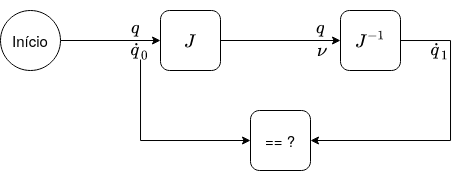
\includegraphics[width=0.6\columnwidth]{images/resultados/Test-vel.png} 
    \par\end{centering}

    \label{fig:test-vel}
\end{figure}

Os valores das posições e velocidades das juntas, $q$ e $\dot{q}$, são definidos no início do programa
e utilizados para calcular a velocidade do efetuador final, tomando-se como caminho de execução uma 
cinemática direta do manipulador. O vetor de velocidades obtido, $\boldsymbol{\nu}$, é então repassado à função
que implementa a inversa da matriz, juntamente com o vetor original de posições, para se obter um 
novo vetor de velocidade das juntas $\dot{\textbf{q}}_1$, a ser comparado com o vetor original de velocidades $\dot{\textbf{q}}_0$.

Foi verificado que para determinados valores das juntas o resultado final obtido era diferente do resultado
inicial configurado. Uma dessas configurações, e o seu valor final obtido, pode ser visto na tabela 
\ref{tab:res-jacobiana}.

\begin{table}[ht]
    \begin{centering}    
    
    \caption{Exemplo de resultado para conversão de velocidade.}
    
    \begin{tabular}{|c|c|c|c|}
        \hline
        $\textbf{q}$ & $\dot{\textbf{q}}_0$ & $\boldsymbol{\nu}$ = $\textbf{J}(\textbf{q}).\dot{\textbf{q}}_0$ & $\dot{\textbf{q}}_1$ = $\textbf{J}^{-1}(\textbf{q}).\boldsymbol{\nu}$ \tabularnewline
        \hline
        \hline
        $\pi/2$ & 0,21 & -0,08 & 0,21  \tabularnewline
        \hline
        $0$ & 0,14 & -0,55 & 0,11 \tabularnewline
        \hline
        $\pi/2$ & 0,85 & 0,04 & -0,11 \tabularnewline
        \hline
        $0$ & 0,01 & 0,88 & 0,88 \tabularnewline
        \hline
        $-\pi/2$ & 0,05 & -0,92 & 0,05  \tabularnewline
        \hline
        $0$ & 0,12 & 0,21 & 0,00 \tabularnewline
        \hline
    \end{tabular}

\label{tab:res-jacobiana}
    
\par\end{centering}
\end{table}

Foi constatado que estas discrepâncias eram resultado de um fator já esperado no uso
da matriz jacobiana inversa, os pontos de singularidade. Com o valor da junta 5 na tabela
\ref{tab:res-jacobiana}, o determinante da equação \ref{eq:det} seria igual a 0, o que 
acarretaria em uma matriz inversa com termos tendendo a $\pm\infty$, ou indeterminações.
Pelo método em que o cálculo da matriz foi organizado, cancelando termos comuns aos cofatores com termos
no determinante, foi possível arranjar alguns termos de 
modo que estas singularidades matemáticas não afetassem todas as juntas, o que é indicado pelo
fato que os resultados das juntas 1 e 5 apresentaram valores iguais aos originais.
Para demais valores de ângulos, que não resultam em singularidades, os valores obtidos após
a multiplicação por $\textbf{J}^{-1}$ foram iguais ao valores iniciais. Uma análise da equação
\ref{eq:det} fornece os pontos de singularidade do sistema, sendo estes pontos indicados pelos 
valores dos ângulos das juntas que fazem com que o determinante da matriz jacobiana seja nulo, a exemplo de algum
dos fatores $c\theta'_5$ ou $s\theta_3$ igual a 0, que forneceria o valor 0 para o determinante. 

A tentativa de otimizar os cálculos da matriz inversa, evitando o processamento gerado
por um código com diversos laços de repetição, resultou em uma função linear com 126
multiplicacões, 51 somas e 27 variáveis auxiliares. Frente a um código simples que calcularia
a inversa em $6^3$ iterações, o resultado obtido se mostrou satisfatório, mesmo quando aplicado
em um sistema embarcado, fornecendo resultados corretos em um bom tempo.

\section{Circuito central}

Em relação ao circuito central, por este ser composto de uma quantidade grande de 
dispositivos, foi idealizado um protótipo que agrupa as funções básicas de leitura
e tratamento dos sinais de uma única placa de sensoriamento e de acionamento de um
único motor de passo e um motor DC. o sistema completo pode ser visto na figura
\ref{fig:proto-main}.

\begin{figure}[ht]
    \caption{Circuito de prototipagem da placa central.}

    \begin{centering}
        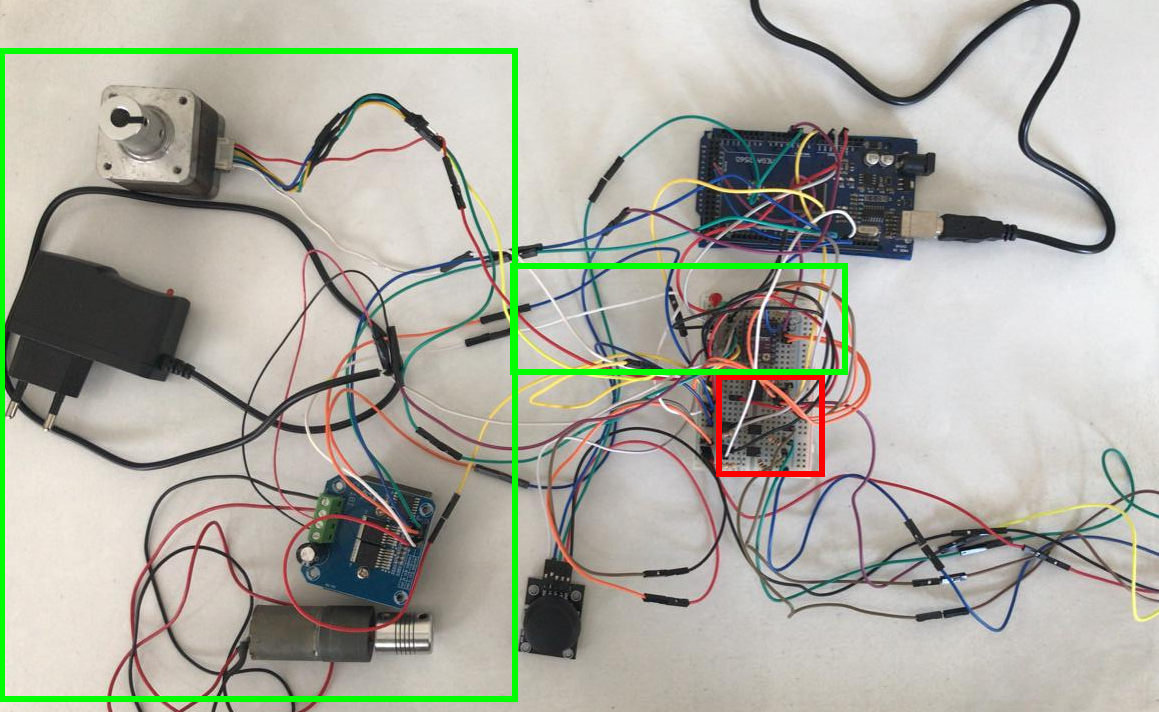
\includegraphics[width=1\columnwidth]{images/resultados/proto-main.jpeg} 
    \par\end{centering}

    \label{fig:proto-main}
\end{figure}

Nas áres indicadas pela cor verde, na figura \ref{fig:proto-main}, são vistos os 
dispositivos de acionamento e seus respectivos atuadores, bem como a fonte de 
alimentação utilizada nos testes para a potência destes.
A área em vermelho indica os dispositivos que realizam o tratamento dos sinais 
provindos da outra placa de prototipagem, como optoacopladores e amplificador operacional.
Na figura, podem ser vistos também o \textit{joystick} KY-023 utilizado e um Arduino Mega,
utilizados para interfaceamento com o usuário e processamento geral dos dados, respectivamente.

Nota-se que os atuadores empregados não são de fato iguais aos atuadores escolhidos para o 
sistema. Para os testes e prototipagem preferiu-se utilizar dispositivos genéricos, a fim 
de verificar a funcionalidade do circuito independente do modelo de atuador utilizado.

Foram realizados testes tanto para a simulação do sistema quanto para dados reais resultantes
da ativação dos atuadores, verificando e validando a comunicação entre as placas e os diversos circuitos
que compõem o sistema. Como não havia atuadores de teste suficientes para simular completamente
o circuito, foram realizadas combinações entre leitura real e simulação das juntas.

\section{Sistema de Comando}

\subsection{Tempo de execução do laço de repetição}

Foi verificado o tempo de execução para cada iteração do laço de repetição principal do
programa de comando, com as funções indicadas no fluxograma \ref{fig:fluxograma}.
Os tempos de execução observados ficaram entre 4 e 5ms, com a inclusão da rotina 
de envio dos dados ao computador, um tempo máximo de 7ms foi observado.

Vale a pena ressaltar que os tempos de execução não estarão sempre entre os valores
observados, sendo possível que alguma iteração do laço apresente maior tempo de 
duração, a depender de interrupções e outros fatores relativos ao sistema. No entanto,
os valores médios observados demonstraram uma boa resposta geral do sistema, com bom
tempo de resposta aos comandos humanos.

\subsection{Simulação}

Para simulação, definiu-se a diretiva ``\textit{SIMULATION}'' como 1 e então o sistema
foi energizado, para dar início ao seu funcionamento. Ao se iniciar a interface
em \textit{python} que se comunica com o circuito, é montada uma representação do 
manipulador utilizando os dados recebidos. A posição inicial foi definida para a simulação
como valores zero para as juntas com motores DC e os valores pós-calibração para as juntas 
com motores de passo. A figura \ref{fig:pos-inicial} ilustra o modelo gerado pelo simulador
assim que a aplicação é iniciada, com os eixos $\hat{X}$, $\hat{Y}$ e $\hat{Z}$ para cada junta.

\begin{figure}[h]
    \caption{Ambiente de simulação com posição inicial.}

    \begin{centering}
        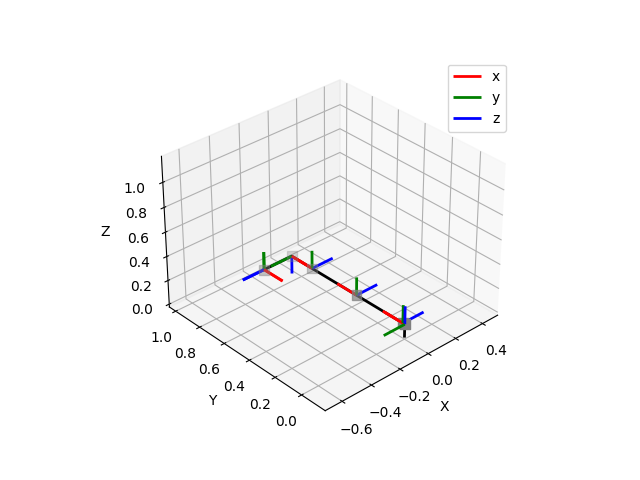
\includegraphics[width=0.8\columnwidth]{images/resultados/pos_inicial.png} 
    \par\end{centering}

    \label{fig:pos-inicial}
\end{figure}

Foi realizada uma tentativa de transportar o braço para a sua configuração zero, 
ou seja, com $\theta_i=0$ para $i$ de 1 a 6, para verificar a controlabilidade do sistema. 
O resultado obtido pode ser visto na figura \ref{fig:pos-zero}.

\begin{figure}[h]
    \caption{Ambiente de simulação com posição zero.}

    \begin{centering}
        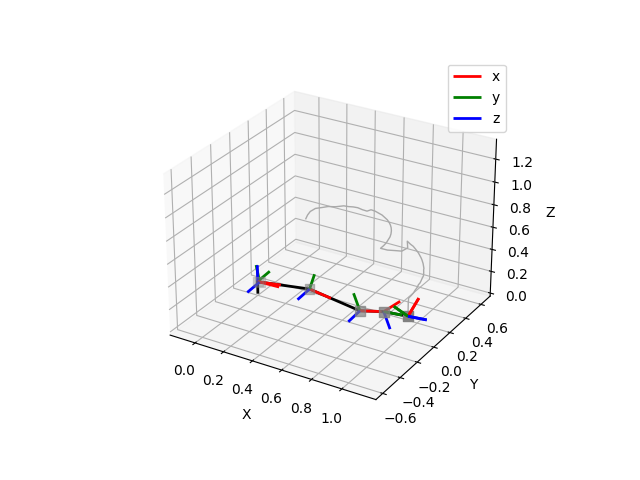
\includegraphics[width=0.8\columnwidth]{images/resultados/pos_zero.png} 
    \par\end{centering}

    \label{fig:pos-zero}
\end{figure}

Esta movimentação poderia ser realizada de vários modos, optou-se por agir inicialmente sobre a 
velocidade angular do eixo $\hat{Z}$ da junta 5 para deixar o último elo alinhado com o eixo $x$, utilizando o plano $R1$, e em 
seguida rotacionar o braço em torno da base utilizando o plano $XY$ e impondo uma velocidade
diagonal ao efetuador final ($v_x$ = $v_y$) através do joystick. 
Como o plano inicial definido no programa é o plano de translação $XY$,
foi necessário pressionar o botão do \textit{joystick} 2 vezes, alternando para o eixo $R1$ e depois mais
2 vezes, para retornar ao eixo $XY$. Ao final foi necessário modificar o plano de ação para o $XZ$, 
a fim de realizar um ajuste mais fino sobre a altura da posição desejada.

Nota-se na figura \ref{fig:pos-zero} uma indicação do trajeto percorrido pelo ponto final do 
manipulador. Esta trajetória é gerada com base nas velocidades impostas sobre o efetuador
final do sistema, que são transformadas em velocidades simultâneas das juntas, para movimentar corretamente
todo o manipulador, de acordo com o desejo de movimento do usuário.

O processo foi repetido tentando atingir outras posições e orientações para o robô, algumas dessas
configurações estão dispostas nas imagens \ref{fig:pos-varias}(a)-(e).

\begin{figure}[h!]
    \begin{centering}

    \begin{floatrow}

        \subfloat[Braço posicionado no alto.]{
            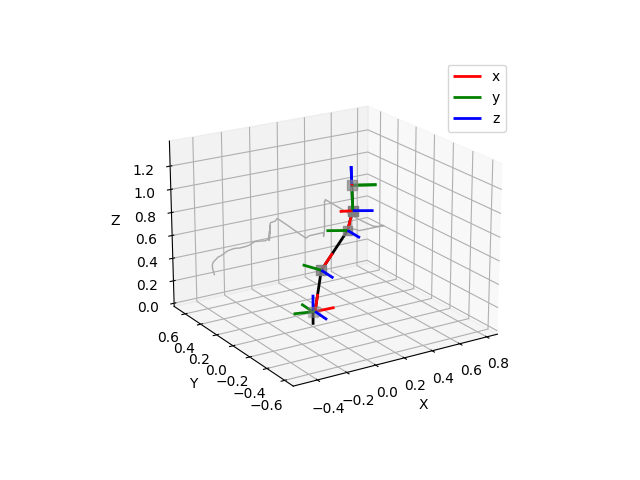
\includegraphics[width=0.5\columnwidth]{images/resultados/pos_z.png}
        }

        \subfloat[Braço na posição de alimentação.]{
            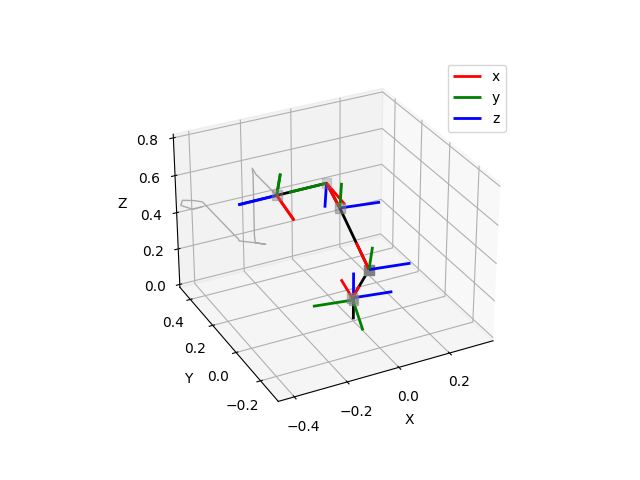
\includegraphics[width=0.5\columnwidth]{images/resultados/pos_alimento.png}
        }

    \end{floatrow}

    \begin{floatrow}

        \subfloat[Braço para pegar objetos na frente do usuário - alto.]{
            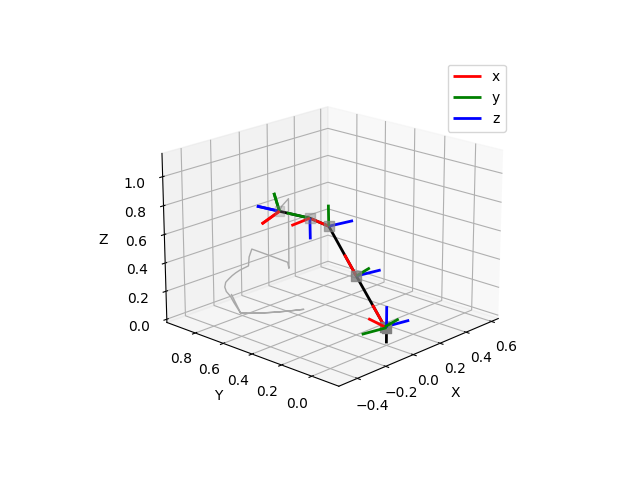
\includegraphics[width=0.5\columnwidth]{images/resultados/pos_pegar1.png}
        }
    
        \subfloat[Braço para pegar objetos na frente do usuário - baixo.]{
            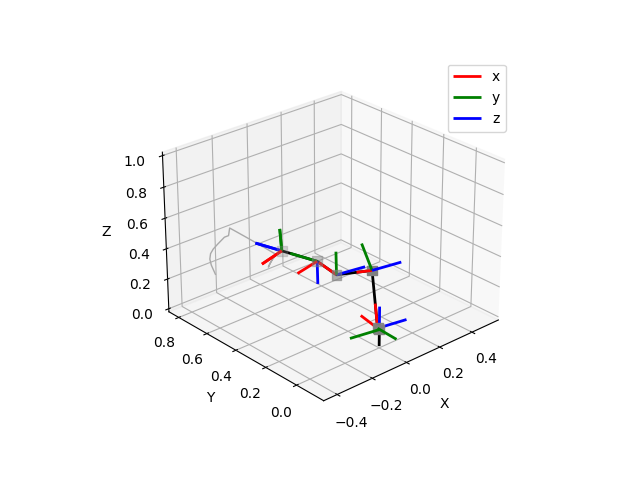
\includegraphics[width=0.5\columnwidth]{images/resultados/pos_pegar2.png}
        }
    
    \end{floatrow}

    \subfloat[Braço na posição de singularidade.]{
        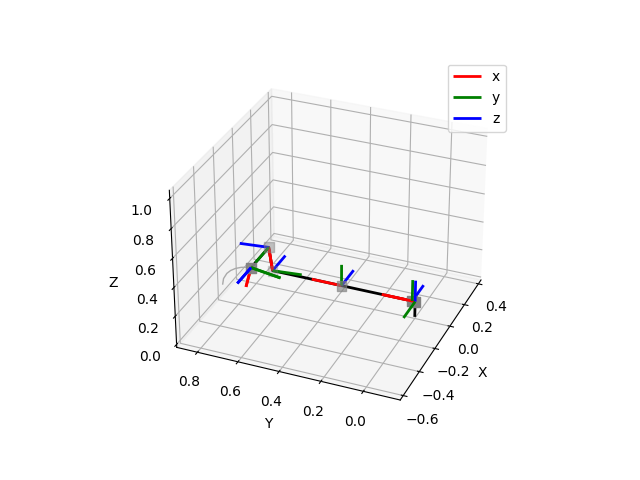
\includegraphics[width=0.5\columnwidth]{images/resultados/pos_singularidade.png}
    }

\caption{Diversas configurações do manipulador simulado.}
\label{fig:pos-varias}

\par\end{centering}
\end{figure}

Alguns pontos de interesse foram os pontos de singularidade do robô. Nestes pontos, é comum
que haja a perda de um dos graus de liberdade do manipulador. A figura \ref{fig:pos-varias}(e) 
ilustra este fato, onde o ângulo de $\theta_5 = -\pi/2$ gera uma singularidade apontada previamente.
Neste ponto específico, os eixos $\hat{Z}_4$ e $\hat{Z}_6$ se tornam coplanares, portanto uma 
rotação em torno de $\hat{Y}_5$ acaba gerando uma indefinição sobre qual dos ângulos deve ser
atuado. Nota-se pelo resultado obtido que a geração de velocidades pela matriz jacobiana favorece a atuação
na junta 4.

\subsection{Atuadores reais}

Para os testes com atuadores reais, foram preparados um motor de passo e um motor DC. Cada
sistema de motor foi marcado de certo modo a permitir a identificação de sua rotação efetiva. 

Inicialmente, ao invés de utilizar dados de simulação, o programa foi modificado para realizar 
a leitura real da junta 1, e a esta junta foi atrelado logicamente um motor de passo, via definição em código. 
Foi realizado então o mesmo procedimento utilizado para geração dos resultados da figura 
\ref{fig:pos-zero}, observando a rotação do motor de passo. Os resultados reais obtidos 
com o atuador para esta junta estão organizados na figura \ref{fig:result-stepper}.
Para indicar que o ponto de calibração foi atingido, foi utilizado um dos sensores da placa 
de prototipagem de sensoriamento.

\begin{figure}[h!]
    \begin{centering}

    \begin{floatrow}

        \subfloat[Motor de passo na posição pós-calibração.]{
            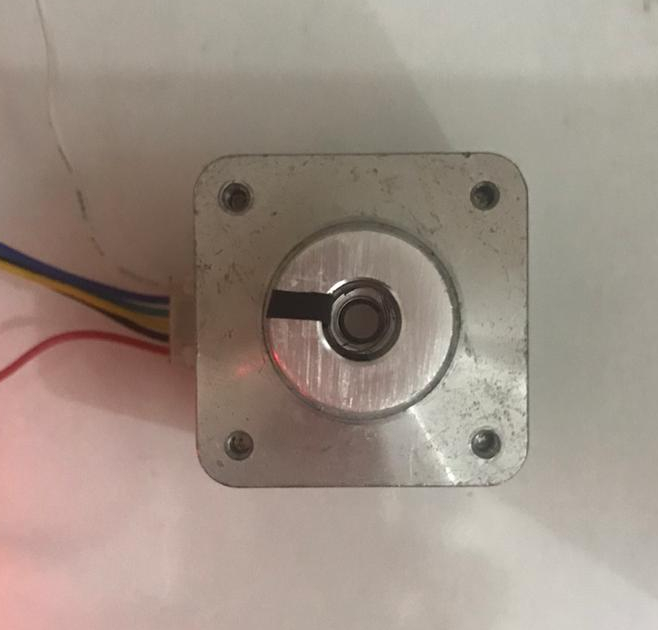
\includegraphics[width=0.3\columnwidth]{images/resultados/stepper1.jpeg}
        }

        \subfloat[Motor de passo após atingir posição desejada.]{
            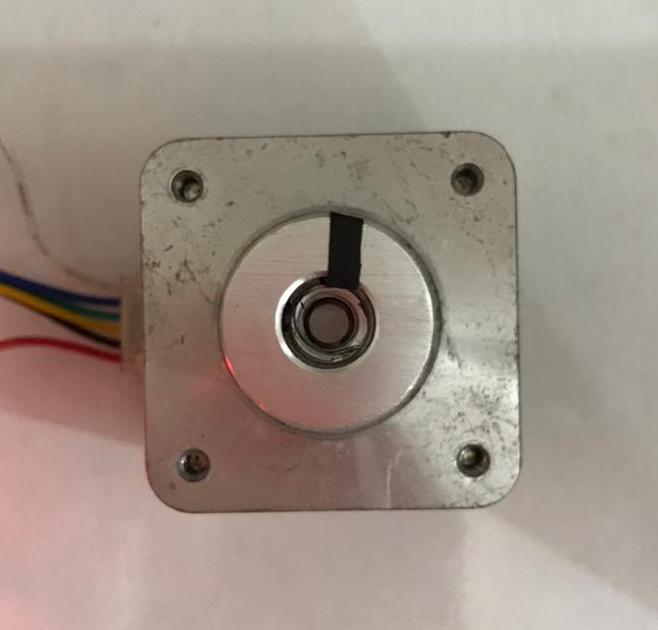
\includegraphics[width=0.3\columnwidth]{images/resultados/stepper2.jpeg}
        }

    \end{floatrow}

    \subfloat[Posição final obtida.]{
        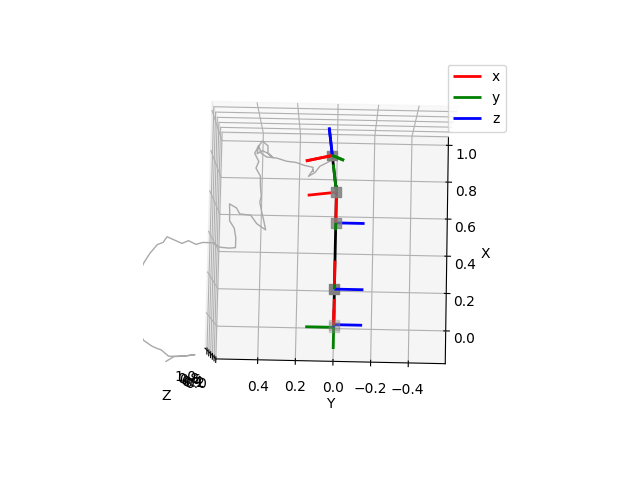
\includegraphics[width=0.8\columnwidth]{images/resultados/pos_stepperfinal.png}
    }

\caption{Resultado com atuação de motor de passo.}
\label{fig:result-stepper}

\par\end{centering}
\end{figure}

As figuras \ref{fig:result-stepper}(a) e \ref{fig:result-stepper}(b) indicam que a rotação
real obtida com os motores de passo aproximou-se da rotação de 90\textdegree\, desejada para
a junta da base. 

Experimentos semelhantes foram realizados para as juntas 5 e 6, que também utilizam motores 
de passo. Os resultados reais de posicionamento foram comparados visualmente com os resultados
obtidos com a animação no ambiente de simulação. Em especial, foram utilizados os planos de ação
$R1$ e $R2$, que permitem atuar diretamente sobre os motores destas juntas, por estarem
relacionados com o movimento de \textit{roll} e \textit{yaw} do pulso.
Visualmente, o atuador de teste acompanhou de fato o movimento imposto para o manipulador através das 
velocidades definidas no \textit{joystick}.

Para as outras juntas, que utilizam motores DC, foi preparado um ambiente de testes que consistia
no acoplamento direto entre o eixo de saída de um motor DC de teste e um potenciômetro, assim
como demonstra a figura \ref{fig:teste-dc}. Ambos motor e sensor foram fixados de modo a fornecer
uma resistência mecânica, através do uso de fita adesiva, contra rotação que não fosse do próprio eixo.

\begin{figure}[h!]
    \begin{centering}

    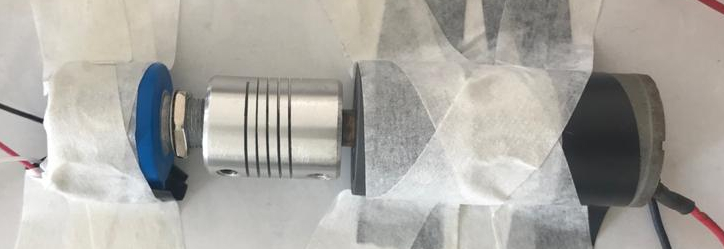
\includegraphics[width=0.8\columnwidth]{images/resultados/teste-dc.jpeg}

\caption{Montagem de teste para motores DC.}
\label{fig:teste-dc}

\par\end{centering}
\end{figure}

A rotina realizada foi semelhante àquela dos motores de passo: Foram conferidas as posições iniciais
indicadas na simulação e no sistema real, e estas foram posteriormente comparadas após uma
sequência de comandos de velocidades informadas via \textit{joystick}. O motor DC foi atribuído à junta 2,
o ombro do sistema. 
A figura \ref{fig:result-dc} agrupa as posições observadas, tanto no ambiente de simulação quanto no ambiente 
real. O ganho do sensor foi ajustado via potenciômetro na placa de prototipagem do sensoriamente para
aproximadamente 2, isto é visível pela figura \ref{fig:result-dc}, onde a simulação indica uma variação
angular próxima a 45\textdegree, mas o sistema real aponta algo mais próximo de 90\textdegree.

\begin{figure}[h!]
    \begin{centering}

    \begin{floatrow}

        \subfloat[Motor DC na posição inicial.]{
            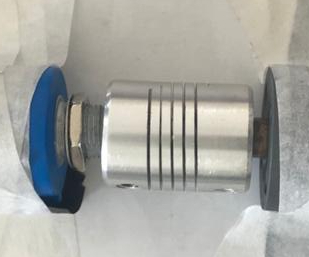
\includegraphics[width=0.4\columnwidth]{images/resultados/dc-real1.jpeg}
        }

        \subfloat[Motor DC na posição final.]{
            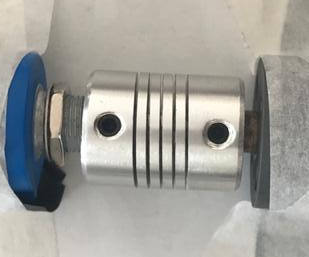
\includegraphics[width=0.4\columnwidth]{images/resultados/dc-real2.jpeg}
        }

    \end{floatrow}

    \begin{floatrow}

        \subfloat[Simulação com valor real de motor DC - inicial.]{
            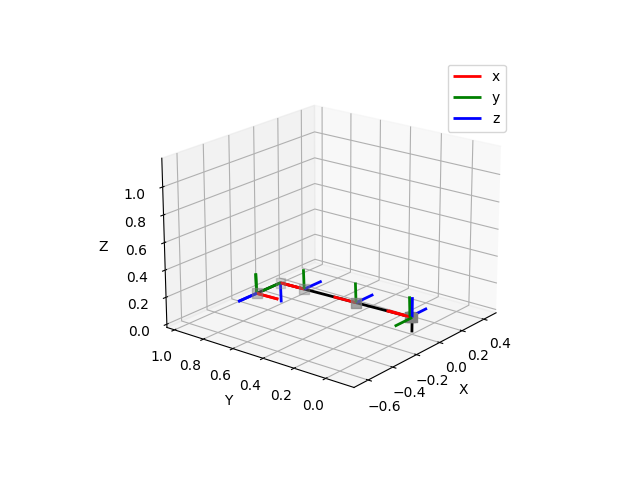
\includegraphics[width=0.5\columnwidth]{images/resultados/pos_dc_inicial.png}
        }

        \subfloat[Simulação com valor real de motor DC - final.]{
            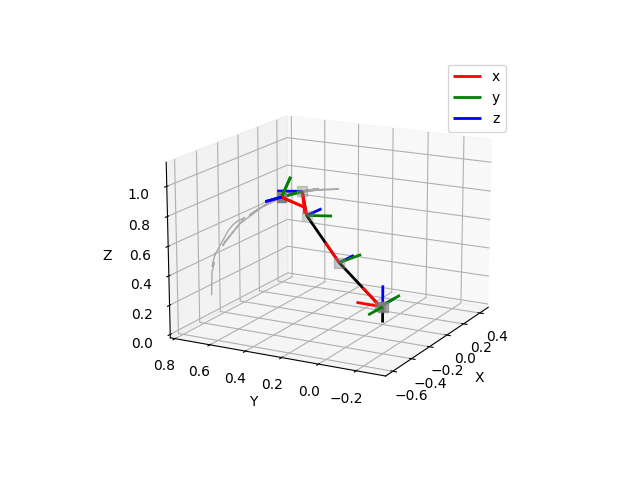
\includegraphics[width=0.5\columnwidth]{images/resultados/pos_dc_final.png}
        }

    \end{floatrow}

\caption{Resultado com atuação de motor de passo.}
\label{fig:result-dc}

\par\end{centering}
\end{figure}

As respostas para ambos os motores foram satisfatórias, observando-se que a variação angular real alcançada
por estes estava de acordo com o desejado pelo usuário para um posicionamento final do manipulador. 
Este fato indica a controlabilidade dos atuadores via \textit{input} do \textit{joystick} e a correta 
transmissão dos sinais de leitura. 
Os testes com os sensores potenciômetros de precisão demonstraram que a leitura de posição, 
e consequentemente a resposta de todo o sistema, é favorecida através do uso de toda ou grande
parte da área de trabalho do sensor, utilizando uma transmissão entre o eixo de saída e o eixo
do sensor. 

Os motores DC demonstraram ainda uma dificuldade de trabalho em baixas velocidades, resultando em
complexidades no ajuste fino para o posicionamento final. Acredita-se que este problema será mitigado
no sistema real, pelo uso das relações de transmissão, resultando em uma velocidade mínima menor do que 
a de saída do atuador.

Foi verificada por fim a resposta do sistema com os dados reais dos dois motores, DC e de passo, e complementando
o sistema com a simulação das outras 4 juntas. Uma das posições finais desejadas está disposta na figura 
\ref{fig:pos-dois}, simulando o desejado de obtenção de algum objeto à frente do usuário.

\begin{figure}[h!]
    \begin{centering}

    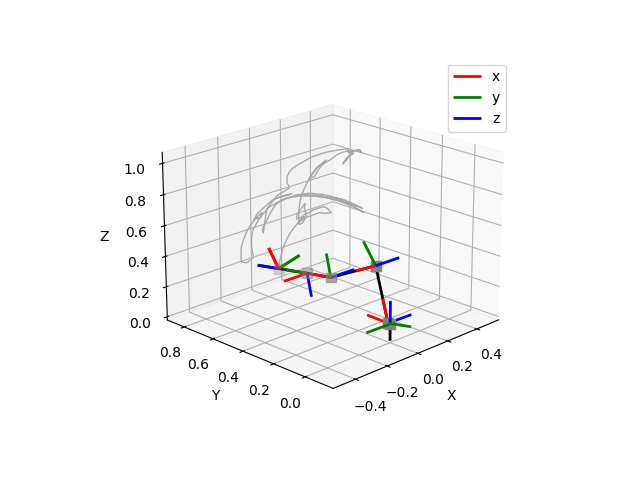
\includegraphics[width=0.8\columnwidth]{images/resultados/pos-dois.png}

\caption{Simulação com dados reais de 2 motores.}
\label{fig:pos-dois}

\par\end{centering}
\end{figure}

A operação do sistema indica o correto funcionamento tanto dos circuitos projetados para atuação e
sensoriamento do braço mecânico. Embora os resultados foram obtidos com protótipos, espera-se que 
os circuitos reais ofereçam resultados similares e/ou melhores, por contarem com dispositivos mais
adequados, seguindo as especificações do projeto.

\begin{comment}
Conclusões
\end{comment}
\chapter{Conclusões}

\label{CapConclusoes}

Foram demonstrados durante o trabalho uma análise do projeto que serviu como base para este e os projetos
de circuitos de atuação e sensoriamento para o manipulador robótico em questão. As diversas decisões de 
projeto foram orientadas pelo custo de manufatura e montagem dos dispositivos, segurança aos equipamentos e ao 
usuário e pela confiabilidade geral do circuito elétrico e sistema de comando, buscando desenvolver uma 
solução que se mostrasse capaz de ser uma interface entre o usuário e seu ambiente.

A análise do conjunto de atuadores pré-selecionado para o braço robótico e suas respectivas transmissões 
através de engrenagens se mostrou insuficiente para a movimentação correta do sistema. Foi necessário 
propor modificações em algumas juntas para que as necessidades de torque pudessem ser de fato atendidas.

Os circuitos projetados e escolhidos para o sistema demonstraram bons resultados no uso com sensores e atuadores reais. 
A escolha dos equipamentos levou em consideração um equilíbrio entre o custo e integridade 
dos sinais envolvidos, fornecendo dados de leitura corretos mesmo para um protótipo construído com dispositivos e 
condições não ideais, em ambiente de testes sem ferramental próprio para execução no manipulador real.

Em relação ao sistema de comando, foram criados módulos generalizados e intuitivos, para permitir reaproveitamento de código em 
outros projetos. A organização geral e uso de interrupções em \textit{software} permitiu uma resposta rápida do sistema a modificações
das variáveis lidas por sensores e uma simplicidade no fluxograma principal do código, resultando em um aproveitamento
das diversas funcionalidades oferecidas pelo controlador empregado. Esta decisão facilitou ainda a operação
dos atuadores em paralelo, essencial no acionamento de um manipulador robótico.

A técnica de obtenção das velocidades do robô através da matriz jacobiana inversa facilitou a atualização das
referências das velocidades dos motores com base nos dados do usuário. A otimização desta matriz 
em sua forma de função ofereceu resultados satisfatórios, permitindo a operação de inversão desta matriz
relativamente trabalhosa em um ambiente embarcado.

O ambiente de simulação criado inicialmente como um meio de contornar a ausência da estrutura física do
manipulador se mostrou como bom meio de visualizar e validar os equipamentos do mesmo. A comunicação
entre o sistema embarcado e um computador gera uma pequena sobrecarga sobre o Arduino, mas esta é compensada pela capacidade
de utilizar sistema computacional mais potente para realizar estudos avançados sobre a estrutura,
como através das equações de Newton-Euler, já implementadas no módulo de animação, para estimar os torques agindo nos
atuadores.

Todo o material desenvolvido durante este trabalho, inclusive aqueles utilizados na construção deste 
relatório, está agrupado em um repositório \textit{online}, para consultas e confirmação do que foi 
dito e afirmado neste documento. Uma descrição do repositório pode ser vista no apêndice \ref{Anexo-Repositorio}.

\section{Perspectivas Futuras}

% Cinemática inversa
A atuação do manipulador foi comandada completamente pelo uso da geração de velocidades através da matriz
jacobiana inversa. Para facilitar o uso pelo usuário, pensou-se na possibilidade de utilizar um meio de 
salvar posições de maior uso pelo usuário, como posições de alimentação e captura de objetos em determinada 
posição. Tendo em mente esta capacidade, foi realizada a cinemática inversa do manipulador, para direcionar
trabalhos futuros na inclusão desta funcionalidade ao manipulador. A cinemática inversa pode ser vista no apêndice
\ref{Anexo-CinInv}.

% Controle mais avançado
O formato em que o controle dos motores DC foi projetado levou em consideração a possibilidade de uso de técnicas 
de controle mais avançadas. A utilização de uma interrupção temporizada permite o emprego de sistemas de controle
digital com período de atualização bem definido. Para maior confiabilidade na atuação dos motores DC pode ser 
previsto o uso de um controlador adaptativo, resultando em um controlador geral, independente da influência dos 
parâmetros construtivos do motor empregado. Levando em conta a segurança do usuário, poderia ser proposto ainda 
para o sistema um método de implementação de um controle complacente, utilizando dados de torque nas juntas e no
efetuador final a fim de evitar forças desnecessárias na atuação do robô.

% Testes com diferentes efetuadores finais
Em seu estado atual, o manipulador não conta com um efetuador final bem definido, mas sim com um ponto 
de acoplamento. Seria interessante um estudo sobre a possibilidade de aplicação de diversas ferramentas 
pelo sistema. Para interação com esse efetuador, foi deixado no circuito da placa principal um conector
para ser empregado nesta comunicação, fornecendo um sinal com funcionalidade PWM, para uso com servo-motores 
ou qualquer outro atuador que possa se beneficiar deste tipo de sinal.

% Modificações na estrutura
Se mostrando como uma das principais dificuldades encontradas durante o projeto, a estrutura mecânica do 
manipulador poderia ser modificada para aproveitar ao máximo os diversos componentes empregados. A 
modificação das juntas para incluir caixas de redução harmônicas permitiria o uso de motores de baixo 
torque, garantindo uma melhor resposta do sistema, principalmente nas juntas 2, 3 e 4.

\begin{comment}
Bibliografia
\end{comment}

\renewcommand{\bibname}{REFERÊNCIAS BIBLIOGRÁFICAS}
\addcontentsline{toc}{chapter}{REFERÊNCIAS BIBLIOGRÁFICAS}

\bibliographystyle{abnt-num}
\bibliography{bibliography}

\begin{comment}
  Apêndice
\end{comment}

\begin{comment}
Anexos
\end{comment}

%\anexos
\makeatletter
% não retirar estes comandos
\renewcommand{\@makechapterhead}[1]{%
  {\parindent \z@ \raggedleft \setfontarial\bfseries
\LARGE \thechapter. \space\space
\uppercase{#1}\par
\vskip 40\p@
}
}
\makeatother

\begin{comment}
Anexo I: Descrição do repositório.   
\end{comment}

%
\chapter{Descrição do Repositório}

\label{Anexo-Repositorio}

O \textit{link} de acesso do repositório é ``https://github.com/rafael-at97/WMRA-UnB''. A 
oganização do mesmo, indicando principais arquivos e diretórios pode ser vista na figura
\ref{fig:repositorio}.

\begin{figure}[h]
    \caption{Organização do respositório.}    

    \begin{centering}
        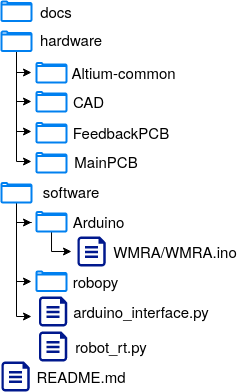
\includegraphics[width=0.3\columnwidth]{images/anexo/repositorio.png} 
    \par\end{centering}

    \label{fig:repositorio}
\end{figure}

Todos os arquivos necessários para a criação deste documento estão dentro da pasta `\textit{docs}',
os arquivos de texto estão no formato LATEX.

A pasta \textit{hardware} agrupa todos os arquivos relacionados a partes físicas do projeto,
como as bibliotecas desenvolvidas para representar circuitos eletro-eletrônicos criadas
durante o projeto dos circuitos, pasta `\textit{Altium-common}', documentos do projeto das 
placas em si, pastas `\textit{FeedbackPCB}' e `\textit{MainPCB}' e o modelo 3D do manipulador, na 
pasta `\textit{CAD}'.

Já o que foi desenvolvido em relação a partes lógicas do sistema estão dispostos dentro da pasta
`\textit{software}'. Na pasta `Arduino' encontram-se todas as bibliotecas desenvolvidas para o 
sistema embarcado e o código principal utilizado para o controle geral do sistema, denominado
por `WMRA/WMRA.ino'. A pasta `\textit{robopy}' faz alusão a outro repositório, também criado pelo
autor deste documento, que organiza as interpretações das funções da \textit{toolbox} de robótica
para MATLAB, mas em uma versão escrita em \textit{python}. O código `\textit{arduino\_interface.py}'
realiza a interface entre os dados vindos do arduino e o módulo de simulação. A criação da representação
do manipulador utilizando os módulos desenvolvidos está no arquivo `\textit{robot\_rt.py}', que tenta 
realizar a atualização do modelo em tempo real, ou \text{real-time}.

Por fim, há um arquivo `\textit{README.md}', que fornece informações básicas sobre o projeto.


%\refstepcounter{noAnexo}

\begin{comment}
  Anexo II: Catalógo de Equipamentos
\end{comment}

%\chapter{Fichas catalográficas}

\section{Mabuchi JC/LC-578VA}

\label{Mabuchi}

\begin{figure}[h]   
\begin{centering}
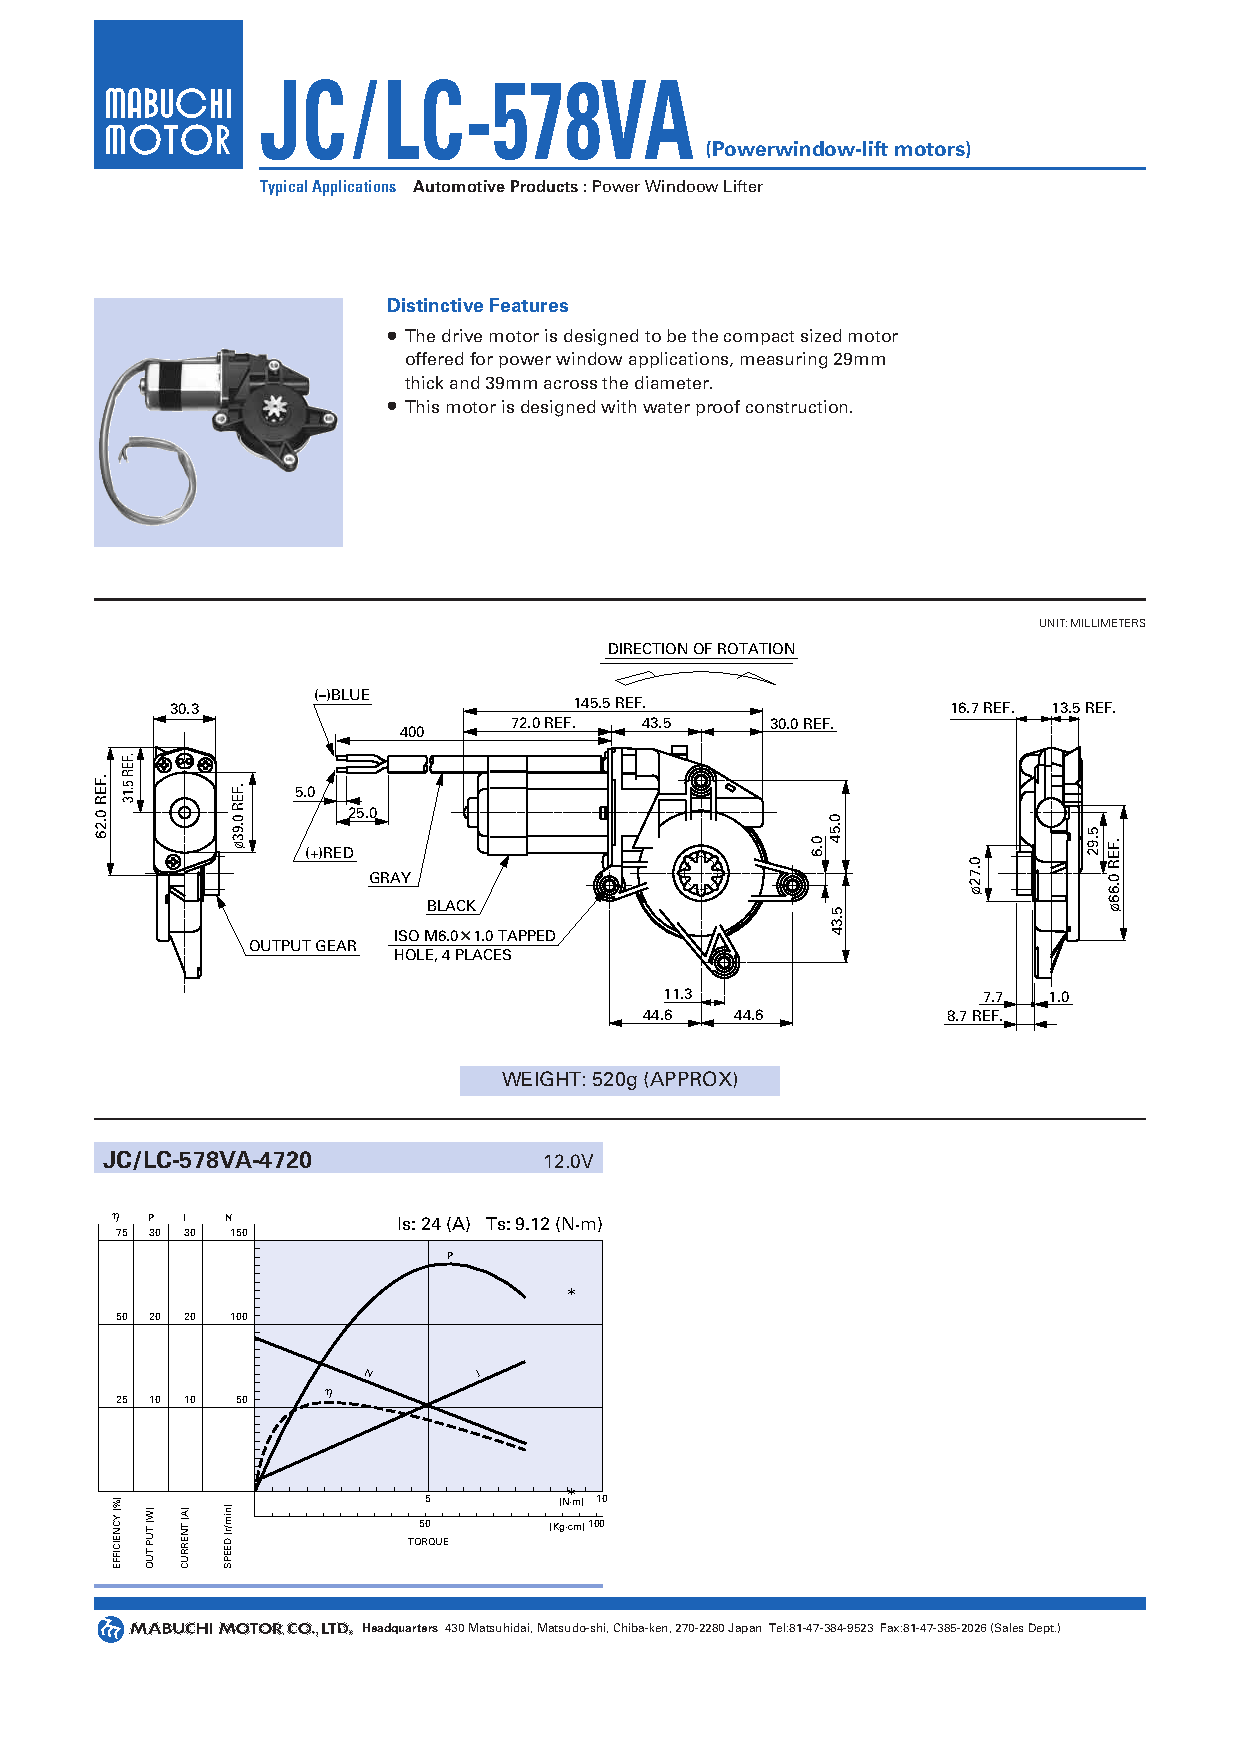
\includegraphics[width=0.8\columnwidth]{datasheets/mabuchi.pdf}
\par\end{centering}

\end{figure}

\section{HT23-397}

\label{HT23}

\begin{figure}[h]   
\begin{centering}
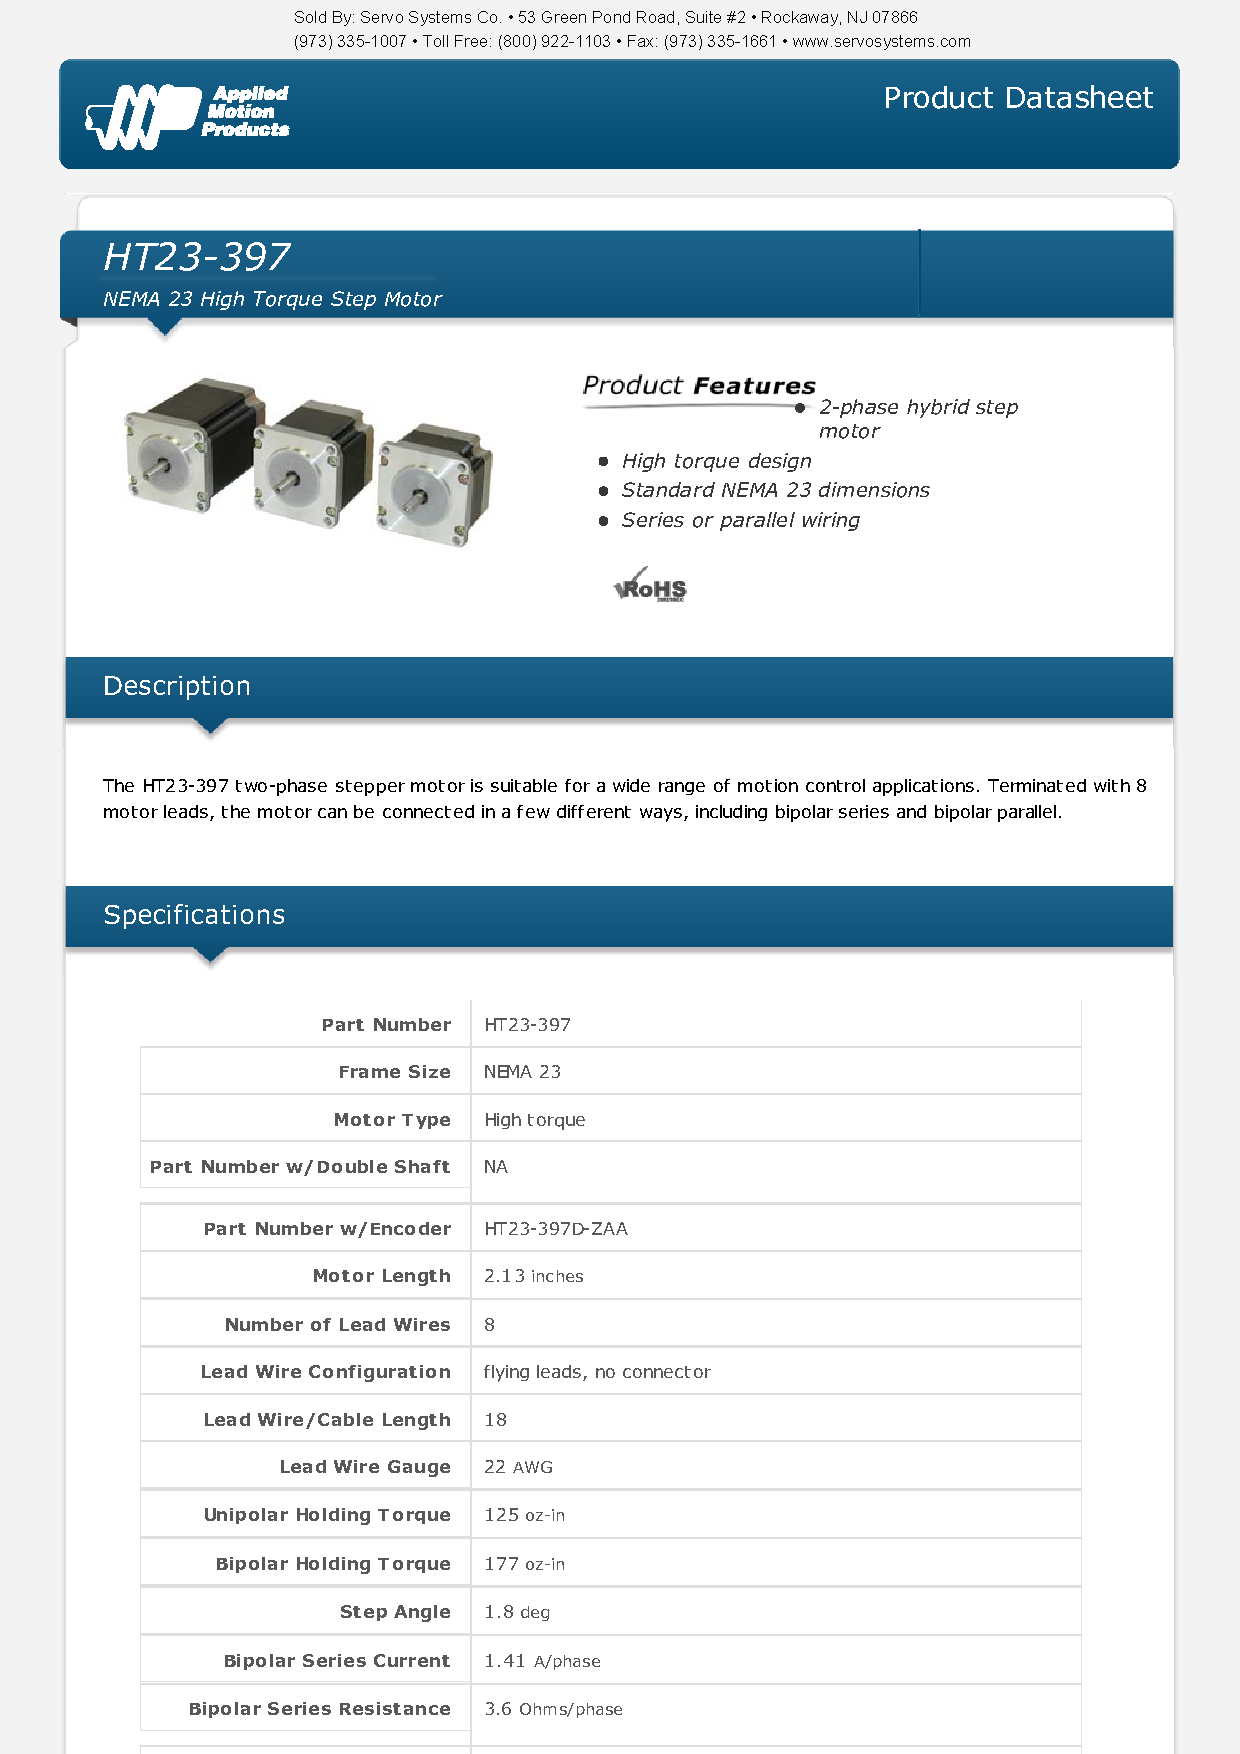
\includegraphics[width=0.81\columnwidth]{datasheets/ht23-397.pdf}
\par\end{centering}

\end{figure}
\newpage

\section{42HK \textit{Family Series}}

\label{42HK}

\begin{figure}[h]   
\begin{centering}
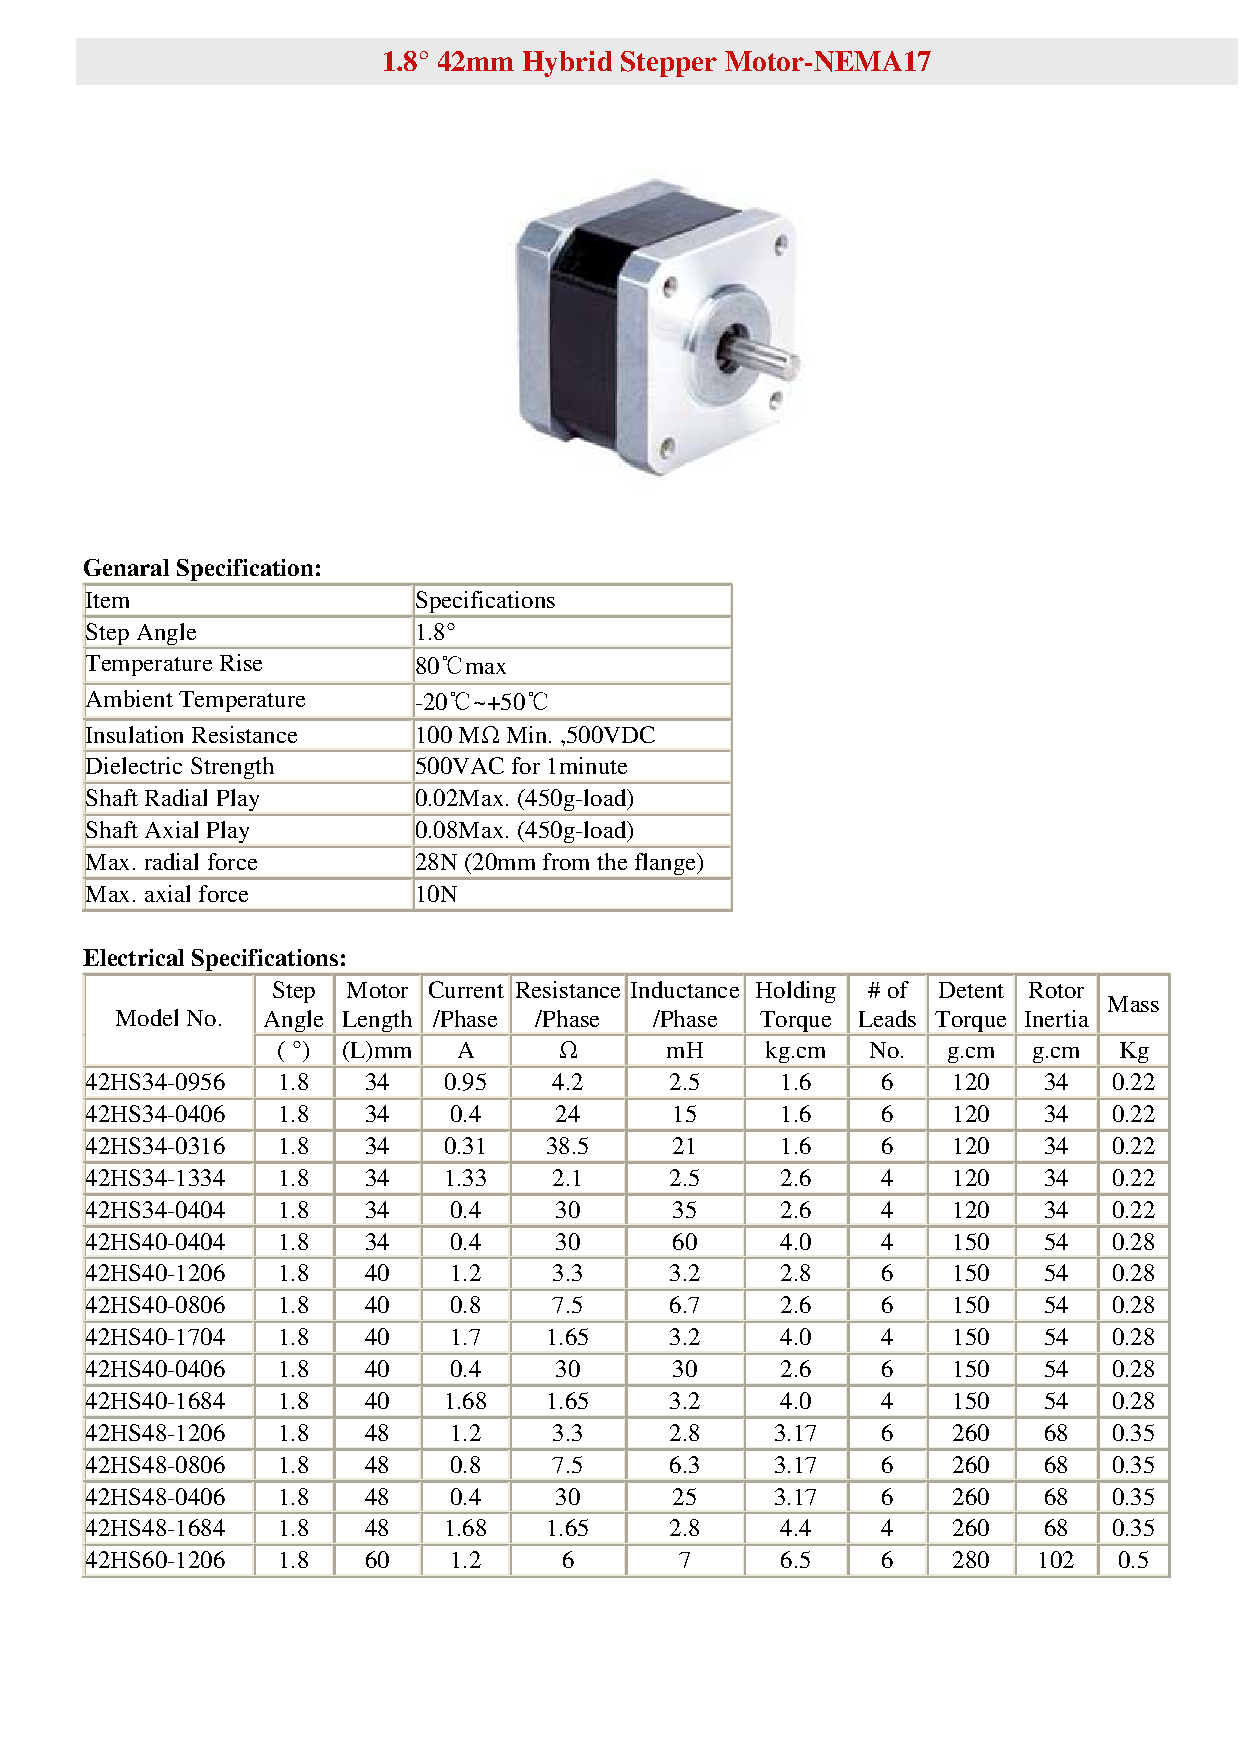
\includegraphics[width=0.81\columnwidth]{datasheets/jk42.pdf}
\par\end{centering}

\end{figure}
\newpage

\section{Bourns - 3590}

\label{BournsPot}

\begin{figure}[h]   
\begin{centering}
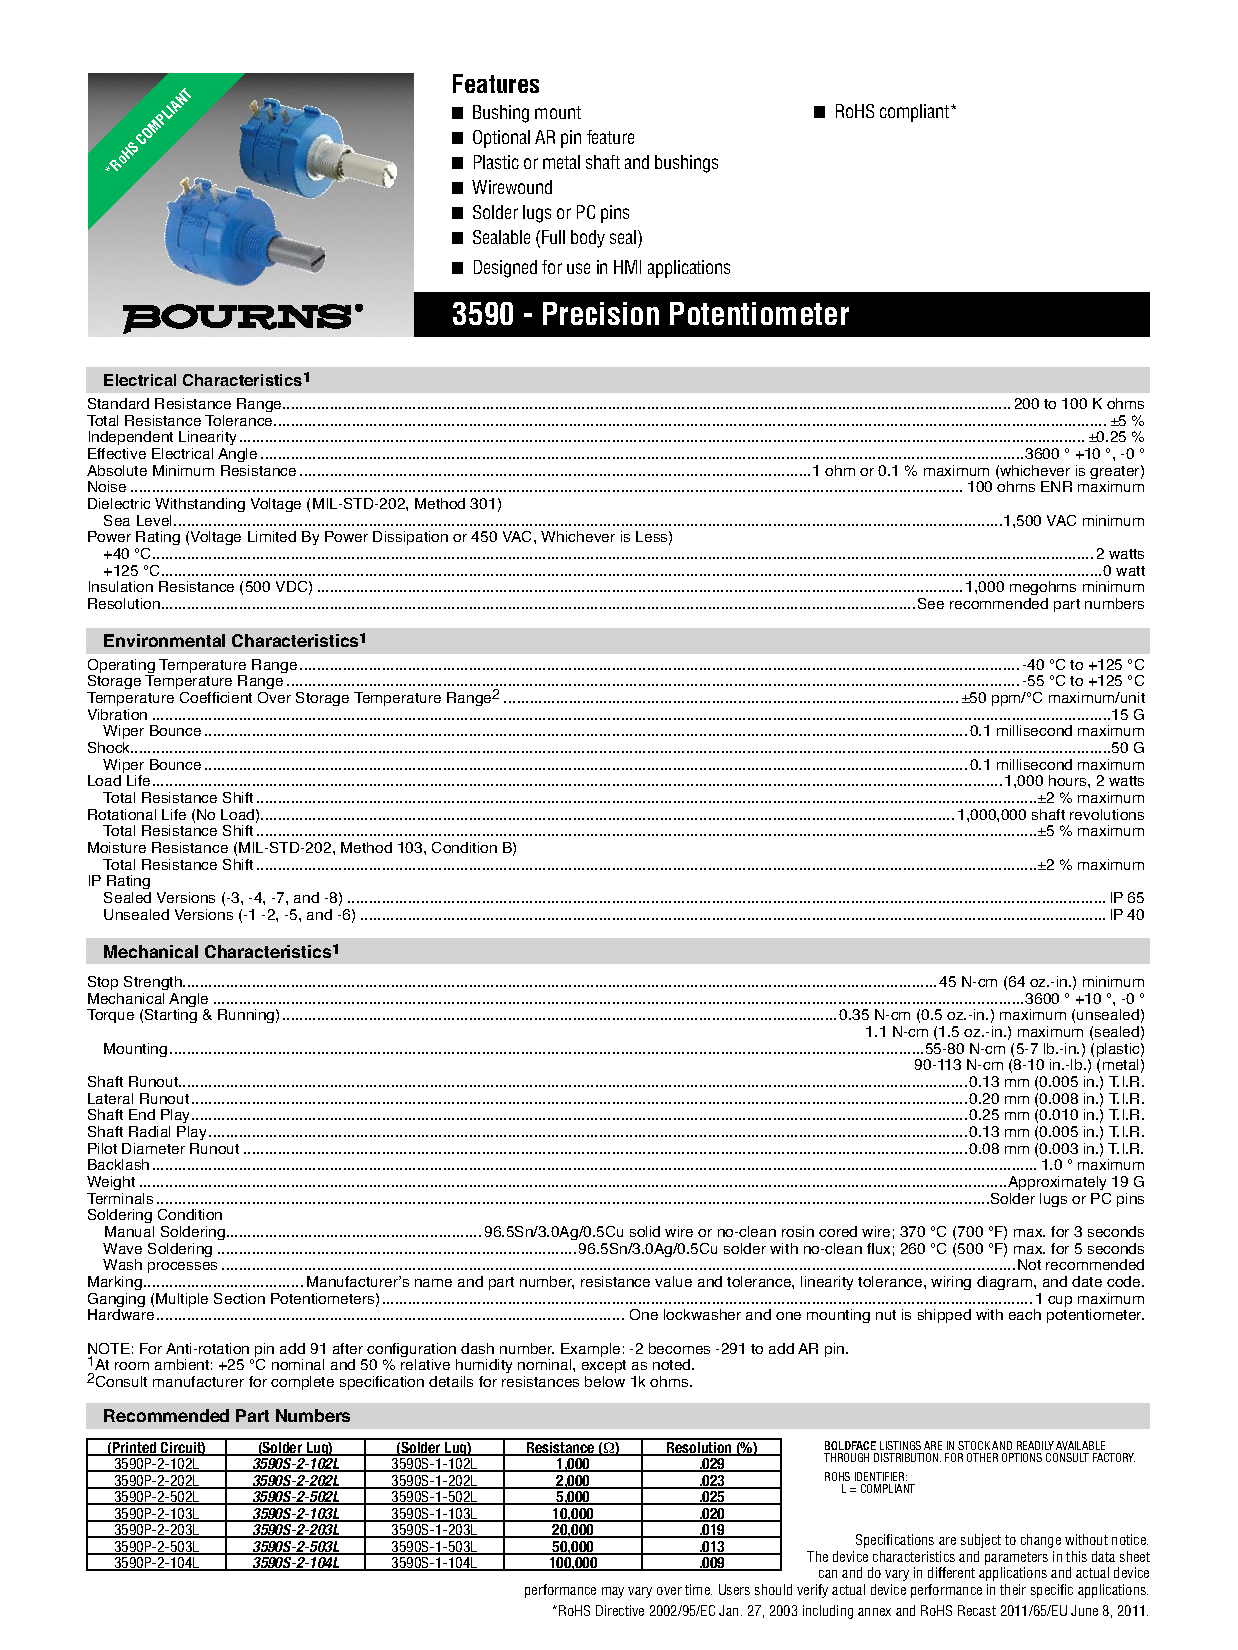
\includegraphics[width=0.85\columnwidth]{datasheets/bournspot.pdf}
\par\end{centering}

\end{figure}

%\refstepcounter{noAnexo}

\begin{comment}
Anexo III: Cinemática Inversa
\end{comment}

%\chapter{Cinemática Inversa para o Manipulador}
\label{Anexo-CinInv}

%\chapter{Matrizes auxiliares calculadas para a análise cinemática do manipulador}
%\label{AnexoCinematica}

\section{Transformações}
\label{AnexoJacobiana-Transformacoes}

Inicialmente, agrupando as duas últimas transformações.

\begin{equation}
    ^4_6T = ^4_5T*^5_6T =   \begin{bmatrix}
                                s\theta_5'c\theta_6 & -s\theta_5's\theta_6 & c\theta_5' & c\theta_5'd_6 + a_4 \\
                                s\theta_6 & c\theta_6 & 0 & 0 \\
                                -c\theta_5'c\theta_6 & c\theta_5's\theta_6 & s\theta_5' & s\theta_5'd_6 \\
                                0 & 0 & 0 & 1 \\
                            \end{bmatrix}
\end{equation}

Incluindo a transformação $^3_4T$:

\begin{equation}
    ^3_6T = ^3_4T*^4_6T =   \begin{bmatrix}
                                c\theta_4s\theta_5'c\theta_6 - s\theta_4s\theta_6 & -c\theta_4s\theta_5's\theta_6 - s\theta_4c\theta_6 & c\theta_4c\theta_5' & c\theta_4c\theta_5'd_6 + c\theta_4a_4 + a_3 \\
                                s\theta_4s\theta_5'c\theta_6 + c\theta_4s\theta_6 & -s\theta_4s\theta_5's\theta_6 + c\theta_4c\theta_6 & s\theta_4c\theta_5' & s\theta_4(c\theta_5'd_6 + a_4) \\
                                -c\theta_5'c\theta_6 & c\theta_5's\theta_6 & s\theta_5' & s\theta_5'd_6 \\
                                0 & 0 & 0 & 1 \\
                            \end{bmatrix}
\end{equation}

Próximo passo:

\begin{equation}
    ^2_6T = \begin{bmatrix}
        s_5c_6c(\theta_3+\theta_4) & -s_{56}c(\theta_3+\theta_4) & c_5c(\theta_3+\theta_4) & (c_5d_6 + a_5)c(\theta_3+\theta_4) \\
        -s_6s(\theta_3+\theta_4) & -c_6s(\theta_3+\theta_4) & &  + c_3a_4 + a_3\\
        \\
        s_5c_6s(\theta_3+\theta_4) & -s_{56}s(\theta_3+\theta_4) & c_5s(\theta_3+\theta_4) & (c_5d_6 + a_5)s(\theta_3+\theta_4) \\
        +s_6c(\theta_3+\theta_4) & + c_6c(\theta_3+\theta_4) & & +s_3a_4 \\
        \\
        -c_{56} & c_5s_6 & s_5 & s_5d_6 + d_3 + d_4 \\
        \\
        0 & 0 & 0 & 1
    \end{bmatrix}
\end{equation}

\begin{equation}
    ^1_6T = \begin{bmatrix}
        s_5c_6c(\theta_2+\theta_3+\theta_4) & -s_{56}c(\theta_2+\theta_3+\theta_4) & c_5c(\theta_2+\theta_3+\theta_4) & (c_5d_6 + a_5)c(\theta_2+\theta_3+\theta_4) \\
        -s_6s(\theta_2+\theta_3+\theta_4) & -c_6s(\theta_2+\theta_3+\theta_4) & &  + c(\theta_2+\theta_3)a_4 + c_2a_3 + a_2\\
        \\
        c_{56} & -c_5s_6 & -s_5 & -(s_5d_6 + d_3 + d_4) \\
        \\
        s_5c_6s(\theta_2+\theta_3+\theta_4) & -s_{56}s(\theta_2+\theta_3+\theta_4) & c_5s(\theta_2+\theta_3+\theta_4) & (c_5d_6 + a_5)s(\theta_2+\theta_3+\theta_4) \\
        +s_6c(\theta_2+\theta_3+\theta_4) & + c_6c(\theta_2+\theta_3+\theta_4) & & +s(\theta_2+\theta_3)a_4 + s_2a_3 \\
        \\
        0 & 0 & 0 & 1
    \end{bmatrix}
\end{equation}

\begin{equation}
    \label{eq:0T6}
    ^0_6T = \begin{bmatrix}
        s_5c_{16}c(\theta_2+\theta_3+\theta_4) & -s_{56}c_1c(\theta_2+\theta_3+\theta_4) & c_{15}c(\theta_2+\theta_3+\theta_4) & c_1[(c_5d_6 + a_5)c(\theta_2+\theta_3+\theta_4) \\
        -s_6c_1s(\theta_2+\theta_3+\theta_4) & -c_{16}s(\theta_2+\theta_3+\theta_4) & +s_{15} &  + c(\theta_2+\theta_3)a_4 + c_2a_3 + a_2]\\
        -s_1c_{56} & +s_{16}c_5 & & +s_1(s_5d_6 + d_3 + d_4)\\
        \\
        s_{15}c_6c(\theta_2+\theta_3+\theta_4) & -s_{156}c(\theta_2+\theta_3+\theta_4) & s_1c_5c(\theta_2+\theta_3+\theta_4) & s_1[(c_5d_6 + a_5)c(\theta_2+\theta_3+\theta_4) \\
        -s_{16}s(\theta_2+\theta_3+\theta_4) & -s_1c_6s(\theta_2+\theta_3+\theta_4) & -c_1s_5 &  + c(\theta_2+\theta_3)a_4 + c_2a_3 + a_2]\\
        +c_{156} & -c_{15}s_6 & & -c_1(s_5d_6 + d_3 + d_4)\\
        \\
        s_5c_6s(\theta_2+\theta_3+\theta_4) & -s_{56}s(\theta_2+\theta_3+\theta_4) & c_5s(\theta_2+\theta_3+\theta_4) & (c_5d_6 + a_5)s(\theta_2+\theta_3+\theta_4) \\
        +s_6c(\theta_2+\theta_3+\theta_4) & + c_6c(\theta_2+\theta_3+\theta_4) & & +s(\theta_2+\theta_3)a_4 + s_2a_3 \\
        \\
        0 & 0 & 0 & 1
    \end{bmatrix}
\end{equation}

\section{Velocidades}

\begin{equation}
    ^1\omega_1 = \begin{bmatrix}
        0 \\ 0 \\ \dot{\theta}_1
    \end{bmatrix}
\end{equation}

\begin{equation}
    ^1v_1 = \begin{bmatrix}
        0 \\ 0 \\ 0
    \end{bmatrix}
\end{equation}

\begin{equation}
    ^2\omega_2 = \begin{bmatrix}
        s\theta_2.\dot{\theta}_1 \\ c\theta_2.\dot{\theta}_1 \\ \dot{\theta}_2
    \end{bmatrix}
\end{equation}

\begin{equation}
    ^2v_2 = \begin{bmatrix}
        c\theta_2 & 0 & s\theta_2 \\
        -s\theta_2 & 0 & c\theta_2 \\
        0 & -1 & 0 \\
    \end{bmatrix} 
    \begin{bmatrix}
        0 \\ a_2\dot{\theta}_1 \\ 0
    \end{bmatrix} = 
    \begin{bmatrix}
        0 \\ 0 \\ -a_2\dot{\theta}_1
    \end{bmatrix}
\end{equation}

\begin{equation}
    ^3\omega_3 = \begin{bmatrix}
        c\theta_3 & s\theta_3 & 0 \\
        -s\theta_3 & c\theta_3 & 0 \\
        0 & 0 & 1 \\
    \end{bmatrix} \, ^2\omega_2 + 
    \begin{bmatrix}
        0 \\ 0 \\ \dot{\theta}_3
    \end{bmatrix} = 
    \begin{bmatrix}
        s(\theta_2+\theta_3).\dot{\theta}_1 \\
        c(\theta_2+\theta_3).\dot{\theta}_1 \\ 
        \dot{\theta}_2 + \dot{\theta}_3
    \end{bmatrix}
\end{equation}

\begin{equation}
    ^3v_3 = \begin{bmatrix}
        c\theta_3 & s\theta_3 & 0 \\
        -s\theta_3 & c\theta_3 & 0 \\
        0 & 0 & 1 \\
    \end{bmatrix}
    \begin{bmatrix}
        c\theta_2.\dot{\theta}_1d_3 \\ 
        -s\theta_2.\dot{\theta}_1d_3 + \dot{\theta}_2a_3 \\ 
        -c\theta_2.\dot{\theta}_1a_3 - \dot{\theta}_1a_2
    \end{bmatrix} = 
    \begin{bmatrix}
        c(\theta_2 + \theta_3).\dot{\theta}_1d_3 + s\theta_3.\dot{\theta}_2a_3 \\ 
        -s(\theta_2 + \theta_3).\dot{\theta}_1d_3 + c\theta_3.\dot{\theta}_2a_3\\ 
        -c\theta_2.\dot{\theta}_1a_3 - \dot{\theta}_1a_2
    \end{bmatrix}
\end{equation}

\begin{equation}
    ^4\omega_4 = \begin{bmatrix}
        c\theta_4 & s\theta_4 & 0 \\
        -s\theta_4 & c\theta_4 & 0 \\
        0 & 0 & 1 \\
    \end{bmatrix} \, ^3\omega_3 + 
    \begin{bmatrix}
        0 \\ 0 \\ \dot{\theta}_4
    \end{bmatrix} = 
    \begin{bmatrix}
        s(\theta_2+\theta_3+\theta_4).\dot{\theta}_1 \\
        c(\theta_2+\theta_3+\theta_4).\dot{\theta}_1 \\ 
        \dot{\theta}_2 + \dot{\theta}_3 + \dot{\theta}_4
    \end{bmatrix}
\end{equation}

\begin{equation}
\begin{split}
    ^4v_4 = \begin{bmatrix}
        c(\theta_2 + \theta_3 + \theta_4).\dot{\theta}_1(d_3+d_4) + [s(\theta_3+\theta_4)a_3 + s\theta_4a_4].\dot{\theta}_2 + s\theta_4a_4.\dot{\theta}_3 \\ 
        -s(\theta_2 + \theta_3 + \theta_4).\dot{\theta}_1(d_3+d_4) + [c(\theta_3+\theta_4)a_3 + c\theta_4a_4].\dot{\theta}_2 + c\theta_4a_4.\dot{\theta}_3 \\ 
        [-c(\theta_2 + \theta_3)a_4 - c\theta_2a_3 - a_2].\dot{\theta}_1
    \end{bmatrix}
\end{split}
\end{equation}

\begin{equation}
    ^5\omega_5 = \begin{bmatrix}
        s\theta_5 & 0 & -c\theta_5 \\
        c\theta_5 & 0 & s\theta_5 \\
        0 & -1 & 0 \\
    \end{bmatrix} \, ^4\omega_4 + 
    \begin{bmatrix}
        0 \\ 0 \\ \dot{\theta}_5
    \end{bmatrix} = 
    \begin{bmatrix}
        s\theta_5s(\theta_2+\theta_3+\theta_4).\dot{\theta}_1 - c\theta_5(\dot{\theta}_2 + \dot{\theta}_3 + \dot{\theta}_4) \\
        c\theta_5s(\theta_2+\theta_3+\theta_4).\dot{\theta}_1 + s\theta_5(\dot{\theta}_2 + \dot{\theta}_3 + \dot{\theta}_4) \\ 
        -c(\theta_2+\theta_3+\theta_4).\dot{\theta}_1 + \dot{\theta_5}
    \end{bmatrix}
\end{equation}

\begin{equation}
\begin{gathered}
    ^5v_5 = \begin{bmatrix}
        \left\{s\theta_5c(\theta_2 + \theta_3 + \theta_4)(d_3+d_4) + c\theta_5[c(\theta_2 + \theta_3 + \theta_4)a_5 + c(\theta_2 + \theta_3)a_4 + c\theta_2a_3 + a_2]\right\}.\dot{\theta}_1 + \\
        + s\theta_5[s(\theta_3+\theta_4)a_3 + s\theta_4a_4].\dot{\theta}_2 + s\theta_{45}a_4.\dot{\theta}_3 \\ 
        \\
        \left\{c\theta_5c(\theta_2 + \theta_3 + \theta_4)(d_3+d_4) - s\theta_5[c(\theta_2 + \theta_3 + \theta_4)a_5 + c(\theta_2 + \theta_3)a_4 + c\theta_2a_3 + a_2]\right\}.\dot{\theta}_1 + \\
        + c\theta_5[s(\theta_3+\theta_4)a_3 + s\theta_4a_4].\dot{\theta}_2 + c\theta_5s\theta_4a_4.\dot{\theta}_3 \\ 
        \\
        s(\theta_2 + \theta_3 + \theta_4).\dot{\theta}_1(d_3+d_4) - [c(\theta_3+\theta_4)a_3 + c\theta_4a_4 + a_5].\dot{\theta}_2 - (c\theta_4a_4 + a_5).\dot{\theta}_3 - a_5.\dot{\theta_4}
    \end{bmatrix}
\end{gathered}
\end{equation}

\begin{equation}
\begin{gathered}
    ^6\omega_6 = \begin{bmatrix}
        [c\theta_6s\theta_5s(\theta_2+\theta_3+\theta_4) + s\theta_6c(\theta_2+\theta_3+\theta_4)].\dot{\theta}_1 - c\theta_{56}(\dot{\theta}_2 + \dot{\theta}_3 + \dot{\theta}_4) - s\theta_6\dot{\theta}_5 \\
        [-s\theta_{56}s(\theta_2+\theta_3+\theta_4) + c\theta_6c(\theta_2+\theta_3+\theta_4)].\dot{\theta}_1 + s\theta_6c\theta_5(\dot{\theta}_2 + \dot{\theta}_3 + \dot{\theta}_4) - c\theta_6\dot{\theta}_5 \\ 
        c\theta_5s(\theta_2+\theta_3+\theta_4).\dot{\theta}_1 + s\theta_5(\dot{\theta}_2 + \dot{\theta}_3 + \dot{\theta}_4) + \dot{\theta}_6
    \end{bmatrix}
\end{gathered}
\end{equation}

\begin{equation}
\begin{gathered}
    ^6v_6 = \begin{bmatrix}
        \{c\theta_6c(\theta_2 + \theta_3 + \theta_4)[s\theta_5(d_3+d_4) + d_6] - s\theta_6s(\theta_2 + \theta_3 + \theta_4)[(d_3+d_4) + s\theta_5d_6] + \\
        +c\theta_{56}[c(\theta_2 + \theta_3 + \theta_4)a_5 + c(\theta_2 + \theta_3)a_4 + c\theta_2a_3 + a_2]\}.\dot{\theta}_1 + \\
        +\{c\theta_6s\theta_5[s(\theta_3+\theta_4)a_3 + s\theta_4a_4] + s\theta_6[c(\theta_3+\theta_4)a_3 + c\theta_4a_4 + a_5 + c\theta_5d_6]\}.\dot{\theta}_2 + \\
        +[c\theta_6s\theta_{45}a_4 + s\theta_6(c\theta_4a_4 + a_5 + c\theta_5d_6)].\dot{\theta}_3 + s\theta_6(a_5 + c\theta_5d_6).\dot{\theta}_4 + c\theta_6d_6\dot{\theta}_5 \\ 
        \\
        \{-s\theta_6c(\theta_2 + \theta_3 + \theta_4)[s\theta_5(d_3+d_4) + d_6] - c\theta_6s(\theta_2 + \theta_3 + \theta_4)[(d_3+d_4) + s\theta_5d_6] - \\
        -s\theta_6c\theta_5[c(\theta_2 + \theta_3 + \theta_4)a_5 + c(\theta_2 + \theta_3)a_4 + c\theta_2a_3 + a_2]\}.\dot{\theta}_1 + \\
        +\{-s\theta_{56}[s(\theta_3+\theta_4)a_3 + s\theta_4a_4] + c\theta_6[c(\theta_3+\theta_4)a_3 + c\theta_4a_4 + a_5 + c\theta_5d_6]\}.\dot{\theta}_2 + \\
        +[-s\theta_{456}a_4 + c\theta_6(c\theta_4a_4 + a_5 + c\theta_5d_6)].\dot{\theta}_3 + c\theta_6(a_5 + c\theta_5d_6).\dot{\theta}_4 - s\theta_6d_6\dot{\theta}_5 \\ 
        \\
        \left\{c\theta_5c(\theta_2 + \theta_3 + \theta_4)(d_3+d_4) - s\theta_5[c(\theta_2 + \theta_3 + \theta_4)a_5 + c(\theta_2 + \theta_3)a_4 + c\theta_2a_3 + a_2]\right\}.\dot{\theta}_1 + \\
        + c\theta_5[s(\theta_3+\theta_4)a_3 + s\theta_4a_4].\dot{\theta}_2 + c\theta_5s\theta_4a_4.\dot{\theta}_3 \\ 
    \end{bmatrix}
\end{gathered}
\end{equation}

%\refstepcounter{noAnexo}

\begin{comment}
Anexo IV: Cálculos Inversão Jacobiana
\end{comment}

%
\chapter{Cálculos matriz Jacobiana}
\label{AnexoJacobiana}

\section{Pré-Jacobiana}
\label{AnexoJacobiana-SecPre}

\begin{equation}
\begin{split}
    ^4v_4 = \begin{bmatrix}
        c\theta_4 & s\theta_4 & 0 \\
        -s\theta_4 & c\theta_4 & 0 \\
        0 & 0 & 1 \\
    \end{bmatrix}
    \begin{bmatrix}
        c(\theta_2 + \theta_3).\dot{\theta}_1(d_3 + d_4) + s\theta_3.\dot{\theta}_2a_3 \\ 
        -s(\theta_2 + \theta_3).\dot{\theta}_1(d_3 + d_4) + \dot{\theta}_2(c\theta_3a_3 + a_4) + \dot{\theta}_3a_4\\ 
        [-c(\theta_2 + \theta_3)a_4 - c\theta_2a_3 - a_2].\dot{\theta}_1
    \end{bmatrix} = \\
    \begin{bmatrix}
        c(\theta_2 + \theta_3 + \theta_4).\dot{\theta}_1(d_3+d_4) + [s(\theta_3+\theta_4)a_3 + s\theta_4a_4].\dot{\theta}_2 + s\theta_4a_4.\dot{\theta}_3 \\ 
        -s(\theta_2 + \theta_3 + \theta_4).\dot{\theta}_1(d_3+d_4) + [c(\theta_3+\theta_4)a_3 + c\theta_4a_4].\dot{\theta}_2 + c\theta_4a_4.\dot{\theta}_3 \\ 
        [-c(\theta_2 + \theta_3)a_4 - c\theta_2a_3 - a_2].\dot{\theta}_1
    \end{bmatrix}
\end{split}
\end{equation}

\begin{equation}
\begin{gathered}
    ^5v_5 = \begin{bmatrix}
        s\theta_5 & 0 & -c\theta_5 \\
        c\theta_5 & 0 & s\theta_5 \\
        0 & -1 & 0 \\
    \end{bmatrix} \left( ^4v_4 + 
    \begin{bmatrix}
        0 \\ 
        (\dot{\theta}_2 + \dot{\theta}_3 + \dot{\theta}_4)a_5 \\ 
        -c(\theta_2+\theta_3+\theta_4).\dot{\theta}_1a_5
    \end{bmatrix} \right) = \\
    ^5_4R
    \begin{bmatrix}
        c(\theta_2 + \theta_3 + \theta_4).\dot{\theta}_1(d_3+d_4) + [s(\theta_3+\theta_4)a_3 + s\theta_4a_4].\dot{\theta}_2 + s\theta_4a_4.\dot{\theta}_3 \\ 
        -s(\theta_2 + \theta_3 + \theta_4).\dot{\theta}_1(d_3+d_4) + [c(\theta_3+\theta_4)a_3 + c\theta_4a_4 + a_5].\dot{\theta}_2 + (c\theta_4a_4 + a_5).\dot{\theta}_3 + a_5.\dot{\theta_4} \\ 
        [-c(\theta_2 + \theta_3 + \theta_4)a_5 - c(\theta_2 + \theta_3)a_4 - c\theta_2a_3 - a_2].\dot{\theta}_1
    \end{bmatrix} = \\
    \begin{bmatrix}
        \left\{s\theta_5c(\theta_2 + \theta_3 + \theta_4)(d_3+d_4) + c\theta_5[c(\theta_2 + \theta_3 + \theta_4)a_5 + c(\theta_2 + \theta_3)a_4 + c\theta_2a_3 + a_2]\right\}.\dot{\theta}_1 + \\
        + s\theta_5[s(\theta_3+\theta_4)a_3 + s\theta_4a_4].\dot{\theta}_2 + s\theta_{45}a_4.\dot{\theta}_3 \\ 
        \\
        \left\{c\theta_5c(\theta_2 + \theta_3 + \theta_4)(d_3+d_4) - s\theta_5[c(\theta_2 + \theta_3 + \theta_4)a_5 + c(\theta_2 + \theta_3)a_4 + c\theta_2a_3 + a_2]\right\}.\dot{\theta}_1 + \\
        + c\theta_5[s(\theta_3+\theta_4)a_3 + s\theta_4a_4].\dot{\theta}_2 + c\theta_5s\theta_4a_4.\dot{\theta}_3 \\ 
        \\
        s(\theta_2 + \theta_3 + \theta_4).\dot{\theta}_1(d_3+d_4) - [c(\theta_3+\theta_4)a_3 + c\theta_4a_4 + a_5].\dot{\theta}_2 - (c\theta_4a_4 + a_5).\dot{\theta}_3 - a_5.\dot{\theta_4}
    \end{bmatrix}
\end{gathered}
\end{equation}

\begin{equation}
\begin{gathered}
    ^6v_6 = \begin{bmatrix}
        c\theta_6 & 0 & -s\theta_6 \\
        -s\theta_6 & 0 & -c\theta_6 \\
        0 & 1 & 0 \\
    \end{bmatrix} \left( ^5v_5 + 
    \begin{bmatrix}
        c(\theta_2 + \theta_3 + \theta_4)d_6.\dot{\theta}_1 - d_6\dot{\theta}_5 \\ 
        0 \\ 
        s\theta_5s(\theta_2 + \theta_3 + \theta_4)d_6.\dot{\theta}_1 - c\theta_5d_6(\dot{\theta}_2 + \dot{\theta}_3 + \dot{\theta}_4)
    \end{bmatrix} \right) = \\
    ^6_5R
    \begin{bmatrix}
        \{c(\theta_2 + \theta_3 + \theta_4)[s\theta_5(d_3+d_4) + d_6] + c\theta_5[c(\theta_2 + \theta_3 + \theta_4)a_5 + \\ 
        + c(\theta_2 + \theta_3)a_4 + c\theta_2a_3 + a_2]\}.\dot{\theta}_1 + \\
        + s\theta_5[s(\theta_3+\theta_4)a_3 + s\theta_4a_4].\dot{\theta}_2 + s\theta_{45}a_4.\dot{\theta}_3 -d_6\dot{\theta}_5\\ 
        \\
        \left\{c\theta_5c(\theta_2 + \theta_3 + \theta_4)(d_3+d_4) - s\theta_5[c(\theta_2 + \theta_3 + \theta_4)a_5 + c(\theta_2 + \theta_3)a_4 + c\theta_2a_3 + a_2]\right\}.\dot{\theta}_1 + \\
        + c\theta_5[s(\theta_3+\theta_4)a_3 + s\theta_4a_4].\dot{\theta}_2 + c\theta_5s\theta_4a_4.\dot{\theta}_3 \\ 
        \\
        s(\theta_2 + \theta_3 + \theta_4)[(d_3+d_4) + s\theta_5d_6].\dot{\theta}_1 - [c(\theta_3+\theta_4)a_3 + c\theta_4a_4 + a_5 + c\theta_5d_6].\dot{\theta}_2 - \\
        -(c\theta_4a_4 + a_5 + c\theta_5d_6).\dot{\theta}_3 - (a_5 + c\theta_5d_6).\dot{\theta_4}
    \end{bmatrix} = \\
    \begin{bmatrix}
        \{c\theta_6c(\theta_2 + \theta_3 + \theta_4)[s\theta_5(d_3+d_4) + d_6] - s\theta_6s(\theta_2 + \theta_3 + \theta_4)[(d_3+d_4) + s\theta_5d_6] + \\
        +c\theta_{56}[c(\theta_2 + \theta_3 + \theta_4)a_5 + c(\theta_2 + \theta_3)a_4 + c\theta_2a_3 + a_2]\}.\dot{\theta}_1 + \\
        +\{c\theta_6s\theta_5[s(\theta_3+\theta_4)a_3 + s\theta_4a_4] + s\theta_6[c(\theta_3+\theta_4)a_3 + c\theta_4a_4 + a_5 + c\theta_5d_6]\}.\dot{\theta}_2 + \\
        +[c\theta_6s\theta_{45}a_4 + s\theta_6(c\theta_4a_4 + a_5 + c\theta_5d_6)].\dot{\theta}_3 + s\theta_6(a_5 + c\theta_5d_6).\dot{\theta}_4 + c\theta_6d_6\dot{\theta}_5 \\ 
        \\
        \{-s\theta_6c(\theta_2 + \theta_3 + \theta_4)[s\theta_5(d_3+d_4) + d_6] - c\theta_6s(\theta_2 + \theta_3 + \theta_4)[(d_3+d_4) + s\theta_5d_6] - \\
        -s\theta_6c\theta_5[c(\theta_2 + \theta_3 + \theta_4)a_5 + c(\theta_2 + \theta_3)a_4 + c\theta_2a_3 + a_2]\}.\dot{\theta}_1 + \\
        +\{-s\theta_{56}[s(\theta_3+\theta_4)a_3 + s\theta_4a_4] + c\theta_6[c(\theta_3+\theta_4)a_3 + c\theta_4a_4 + a_5 + c\theta_5d_6]\}.\dot{\theta}_2 + \\
        +[-s\theta_{456}a_4 + c\theta_6(c\theta_4a_4 + a_5 + c\theta_5d_6)].\dot{\theta}_3 + c\theta_6(a_5 + c\theta_5d_6).\dot{\theta}_4 - s\theta_6d_6\dot{\theta}_5 \\ 
        \\
        \left\{c\theta_5c(\theta_2 + \theta_3 + \theta_4)(d_3+d_4) - s\theta_5[c(\theta_2 + \theta_3 + \theta_4)a_5 + c(\theta_2 + \theta_3)a_4 + c\theta_2a_3 + a_2]\right\}.\dot{\theta}_1 + \\
        + c\theta_5[s(\theta_3+\theta_4)a_3 + s\theta_4a_4].\dot{\theta}_2 + c\theta_5s\theta_4a_4.\dot{\theta}_3 \\ 
    \end{bmatrix}
\end{gathered}
\end{equation}

\section{Termos Jacobiana}
\label{AnexoJacobiana-SecTermos}

A jacobiana é definida como:

\begin{equation}
    ^0J(\Theta) = 
    \begin{bmatrix}
        j_{11} & j_{12} & j_{13} & j_{14} & j_{15} & 0 \\
        j_{21} & j_{22} & j_{23} & j_{24} & j_{25} & 0 \\
        0 & j_{32} & j_{33} & j_{34} & j_{35} & 0 \\
        0 &  s_1 &  s_1 &  s_1 & j_{45} & j_{46} \\
        0 & -c_1 & -c_1 & -c_1 & j_{55} & j_{56} \\
        1 &   0  &   0  &   0  & j_{65} & j_{66} \\    
    \end{bmatrix}
\end{equation}

\begin{align*}
    j_{11} &= c_1(d_3 + d_4 + s_5d_6) - s_1[a_2 + c_2a_3 + c(\theta_2 + \theta_3)a_4 + c(\theta_2+\theta_3+\theta_4)(a_5 + c_5d_6)] \\
    j_{12} &= - c_1[s_2a_3 + s(\theta_2 + \theta_3)a_4 + s(\theta_2+\theta_3+\theta_4)(a_5 + c_5d_6)] \\
    j_{13} &= - c_1[s(\theta_2+\theta_3)a_4 + s(\theta_2+\theta_3+\theta_4)(a_5 + c_5d_6)] \\
    j_{14} &= - c_1s(\theta_2+\theta_3+\theta_4)(a_5 + c_5d_6) \\
    j_{15} &= [c_1s_5c(\theta_2+\theta_3+\theta_4) - s_1c_5]d_6 \\
    j_{21} &= s_1(d_3 + d_4 + s_5d_6) + c_1[a_2 + c_2a_3 + c(\theta_2 + \theta_3)a_4 + c(\theta_2+\theta_3+\theta_4)(a_5 + c_5d_6)] \\
    j_{22} &= - s_1[s_2a_3 + s(\theta_2 + \theta_3)a_4 + s(\theta_2+\theta_3+\theta_4)(a_5 + c_5d_6)] \\
    j_{23} &= - s_1[s(\theta_2+\theta_3)a_4 + s(\theta_2+\theta_3+\theta_4)(a_5 + c_5d_6)] \\
    j_{24} &= - s_1s(\theta_2+\theta_3+\theta_4)(a_5 + c_5d_6) \\
    j_{25} &= [s_{15}c(\theta_2+\theta_3+\theta_4) + c_{15}]d_6 \\
    j_{32} &= c_2a_3 + c(\theta_2 + \theta_3)a_4 + c(\theta_2+\theta_3+\theta_4)(a_5 + c_5d_6) \\
    j_{33} &= c(\theta_2+\theta_3)a_4 + c(\theta_2+\theta_3+\theta_4)(a_5 + c_5d_6) \\
    j_{34} &= c(\theta_2+\theta_3+\theta_4)(a_5 + c_5d_6) \\
    j_{35} &= s_5s(\theta_2+\theta_3+\theta_4)d_6 \\
    j_{45} &= c_1s(\theta_2+\theta_3+\theta_4) \\
    j_{46} &= [c_{15}c(\theta_2+\theta_3+\theta_4) + s_{15}] \\
    j_{55} &= s_1s(\theta_2+\theta_3+\theta_4) \\
    j_{56} &= [s_1c_5c(\theta_2+\theta_3+\theta_4) - c_1s_5] \\
    j_{65} &= -c(\theta_2+\theta_3+\theta_4) \\
    j_{66} &= c_5s(\theta_2+\theta_3+\theta_4)
\end{align*}

\section{Determinante Jacobiana}
\label{AnexoJacobiana-SecDeterminante}

Usando a última linha da matriz para calcular o determinante:

\begin{equation}
\begin{gathered}
    |J| = (-1)^{6+1}.D_{61} + (-1)^{6+5}j_{65}.D_{65} + (-1)^{6+6}j_{66}.D_{66} \\
    = -D_{61} - j_{65}.D_{65} + j_{66}.D_{66}
\end{gathered}
\end{equation}

Expandindo as matrizes D, também através dos cofatores:

\begin{equation}
\begin{gathered}
    |J| = -(-j_{46}.\begin{vmatrix}
        j_{12} & j_{13} & j_{14} & j_{15} \\
        j_{22} & j_{23} & j_{24} & j_{25} \\
        j_{32} & j_{33} & j_{34} & j_{35} \\
        -c_1 & -c_1 & -c_1 & j_{55} \\
    \end{vmatrix} + j_{56}.\begin{vmatrix}
        j_{12} & j_{13} & j_{14} & j_{15} \\
        j_{22} & j_{23} & j_{24} & j_{25} \\
        j_{32} & j_{33} & j_{34} & j_{35} \\
        s_1 & s_1 & s_1 & j_{45} \\
    \end{vmatrix}) \\
    - j_{65}(-j_{46}.\begin{vmatrix}
        j_{11} & j_{12} & j_{13} & j_{14} \\
        j_{21} & j_{22} & j_{23} & j_{24} \\
           0   & j_{32} & j_{33} & j_{34} \\
           0   & -c_1 & -c_1 & -c_1 \\        
    \end{vmatrix} + j_{56}.\begin{vmatrix}
        j_{11} & j_{12} & j_{13} & j_{14} \\
        j_{21} & j_{22} & j_{23} & j_{24} \\
           0   & j_{32} & j_{33} & j_{34} \\
           0   & s_1 & s_1 & s_1 \\                
    \end{vmatrix}) \\
    + j_{66}(j_{11}.\begin{vmatrix}
        j_{22} & j_{23} & j_{24} & j_{25} \\
        j_{32} & j_{33} & j_{34} & j_{35} \\
          s_1  &   s_1  &   s_1  & j_{45} \\
         -c_1  &  -c_1  &  -c_1  & j_{55} \\        
    \end{vmatrix} - j_{21}.\begin{vmatrix}
        j_{12} & j_{13} & j_{14} & j_{15} \\
        j_{32} & j_{33} & j_{34} & j_{35} \\
          s_1  &   s_1  &   s_1  & j_{45} \\
         -c_1  &  -c_1  &  -c_1  & j_{55} \\               
    \end{vmatrix}) \\
\end{gathered}    
\end{equation}

Dando continuidade:

\begin{align*}
    |J| =    j_{46}[c_1&(j_{13}j_{24}j_{35}+j_{14}j_{25}j_{33}+j_{15}j_{23}j_{34}-j_{15}j_{24}j_{33}-j_{14}j_{23}j_{35}-j_{13}j_{25}j_{34}) \\
                   -c_1&(j_{12}j_{24}j_{35}+j_{14}j_{25}j_{32}+j_{15}j_{22}j_{34}-j_{15}j_{24}j_{32}-j_{14}j_{22}j_{35}-j_{12}j_{25}j_{34}) \\
                   +c_1&(j_{12}j_{23}j_{35}+j_{13}j_{25}j_{32}+j_{15}j_{22}j_{33}-j_{15}j_{23}j_{32}-j_{13}j_{22}j_{35}-j_{12}j_{25}j_{33}) \\
                +j_{55}&(j_{12}j_{23}j_{34}+j_{13}j_{24}j_{32}+j_{14}j_{22}j_{33}-j_{14}j_{23}j_{32}-j_{13}j_{22}j_{34}-j_{12}j_{24}j_{33})] \\
            +j_{56}[s_1&(j_{13}j_{24}j_{35}+j_{14}j_{25}j_{33}+j_{15}j_{23}j_{34}-j_{15}j_{24}j_{33}-j_{14}j_{23}j_{35}-j_{13}j_{25}j_{34}) \\
                   -s_1&(j_{12}j_{24}j_{35}+j_{14}j_{25}j_{32}+j_{15}j_{22}j_{34}-j_{15}j_{24}j_{32}-j_{14}j_{22}j_{35}-j_{12}j_{25}j_{34}) \\
                   +s_1&(j_{12}j_{23}j_{35}+j_{13}j_{25}j_{32}+j_{15}j_{22}j_{33}-j_{15}j_{23}j_{32}-j_{13}j_{22}j_{35}-j_{12}j_{25}j_{33}) \\
                -j_{45}&(j_{12}j_{23}j_{34}+j_{13}j_{24}j_{32}+j_{14}j_{22}j_{33}-j_{14}j_{23}j_{32}-j_{13}j_{22}j_{34}-j_{12}j_{24}j_{33})] \\  
    -j_{65}\{j_{46}[c_1&(j_{11}j_{23}j_{34}+j_{14}j_{21}j_{33}-j_{13}j_{21}j_{34}-j_{11}j_{24}j_{33}) \\
                   -c_1&(j_{11}j_{22}j_{34}+j_{14}j_{21}j_{32}-j_{12}j_{21}j_{34}-j_{11}j_{24}j_{32}) \\
                   +c_1&(j_{11}j_{22}j_{33}+j_{13}j_{21}j_{32}-j_{12}j_{21}j_{33}-j_{11}j_{23}j_{32}) ] \\
            +j_{56}[s_1&(j_{11}j_{23}j_{34}+j_{14}j_{21}j_{32}-j_{13}j_{21}j_{34}-j_{11}j_{24}j_{33}) \\
                   -s_1&(j_{11}j_{22}j_{34}+j_{14}j_{21}j_{33}-j_{12}j_{21}j_{34}-j_{11}j_{24}j_{32}) \\
                   +s_1&(j_{11}j_{22}j_{33}+j_{13}j_{21}j_{32}-j_{12}j_{21}j_{33}-j_{11}j_{23}j_{32})] \, \} \\   
    +j_{66}\{j_{11}[c_1&(j_{23}j_{34}j_{45}+s_1j_{24}j_{35}+s_1j_{25}j_{33}-s_1j_{25}j_{34}-j_{24}j_{33}j_{45}-s_1j_{23}j_{35}) \\
                   -c_1&(j_{22}j_{34}j_{45}+s_1j_{24}j_{35}+s_1j_{25}j_{32}-s_1j_{25}j_{34}-j_{24}j_{32}j_{45}-s_1j_{22}j_{35}) \\
                   +c_1&(j_{22}j_{33}j_{45}+s_1j_{23}j_{35}+s_1j_{25}j_{32}-s_1j_{25}j_{33}-j_{23}j_{32}j_{45}-s_1j_{22}j_{35}) \\
                +j_{55}s_1&(j_{22}j_{33}+j_{23}j_{34}+j_{24}j_{32}-j_{24}j_{33}-j_{23}j_{32}-j_{22}j_{34})] \\
            -j_{21}[c_1&(j_{13}j_{34}j_{45}+s_1j_{14}j_{35}+s_1j_{15}j_{33}-s_1j_{15}j_{34}-j_{14}j_{33}j_{45}-s_1j_{13}j_{35}) \\
                   -c_1&(j_{12}j_{34}j_{45}+s_1j_{14}j_{35}+s_1j_{15}j_{32}-s_1j_{15}j_{34}-j_{14}j_{32}j_{45}-s_1j_{12}j_{35}) \\
                   +c_1&(j_{12}j_{33}j_{45}+s_1j_{13}j_{35}+s_1j_{15}j_{32}-s_1j_{15}j_{33}-j_{13}j_{32}j_{45}-s_1j_{12}j_{35}) \\
                +j_{55}s_1&(j_{12}j_{33}+j_{13}j_{34}+j_{14}j_{32}-j_{14}j_{33}-j_{13}j_{32}-j_{12}j_{34})]\}                 
\end{align*}

Utilizando as seguintes substituições:

\begin{align*}
    c_1j_{46}+s_1j_{56} &= c_1^2c_5c(\theta_2+\theta_3+\theta_4)+c_1s_1s_5+s_1^2c_5c(\theta_2+\theta_3+\theta_4)-c_1s_1s_5 \\
                        &= c_5c(\theta_2+\theta_3+\theta_4)
\end{align*}

\begin{align*}
    j_{46}j_{55}-j_{45}j_{56} = \, &s_1^2s_5s(\theta_2+\theta_3+\theta_4)+c_1^2s_5s(\theta_2+\theta_3+\theta_4) \\
                                  +&s_1c_1c_5s(\theta_2+\theta_3+\theta_4)c(\theta_2+\theta_3+\theta_4)-s_1c_1c_5s(\theta_2+\theta_3+\theta_4)c(\theta_2+\theta_3+\theta_4)\\
                              = \, &s_5s(\theta_2+\theta_3+\theta_4)
\end{align*}

e reagrupando alguns termos, o determinante passa a ser:

\begin{align*}
    |J| = c_5c(\theta_2+\theta_3+\theta_4)[&(j_{13}j_{24}j_{35}+j_{14}j_{25}j_{33}+j_{15}j_{23}j_{34}-j_{15}j_{24}j_{33}-j_{14}j_{23}j_{35}-j_{13}j_{25}j_{34}) \\
                                          -&(j_{12}j_{24}j_{35}+j_{14}j_{25}j_{32}+j_{15}j_{22}j_{34}-j_{15}j_{24}j_{32}-j_{14}j_{22}j_{35}-j_{12}j_{25}j_{34}) \\
                                          +&(j_{12}j_{23}j_{35}+j_{13}j_{25}j_{32}+j_{15}j_{22}j_{33}-j_{15}j_{23}j_{32}-j_{13}j_{22}j_{35}-j_{12}j_{25}j_{33})] \\
          +s_5s(\theta_2+\theta_3+\theta_4)&[j_{12}j_{23}j_{34}+j_{13}j_{24}j_{32}+j_{14}j_{22}j_{33}-j_{14}j_{23}j_{32}-j_{13}j_{22}j_{34}-j_{12}j_{24}j_{33}] \\
    -j_{65}c_5c(\theta_2+\theta_3+\theta_4)[&(j_{11}j_{23}j_{34}+j_{14}j_{21}j_{33}-j_{13}j_{21}j_{34}-j_{11}j_{24}j_{33}) \\
                                          -&(j_{11}j_{22}j_{34}+j_{14}j_{21}j_{32}-j_{12}j_{21}j_{34}-j_{11}j_{24}j_{32}) \\
                                          +&(j_{11}j_{22}j_{33}+j_{13}j_{21}j_{32}-j_{12}j_{21}j_{33}-j_{11}j_{23}j_{32})] \\ 
    +j_{66}\{j_{11}\{c_1&[j_{34}j_{45}(j_{23}-j_{22})+s_1j_{25}(j_{33}-j_{32})-j_{24}j_{45}(j_{33}-j_{32})-s_1j_{35}(j_{23}-j_{22}) \\
                        &+j_{45}(j_{22}j_{33}-j_{23}j_{32}) + s_1(j_{23}j_{35}-j_{25}j_{33}) + s_1(j_{25}j_{32}-j_{22}j_{35})] \\
                +j_{55}s_1&(j_{22}j_{33}-j_{23}j_{32}+j_{23}j_{34}-j_{24}j_{33}+j_{24}j_{32}-j_{22}j_{34})\} \\
            -j_{21}\{c_1&[j_{34}j_{45}(j_{13}-j_{12})+s_1j_{15}(j_{33}-j_{32})-j_{14}j_{45}(j_{33}-j_{32})-s_1j_{35}(j_{13}-j_{12}) \\
                        &+j_{45}(j_{12}j_{33}-j_{13}j_{32}) + s_1(j_{13}j_{35}-j_{15}j_{33}) + s_1(j_{15}j_{32}-j_{12}j_{35})] \\
                +j_{55}s_1&(j_{12}j_{33}-j_{13}j_{32}+j_{13}j_{34}-j_{14}j_{33}+j_{14}j_{32}-j_{12}j_{34})\} \\            
\end{align*}

Rearranjando elementos:

\begin{align*}
    |J| = c_5c(\theta_2+\theta_3+\theta_4)[&j_{24}j_{35}(j_{13}-j_{12})+j_{14}j_{25}(j_{33}-j_{32})+j_{15}j_{34}(j_{23}-j_{22}) \\
                                          -&j_{15}j_{24}(j_{33}-j_{32})-j_{14}j_{35}(j_{23}-j_{22})-j_{25}j_{34}(j_{13}-j_{12}) \\
                                          +&j_{12}(j_{23}j_{35}-j_{25}j_{33})+j_{13}(j_{25}j_{32}-j_{22}j_{35})+j_{15}(j_{22}j_{33}-j_{23}j_{32})] \\
         +s_5s(\theta_2+\theta_3+\theta_4)[&j_{12}(j_{23}j_{34}-j_{24}j_{33})+j_{13}(j_{24}j_{32}-j_{22}j_{34})+j_{14}(j_{22}j_{33}-j_{23}j_{32})] \\
    -j_{65}c_5c(\theta_2+\theta_3+\theta_4)[&j_{11}j_{34}(j_{23}-j_{22})+j_{14}j_{21}(j_{33}-j_{32})-j_{21}j_{34}(j_{13}-j_{12})-j_{11}j_{24}(j_{33}-j_{32}) \\
                                          +&j_{11}(j_{22}j_{33}-j_{23}j_{32})+j_{21}(j_{13}j_{32}-j_{12}j_{33})] \\ 
    +j_{66}\{j_{11}\{c_1[&j_{34}j_{45}(j_{23}-j_{22})+s_1j_{25}(j_{33}-j_{32})-j_{24}j_{45}(j_{33}-j_{32})-s_1j_{35}(j_{23}-j_{22}) \\
                        +&j_{45}(j_{22}j_{33}-j_{23}j_{32}) + s_1(j_{23}j_{35}-j_{25}j_{33}) + s_1(j_{25}j_{32}-j_{22}j_{35})] \\
                +j_{55}s_1(&j_{22}j_{33}-j_{23}j_{32}+j_{23}j_{34}-j_{24}j_{33}+j_{24}j_{32}-j_{22}j_{34})\} \\
            -j_{21}\{c_1[&j_{34}j_{45}(j_{13}-j_{12})+s_1j_{15}(j_{33}-j_{32})-j_{14}j_{45}(j_{33}-j_{32})-s_1j_{35}(j_{13}-j_{12}) \\
                        +&j_{45}(j_{12}j_{33}-j_{13}j_{32}) + s_1(j_{13}j_{35}-j_{15}j_{33}) + s_1(j_{15}j_{32}-j_{12}j_{35})] \\
                +j_{55}s_1(&j_{12}j_{33}-j_{13}j_{32}+j_{13}j_{34}-j_{14}j_{33}+j_{14}j_{32}-j_{12}j_{34})\} \\            
\end{align*}

E ainda:

\begin{align*}
    |J| = c_5c(\theta_2+\theta_3+\theta_4)[&(j_{24}j_{35}-j_{25}j_{34})(j_{13}-j_{12})+(j_{14}j_{25}-j_{15}j_{24})(j_{33}-j_{32})+(j_{15}j_{34}-j_{14}j_{35})(j_{23}-j_{22}) \\
                                          +&j_{12}(j_{23}j_{35}-j_{25}j_{33})+j_{13}(j_{25}j_{32}-j_{22}j_{35})+j_{15}(j_{22}j_{33}-j_{23}j_{32})] \\
         +s_5s(\theta_2+\theta_3+\theta_4)[&j_{12}(j_{23}j_{34}-j_{24}j_{33})+j_{13}(j_{24}j_{32}-j_{22}j_{34})+j_{14}(j_{22}j_{33}-j_{23}j_{32})] \\
    -j_{65}c_5c(\theta_2+\theta_3+\theta_4)[&j_{11}j_{34}(j_{23}-j_{22})+(j_{14}j_{21}-j_{11}j_{24})(j_{33}-j_{32})-j_{21}j_{34}(j_{13}-j_{12}) \\
                                          +&j_{11}(j_{22}j_{33}-j_{23}j_{32})-j_{21}(j_{12}j_{33}-j_{13}j_{32})] \\ 
    +j_{66}\{j_{11}\{c_1[&(j_{34}j_{45}-s_1j_{35})(j_{23}-j_{22})+(s_1j_{25}-j_{24}j_{45})(j_{33}-j_{32}) \\
                        +&j_{45}(j_{22}j_{33}-j_{23}j_{32}) + s_1(j_{23}j_{35}-j_{25}j_{33}+j_{25}j_{32}-j_{22}j_{35})] \\
                +j_{55}s_1(&j_{22}j_{33}-j_{23}j_{32}+j_{23}j_{34}-j_{24}j_{33}+j_{24}j_{32}-j_{22}j_{34})\} \\
            -j_{21}\{c_1[&(j_{34}j_{45}-s_1j_{35})(j_{13}-j_{12})+(s_1j_{15}-j_{14}j_{45})(j_{33}-j_{32}) \\
                        +&j_{45}(j_{12}j_{33}-j_{13}j_{32}) + s_1(j_{13}j_{35}-j_{15}j_{33}) + s_1(j_{15}j_{32}-j_{12}j_{35})] \\
                +j_{55}s_1(&j_{12}j_{33}-j_{13}j_{32}+j_{13}j_{34}-j_{14}j_{33}+j_{14}j_{32}-j_{12}j_{34})\} \\            
\end{align*}

Calculando alguns dos termos entre parênteses:

\begin{align*}
    j_{13} - j_{12} &= c_1s_2a_3 \\
    j_{23} - j_{22} &= s_1s_2a_3 \\
    j_{33} - j_{32} &= -c_2a_3 \\
    j_{14}j_{25} - j_{15}j_{24} &= -s_1s_5c_1c(\theta_2+\theta_3+\theta_4)s(\theta_2+\theta_3+\theta_4)d_6(a_5+c_5d_6) - c_1^2c_5s(\theta_2+\theta_3+\theta_4)d_6(a_5+c_5d_6) \\
                                &  +s_1c_1s_5c(\theta_2+\theta_3+\theta_4)s(\theta_2+\theta_3+\theta_4)d_6(a_5+c_5d_6) - s_1^2c_5s(\theta_2+\theta_3+\theta_4)d_6(a_5+c_5d_6) \\
                                &= -c_5s(\theta_2+\theta_3+\theta_4)d_6(a_5+c_5d_6)\\
    j_{15}j_{34} - j_{14}j_{35} &= c_1s_5c^2(\theta_2+\theta_3+\theta_4)d_6(a_5+c_5d_6) -s_1c_5c(\theta_2+\theta_3+\theta_4)d_6(a_5+c_5d_6) \\
                                &  +c_1s_5s^2(\theta_2+\theta_3+\theta_4)d_6(a_5+c_5d_6) \\
                                &= [c_1s_5-s_1c_5c(\theta_2+\theta_3+\theta_4)]d_6(a_5+c_5d_6) \\
    j_{22}j_{33} - j_{23}j_{32} &= (j_{23}-s_1s_2a_3)(j_{32}-c_2a_3) - j_{23}j_{32}\\
                                & s_1c_2a_3[s(\theta_2+\theta_3)a_4+s(\theta_2+\theta_3+\theta_4)(a_5+c_5d_6)]+s_1s_2c_2a_3^2\\
                                & -s_1s_2a_3[c_2a_3+c(\theta_2+\theta_3)a_4+c(\theta_2+\theta_3+\theta_4)(a_5+c_5d_6)]\\
                                &= s_1a_3[s_3a_4+s(\theta_3+\theta_4)(a_5+c_5d_6)]\\
    j_{23}j_{35} - j_{25}j_{33} &= -s_1s_5s(\theta_2+\theta_3+\theta_4)d_6[s(\theta_2+\theta_3)a_4 + s(\theta_2+\theta_3+\theta_4)(a_5+c_5d_6)] \\
                                &  -[s_1s_5c(\theta_2+\theta_3+\theta_4) + c_1c_5]d_6[c(\theta_2+\theta_3)a_4+c(\theta_2+\theta_3+\theta_4)(a_5+c_5d_6)] \\
                                &= -s_1s_5d_6[c_4a_4+(a_5+c_5d_6)] - c_1c_5d_6[c(\theta_2+\theta_3)a_4+c(\theta_2+\theta_3+\theta_4)(a_5+c_5d_6)]\\
    j_{24}j_{35} - j_{25}j_{34} &= -s_1s_5s^2(\theta_1+\theta_2+\theta_3)d_6(a_5+c_5d_6) - s_1s_5c^2(\theta_2+\theta_3+\theta_4)d_6(a_5+c_5d_6) \\
                                &  -c_1c_5c(\theta_2+\theta_3+\theta_4)d_6(a_5+c_5d_6) \\
                                &= -[s_1s_5+c_1c_5c(\theta_2+\theta_3+\theta_4)]d_6(a_5+c_5d_6) \\
\end{align*}

\begin{align*}
    j_{25}j_{32} - j_{22}j_{35} &= [s_1s_5c(\theta_2+\theta_3+\theta_4)+c_1c_5]d_6[c_2a_3 + c(\theta_2+\theta_3)a_5 + c(\theta_2+\theta_3+\theta_4)(a_5+c_5d_6)] \\
                                & +s_1s_5s(\theta_2+\theta_3+\theta_4)d_6[s_2a_3+s(\theta_2+\theta_3)a_4 + s(\theta_2+\theta_3+\theta_4)(a_5+c_5d_6)] \\
                                &= s_1s_5d_6[c(\theta_3+\theta_4)a_3 + c_4a_4 + (a_5+c_5d_6)]\\
                                &+c_1c_5d_6[c_2a_3+c(\theta_2+\theta_3)a_4+c(\theta_2+\theta_3+\theta_4)(a_5+c_5d_6)]\\
    j_{12}j_{33} - j_{13}j_{32} &= (j_{13}-c_1s_2a_3)(j_{32}-c_2a_3) - j_{13}j_{32} \\
                                & -j_{13}c_2a_3 - j_{32}c_1s_2a_3 +c_1c_2s_2a_3^2 \\
                                &= c_1c_2a_3[s(\theta_2+\theta_3)a_4+s(\theta_2+\theta_3+\theta_4)(a_5+c_5d_6)] \\
                                & -c_1s_2a_3[c_2a_3+c(\theta_2+\theta_3)a_4+c(\theta_2+\theta_3+\theta_4)(a_5+c_5d_6)] + c_1c_2s_2a_3^2 \\
                                &= c_1a_3[s_3a_4+s(\theta_3+\theta_4)(a_5+c_5d_6)]\\
    j_{13}j_{34} - j_{14}j_{33} &= (j_{14} - c_1s(\theta_2+\theta_3)a_4)(j_{33} - c(\theta_2+\theta_3)a_4) - j_{14}j_{33} \\
                                & -j_{14}c(\theta_2+\theta_3)a_4 - j_{33}c_1s(\theta_2+\theta_3)a_4 + c_1c(\theta_2+\theta_3)s(\theta_2+\theta_3)a_4^2 \\
                                &= c_1[s(\theta_2+\theta_3+\theta_4)(a_5+c_5d_6)]c(\theta_2+\theta_3)a_4 +c_1c(\theta_2+\theta_3)s(\theta_2+\theta_3)a_4^2 \\
                                & -c_1[c(\theta_2+\theta_3)a_4 + c(\theta_2+\theta_3+\theta_4)(a_5+c_5d_6)]s(\theta_2+\theta_3)a_4 \\
                                &= c_1[s_4a_4(a_5+c_5d_6)]\\        
    j_{13}j_{35} - j_{15}j_{33} &= -c_1s_5s(\theta_2+\theta_3+\theta_4)d_6[s(\theta_2+\theta_3)a_4+s(\theta_2+\theta_3+\theta_4)(a_5+c_5d_6)] \\
                                & -[c_1s_5c(\theta_2+\theta_3+\theta_4)-s_1c_5]d_6[c(\theta_2+\theta_3)a_4+c(\theta_2+\theta_3+\theta_4)(a_5+c_5d_6)] \\
                                &= -c_1s_5d_6[c_4a_4+(a_5+c_5d_6)] + s_1c_5d_6[c(\theta_2+\theta_3)a_4+c(\theta_2+\theta_3+\theta_4)(a_5+c_5d_6)] \\
    j_{14}j_{21} - j_{11}j_{24} &= -c_1s_1(d_3+d_4+s_5d_6)s(\theta_2+\theta_3+\theta_4)(a_5+c_5d_6)\\
                                & -c_1^2s(\theta_2+\theta_3+\theta_4)(a_5+c_5d_6)[a_2+c_2a_3+c(\theta_2+\theta_3)a_4+c(\theta_2+\theta_3+\theta_4)(a_5+c_5d_6)] \\
                                & +c_1s_1(d_3+d_4+s_5d_6)s(\theta_2+\theta_3+\theta_4)(a_5+c_5d_6)\\
                                & -s_1^2s(\theta_2+\theta_3+\theta_4)(a_5+c_5d_6)[a_2+c_2a_3+c(\theta_2+\theta_3)a_4+c(\theta_2+\theta_3+\theta_4)(a_5+c_5d_6)] \\
                                &= -s(\theta_2+\theta_3+\theta_4)(a_5+c_5d_6)[a_2+c_2a_3+c(\theta_2+\theta_3)a_4+c(\theta_2+\theta_3+\theta_4)(a_5+c_5d_6)] \\
    j_{14}j_{32} - j_{12}j_{34} &= -c_1[s(\theta_2+\theta_3+\theta_4)(a_5+c_5d_6)][c_2a_3+c(\theta_2+\theta_3)a_4+c(\theta_2+\theta_3+\theta_4)(a_5+c_5d_6)] \\
                                & +c_1[c(\theta_2+\theta_3+\theta_4)(a_5+c_5d_6)][s_2a_3+s(\theta_2+\theta_3)a_4+s(\theta_2+\theta_3+\theta_4)(a_5+c_5d_6)] \\
                                &= -c_1(a_5+c_5d_6)[s(\theta_3+\theta_4)a_3+s_4a_4]\\
    j_{15}j_{32} - j_{12}j_{35} &= [c_1s_5c(\theta_2+\theta_3+\theta_4)-s_1c_5]d_6[c_2a_3+c(\theta_2+\theta_3)a_4+c(\theta_2+\theta_3+\theta_4)(a_5+c_5d_6)] \\
                                & +c_1s_5s(\theta_2+\theta_3+\theta_4)d_6[s_2a_3+s(\theta_2+\theta_3)a_4+s(\theta_2+\theta_3+\theta_4)(a_5+c_5d_6)] \\
                                &= c_1s_5d_6[c(\theta_3+\theta_4)a_3+c_4a_4+(a_5+c_5d_6)]\\
                                &-s_1c_5d_6[c_2a_3+c(\theta_2+\theta_3)a_4+c(\theta_2+\theta_3+\theta_4)(a_5+c_5d_6)]\\
    j_{23}j_{34} - j_{24}j_{33} &= -s_1c(\theta_2+\theta_3+\theta_4)(a_5+c_5d_6)[s(\theta_2+\theta_3)a_4+s(\theta_2+\theta_3+\theta_4)(a_5+c_5d_6)]\\
                                & +s_1s(\theta_2+\theta_3+\theta_4)(a_5+c_5d_6)[c(\theta_2+\theta_3)a_4+c(\theta_2+\theta_3+\theta_4)(a_5+c_5d_6)] \\
                                &= s_1(a_5+c_5d_6)s_4a_4\\
    j_{24}j_{32} - j_{22}j_{34} &= -s_1s(\theta_2+\theta_3+\theta_4)(a_5+c_5d_6)[c_2a_3+c(\theta_2+\theta_3)a_4+c(\theta_2+\theta_3+\theta_4)(a_5+c_5d_6)]\\
                                & +s_1c(\theta_2+\theta_3+\theta_4)(a_5+c_5d_6)[s_2a_3+s(\theta_2+\theta_3)a_4+s(\theta_2+\theta_3+\theta_4)(a_5+c_5d_6)]\\
                                &= -s_1(a_5+c_5d_6)[s(\theta_3+\theta_4)a_3 + s_4a_4]\\
\end{align*}

E por fim:

\vspace*{-5mm}

\begin{align*}
    j_{34}j_{45} - s_1j_{35} &= c_1c(\theta_2+\theta_3+\theta_4)s(\theta_2+\theta_3+\theta_4)(a_5+c_5d_6) - s_1s_5s(\theta_2+\theta_3+\theta_4)d_6\\
    s_1j_{15} - j_{14}j_{45} &= s_1[c_1s_5c(\theta_2+\theta_3+\theta_4) - s_1c_5]d_6 + c_1^2s^2(\theta_2+\theta_3+\theta_4)(a_5+c_5d_6)\\
    s_1j_{25} - j_{24}j_{45} &= s_1[s_1s_5c(\theta_2+\theta_3+\theta_4)+c_1c_5]d_6 + c_1s_1s^2(\theta_2+\theta_3+\theta_4)(a_5+c_5d_6)\\
\end{align*}

\vspace*{-5mm}

Realizando as devidas substituições, o determinante passa a ser:

\vspace*{-5mm}

\begin{align*}
    |J| = c_5c(\theta_2+\theta_3+\theta_4)\{&-c_1s_2a_3[s_1s_5+c_1c_5c(\theta_2+\theta_3+\theta_4)]d_6(a_5+c_5d_6)+\\
                                          +&s_1s_2a_3[c_1s_5-s_1c_5c(\theta_2+\theta_3+\theta_4)]d_6(a_5+c_5d_6)+c_2c_5a_3s(\theta_2+\theta_3+\theta_4)d_6(a_5+c_5d_6)-\\
                                          -&j_{12}\{s_1s_5d_6[c_4a_4+(a_5+c_5d_6)] + c_1c_5d_6[c(\theta_2+\theta_3)a_4+c(\theta_2+\theta_3+\theta_4)(a_5+c_5d_6)]\}+\\
                                          +&j_{13}\{s_1s_5d_6[c(\theta_3+\theta_4)a_3 + c_4a_4 + (a_5+c_5d_6)]+\\
                                          +&        c_1c_5d_6[c_2a_3+c(\theta_2+\theta_3)a_4+c(\theta_2+\theta_3+\theta_4)(a_5+c_5d_6)]\}+\\
                                          +&j_{15}\{s_1a_3[s_3a_4+s(\theta_3+\theta_4)(a_5+c_5d_6)]\}\} \\
         +s_5s(\theta_2+\theta_3+\theta_4)\{&j_{12}[s_1(a_5+c_5d_6)s_4a_4]-j_{13}\{s_1(a_5+c_5d_6)[s(\theta_3+\theta_4)a_3 + s_4a_4]\}+\\
                                          +&j_{14}\{s_1a_3[s_3a_4+s(\theta_3+\theta_4)(a_5+c_5d_6)]\}\} \\
    -j_{65}c_5c(\theta_2+\theta_3+\theta_4)\{&j_{11}j_{34}(s_1s_2a_3)-j_{21}j_{34}(c_1s_2a_3)+ \\
                                          +&c_2a_3s(\theta_2+\theta_3+\theta_4)(a_5+c_5d_6)[a_2+c_2a_3+c(\theta_2+\theta_3)a_4+c(\theta_2+\theta_3+\theta_4)(a_5+c_5d_6)]+ \\
                                          +&j_{11}\{s_1a_3[s_3a_4+s(\theta_3+\theta_4)(a_5+c_5d_6)]\}-j_{21}\{c_1a_3[s_3a_4+s(\theta_3+\theta_4)(a_5+c_5d_6)]\}\} \\ 
                      +j_{66}\{j_{11}\{c_1\{&s_1s_2a_3[c_1c(\theta_2+\theta_3+\theta_4)s(\theta_2+\theta_3+\theta_4)(a_5+c_5d_6) - s_1s_5s(\theta_2+\theta_3+\theta_4)d_6]-\\
                                           -&c_2a_3\{s_1[s_1s_5c(\theta_2+\theta_3+\theta_4)+c_1c_5]d_6 + c_1s_1s^2(\theta_2+\theta_3+\theta_4)(a_5+c_5d_6)\} \\
                                           +&j_{45}\{s_1a_3[s_3a_4+s(\theta_3+\theta_4)(a_5+c_5d_6)]\} +\\
                                           +&s_1\{-s_1s_5d_6[c_4a_4+(a_5+c_5d_6)] - c_1c_5d_6[c(\theta_2+\theta_3)a_4+c(\theta_2+\theta_3+\theta_4)(a_5+c_5d_6)]+\\
                                           +&s_1s_5d_6[c(\theta_3+\theta_4)a_3 + c_4a_4 + (a_5+c_5d_6)]+\\
                                           +&c_1c_5d_6[c_2a_3+c(\theta_2+\theta_3)a_4+c(\theta_2+\theta_3+\theta_4)(a_5+c_5d_6)]\}\} \\
                                +j_{55}s_1\{&s_1a_3[s_3a_4+s(\theta_3+\theta_4)(a_5+c_5d_6)]+s_1(a_5+c_5d_6)s_4a_4-\\
                                           -&s_1(a_5+c_5d_6)[s(\theta_3+\theta_4)a_3 + s_4a_4]\}\} \\
                               -j_{21}\{c_1\{&c_1s_2a_3\{c_1c(\theta_2+\theta_3+\theta_4)s(\theta_2+\theta_3+\theta_4)(a_5+c_5d_6) - s_1s_5s(\theta_2+\theta_3+\theta_4)d_6\}+\\
                                           -&c_2a_3\{s_1[c_1s_5c(\theta_2+\theta_3+\theta_4) - s_1c_5]d_6 + c_1^2s^2(\theta_2+\theta_3+\theta_4)(a_5+c_5d_6)\} \\
                                           +&j_{45}\{c_1a_3[s_3a_4+s(\theta_3+\theta_4)(a_5+c_5d_6)]\} + s_1\{-c_1s_5d_6[c_4a_4+(a_5+c_5d_6)] +\\
                                           +&s_1c_5d_6[c(\theta_2+\theta_3)a_4+c(\theta_2+\theta_3+\theta_4)(a_5+c_5d_6)] + \\
                                           +&c_1s_5d_6[c(\theta_3+\theta_4)a_3+c_4a_4+(a_5+c_5d_6)] -\\
                                           -&s_1c_5d_6[c_2a_3+c(\theta_2+\theta_3)a_4+c(\theta_2+\theta_3+\theta_4)(a_5+c_5d_6)]\}\} \\
                                +j_{55}s_1\{&c_1a_3[s_3a_4+s(\theta_3+\theta_4)(a_5+c_5d_6)]+c_1[s_4a_4(a_5+c_5d_6)]-\\
                                           -&c_1(a_5+c_5d_6)[s(\theta_3+\theta_4)a_3+s_4a_4]\}\}\} \\            
\end{align*}

Reagrupando mais uma vez os termos da equação e eliminando termos de sinais opostos:

\begin{align*}
    |J| = c_5c(\theta_2+\theta_3+\theta_4)\{&c_5a_3[-s_2c(\theta_2+\theta_3+\theta_4)+c_2s(\theta_2+\theta_3+\theta_4)]d_6(a_5+c_5d_6)+\\
                                          +&(j_{13}-j_{12})\{s_1s_5d_6[c_4a_4+(a_5+c_5d_6)]+\\
                                          +&c_1c_5d_6[c(\theta_2+\theta_3)a_4+c(\theta_2+\theta_3+\theta_4)(a_5+c_5d_6)]\} \\
                                          +&j_{13}\{s_1s_5d_6[c(\theta_3+\theta_4)a_3]+c_1c_5d_6[c_2a_3]\}+\\
                                          +&j_{15}\{s_1a_3[s_3a_4+s(\theta_3+\theta_4)(a_5+c_5d_6)]\}\} \\
         +s_5s(\theta_2+\theta_3+\theta_4)\{&(j_{12}-j_{13})[s_1(a_5+c_5d_6)s_4a_4]+(j_{14}-j_{13})\{s_1(a_5+c_5d_6)[s(\theta_3+\theta_4)a_3]\}+\\
                                          +&j_{14}s_1s_3a_3a_4\} \\
    -j_{65}c_5c(\theta_2+\theta_3+\theta_4)\{&s_2a_3j_{34}(j_{11}s_1-j_{21}c_1)+ \\
                                          +&c_2a_3s(\theta_2+\theta_3+\theta_4)(a_5+c_5d_6)[a_2+c_2a_3+c(\theta_2+\theta_3)a_4+c(\theta_2+\theta_3+\theta_4)(a_5+c_5d_6)]+ \\
                                          +&(j_{11}s_1-j_{21}c_1)\{a_3[s_3a_4+s(\theta_3+\theta_4)(a_5+c_5d_6)]\}\} \\ 
                      +j_{66}\{j_{11}\{c_1\{&s_1s_2a_3[c_1c(\theta_2+\theta_3+\theta_4)s(\theta_2+\theta_3+\theta_4)(a_5+c_5d_6) - s_1s_5s(\theta_2+\theta_3+\theta_4)d_6]-\\
                                           -&s_1c_2a_3[c_1s^2(\theta_2+\theta_3+\theta_4)(a_5+c_5d_6)+s_1s_5c(\theta_2+\theta_3+\theta_4)d_6] - s_1c_1c_2c_5a_3d_6 \\
                                           +&j_{45}\{s_1a_3[s_3a_4+s(\theta_3+\theta_4)(a_5+c_5d_6)]\}+s_1d_6a_3[s_1s_5c(\theta_3+\theta_4)+c_1c_2c_5]\} \\
                                +j_{55}s_1\{&s_1a_3[s_3a_4+s(\theta_3+\theta_4)(a_5+c_5d_6)]-s_1(a_5+c_5d_6)s(\theta_3+\theta_4)a_3\}\} \\
                               -j_{21}\{c_1\{&c_1s_2a_3\{c_1c(\theta_2+\theta_3+\theta_4)s(\theta_2+\theta_3+\theta_4)(a_5+c_5d_6) - s_1s_5s(\theta_2+\theta_3+\theta_4)d_6\}+\\
                                           -&c_1c_2a_3\{ c_1s^2(\theta_2+\theta_3+\theta_4)(a_5+c_5d_6)+s_1s_5c(\theta_2+\theta_3+\theta_4)d_6\} + s_1^2c_2c_5a_3d_6\\
                                           +&j_{45}\{c_1a_3[s_3a_4+s(\theta_3+\theta_4)(a_5+c_5d_6)]\} + s_1d_6a_3[c_1s_5c(\theta_3+\theta_4) - s_1c_2c_5]\} \\
                                +j_{55}s_1\{&c_1a_3[s_3a_4+s(\theta_3+\theta_4)(a_5+c_5d_6)]-c_1(a_5+c_5d_6)s(\theta_3+\theta_4)a_3\}\} \\            
\end{align*}

Fazendo uso de propriedades trigonométricas, substituindo termos já calculados e eliminando valores de sinais opostos:

\begin{align*}
    |J| = c_5c(\theta_2+\theta_3+\theta_4)\{&c_5a_3s(\theta_3+\theta_4)d_6(a_5+c_5d_6)+c_1s_2a_3\{s_1s_5d_6[c_4a_4+(a_5+c_5d_6)]+\\
                                          +&c_1c_5d_6[c(\theta_2+\theta_3)a_4+c(\theta_2+\theta_3+\theta_4)(a_5+c_5d_6)]\} \\
                                          +&j_{13}\{s_1s_5d_6c(\theta_3+\theta_4)a_3+c_1c_2c_5d_6a_3\}+j_{15}\{s_1a_3[s_3a_4+s(\theta_3+\theta_4)(a_5+c_5d_6)]\}\} \\
         +s_5s(\theta_2+\theta_3+\theta_4)\{&-c_1s_2a_3s_1(a_5+c_5d_6)s_4a_4+(j_{14}-j_{13})[s_1(a_5+c_5d_6)s(\theta_3+\theta_4)a_3]+\\
                                          +&j_{14}s_1s_3a_3a_4\} \\
    -j_{65}c_5c(\theta_2+\theta_3+\theta_4)\{&s_2a_3j_{34}(j_{11}s_1-j_{21}c_1)+ \\
                                          +&c_2a_3s(\theta_2+\theta_3+\theta_4)(a_5+c_5d_6)[a_2+c_2a_3+c(\theta_2+\theta_3)a_4+c(\theta_2+\theta_3+\theta_4)(a_5+c_5d_6)]+ \\
                                          +&(j_{11}s_1-j_{21}c_1)\{a_3[s_3a_4+s(\theta_3+\theta_4)(a_5+c_5d_6)]\}\} \\ 
                      +j_{66}\{j_{11}\{c_1\{-&s_1a_3[c_1s(\theta_3+\theta_4)s(\theta_2+\theta_3+\theta_4)(a_5+c_5d_6)+s_1s_5c(\theta_3+\theta_4)d_6] +\\
                                           +&j_{45}\{s_1a_3[s_3a_4+s(\theta_3+\theta_4)(a_5+c_5d_6)]\}+s_1^2s_5c(\theta_3+\theta_4)d_6a_3\} \\
                                +j_{55}s_1\{&s_1a_3[s_3a_4+s(\theta_3+\theta_4)(a_5+c_5d_6)]-s_1(a_5+c_5d_6)s(\theta_3+\theta_4)a_3\}\} \\
                               -j_{21}\{c_1\{-&c_1a_3\{c_1s(\theta_3+\theta_4)s(\theta_2+\theta_3+\theta_4)(a_5+c_5d_6)+s_1s_5c(\theta_3+\theta_4)d_6\} +\\
                                           +&j_{45}\{c_1a_3[s_3a_4+s(\theta_3+\theta_4)(a_5+c_5d_6)]\} + c_1s_1s_5c(\theta_3+\theta_4)d_6a_3\} \\
                                +j_{55}s_1\{&c_1a_3[s_3a_4+s(\theta_3+\theta_4)(a_5+c_5d_6)]-c_1(a_5+c_5d_6)s(\theta_3+\theta_4)a_3\}\} \\            
\end{align*}

Através de uma mudança na ordem de alguns termos obtém-se:

\begin{align*}
    |J| = c_5c(\theta_2+\theta_3+\theta_4)\{&c_5a_3s(\theta_3+\theta_4)d_6(a_5+c_5d_6)+c_1s_2a_3\{s_1s_5d_6[c_4a_4+(a_5+c_5d_6)]+\\
                                          +&c_1c_5d_6[c(\theta_2+\theta_3)a_4+c(\theta_2+\theta_3+\theta_4)(a_5+c_5d_6)]\} \\
                                          +&j_{13}\{s_1s_5d_6c(\theta_3+\theta_4)a_3+c_1c_2c_5d_6a_3\}+j_{15}\{s_1a_3[s_3a_4+s(\theta_3+\theta_4)(a_5+c_5d_6)]\}\} \\
         +s_5s(\theta_2+\theta_3+\theta_4)\{&-c_1s_2a_3s_1(a_5+c_5d_6)s_4a_4+(j_{14}-j_{13})[s_1(a_5+c_5d_6)s(\theta_3+\theta_4)a_3]+\\
                                          +&j_{14}s_1s_3a_3a_4\} \\
    -j_{65}c_5c(\theta_2+\theta_3+\theta_4)\{&s_2a_3j_{34}(j_{11}s_1-j_{21}c_1)+ \\
                                          +&c_2a_3s(\theta_2+\theta_3+\theta_4)(a_5+c_5d_6)[a_2+c_2a_3+c(\theta_2+\theta_3)a_4+c(\theta_2+\theta_3+\theta_4)(a_5+c_5d_6)]+ \\
                                          +&(j_{11}s_1-j_{21}c_1)\{a_3[s_3a_4+s(\theta_3+\theta_4)(a_5+c_5d_6)]\}\} \\ 
          +j_{66}\{(j_{11}s_1-j_{21}c_1)\{-&c_1a_3[c_1s(\theta_3+\theta_4)s(\theta_2+\theta_3+\theta_4)(a_5+c_5d_6)+s_1s_5c(\theta_3+\theta_4)d_6] +\\
                                          +&j_{45}\{c_1a_3[s_3a_4+s(\theta_3+\theta_4)(a_5+c_5d_6)]\}+c_1s_1s_5c(\theta_3+\theta_4)d_6a_3 + \\
                                          +&j_{55}\{s_1a_3[s_3a_4+s(\theta_3+\theta_4)(a_5+c_5d_6)]-s_1(a_5+c_5d_6)s(\theta_3+\theta_4)a_3\}\} \\           
\end{align*}

Calculando os seguintes termos:

\begin{align*}
    j_{14} - j_{13} &= c_1s(\theta_2+\theta_3)a_4 \\
    j_{11}s_1 - j_{21}c_1 &= s_1c_1(d_3+d_4+s_5d_6)-s_1^2[a_2+c_2a_3+c(\theta_2+\theta_3)a_4+c(\theta_2+\theta_3+\theta_4)(a_5+c_5d_6)] \\
                          &- s_1c_1(d_3+d_4+s_5d_6)-c_1^2[a_2+c_2a_3+c(\theta_2+\theta_3)a_4+c(\theta_2+\theta_3+\theta_4)(a_5+c_5d_6)] \\
                          &= -[a_2+c_2a_3+c(\theta_2+\theta_3)a_4+c(\theta_2+\theta_3+\theta_4)(a_5+c_5d_6)]\\
\end{align*}

e substituindo os resultados, juntamente com os valores de $j_{13}$, $j_{14}$, $j_{15}$, $j_{34}$, $j_{45}$ e $j_{55}$, chega-se em:

\begin{align*}
    |J| = c_5c(\theta_2+\theta_3+\theta_4)\{&c_5a_3s(\theta_3+\theta_4)d_6(a_5+c_5d_6)+c_1s_2a_3\{s_1s_5d_6[c_4a_4+(a_5+c_5d_6)]+\\
                                          +&c_1c_5d_6[c(\theta_2+\theta_3)a_4+c(\theta_2+\theta_3+\theta_4)(a_5+c_5d_6)]\} \\
                                          -&c_1[s(\theta_2+\theta_3)a_4+s(\theta_2+\theta_3+\theta_4)(a_5+c_5d_6)][s_1s_5d_6c(\theta_3+\theta_4)a_3+c_1c_2c_5d_6a_3]+\\
                                          +&[c_1s_5c(\theta_2+\theta_3+\theta_4)-s_1c_5]d_6s_1a_3[s_3a_4+s(\theta_3+\theta_4)(a_5+c_5d_6)]\} \\
         +s_5s(\theta_2+\theta_3+\theta_4)\{&-c_1s_2a_3s_1(a_5+c_5d_6)s_4a_4+c_1s(\theta_2+\theta_3)a_4[s_1(a_5+c_5d_6)s(\theta_3+\theta_4)a_3]-\\
                                          -&c_1s(\theta_2+\theta_3+\theta_4)(a_5+c_5d_6)s_1s_3a_3a_4\} \\
    -j_{65}c_5c(\theta_2+\theta_3+\theta_4)\{-&s_2a_3c(\theta_2+\theta_3+\theta_4)(a_5+c_5d_6)[a_2+c_2a_3+c(\theta_2+\theta_3)a_4+c(\theta_2+\theta_3+\theta_4)(a_5+c_5d_6)]+ \\
                                          +&c_2a_3s(\theta_2+\theta_3+\theta_4)(a_5+c_5d_6)[a_2+c_2a_3+c(\theta_2+\theta_3)a_4+c(\theta_2+\theta_3+\theta_4)(a_5+c_5d_6)]- \\
                                          -&s(\theta_3+\theta_4)a_3(a_5+c_5d_6)[a_2+c_2a_3+c(\theta_2+\theta_3)a_4+c(\theta_2+\theta_3+\theta_4)(a_5+c_5d_6)] \\
                                          -&s_3a_3a_4[a_2+c_2a_3+c(\theta_2+\theta_3)a_4+c(\theta_2+\theta_3+\theta_4)(a_5+c_5d_6)]\} \\
                                 -j_{66}\{&[a_2+c_2a_3+c(\theta_2+\theta_3)a_4+c(\theta_2+\theta_3+\theta_4)(a_5+c_5d_6)]\{\\
                                          -&c_1a_3[c_1s(\theta_3+\theta_4)s(\theta_2+\theta_3+\theta_4)(a_5+c_5d_6)+s_1s_5c(\theta_3+\theta_4)d_6] +\\
                                          +&c_1s(\theta_2+\theta_3+\theta_4)\{c_1a_3[s_3a_4+s(\theta_3+\theta_4)(a_5+c_5d_6)]\}+c_1s_1s_5c(\theta_3+\theta_4)d_6a_3 + \\
                                          +&s_1s(\theta_2+\theta_3+\theta_4)\{s_1a_3[s_3a_4+s(\theta_3+\theta_4)(a_5+c_5d_6)]-s_1(a_5+c_5d_6)s(\theta_3+\theta_4)a_3\}\} \\           
\end{align*}

Através de propriedades trigonométricas e matemáticas:

\begin{align*}
    |J| = c_5c(\theta_2+\theta_3+\theta_4)\{&c_1s_1s_5d_6a_3a_4[c_4s_2-c(\theta_3+\theta_4)s(\theta_2+\theta_3)+s_3c(\theta_2+\theta_3+\theta_4)]-\\
                                          -&c_5s_3d_6a_3a_4\}\\
         +s_5s(\theta_2+\theta_3+\theta_4)\{&c_1s_1a_3a_4(a_5+c_5d_6)[s(\theta_2+\theta_3)s(\theta_3+\theta_4)-s_2s_4-s_3s(\theta_2+\theta_3+\theta_4)]\} \\
    +j_{65}c_5c(\theta_2+\theta_3+\theta_4)\{&s_3a_3a_4[a_2+c_2a_3+c(\theta_2+\theta_3)a_4+c(\theta_2+\theta_3+\theta_4)(a_5+c_5d_6)]\} \\
       -j_{66}s(\theta_2+\theta_3+\theta_4)\{&s_3a_3a_4[a_2+c_2a_3+c(\theta_2+\theta_3)a_4+c(\theta_2+\theta_3+\theta_4)(a_5+c_5d_6)]\} \\          
\end{align*}

Substituindo os valores de $j_{65}$ e $j_{66}$:

\begin{align*}
    |J| =  c_5c(\theta_2+\theta_3+\theta_4)\{&c_1s_1s_5d_6a_3a_4[s_2c_4-s(\theta_2+\theta_3)c(\theta_3+\theta_4)+s_3c(\theta_2+\theta_3+\theta_4)]\}\\
          +s_5s(\theta_2+\theta_3+\theta_4)\{&c_1s_1c_5d_6a_3a_4[-s_2s_4+s(\theta_2+\theta_3)s(\theta_3+\theta_4)-s_3s(\theta_2+\theta_3+\theta_4)] \\
                                             &c_1s_1a_3a_4a_5[-s_2s_4+s(\theta_2+\theta_3)s(\theta_3+\theta_4)-s_3s(\theta_2+\theta_3+\theta_4)]\} \\
                                       -c_5\{&s_3a_3a_4[a_2+c_2a_3+c(\theta_2+\theta_3)a_4+c(\theta_2+\theta_3+\theta_4)(a_5+2c_5d_6)]\} \\       
\end{align*}

Aplicando propriedades trigonométricas na primeira linha:

\begin{align*}
    |J| =                               c_5\{&c_1s_1s_5d_6a_3a_4[s_2c(\theta_2+\theta_3)-c_2s(\theta_2+\theta_3)+s_3]\} \\
          -s_5s(\theta_2+\theta_3+\theta_4)\{&c_1s_1c_5d_6a_3a_4[s_2s_4-s(\theta_2+\theta_3)s(\theta_3+\theta_4)+s_3s(\theta_2+\theta_3+\theta_4)]\}\\
          +s_5s(\theta_2+\theta_3+\theta_4)\{&c_1s_1c_5d_6a_3a_4[-s_2s_4+s(\theta_2+\theta_3)s(\theta_3+\theta_4)-s_3s(\theta_2+\theta_3+\theta_4)] \\
                                             &c_1s_1a_3a_4a_5[-s_2s_4+s(\theta_2+\theta_3)s(\theta_3+\theta_4)-s_3s(\theta_2+\theta_3+\theta_4)]\} \\
                                       -c_5\{&s_3a_3a_4[a_2+c_2a_3+c(\theta_2+\theta_3)a_4+c(\theta_2+\theta_3+\theta_4)(a_5+2c_5d_6)]\} \\       
\end{align*}

Resumindo o determinante do seguinte modo:

\begin{align*}
    |J| = -c_1s_1&s_5s(\theta_2+\theta_3+\theta_4)a_3a_4[s_2s_4-s(\theta_2+\theta_3)s(\theta_3+\theta_4)+s_3s(\theta_2+\theta_3+\theta_4)](a_5+2c_5d_6) \\
                -&c_5s_3a_3a_4[a_2+c_2a_3+c(\theta_2+\theta_3)a_4+c(\theta_2+\theta_3+\theta_4)(a_5+2c_5d_6)] \\       
\end{align*}

E por fim:

\begin{align*}
    |J| = -c_5s_3a_3a_4[a_2+c_2a_3+c(\theta_2+\theta_3)a_4+c(\theta_2+\theta_3+\theta_4)(a_5+2c_5d_6)]    
\end{align*}

\section{Calculos Cofatores}
\label{AnexoJacobiana-SecCalcCofatores}

%\begin{align*}
%    Cof(j_{11}) = +j_{65}\{&-j_{46}c_1\{j_{22}j_{33} + j_{23}j_{34}+j_{24}j_{32}-j_{24}j_{33}-j_{23}j_{32}-j_{22}j_{34}\}\\
%                           &-j_{56}s_1\{j_{22}j_{33} + j_{23}j_{34}+j_{24}j_{32}-j_{24}j_{33}-j_{23}j_{32}-j_{22}j_{34}\}\} \\
%                  +j_{66}\{&c_1\{(j_{23}j_{34}j_{45}+s_1j_{24}j_{35}+s_1j_{25}j_{33}-s_1j_{25}j_{34}-j_{24}j_{33}j_{45}-s_1j_{23}j_{35}) \\
%                           &-(j_{22}j_{34}j_{45}+s_1j_{24}j_{35}+s_1j_{25}j_{32}-s_1j_{25}j_{34}-j_{24}j_{32}j_{45}-s_1j_{22}j_{35}) \\
%                           &+(j_{22}j_{33}j_{45}+s_1j_{23}j_{35}+s_1j_{25}j_{32}-s_1j_{25}j_{33}-j_{23}j_{32}j_{45}-s_1j_{22}j_{35})\} \\
%                           &j_{55}s_1\{(j_{22}j_{33} + j_{23}j_{34}+j_{24}j_{32}-j_{24}j_{33}-j_{23}j_{32}-j_{22}j_{34})\} \} \\
%                = [-j_{65}&(j_{46}c_1+j_{56}s_1) + j_{66}(j_{45}c_1+j_{55}s_1)][j_{22}j_{33} + j_{23}j_{34}+j_{24}j_{32}-j_{24}j_{33}-j_{23}j_{32}-j_{22}j_{34}]\\
%                = \;[c_5c^2&(\theta_2+\theta_3+\theta_4)+c_5s^2(\theta_2+\theta_3+\theta_4)][j_{22}j_{33} + j_{23}j_{34}+j_{24}j_{32}-j_{24}j_{33}-j_{23}j_{32}-j_{22}j_{34}]\\
%                = \;\:c_5s_1&s_3a_3a_4&\\    
%\end{align*}
%
%\begin{align*}
%    Cof(j_{12}) = \: -j_{21}[&-j_{65}(s_1j_{33}j_{56} - c_1j_{34}j_{46} - s_1j_{34}j_{56} + c_1j_{33}j_{46})\\
%                          &+j_{66}(s_1j_{33}j_{55} - c_1j_{34}j_{45} - s_1j_{34}j_{55} + c_1j_{33}j_{45})] \\
%                        -[&-j_{46}(j_{23}j_{34}j_{55}-c_1j_{24}j_{35}-c_1j_{25}j_{33}+c_1j_{25}j_{34}-j_{24}j_{33}j_{55}+c_1j_{23}j_{35}) \\
%                          &+j_{56}(j_{23}j_{34}j_{45}+s_1j_{24}j_{35}+s_1j_{25}j_{33}-s_1j_{25}j_{34}-j_{24}j_{33}j_{45}-s_1j_{23}j_{35})] \\
%                = -j_{21}\{&[s_1c_5 - c_1s_5c(\theta_2+\theta_3+\theta_4)](s_1j_{33}-s_1j_{34}) \\
%                          -&[c_1c_5 + s_1s_5c(\theta_2+\theta_3+\theta_4)](c_1j_{34}-c_1j_{33})\}\\
%                        -\{&-s_5s(\theta_2+\theta_3+\theta_4)(j_{23}j_{34}-j_{24}j_{33}) \\
%                           &+c_5c(\theta_2+\theta_3+\theta_4)(j_{24}j_{35}+j_{25}j_{33}-j_{25}j_{34}-j_{23}j_{35})\} \\
%                =  -j_{21}[&c_5c(\theta_2+\theta_3)a_4] \\
%                        -\{&-s_5s(\theta_2+\theta_3+\theta_4)s_1(a_5+c_5d_6)s_4a_4 + c_5c(\theta_2+\theta_3+\theta_4)[s_1s_5c_4d_6a_4+c_1c_5c(\theta_2+\theta_3)d_6a_4]\}\\
%                =    \{-s_1&(d_3+d_4+2s_5d_6)-c_1[a_2+c_2a_3+c(\theta_2+\theta_3)a_4+c(\theta_2+\theta_3+\theta_4)(a_5+2c_5d_6)]\}c_5c(\theta_2+\theta_3)a_4 \\
%                        +\{&s_1s(\theta_2+\theta_3+\theta_4)(a_5+2c_5d_6)s_5s_4a_4\}\\     
%\end{align*}
%
%Terceiro termo:
%
%\begin{align*}
%    Cof(j_{13}) = j_{21}[-j_{65}(&s_1j_{32}j_{56} - c_1j_{34}j_{46} - s_1j_{34}j_{56} + c_1j_{32}j_{46})\\
%                          +j_{66}(&s_1j_{32}j_{55} - c_1j_{34}j_{45} - s_1j_{34}j_{55} + c_1j_{32}j_{45})] \\
%                        +[-j_{46}(&j_{22}j_{34}j_{55}-c_1j_{24}j_{35}-c_1j_{25}j_{32}+c_1j_{25}j_{34}-j_{24}j_{32}j_{55}+c_1j_{22}j_{35}) \\
%                          +j_{56}(&j_{22}j_{34}j_{45}+s_1j_{24}j_{35}+s_1j_{25}j_{32}-s_1j_{25}j_{34}-j_{24}j_{32}j_{45}-s_1j_{22}j_{35})]
%\end{align*}
%
%\begin{align*}
%    Cof(j_{13}) =  j_{21}\{&[s_1c_5 - c_1s_5c(\theta_2+\theta_3+\theta_4)](s_1j_{32}-s_1j_{34}) \\
%                          +&[c_1c_5 + s_1s_5c(\theta_2+\theta_3+\theta_4)](c_1j_{32}-c_1j_{34})\}\\
%                        +\{&[-s_5s(\theta_2+\theta_3+\theta_4)][j_{22}j_{34}-j_{24}j_{32}] \\
%                          +&[c_5c(\theta_2+\theta_3+\theta_4)][j_{24}j_{35}+j_{25}j_{32}-j_{25}j_{34}-j_{22}j_{35}]\} \\
%                =  +j_{21}&c_5[c_2a_3+c(\theta_2+\theta_3)a_4] \\
%                        +\{&-s_5s(\theta_2+\theta_3+\theta_4)s_1(a_5+c_5d_6)[s(\theta_3+\theta_4)a_3+s_4a_4] +\\
%                        +  &c_5c(\theta_2+\theta_3+\theta_4)\{s_1s_5d_6[c(\theta_3+\theta_4)a_3+c_4a_4]+c_1c_5d_6[c_2a_3+c(\theta_2+\theta_3)a_4] \} \}\\
%                =   \{s_1&(d_3+d_4+2s_5d_6)+c_1[a_2+c_2a_3+c(\theta_2+\theta_3)a_4+c(\theta_2+\theta_3+\theta_4)(a_5+2c_5d_6)]\}.\\
%                         &c_5[c_2a_3+c(\theta_2+\theta_3)a_4] - s_1s(\theta_2+\theta_3+\theta_4)(a_5+2c_5d_6)s_5[s(\theta_3+\theta_4)a_3+s_4a_4]     
%\end{align*}
%
%4º Termo:
%
%\begin{align*}
%    Cof(j_{14}) = -j_{21}[-j_{65}(&s_1j_{32}j_{56} - c_1j_{33}j_{46} - s_1j_{33}j_{56} + c_1j_{32}j_{46})\\
%                          +j_{66}(&s_1j_{32}j_{55} - c_1j_{33}j_{45} - s_1j_{33}j_{55} + c_1j_{32}j_{45})] \\
%                        -[-j_{46}(&j_{22}j_{33}j_{55}-c_1j_{23}j_{35}-c_1j_{25}j_{32}+c_1j_{25}j_{33}-j_{23}j_{32}j_{55}+c_1j_{22}j_{35}) \\
%                          +j_{56}(&j_{22}j_{33}j_{45}+s_1j_{23}j_{35}+s_1j_{25}j_{32}-s_1j_{25}j_{33}-j_{23}j_{32}j_{45}-s_1j_{22}j_{35})]
%\end{align*}
%
%\begin{align*}
%    Cof(j_{14}) = -j_{21}\{&[s_1c_5 - c_1s_5c(\theta_2+\theta_3+\theta_4)](s_1j_{32}-s_1j_{33}) \\
%                          +&[c_1c_5 + s_1s_5c(\theta_2+\theta_3+\theta_4)](c_1j_{32}-c_1j_{33})\}\\
%                        -\{&[-s_5s(\theta_2+\theta_3+\theta_4)][j_{22}j_{33}-j_{23}j_{32}] \\
%                          +&[c_5c(\theta_2+\theta_3+\theta_4)][j_{23}j_{35}+j_{25}j_{32}-j_{25}j_{33}-j_{22}j_{35}]\} \\
%                =-&\{s_1(d_3+d_4+s_5d_6)+c_1[a_2+c_2a_3+c(\theta_2+\theta_3)a_4+c(\theta_2+\theta_3+\theta_4)(a_5+c_5d_6)]\}c_5c_2a_3 \\
%                 +&s_5s(\theta_2+\theta_3+\theta_4)s_1a_3[s_3a_4+s(\theta_3+\theta_4)(a_5+c_5d_6)] +\\
%                 -&c_5c(\theta_2+\theta_3+\theta_4)[s_1s_5d_6c(\theta_3+\theta_4)a_3+c_1c_5d_6c_2a_3]\\
%                =-&\{s_1(d_3+d_4+2s_5d_6)+c_1[a_2+c_2a_3+c(\theta_2+\theta_3)a_4+c(\theta_2+\theta_3+\theta_4)(a_5+2c_5d_6)]\}c_5c_2a_3\\
%                 +&s_1[s_3a_4+s(\theta_3+\theta_4)(a_5+2c_5d_6)]s_5s(\theta_2+\theta_3+\theta_4)a_3
%\end{align*}
%
%Continuando com o 5º Termo:
%
%\begin{align*}
%    Cof(j_{15}) =   [-&j_{46}(-c_1j_{22}j_{33}-c_1j_{23}j_{34}-c_1j_{24}j_{32}+c_1j_{24}j_{33}+c_1j_{23}j_{32}+c_1j_{22}j_{34}) \\
%                     +&j_{56}(s_1j_{22}j_{33}+s_1j_{23}j_{34}+s_1j_{24}j_{32}-s_1j_{24}j_{33}-s_1j_{23}j_{32}-s_1j_{22}j_{34})] \\
%                =  c_5&c(\theta_2+\theta_3+\theta_4)[j_{22}j_{33}+j_{23}j_{34}+j_{24}j_{32}-j_{24}j_{33}-j_{23}j_{32}-j_{22}j_{34}] \\  
%                =  c_5&c(\theta_2+\theta_3+\theta_4)s_1s_3a_3a_4
%\end{align*}
%
%O último termo da 1ª linha:
%
%\begin{align*}
%    Cof(j_{16}) = -\{&c_1[(j_{23}j_{34}j_{45}+s_1j_{24}j_{35}+s_1j_{25}j_{33}-s_1j_{25}j_{34}-j_{24}j_{33}j_{45}-s_1j_{23}j_{35}) \\
%                   -(&j_{22}j_{34}j_{45}+s_1j_{24}j_{35}+s_1j_{25}j_{32}-s_1j_{25}j_{34}-j_{24}j_{32}j_{45}-s_1j_{22}j_{35}) \\
%                    (&j_{22}j_{33}j_{45}+s_1j_{23}j_{35}+s_1j_{25}j_{32}-s_1j_{25}j_{33}-j_{23}j_{32}j_{45}-s_1j_{22}j_{35})] \\
%                    +&j_{55}s_1(j_{22}j_{33}+j_{23}j_{34}+j_{24}j_{32}-j_{24}j_{33}-j_{23}j_{32}-j_{22}j_{34})\} \\
%                = -&c_1j_{45}(j_{23}j_{34}-j_{24}j_{33}+j_{24}j_{32}-j_{22}j_{34}+j_{22}j_{33}-j_{23}j_{32}) \\
%                  -&j_{55}s_1(j_{23}j_{34}-j_{24}j_{33}+j_{24}j_{32}-j_{22}j_{34}+j_{22}j_{33}-j_{23}j_{32}) \\
%                = \;\;\; -&s(\theta_2+\theta_3+\theta_4)s_1s_3a_3a_4
%\end{align*}
%
%Começando então a segunda linha:
%
%\begin{align*}
%    Cof(j_{21}) = +j_{65}[j_{46}c_1(&j_{12}j_{33}+j_{13}j_{34}+j_{14}j_{32}-j_{14}j_{33}-j_{13}j_{32}-j_{12}j_{34})\\
%                         +j_{56}s_1(&j_{12}j_{33}+j_{13}j_{34}+j_{14}j_{32}-j_{14}j_{33}-j_{13}j_{32}-j_{12}j_{34})] \\
%                  -j_{66}\{c_1\{&(j_{13}j_{34}j_{45}+s_1j_{14}j_{35}+s_1j_{15}j_{33}-s_1j_{15}j_{34}-j_{14}j_{33}j_{45}-s_1j_{13}j_{35}) \\
%                               -&(j_{12}j_{34}j_{45}+s_1j_{14}j_{35}+s_1j_{15}j_{32}-s_1j_{15}j_{34}-j_{14}j_{32}j_{45}-s_1j_{12}j_{35}) \\
%                               +&(j_{12}j_{33}j_{45}+s_1j_{13}j_{35}+s_1j_{15}j_{32}-s_1j_{15}j_{33}-j_{13}j_{32}j_{45}-s_1j_{12}j_{35})\} \\
%                    +j_{55}s_1\{&(j_{12}j_{33}+j_{13}j_{34}+j_{14}j_{32}-j_{14}j_{33}-j_{13}j_{32}-j_{12}j_{34})\} \} \\
%\end{align*}
%
%\begin{align*}
%    Cof(j_{21}) &= [j_{65}(j_{46}c_1+j_{56}s_1) - j_{66}(j_{45}c_1+j_{55}s_1)][j_{12}j_{33}+j_{13}j_{34}+j_{14}j_{32}-j_{14}j_{33}-j_{13}j_{32}-j_{12}j_{34}]\\
%                &= [-c_5c^2(\theta_2+\theta_3+\theta_4)-c_5s^2(\theta_2+\theta_3+\theta_4)][j_{12}j_{33}+j_{13}j_{34}+j_{14}j_{32}-j_{14}j_{33}-j_{13}j_{32}-j_{12}j_{34}]\\
%                &= -c_5c_1s_3a_3a_4\\
%\end{align*}
%
%Próximo:
%
%\begin{align*}
%    Cof(j_{22}) = j_{11}[-j_{65}(&s_1j_{33}j_{56} - c_1j_{34}j_{46} - s_1j_{34}j_{56} + c_1j_{33}j_{46})\\
%                         +j_{66}(&s_1j_{33}j_{55} - c_1j_{34}j_{45} - s_1j_{34}j_{55} + c_1j_{33}j_{45})] \\
%                       +[-j_{46}(&j_{13}j_{34}j_{55}-c_1j_{14}j_{35}-c_1j_{15}j_{33}+c_1j_{15}j_{34}-j_{14}j_{33}j_{55}+c_1j_{13}j_{35}) \\
%                         +j_{56}(&j_{13}j_{34}j_{45}+s_1j_{14}j_{35}+s_1j_{15}j_{33}-s_1j_{15}j_{34}-j_{14}j_{33}j_{45}-s_1j_{13}j_{35})]
%\end{align*}
%
%\begin{align*}
%    Cof(j_{22}) = j_{11}\{&[s_1c_5 - c_1s_5c(\theta_2+\theta_3+\theta_4)](s_1j_{33}-s_1j_{34}) \\
%                         +&[c_1c_5 + s_1s_5c(\theta_2+\theta_3+\theta_4)](c_1j_{33}-c_1j_{34})\}\\
%                       +\{&[-s_5s(\theta_2+\theta_3+\theta_4)][j_{13}j_{34}-j_{14}j_{33}] \\
%                         +&[c_5c(\theta_2+\theta_3+\theta_4)][j_{14}j_{35}+j_{15}j_{33}-j_{15}j_{34}-j_{13}j_{35}]\} \\
%                = j_{11}[&c_5c(\theta_2+\theta_3)a_4] \\
%                        -&s_5s(\theta_2+\theta_3+\theta_4)c_1(a_5+c_5d_6)s_4a_4 + c_5c(\theta_2+\theta_3+\theta_4)[c_1s_5c_4d_6a_4-s_1c_5c(\theta_2+\theta_3)d_6a_4]\\
%                =   \{c_1&(d_3+d_4+2s_5d_6)-s_1[a_2+c_2a_3+c(\theta_2+\theta_3)a_4+c(\theta_2+\theta_3+\theta_4)(a_5+2c_5d_6)]\}c_5c(\theta_2+\theta_3)a_4 \\
%                        -&c_1s(\theta_2+\theta_3+\theta_4)(a_5+2c_5d_6)s_5s_4a_4\}\\     
%\end{align*}
%
%And another one bites the dust:
%
%\begin{align*}
%    Cof(j_{23}) = -j_{11}[-j_{65}(&s_1j_{32}j_{56} - c_1j_{34}j_{46} - s_1j_{34}j_{56} + c_1j_{32}j_{46})\\
%                          +j_{66}(&s_1j_{32}j_{55} - c_1j_{34}j_{45} - s_1j_{34}j_{55} + c_1j_{32}j_{45})] \\
%                        -[-j_{46}(&j_{12}j_{34}j_{55}-c_1j_{14}j_{35}-c_1j_{15}j_{32}+c_1j_{15}j_{34}-j_{14}j_{32}j_{55}+c_1j_{12}j_{35}) \\
%                          +j_{56}(&j_{12}j_{34}j_{45}+s_1j_{14}j_{35}+s_1j_{15}j_{32}-s_1j_{15}j_{34}-j_{14}j_{32}j_{45}-s_1j_{12}j_{35})]
%\end{align*}
%
%\begin{align*}
%    Cof(j_{23}) = -j_{11}\{&[s_1c_5 - c_1s_5c(\theta_2+\theta_3+\theta_4)](s_1j_{32}-s_1j_{34}) \\
%                          +&[c_1c_5 + s_1s_5c(\theta_2+\theta_3+\theta_4)](c_1j_{32}-c_1j_{34})\}\\
%                        -\{&[-s_5s(\theta_2+\theta_3+\theta_4)][j_{12}j_{34}-j_{14}j_{32}] \\
%                          +&[c_5c(\theta_2+\theta_3+\theta_4)][j_{14}j_{35}+j_{15}j_{32}-j_{15}j_{34}-j_{12}j_{35}]\} \\
%                = -j_{11}&c_5[c_2a_3+c(\theta_2+\theta_3)a_4] \\
%                        +&s_5s(\theta_2+\theta_3+\theta_4)c_1(a_5+c_5d_6)[s(\theta_3+\theta_4)a_3+s_4a_4] +\\
%                        -&c_5c(\theta_2+\theta_3+\theta_4)\{c_1s_5d_6[c(\theta_3+\theta_4)a_3+c_4a_4]-s_1c_5d_6[c_2a_3+c(\theta_2+\theta_3)a_4]\} \\
%                =  \{-c_1&(d_3+d_4+2s_5d_6)+s_1[a_2+c_2a_3+c(\theta_2+\theta_3)a_4+c(\theta_2+\theta_3+\theta_4)(a_5+2c_5d_6)]\}.\\
%                         &c_5[c_2a_3+c(\theta_2+\theta_3)a_4]+s_5s(\theta_2+\theta_3+\theta_4)c_1(a_5+2c_5d_6)[s(\theta_3+\theta_4)a_3+s_4a_4]                           
%\end{align*}
%
%\begin{align*}
%    Cof(j_{24}) = j_{11}[-j_{65}(&s_1j_{32}j_{56} - c_1j_{33}j_{46} - s_1j_{33}j_{56} + c_1j_{32}j_{46})\\
%                         +j_{66}(&s_1j_{32}j_{55} - c_1j_{33}j_{45} - s_1j_{33}j_{55} + c_1j_{32}j_{45})] \\
%                        +[-j_{46}(&j_{12}j_{33}j_{55}-c_1j_{13}j_{35}-c_1j_{15}j_{32}+c_1j_{15}j_{33}-j_{13}j_{32}j_{55}+c_1j_{12}j_{35}) \\
%                          +j_{56}(&j_{12}j_{33}j_{45}+s_1j_{13}j_{35}+s_1j_{15}j_{32}-s_1j_{15}j_{33}-j_{13}j_{32}j_{45}-s_1j_{12}j_{35})]
%\end{align*}
%
%\begin{align*}
%    Cof(j_{24}) = j_{11}\{&[s_1c_5 - c_1s_5c(\theta_2+\theta_3+\theta_4)](s_1j_{32}-s_1j_{33}) \\
%                         +&[c_1c_5 + s_1s_5c(\theta_2+\theta_3+\theta_4)](c_1j_{32}-c_1j_{33})\}\\
%                        +\{&[-s_5s(\theta_2+\theta_3+\theta_4)][j_{12}j_{33}-j_{13}j_{32}] \\
%                          +&[c_5c(\theta_2+\theta_3+\theta_4)][j_{13}j_{35}+j_{15}j_{32}-j_{15}j_{33}-j_{12}j_{35}]\} \\
%                = \{c_1&(d_3+d_4+s_5d_6)-s_1[a_2+c_2a_3+c(\theta_2+\theta_3)a_4+c(\theta_2+\theta_3+\theta_4)(a_5+c_5d_6)]\}c_5c_2a_3 \\
%                 -&s_5s(\theta_2+\theta_3+\theta_4)c_1a_3[s_3a_4+s(\theta_3+\theta_4)(a_5+c_5d_6)] +\\
%                 +&c_5c(\theta_2+\theta_3+\theta_4)[c_1s_5d_6c(\theta_3+\theta_4)a_3-s_1c_5d_6c_2a_3]\\
%                = \{c_1&(d_3+d_4+2s_5d_6)-s_1[a_2+c_2a_3+c(\theta_2+\theta_3)a_4+c(\theta_2+\theta_3+\theta_4)(a_5+2c_5d_6)]\}c_5c_2a_3\\
%                 -&c_1[s_3a_4+s(\theta_3+\theta_4)(a_5+2c_5d_6)]s_5s(\theta_2+\theta_3+\theta_4)a_3
%\end{align*}
%
%\begin{align*}
%    Cof(j_{25}) = &[j_{46}(-c_1j_{12}j_{33}-c_1j_{13}j_{34}-c_1j_{14}j_{32}+c_1j_{14}j_{33}+c_1j_{13}j_{32}+c_1j_{12}j_{34}) \\
%                  &-j_{56}(s_1j_{12}j_{33}+s_1j_{13}j_{34}+s_1j_{14}j_{32}-s_1j_{14}j_{33}-s_1j_{13}j_{32}-s_1j_{12}j_{34})] \\
%                = &-c_5c(\theta_2+\theta_3+\theta_4)[j_{12}j_{33}+j_{13}j_{34}+j_{14}j_{32}-j_{14}j_{33}-j_{13}j_{32}-j_{12}j_{34}] \\  
%                = &-c_5c(\theta_2+\theta_3+\theta_4)c_1s_3a_3a_4
%\end{align*}
%
%\begin{align*}
%    Cof(j_{26}) =  \{c_1[(&j_{13}j_{34}j_{45}+s_1j_{14}j_{35}+s_1j_{15}j_{33}-s_1j_{15}j_{34}-j_{14}j_{33}j_{45}-s_1j_{13}j_{35}) \\
%                   -(&j_{12}j_{34}j_{45}+s_1j_{14}j_{35}+s_1j_{15}j_{32}-s_1j_{15}j_{34}-j_{14}j_{32}j_{45}-s_1j_{12}j_{35}) \\
%                    (&j_{12}j_{33}j_{45}+s_1j_{13}j_{35}+s_1j_{15}j_{32}-s_1j_{15}j_{33}-j_{13}j_{32}j_{45}-s_1j_{12}j_{35})] \\
%                    +&j_{55}s_1(j_{12}j_{33}+j_{13}j_{34}+j_{14}j_{32}-j_{14}j_{33}-j_{13}j_{32}-j_{12}j_{34})\} \\
%                =  c_1j_{45}&(j_{13}j_{34}-j_{14}j_{33}+j_{14}j_{32}-j_{12}j_{34}+j_{12}j_{33}-j_{13}j_{32}) \\
%                  +j_{55}s_1&(j_{13}j_{34}-j_{14}j_{33}+j_{14}j_{32}-j_{12}j_{34}+j_{12}j_{33}-j_{13}j_{32}) \\
%                =  s(\theta_2&+\theta_3+\theta_4)c_1s_3a_3a_4
%\end{align*}
%
%\begin{align*}
%    Cof(j_{31}) = -j_{65}[j_{46}c_1(&j_{12}j_{23}+j_{13}j_{24}+j_{14}j_{22}-j_{14}j_{23}-j_{13}j_{22}-j_{12}j_{24})\\
%                         +j_{56}s_1(&j_{12}j_{23}+j_{13}j_{24}+j_{14}j_{22}-j_{14}j_{23}-j_{13}j_{22}-j_{12}j_{24})] \\
%                  +j_{66}\{c_1[(&j_{13}j_{24}j_{45}+s_1j_{14}j_{25}+s_1j_{15}j_{23}-s_1j_{15}j_{24}-j_{14}j_{23}j_{45}-s_1j_{13}j_{25}) \\
%                              -(&j_{12}j_{24}j_{45}+s_1j_{14}j_{25}+s_1j_{15}j_{22}-s_1j_{15}j_{24}-j_{14}j_{22}j_{45}-s_1j_{12}j_{25}) \\
%                              +(&j_{12}j_{23}j_{45}+s_1j_{13}j_{25}+s_1j_{15}j_{22}-s_1j_{15}j_{23}-j_{13}j_{22}j_{45}-s_1j_{12}j_{25})] \\
%                   +j_{55}s_1(&j_{12}j_{23}+j_{13}j_{24}+j_{14}j_{22}-j_{14}j_{23}-j_{13}j_{22}-j_{12}j_{24}) \} \\
%\end{align*}
%
%\begin{align*}
%    Cof(j_{31}) &= [-j_{65}(j_{46}c_1+j_{56}s_1) + j_{66}(j_{45}c_1+j_{55}s_1)](j_{12}j_{23}+j_{13}j_{24}+j_{14}j_{22}-j_{14}j_{23}-j_{13}j_{22}-j_{12}j_{24})\\
%                &= [c_5c^2(\theta_2+\theta_3+\theta_4)+c_5s^2(\theta_2+\theta_3+\theta_4)][j_{12}j_{23}+j_{13}j_{24}+j_{14}j_{22}-j_{14}j_{23}-j_{13}j_{22}-j_{12}j_{24}]\\
%                &= 0\\
%\end{align*}
%
%\begin{align*}
%    Cof(j_{32}) = -j_{11}[-j_{65}(&s_1j_{23}j_{56} - c_1j_{24}j_{46} - s_1j_{24}j_{56} + c_1j_{23}j_{46})\\
%                          +j_{66}(&s_1j_{23}j_{55} - c_1j_{24}j_{45} - s_1j_{24}j_{55} + c_1j_{23}j_{45})] \\
%                  +j_{21}[-j_{65}(&s_1j_{13}j_{56} - c_1j_{14}j_{46} - s_1j_{14}j_{56} + c_1j_{13}j_{46})\\
%                          +j_{66}(&s_1j_{13}j_{55} - c_1j_{14}j_{45} - s_1j_{14}j_{55} + c_1j_{13}j_{45})] \\
%                        -[-j_{46}(&j_{13}j_{24}j_{55}-c_1j_{14}j_{25}-c_1j_{15}j_{23}+c_1j_{15}j_{24}-j_{14}j_{23}j_{55}+c_1j_{13}j_{25}) \\
%                          +j_{56}(&j_{13}j_{24}j_{45}+s_1j_{14}j_{25}+s_1j_{15}j_{23}-s_1j_{15}j_{24}-j_{14}j_{23}j_{45}-s_1j_{13}j_{25})]
%\end{align*}
%
%\begin{align*}
%    Cof(j_{32}) = -j_{11}&c_5(j_{23}-j_{24})+j_{21}c_5(j_{13}-j_{14}) \\
%                     +s_5&s(\theta_2+\theta_3+\theta_4)[j_{13}j_{24}-j_{14}j_{23}] \\
%                     -c_5&c(\theta_2+\theta_3+\theta_4)[j_{14}j_{25}+j_{15}j_{23}-j_{15}j_{24}-j_{13}j_{25}] \\
%                = +j_{11}&c_5s_1s(\theta_2+\theta_3)a_4-j_{21}c_5c_1s(\theta_2+\theta_3)a_4 \\
%                     -c_5&c(\theta_2+\theta_3+\theta_4)c_5d_6[s(\theta_2+\theta_3)a_4]\\
%                = -c_5&s(\theta_2+\theta_3)a_4[a_2+c_2a_3+c(\theta_2+\theta_3)a_4+c(\theta_2+\theta_3+\theta_4)(a_5+2c_5d_6)] \\ 
%\end{align*}
%
%\begin{align*}
%    Cof(j_{33}) = j_{11}[-j_{65}(&s_1j_{22}j_{56} - c_1j_{24}j_{46} - s_1j_{24}j_{56} + c_1j_{22}j_{46})\\
%                         +j_{66}(&s_1j_{22}j_{55} - c_1j_{24}j_{45} - s_1j_{24}j_{55} + c_1j_{22}j_{45})] \\
%                 -j_{21}[-j_{65}(&s_1j_{12}j_{56} - c_1j_{14}j_{46} - s_1j_{14}j_{56} + c_1j_{12}j_{46})\\
%                         +j_{66}(&s_1j_{12}j_{55} - c_1j_{14}j_{45} - s_1j_{14}j_{55} + c_1j_{12}j_{45})] \\       
%                       +[-j_{46}(&j_{12}j_{24}j_{55}-c_1j_{14}j_{25}-c_1j_{15}j_{22}+c_1j_{15}j_{24}-j_{14}j_{22}j_{55}+c_1j_{12}j_{25}) \\
%                         +j_{56}(&j_{12}j_{24}j_{45}+s_1j_{14}j_{25}+s_1j_{15}j_{22}-s_1j_{15}j_{24}-j_{14}j_{22}j_{45}-s_1j_{12}j_{25})]
%\end{align*}
%
%\begin{align*}
%    Cof(j_{33}) = j_{11}&c_5(j_{22}-j_{24}) - j_{21}c_5(j_{12}-j_{14}) \\
%                       -&s_5s(\theta_2+\theta_3+\theta_4)[j_{12}j_{24}-j_{14}j_{22}] \\
%                       +&c_5c(\theta_2+\theta_3+\theta_4)[j_{14}j_{25}+j_{15}j_{22}-j_{15}j_{24}-j_{12}j_{25}]\} \\
%                = -j_{11}&c_5s_1[s_2a_3+s(\theta_2+\theta_3)a_4] + j_{21}c_5c_1[s_2a_3+s(\theta_2+\theta_3)a_4] \\
%                        +&c_5c(\theta_2+\theta_3+\theta_4)c_5d_6[s_2a_3+s(\theta_2+\theta_3)a_4] \\
%                = c_5&[s_2a_3+s(\theta_2+\theta_3)a_4][a_2+c_2a_3+c(\theta_2+\theta_3)a_4+c(\theta_2+\theta_3+\theta_4)(a_5+2c_5d_6)] \\                           
%\end{align*}
%
%\begin{align*}
%    Cof(j_{34}) = -j_{11}[-j_{65}(&s_1j_{22}j_{56} - c_1j_{23}j_{46} - s_1j_{23}j_{56} + c_1j_{22}j_{46})\\
%                          +j_{66}(&s_1j_{22}j_{55} - c_1j_{23}j_{45} - s_1j_{23}j_{55} + c_1j_{22}j_{45})] \\
%                  +j_{21}[-j_{65}(&s_1j_{12}j_{56} - c_1j_{13}j_{46} - s_1j_{13}j_{56} + c_1j_{12}j_{46})\\
%                          +j_{66}(&s_1j_{12}j_{55} - c_1j_{13}j_{45} - s_1j_{13}j_{55} + c_1j_{12}j_{45})] \\
%                        -[-j_{46}(&j_{12}j_{23}j_{55}-c_1j_{13}j_{25}-c_1j_{15}j_{22}+c_1j_{15}j_{23}-j_{13}j_{22}j_{55}+c_1j_{12}j_{25}) \\
%                          +j_{56}(&j_{12}j_{23}j_{45}+s_1j_{13}j_{25}+s_1j_{15}j_{22}-s_1j_{15}j_{23}-j_{13}j_{22}j_{45}-s_1j_{12}j_{25})]
%\end{align*}
%
%\begin{align*}
%    Cof(j_{34}) = -j_{11}&c_5(j_{22}-j_{23}) + j_{21}c_5(j_{12}-j_{13}) \\
%                        +&s_5s(\theta_2+\theta_3+\theta_4)[j_{12}j_{23}-j_{13}j_{22}] \\
%                        -&c_5c(\theta_2+\theta_3+\theta_4)[j_{13}j_{25}+j_{15}j_{22}-j_{15}j_{23}-j_{12}j_{25}]\} \\
%                = j_{11}c_5&s_1s_2a_3 - j_{21}c_5c_1s_2a_3 - c_5c(\theta_2+\theta_3+\theta_4)c_5d_6s_2a_3\\
%                = \;\, -c_5&s_2a_3[a_2+c_2a_3+c(\theta_2+\theta_3)a_4+c(\theta_2+\theta_3+\theta_4)(a_5+2c_5d_6)] \\
%\end{align*}
%
%\begin{align*}
%    Cof(j_{35}) = \; &-j_{46}(-c_1j_{12}j_{23}-c_1j_{13}j_{24}-c_1j_{14}j_{22}+c_1j_{14}j_{23}+c_1j_{13}j_{22}+c_1j_{12}j_{24}) \\
%                  &+j_{56}(s_1j_{12}j_{23}+s_1j_{13}j_{24}+s_1j_{14}j_{22}-s_1j_{14}j_{23}-s_1j_{13}j_{22}-s_1j_{12}j_{24}) \\
%                = \; &c_5c(\theta_2+\theta_3+\theta_4)[j_{12}j_{23}+j_{13}j_{24}+j_{14}j_{22}-j_{14}j_{23}-j_{13}j_{22}-j_{12}j_{24}] \\  
%                = \; &0
%\end{align*}
%
%\begin{align*}
%    Cof(j_{36}) = \; &-\{c_1[(j_{13}j_{24}j_{45}+s_1j_{14}j_{25}+s_1j_{15}j_{23}-s_1j_{15}j_{24}-j_{14}j_{23}j_{45}-s_1j_{13}j_{25}) \\
%                  \;       &-(j_{12}j_{24}j_{45}+s_1j_{14}j_{25}+s_1j_{15}j_{22}-s_1j_{15}j_{24}-j_{14}j_{22}j_{45}-s_1j_{12}j_{25}) \\
%                  \;       &+(j_{12}j_{23}j_{45}+s_1j_{13}j_{25}+s_1j_{15}j_{22}-s_1j_{15}j_{23}-j_{13}j_{22}j_{45}-s_1j_{12}j_{25})] \\
%                  \;       &+j_{55}s_1(j_{12}j_{23}+j_{13}j_{24}+j_{14}j_{22}-j_{14}j_{23}-j_{13}j_{22}-j_{12}j_{24})\} \\
%                = \; &c_1j_{45}(j_{13}j_{24}-j_{14}j_{23}+j_{14}j_{22}-j_{12}j_{24}+j_{12}j_{23}-j_{13}j_{22}) \\
%                = \; & 0
%\end{align*}
%
%\begin{align*}
%    Cof(j_{41}) =  j_{65}[j_{56}(&j_{12}j_{23}j_{34}+j_{13}j_{24}j_{32}+j_{14}j_{22}j_{33}-j_{14}j_{23}j_{32}-j_{13}j_{22}j_{34}-j_{12}j_{24}j_{33})\\
%                  -j_{66}\{c_1[(&j_{13}j_{24}j_{35}+j_{14}j_{25}j_{33}+j_{15}j_{23}j_{34}-j_{15}j_{24}j_{33}-j_{14}j_{23}j_{35}-j_{13}j_{25}j_{34}) \\
%                              -(&j_{12}j_{24}j_{35}+j_{14}j_{25}j_{32}+j_{15}j_{22}j_{34}-j_{15}j_{24}j_{32}-j_{14}j_{22}j_{35}-j_{12}j_{25}j_{34}) \\
%                              +(&j_{12}j_{23}j_{35}+j_{13}j_{25}j_{32}+j_{15}j_{22}j_{33}-j_{15}j_{23}j_{32}-j_{13}j_{22}j_{35}-j_{12}j_{25}j_{33})] \\
%                        +j_{55}(&j_{12}j_{23}j_{34}+j_{13}j_{24}j_{32}+j_{14}j_{22}j_{33}-j_{14}j_{23}j_{32}-j_{13}j_{22}j_{34}-j_{12}j_{24}j_{33}) \} \\
%\end{align*}
%
%\begin{align*}
%    Cof(j_{41}) = -j_{66}c_1(&j_{14}j_{25}j_{33}+j_{15}j_{23}j_{34}-j_{15}j_{24}j_{33}-j_{13}j_{25}j_{34} \\
%                             -&j_{14}j_{25}j_{32}-j_{15}j_{22}j_{34}+j_{15}j_{24}j_{32}+j_{12}j_{25}j_{34} \\
%                             +&j_{13}j_{25}j_{32}+j_{15}j_{22}j_{33}-j_{15}j_{23}j_{32}-j_{12}j_{25}j_{33}) \\
%                = -j_{66}c_1[&j_{32}(j_{15}j_{24}-j_{14}j_{25}+j_{13}j_{25}-j_{15}j_{23}) \\
%                            +&j_{33}(j_{14}j_{25}-j_{15}j_{24}+j_{15}j_{22}-j_{12}j_{25}) \\
%                            +&j_{34}(j_{15}j_{23}-j_{13}j_{25}+j_{12}j_{25}-j_{15}j_{22})] \\
%                = -j_{66}c_1\{&j_{32}(-c_5d_6s(\theta_2+\theta_3)a_4)+j_{33}\{c_5d_6[s_2a_3+s(\theta_2+\theta_3)a_4]\}+j_{34}(-c_5d_6s_2a_3) \} \\
%                = c_1c_5^2s_3s&(\theta_2+\theta_3+\theta_4)d_6a_3a_4
%\end{align*}
%
%\begin{align*}
%    Cof(j_{42}) = j_{11}[-j_{65}(&j_{23}j_{34}j_{56} - j_{24}j_{33}j_{56})\\
%                         +j_{66}(&j_{23}j_{34}j_{55} - c_1j_{24}j_{35} - c_1j_{25}j_{33} + c_1j_{25}j_{34} - j_{24}j_{33}j_{55} + c_1j_{23}j_{35})] \\
%                 -j_{21}[-j_{65}(&j_{13}j_{34}j_{56} - j_{14}j_{33}j_{56})\\
%                         +j_{66}(&j_{13}j_{34}j_{55} - c_1j_{14}j_{35} - c_1j_{15}j_{33} + c_1j_{15}j_{34} - j_{14}j_{33}j_{55} + c_1j_{13}j_{35})] \\
%                         +j_{56}(&j_{13}j_{24}j_{35}+j_{14}j_{25}j_{33}+j_{15}j_{23}j_{34}-j_{15}j_{24}j_{33}-j_{14}j_{23}j_{35}-j_{13}j_{25}j_{34}) \\
%\end{align*}
%
%\begin{align*}
%    Cof(j_{42}) = j_{11}&\{[j_{66}j_{55}-j_{65}j_{56}](j_{23}j_{34}-j_{24}j_{33})+j_{66}c_1(j_{25}j_{34}-j_{24}j_{35}+j_{23}j_{35}-j_{25}j_{33})\} \\
%                 -j_{21}&\{[j_{66}j_{55}-j_{65}j_{56}](j_{13}j_{34}-j_{14}j_{33})+j_{66}c_1(j_{15}j_{34}-j_{14}j_{35}+j_{13}j_{35}-j_{15}j_{33})\} \\     
%                 +j_{56}&[j_{33}(j_{14}j_{25}-j_{15}j_{24})+j_{34}(j_{15}j_{23}-j_{13}j_{25})] \\
%                = j_{11}&\{[j_{66}j_{55}-j_{65}j_{56}]s_1(a_5+c_5d_6)s_4a_4-c_1c_5s(\theta_2+\theta_3+\theta_4)[s_1s_5d_6c_4a_4+c_1c_5d_6c(\theta_2+\theta_3)a_4]\} \\
%                 -j_{21}&\{[j_{66}j_{55}-j_{65}j_{56}]c_1(a_5+c_5d_6)s_4a_4-c_1c_5s(\theta_2+\theta_3+\theta_4)[c_1s_5d_6c_4a_4-s_1c_5d_6c(\theta_2+\theta_3)a_4]\} \\
%                 +j_{56}&\{-j_{33}c_5d_6s(\theta_2+\theta_3+\theta_4)(a_5+c_5d_6)+j_{34}c_5d_6[s(\theta_2+\theta_3)a_4+s(\theta_2+\theta_3+\theta_4)(a_5+c_5d_6)]\} \\
%                = (s_1&j_{11}-c_1j_{21})[(j_{66}j_{55}-j_{65}j_{56})(a_5+c_5d_6)s_4a_4 - c_1c_5s(\theta_2+\theta_3+\theta_4)s_5d_6c_4a_4] \\
%                 +(c_1&j_{11}+s_1j_{21})[-c_1c_5s(\theta_2+\theta_3+\theta_4)c_5d_6c(\theta_2+\theta_3)a_4] \\
%                 +j_{56}&\{j_{34}c_5d_6s(\theta_2+\theta_3)a_4 + (j_{34}-j_{33})c_5d_6s(\theta_2+\theta_3+\theta_4)(a_5+c_5d_6)\} \\
%                = (s_1&j_{11}-c_1j_{21})\{[s_1c_5-c_1s_5c(\theta_2+\theta_3+\theta_4)](a_5+c_5d_6)s_4a_4 - c_1c_5s(\theta_2+\theta_3+\theta_4)s_5d_6c_4a_4]\} \\
%                 +(d_3&+d_4+s_5d_6)[-c_1c_5s(\theta_2+\theta_3+\theta_4)c_5d_6c(\theta_2+\theta_3)a_4] \\
%                 +[s_1&c_5c(\theta_2+\theta_3+\theta_4)-c_1s_5]\{c(\theta_2+\theta_3+\theta_4)(a_5+c_5d_6)c_5d_6s(\theta_2+\theta_3)a_4 -\\
%                 -c(&\theta_2+\theta_3)a_4c_5d_6s(\theta_2+\theta_3+\theta_4)(a_5+c_5d_6)\} \\
%                = -A_2^c&\{s_1c_5(a_5+c_5d_6)s_4a_4-c_1s_5c(\theta_2+\theta_3+\theta_4)(a_5+c_5d_6)s_4a_4 - c_1c_5s(\theta_2+\theta_3+\theta_4)s_5d_6c_4a_4]\} \\
%                 -(d_3&+d_4+s_5d_6)c_1c_5c_5d_6a_4s(\theta_2+\theta_3+\theta_4)c(\theta_2+\theta_3) \\
%                 -[s_1&c_5c(\theta_2+\theta_3+\theta_4)-c_1s_5](a_5+c_5d_6)c_5d_6s_4a_4 \\               
%\end{align*}
%
%\begin{align*}
%    Cof(j_{43}) = j_{56}[&-(j_{12}j_{24}j_{35}+j_{14}j_{25}j_{32}+j_{15}j_{22}j_{34}-j_{15}j_{24}j_{32}-j_{14}j_{22}j_{35}-j_{12}j_{25}j_{34})\\
%                        +&j_{65}(j_{11}j_{22}j_{34}+j_{14}j_{21}j_{32}-j_{12}j_{21}j_{34}-j_{11}j_{24}j_{32})] \\
%                 -j_{66}[&j_{11}(j_{22}j_{34}j_{55}-c_1j_{24}j_{35}-c_1j_{25}j_{32}+c_1j_{25}j_{34}-j_{24}j_{32}j_{55}+c_1j_{22}j_{35})\\
%                        -&j_{21}(j_{12}j_{34}j_{55}-c_1j_{14}j_{35}-c_1j_{15}j_{32}+c_1j_{15}j_{34}-j_{14}j_{32}j_{55}+c_1j_{12}j_{35})] \\
%                = j_{56}[&-j_{32}(j_{14}j_{25}-j_{15}j_{24})-j_{34}(j_{15}j_{22}-j_{12}j_{25})\\
%                        +&j_{65}j_{32}(j_{14}j_{21}-j_{11}j_{24})+j_{65}j_{34}(j_{11}j_{22}-j_{12}j_{21})] \\
%                 -j_{66}[&j_{11}j_{55}(j_{22}j_{34}-j_{24}j_{32})+j_{11}c_1(j_{25}j_{34}+j_{22}j_{35}-j_{24}j_{35}-j_{25}j_{32})\\
%                        -&j_{21}j_{55}(j_{12}j_{34}-j_{14}j_{32})-j_{21}c_1(j_{15}j_{34}+j_{12}j_{35}-j_{14}j_{35}-j_{15}j_{32})] \\                         
%\end{align*}
%
%\begin{align*}
%    Cof(j_{43}) = j_{56}\{&j_{32}c_5s(\theta_2+\theta_3+\theta_4)d_6(a_5+c_5d_6)-\\
%                        -&j_{34}c_5d_6[s_2a_3+s(\theta_2+\theta_3)a_4+s(\theta_2+\theta_3+\theta_4)(a_5+c_5d_6)] \\
%                        -&j_{65}j_{32}s(\theta_2+\theta_3+\theta_4)(a_5+c_5d_6)[a_2+c_2a_3+c(\theta_2+\theta_3)a_4+c(\theta_2+\theta_3+\theta_4)(a_5+c_5d_6)]\\
%                        +&j_{65}j_{34}(j_{11}j_{22}-j_{12}j_{21})\} \\
%                 -j_{66}\{&j_{11}j_{55}s_1(a_5+c_5d_6)[s(\theta_3+\theta_4)a_3+s_4a_4]-\\
%                        -&j_{11}c_1\{s_1s_5d_6[c(\theta_3+\theta_4)a_3+c_4a_4]+c_1c_5d_6[c_2a_3+c(\theta_2+\theta_3)a_4]\}\\
%                        -&j_{21}j_{55}c_1(a_5+c_5d_6)[s(\theta_3+\theta_4)a_3+s_4a_4]+\\
%                        +&j_{21}c_1\{c_1s_5d_6[c(\theta_3+\theta_4)a_3+c_4a_4]-s_1c_5d_6[c_2a_3+c(\theta_2+\theta_3)a_4]\}\} \\  
%                = j_{56}\{&-j_{34}c_5d_6[s_2a_3+s(\theta_2+\theta_3)a_4]+(j_{32}-j_{34})c_5d_6s(\theta_2+\theta_3+\theta_4)(a_5+c_5d_6) \\
%                        -&j_{65}j_{32}s(\theta_2+\theta_3+\theta_4)(a_5+c_5d_6)[a_2+c_2a_3+c(\theta_2+\theta_3)a_4+c(\theta_2+\theta_3+\theta_4)(a_5+c_5d_6)]\\
%                        +&j_{65}j_{34}[s_2a_3+s(\theta_2+\theta_3)a_4+s(\theta_2+\theta_3+\theta_4)(a_5+c_5d_6)].\\
%                         &[a_2+c_2a_3+c(\theta_2+\theta_3)a_4+c(\theta_2+\theta_3+\theta_4)(a_5+c_5d_6)]\} \\
%                 -j_{66}\{&(j_{11}s_1-j_{21}c_1)j_{55}(a_5+c_5d_6)[s(\theta_3+\theta_4)a_3+s_4a_4]-\\
%                        -&(j_{11}s_1-j_{21}c_1)c_1s_5d_6[c(\theta_3+\theta_4)a_3+c_4a_4]\\
%                        -&(j_{11}c_1+j_{21}s_1)c_1c_5d_6[c_2a_3+c(\theta_2+\theta_3)a_4]\}\\
%                = j_{56}\{&-j_{34}c_5d_6[s_2a_3+s(\theta_2+\theta_3)a_4]+(j_{32}-j_{34})c_5d_6s(\theta_2+\theta_3+\theta_4)(a_5+c_5d_6) \\
%                        +&j_{65}\{j_{34}[s_2a_3+s(\theta_2+\theta_3)a_4]+(j_{34}-j_{32})s(\theta_2+\theta_3+\theta_4)(a_5+c_5d_6)\}.\\
%                         &[a_2+c_2a_3+c(\theta_2+\theta_3)a_4+c(\theta_2+\theta_3+\theta_4)(a_5+c_5d_6)]\} \\
%                 -j_{66}\{&(j_{11}s_1-j_{21}c_1)\{j_{55}(a_5+c_5d_6)[s(\theta_3+\theta_4)a_3+s_4a_4]-c_1s_5d_6[c(\theta_3+\theta_4)a_3+c_4a_4]\}\\
%                        -&(j_{11}c_1+j_{21}s_1)c_1c_5d_6[c_2a_3+c(\theta_2+\theta_3)a_4]\}\\
%                = j_{56}\{&j_{34}(j_{65}A_2^c-c_5d_6)[s_2a_3+s(\theta_2+\theta_3)a_4]-(j_{65}A_2^c-c_5d_6)(j_{32}-j_{34})s(\theta_2+\theta_3+\theta_4)(a_5+c_5d_6)\} \\
%                 -j_{66}\{&-A_2^c\{j_{55}(a_5+c_5d_6)[s(\theta_3+\theta_4)a_3+s_4a_4]-c_1s_5d_6[c(\theta_3+\theta_4)a_3+c_4a_4]\}\\
%                        -&(D)c_1c_5d_6[c_2a_3+c(\theta_2+\theta_3)a_4]\}\\             
%                = [-j_{56}&(j_{65}A_2^c-c_5d_6)+j_{66}A_2^cj_{55}](a_5+c_5d_6)[s(\theta_3+\theta_4)a_3+s_4a_4] \\
%                 -&c_1s_5s(\theta_2+\theta_3+\theta_4)c_5d_6[c(\theta_3+\theta_4)a_3+c_4a_4]A_2^c + c_1c^2_5s(\theta_2+\theta_3+\theta_4)d_6[c_2a_3+c(\theta_2+\theta_3)a_4]D\\ 
%                = A_2^c\{[&s_1c_5s^2(\theta_2+\theta_3+\theta_4)(a_5+c_5d_6)-s_1c_5c^2(\theta_2+\theta_3+\theta_4)\\
%                 +&c_1s_5c(\theta_2+\theta_3+\theta_4)][s(\theta_3+\theta_4)a_3+s_4a_4]+c_1s_5c(\theta_2+\theta_3+\theta_4)c_5d_6[c(\theta_3+\theta_4)a_3+c_4a_4]\} \\
%                 +&(d_3+d_4+s_5d_6)c_1c^2_5c(\theta_2+\theta_3+\theta_4)d_6[c_2a_3+c(\theta_2+\theta_3)a_4]\\    
%                 -&[s_1c_5c(\theta_2+\theta_3+\theta_4)-c_1s_5]c_5d_6[s(\theta_3+\theta_4)a_3+s_4a_4]                                                                                                                                        
%\end{align*}
%
%\begin{align*}
%    Cof(j_{44}) = -j_{56}[&-(j_{12}j_{23}j_{35}+j_{13}j_{25}j_{32}+j_{15}j_{22}j_{33}-j_{15}j_{23}j_{32}-j_{13}j_{22}j_{35}-j_{12}j_{25}j_{33})\\
%                         +&j_{65}(j_{11}j_{22}j_{33}+j_{13}j_{21}j_{32}-j_{12}j_{21}j_{33}-j_{11}j_{23}j_{32})] \\
%                  +j_{66}[&j_{11}(j_{22}j_{33}j_{55}-c_1j_{23}j_{35}-c_1j_{25}j_{32}+c_1j_{25}j_{33}-j_{23}j_{32}j_{55}+c_1j_{22}j_{35})\\
%                         -&j_{21}(j_{12}j_{33}j_{55}-c_1j_{13}j_{35}-c_1j_{15}j_{32}+c_1j_{15}j_{33}-j_{13}j_{32}j_{55}+c_1j_{12}j_{35})] \\     
%                = -j_{56}\{&-j_{32}(j_{13}j_{25}-j_{15}j_{23})-j_{33}(j_{15}j_{22}-j_{12}j_{25})\\
%                          +&j_{65}[j_{32}(j_{13}j_{21}-j_{11}j_{23})+j_{33}(j_{11}j_{22}-j_{12}j_{21})]\} \\
%                  +j_{66}\{&j_{11}[j_{55}(j_{22}j_{33}-j_{23}j_{32})-c_1(j_{23}j_{35}+j_{25}j_{32}-j_{25}j_{33}-j_{22}j_{35})]\\
%                          -&j_{21}[j_{55}(j_{12}j_{33}-j_{13}j_{32})-c_1(j_{13}j_{35}+j_{15}j_{32}-j_{15}j_{33}-j_{12}j_{35})]\} \\  
%                = -j_{56}\{&(j_{32}-j_{33})c_5d_6[s(\theta_2+\theta_3)a_4+s(\theta_2+\theta_3+\theta_4)(a_5+c_5d_6)]-j_{33}c_5d_6s_2a_3\\
%                          +j_{65}[&j_{32}(j_{13}j_{21}-j_{11}j_{23})+\\
%                                 +&j_{33}(j_{11}j_{22}-j_{12}j_{21})]\} \\
%                  +j_{66}\{&j_{11}\{j_{55}s_1a_3[s_3a_4+s(\theta_3+\theta_4)(a_5+c_5d_6)]-c_1[s_1s_5d_6c(\theta_3+\theta_4)a_3+c_1c_5d_6c_2a_3]\}\\
%                          -&j_{21}\{j_{55}c_1a_3[s_3a_4+s(\theta_3+\theta_4)(a_5+c_5d_6)]-c_1[c_1s_5d_6c(\theta_3+\theta_4)a_3-s_1c_5d_6c_2a_3]\}\} \\                                                                                                                                                                                 
%                = -j_{56}\{&(j_{32}-j_{33})c_5d_6[s(\theta_2+\theta_3)a_4+s(\theta_2+\theta_3+\theta_4)(a_5+c_5d_6)]-j_{33}c_5d_6s_2a_3\\
%                          +j_{65}[&(j_{33}-j_{32})[s(\theta_2+\theta_3)a_4+s(\theta_2+\theta_3+\theta_4)(a_5+c_5d_6)]A_2^c+j_{33}s_2a_3A_2^c\} \\
%                  +j_{66}\{&-j_{55}a_3[s_3a_4+s(\theta_3+\theta_4)(a_5+c_5d_6)]A_2^c+c_1s_5d_6c(\theta_3+\theta_4)a_3A_2^c-c_1c_5d_6c_2a_3D\}\\
%                = -&j_{56}(c_5d_6-j_{65}A_2^c)(j_{32}-j_{33})[s(\theta_2+\theta_3)a_4+s(\theta_2+\theta_3+\theta_4)(a_5+c_5d_6)]+\\
%                  +&j_{56}(c_5d_6-j_{65}A_2^c)j_{33}s_2a_3\\
%                  +j_{66}\{&-j_{55}a_3[s_3a_4+s(\theta_3+\theta_4)(a_5+c_5d_6)]A_2^c+c_1s_5d_6c(\theta_3+\theta_4)a_3A_2^c-c_1c_5d_6c_2a_3D\}\\    
%                = -&(j_{56}c_5d_6+j_{65}A_2^c+j_{66}j_{55}A_2^c)a_3[s_3a_4+s(\theta_3+\theta_4)(a_5+c_5d_6)]+\\
%                  +j_{66}\{&c_1s_5d_6c(\theta_3+\theta_4)a_3A_2^c-c_1c_5d_6c_2a_3D\}\\
%                = -&[a_2+c_2a_3+c(\theta_2+\theta_3)a_4+c(\theta_2+\theta_3+\theta_4)(a_5+c_5d_6)].\{\\
%                   &(j_{65}+j_{66}j_{55})a_3[s_3a_4+s(\theta_3+\theta_4)(a_5+c_5d_6)]-j_{66}c_1s_5d_6c(\theta_3+\theta_4)a_3\}\\
%                  -&j_{56}c_5d_6a_3[s_3a_4+s(\theta_3+\theta_4)(a_5+c_5d_6)]-(d_3+d_4+s_5d_6)j_{66}c_1c_5d_6c_2a_3\\
%                = -&[a_2+c_2a_3+c(\theta_2+\theta_3)a_4+c(\theta_2+\theta_3+\theta_4)(a_5+c_5d_6)].\{\\
%                  &[-c(\theta_2+\theta_3+\theta_4)+s_1c_5s^2(\theta_2+\theta_3+\theta_4)]a_3[s_3a_4+s(\theta_3+\theta_4)(a_5+c_5d_6)]-\\
%                 -&c_1c_5s_5s(\theta_2+\theta_3+\theta_4)d_6c(\theta_3+\theta_4)a_3\}\\
%                 -&[s_1c_5c(\theta_2+\theta_3+\theta_4)-c_1s_5]c_5d_6a_3[s_3a_4+s(\theta_3+\theta_4)(a_5+c_5d_6)]-\\
%                 -&(d_3+d_4+s_5d_6)c_1c^2_5d_6c_2s(\theta_2+\theta_3+\theta_4)a_3\\                  
%\end{align*}
%
%\begin{align*}
%    Cof(j_{45}) = j_{56}[&-(j_{12}j_{23}j_{34}+j_{13}j_{24}j_{32}+j_{14}j_{22}j_{33}-j_{14}j_{23}j_{32}-j_{13}j_{22}j_{34}-j_{12}j_{24}j_{33})]\\
%                 -j_{66}[&-c_1j_{11}(j_{22}j_{33}+j_{23}j_{34}+j_{24}j_{32}-j_{24}j_{33}-j_{23}j_{32}-j_{22}j_{34})\\
%                         &+c_1j_{21}(j_{12}j_{33}+j_{13}j_{34}+j_{14}j_{32}-j_{14}j_{33}-j_{13}j_{32}-j_{12}j_{34})] \\
%                = j_{66}c_1[&j_{11}(s_1a_3s_3a_4)-j_{21}(c_1a_3s_3a_4)] \\   
%                = -c_1c_5&s_3s(\theta_2+\theta_3+\theta_4)a_3a_4[a_2+c_2a_3+c(\theta_2+\theta_3)a_4+c(\theta_2+\theta_3+\theta_4)(a_5+c_5d_6)]                                                                                                                                           
%\end{align*}
%
%\begin{align*}
%    Cof(j_{46}) =       c_1[(&j_{13}j_{24}j_{35}+j_{14}j_{25}j_{33}+j_{15}j_{23}j_{34}-j_{15}j_{24}j_{33}-j_{14}j_{23}j_{35}-j_{13}j_{25}j_{34}) \\
%                           -(&j_{12}j_{24}j_{35}+j_{14}j_{25}j_{32}+j_{15}j_{22}j_{34}-j_{15}j_{24}j_{32}-j_{14}j_{22}j_{35}-j_{12}j_{25}j_{34}) \\
%                           +(&j_{12}j_{23}j_{35}+j_{13}j_{25}j_{32}+j_{15}j_{22}j_{33}-j_{15}j_{23}j_{32}-j_{13}j_{22}j_{35}-j_{12}j_{25}j_{33})]\\
%                    +j_{55}(&j_{12}j_{23}j_{34}+j_{13}j_{24}j_{32}+j_{14}j_{22}j_{33}-j_{14}j_{23}j_{32}-j_{13}j_{22}j_{34}-j_{12}j_{24}j_{33}) \\
%                   +j_{65}[&-c_1j_{11}(j_{22}j_{33}+j_{23}j_{34}+j_{24}j_{32}-j_{24}j_{33}-j_{23}j_{32}-j_{22}j_{34})\\
%                           &+c_1j_{21}(j_{12}j_{33}+j_{13}j_{34}+j_{14}j_{32}-j_{14}j_{33}-j_{13}j_{32}-j_{12}j_{34})] \\  
%                = c_1[&j_{14}(j_{25}j_{33}-j_{25}j_{32})+j_{13}(j_{25}j_{32}-j_{25}j_{34})+j_{12}(j_{25}j_{34}-j_{25}j_{33})\\
%                     +&j_{15}(j_{22}j_{33}-j_{23}j_{32}+j_{23}j_{34}-j_{24}j_{33}+j_{24}j_{32}-j_{22}j_{34})] \\
%                     +&j_{65}[-c_1j_{11}(s_1a_3s_3a_4)+c_1j_{21}(c_1a_3s_3a_4)] \\   
%                = c_1[&j_{14}j_{25}(-c_2a_3)+j_{13}j_{25}[c_2a_3+c(\theta_2+\theta_3)a_4]+j_{12}j_{25}[-c(\theta_2+\theta_3)a_4]\\
%                     +&j_{15}(s_1a_3s_3a_4)] \\
%                     +&j_{65}(c_1a_3s_3a_4)[a_2+c_2a_3+c(\theta_2+\theta_3)a_4+c(\theta_2+\theta_3+\theta_4)(a_5+c_5d_6)] \\  
%                =  c_1&j_{25}[-c_1c_2s(\theta_2+\theta_3)a_3a_4+c_1s_2c(\theta_2+\theta_3)a_3a_4]\\
%                     +&[c_1s_5c(\theta_2+\theta_3+\theta_4)-s_1c_5]s_1d_6(c_1a_3s_3a_4) \\
%                     -&c(\theta_2+\theta_3+\theta_4)(c_1a_3s_3a_4)[a_2+c_2a_3+c(\theta_2+\theta_3)a_4+c(\theta_2+\theta_3+\theta_4)(a_5+c_5d_6)] \\ 
%                =    -&[s_1s_5c(\theta_2+\theta_3+\theta_4)+c_1c_5]c_1d_6(c_1s_3a_3a_4)\\
%                     +&[c_1s_5c(\theta_2+\theta_3+\theta_4)-s_1c_5]s_1d_6(c_1a_3s_3a_4) \\
%                     -&c(\theta_2+\theta_3+\theta_4)(c_1a_3s_3a_4)[a_2+c_2a_3+c(\theta_2+\theta_3)a_4+c(\theta_2+\theta_3+\theta_4)(a_5+c_5d_6)] \\
%                = -&(c_1a_3s_3a_4)\{c_5d_6+c(\theta_2+\theta_3+\theta_4)[a_2+c_2a_3+c(\theta_2+\theta_3)a_4+c(\theta_2+\theta_3+\theta_4)(a_5+c_5d_6)]\} \\                                                                                                                                                                                                                                                                          
%\end{align*}
%
%\begin{align*}
%    Cof(j_{51}) = -j_{65}[j_{46}(&j_{12}j_{23}j_{34}+j_{13}j_{24}j_{32}+j_{14}j_{22}j_{33}-j_{14}j_{23}j_{32}-j_{13}j_{22}j_{34}-j_{12}j_{24}j_{33})\\
%                  +j_{66}\{-s_1[(&j_{13}j_{24}j_{35}+j_{14}j_{25}j_{33}+j_{15}j_{23}j_{34}-j_{15}j_{24}j_{33}-j_{14}j_{23}j_{35}-j_{13}j_{25}j_{34}) \\
%                              -(&j_{12}j_{24}j_{35}+j_{14}j_{25}j_{32}+j_{15}j_{22}j_{34}-j_{15}j_{24}j_{32}-j_{14}j_{22}j_{35}-j_{12}j_{25}j_{34}) \\
%                              +(&j_{12}j_{23}j_{35}+j_{13}j_{25}j_{32}+j_{15}j_{22}j_{33}-j_{15}j_{23}j_{32}-j_{13}j_{22}j_{35}-j_{12}j_{25}j_{33})] \\
%                        +j_{45}(&j_{12}j_{23}j_{34}+j_{13}j_{24}j_{32}+j_{14}j_{22}j_{33}-j_{14}j_{23}j_{32}-j_{13}j_{22}j_{34}-j_{12}j_{24}j_{33}) \} \\
%                = -j_{66}s_1(&j_{14}j_{25}j_{33}+j_{15}j_{23}j_{34}-j_{15}j_{24}j_{33}-j_{13}j_{25}j_{34} \\
%                            -&j_{14}j_{25}j_{32}-j_{15}j_{22}j_{34}+j_{15}j_{24}j_{32}+j_{12}j_{25}j_{34} \\
%                            +&j_{13}j_{25}j_{32}+j_{15}j_{22}j_{33}-j_{15}j_{23}j_{32}-j_{12}j_{25}j_{33}) \\
%                = -j_{66}s_1[&j_{32}(j_{15}j_{24}-j_{14}j_{25}+j_{13}j_{25}-j_{15}j_{23}) \\
%                            +&j_{33}(j_{14}j_{25}-j_{15}j_{24}+j_{15}j_{22}-j_{12}j_{25}) \\
%                            +&j_{34}(j_{15}j_{23}-j_{13}j_{25}+j_{12}j_{25}-j_{15}j_{22})] \\
%                = -j_{66}s_1\{&j_{32}(-c_5d_6s(\theta_2+\theta_3)a_4)+j_{33}\{c_5d_6[s_2a_3+s(\theta_2+\theta_3)a_4]\}+j_{34}(-c_5d_6s_2a_3) \} \\
%                = -j_{66}s_1\{&-c_2a_3[c_5d_6s(\theta_2+\theta_3)a_4]+c(\theta_2+\theta_3)a_4c_5d_6s_2a_3 \} \\
%                = s_1c_5^2s_3s&(\theta_2+\theta_3+\theta_4)d_6a_3a_4                      
%\end{align*}
%
%\begin{align*}
%    Cof(j_{52}) = -j_{46}(&j_{13}j_{24}j_{35}+j_{14}j_{25}j_{33}+j_{15}j_{23}j_{34}-j_{15}j_{24}j_{33}-j_{14}j_{23}j_{35}-j_{13}j_{25}j_{34}) \\
%                   +j_{65}&j_{46}(j_{11}j_{23}j_{34}+j_{14}j_{21}j_{33}-j_{13}j_{21}j_{34}-j_{11}j_{24}j_{33}) \\
%                  -j_{66}\{&j_{11}[(j_{23}j_{34}-j_{24}j_{33})j_{45}+s_1(j_{24}j_{35}+j_{25}j_{33}-j_{25}j_{34}-j_{23}j_{35})]-\\
%                          -&j_{21}[(j_{13}j_{34}-j_{14}j_{33})j_{45}+s_1(j_{14}j_{35}+j_{15}j_{33}-j_{15}j_{34}-j_{13}j_{35})]\} \\  
%                = -j_{46}[&(j_{14}j_{25}-j_{15}j_{24})j_{33}+(j_{15}j_{23}-j_{13}j_{25})j_{34}] \\
%                   +j_{65}&j_{46}[(j_{11}j_{23}-j_{13}j_{21})j_{34}+(j_{14}j_{21}-j_{11}j_{24})j_{33}] \\
%                  -j_{66}\{&j_{11}[s_1s_4a_4(a_5+c_5d_6)j_{45}+s_1(s_1s_5d_6c_4a_4+c_1c_5d_6c(\theta_2+\theta_3)a_4)]-\\
%                          -&j_{21}[c_1s_4a_4(a_5+c_5d_6)j_{45}+s_1(c_1s_5d_6c_4a_4-s_1c_5d_6c(\theta_2+\theta_3)a_4)]\} \\
%                = -j_{46}[&c_5s(\theta_2+\theta_3+\theta_4)d_6(a_5+c_5d_6)(j_{34}-j_{33})+c_5d_6s(\theta_2+\theta_3)a_4j_{34}] \\
%                   +j_{65}&j_{46}[s(\theta_2+\theta_3+\theta_4)(a_5+c_5d_6)A_2^c(j_{34}-j_{33})+s(\theta_2+\theta_3)a_4A_2^cj_{34}] \\
%                 -j_{66}\{&j_{11}[s_1s_4a_4(a_5+c_5d_6)j_{45}+s_1(s_1s_5d_6c_4a_4+c_1c_5d_6c(\theta_2+\theta_3)a_4)]-\\
%                         -&j_{21}[c_1s_4a_4(a_5+c_5d_6)j_{45}+s_1(c_1s_5d_6c_4a_4-s_1c_5d_6c(\theta_2+\theta_3)a_4)]\} \\  
%                = -j_{46}[&-c_5d_6s_4a_4(a_5+c_5d_6)]\\
%                   +j_{65}&j_{46}[-s_4a_4(a_5+c_5d_6)A_2^c]\\
%                  -j_{66}[&-j_{45}s_4a_4(a_5+c_5d_6)A_2^c-s_1s_5d_6c_4a_4A_2^c+s_1c_5d_6c(\theta_2+\theta_3)a_4)D]\\ 
%                = [c_1&c_5c(\theta_2+\theta_3+\theta_4)+s_1s_5][c_5d_6s_4a_4(a_5+c_5d_6)]\\
%                  +[c_1&c_5c(\theta_2+\theta_3+\theta_4)+s_1s_5][s_4a_4c(\theta_2+\theta_3+\theta_4)(a_5+c_5d_6)A_2^c]\\
%                  +c_1&c_5s^2(\theta_2+\theta_3+\theta_4)s_4a_4(a_5+c_5d_6)A_2^c+s_1s(\theta_2+\theta_3+\theta_4)s_5c_5d_6c_4a_4A_2^c-\\
%                  -s_1&c^2_5d_6s(\theta_2+\theta_3)c(\theta_2+\theta_3+\theta_4)a_4)D\\
%                = &\\                                                                                                   
%\end{align*}
%
%\begin{align*}
%    Cof(j_{53}) = j_{46}(&j_{12}j_{24}j_{35}+j_{14}j_{25}j_{32}+j_{15}j_{22}j_{34}-j_{15}j_{24}j_{32}-j_{14}j_{22}j_{35}-j_{12}j_{25}j_{34}) \\
%                  -j_{65}&j_{46}(j_{11}j_{22}j_{34}+j_{14}j_{21}j_{32}-j_{12}j_{21}j_{34}-j_{11}j_{24}j_{32}) \\
%                  +j_{66}\{&j_{11}[(j_{22}j_{34}-j_{24}j_{32})j_{45}+s_1(j_{24}j_{35}+j_{25}j_{32}-j_{25}j_{34}-j_{22}j_{35})]-\\
%                          -&j_{21}[(j_{12}j_{34}-j_{14}j_{32})j_{45}+s_1(j_{14}j_{35}+j_{15}j_{32}-j_{15}j_{34}-j_{12}j_{35})]\} \\  
%                = j_{46}[&(j_{14}j_{25}-j_{15}j_{24})j_{32}+(j_{15}j_{22}-j_{12}j_{25})j_{34}] \\
%                  -j_{65}&j_{46}[(j_{11}j_{22}-j_{12}j_{21})j_{34}+(j_{14}j_{21}-j_{11}j_{24})j_{32}] \\
%                  +j_{66}\{&j_{11}[s_1(a_5+c_5d_6)[s(\theta_3+\theta_4)a_3+s_4a_4]j_{45}+s_1s_1s_5d_6[c(\theta_3+\theta_4)a_3+c_4a_4]+\\
%                    +s_1c_1&c_5d_6[c_2a_3+c(\theta_2+\theta_3)a_4)]]-\\
%                          -&j_{21}[c_1(a_5+c_5d_6)[s(\theta_3+\theta_4)a_3+s_4a_4]j_{45}+s_1c_1s_5d_6[c(\theta_3+\theta_4)a_3+c_4a_4]-\\
%                    -s_1s_1&c_5d_6[c_2a_3+c(\theta_2+\theta_3)a_4)]]\} \\
%                = j_{46}\{&c_5s(\theta_2+\theta_3+\theta_4)d_6(a_5+c_5d_6)(j_{34}-j_{32})+c_5d_6[s_2a_3+s(\theta_2+\theta_3)a_4]j_{34}\} \\
%                   -j_{65}&j_{46}\{s(\theta_2+\theta_3+\theta_4)(a_5+c_5d_6)A_2^c(j_{34}-j_{32})+[s_2a_3+s(\theta_2+\theta_3)a_4]A_2^cj_{34}\} \\
%                   +j_{66}&\{-\{(a_5+c_5d_6)[s(\theta_3+\theta_4)a_3+s_4a_4]j_{45}+s_1s_5d_6[c(\theta_3+\theta_4)a_3+c_4a_4]\}.\\
%                          &[a_2+c_2a_3+c(\theta_2+\theta_3)a_4+c(\theta_2+\theta_3+\theta_4)(a_5+c_5d_6)]\\
%                      +s_1&c_5d_6[c_2a_3+c(\theta_2+\theta_3)a_4](d_3+d_4+s_5d_6)\} \\          
%                = -[c_1&c_5c(\theta_2+\theta_3+\theta_4)+s_1s_5]c_5d_6(a_5+c_5d_6)[s(\theta_3+\theta_4)a_3+s_4a_4]-\\
%                  -[c_1&c_5c(\theta_2+\theta_3+\theta_4)+s_1s_5]c(\theta_2+\theta_3+\theta_4)(a_5+c_5d_6)A_2^c[s(\theta_3+\theta_4)a_3+s_4a_4]\\
%                   -c_1&c_5s^2(\theta_2+\theta_3+\theta_4)(a_5+c_5d_6)A_2^c[s(\theta_3+\theta_4)a_3+s_4a_4]+\\
%                   -s_1&s_5d_6c_5A_2^cs(\theta_2+\theta_3+\theta_4)[c(\theta_3+\theta_4)a_3+c_4a_4]\\
%                   +s_1&c_5d_6c_5s(\theta_2+\theta_3+\theta_4)[c_2a_3+c(\theta_2+\theta_3)a_4](d_3+d_4+s_5d_6) \\
%                = +c_5&s(\theta_2+\theta_3+\theta_4)[c_2a_3+c(\theta_2+\theta_3)a_4][s_1c_5d_6](d_3+d_4+s_5d_6)- \\
%                  -c_5&c_1[c(\theta_2+\theta_3+\theta_4)c_5d_6+A_2^c](a_5+c_5d_6)[s(\theta_3+\theta_4)a_3+s_4a_4]-\\
%                  -s_1&s_5[c_5d_6+c(\theta_2+\theta_3+\theta_4)A_2^c](a_5+c_5d_6)[s(\theta_3+\theta_4)a_3+s_4a_4]-\\
%                  -s_1&s_5s(\theta_2+\theta_3+\theta_4)A_2^cc_5d_6[c(\theta_3+\theta_4)a_3 + c_4a_4] \\                  
%\end{align*}
%
%\begin{align*}
%    Cof(j_{54}) = -j_{46}(&j_{12}j_{23}j_{35}+j_{13}j_{25}j_{32}+j_{15}j_{22}j_{33}-j_{15}j_{23}j_{32}-j_{13}j_{22}j_{35}-j_{12}j_{25}j_{33}) \\
%                  +j_{65}&j_{46}(j_{11}j_{22}j_{33}+j_{13}j_{21}j_{32}-j_{12}j_{21}j_{33}-j_{11}j_{23}j_{32}) \\
%                  -j_{66}\{&j_{11}[(j_{22}j_{33}-j_{23}j_{32})j_{45}+s_1(j_{23}j_{35}+j_{25}j_{32}-j_{25}j_{33}-j_{22}j_{35})]-\\
%                          -&j_{21}[(j_{12}j_{33}-j_{13}j_{32})j_{45}+s_1(j_{13}j_{35}+j_{15}j_{32}-j_{15}j_{33}-j_{12}j_{35})]\} \\  
%                = -j_{46}[&(j_{13}j_{25}-j_{15}j_{23})j_{32}+(j_{15}j_{22}-j_{12}j_{25})j_{33}] \\
%                  +j_{65}&j_{46}[(j_{11}j_{22}-j_{12}j_{21})j_{33}+(j_{13}j_{21}-j_{11}j_{23})j_{32}] \\
%                  -j_{66}\{&j_{11}[s_1a_3[s_3a_4+s(\theta_3+\theta_4)(a_5+c_5d_6)]j_{45}+s_1s_1s_5d_6c(\theta_3+\theta_4)a_3+\\
%                    +s_1c_1&c_5d_6c_2a_3]-\\
%                          -&j_{21}[c_1a_3[s_3a_4+s(\theta_3+\theta_4)(a_5+c_5d_6)]j_{45}+s_1c_1s_5d_6c(\theta_3+\theta_4)a_3-\\
%                    -s_1s_1&c_5d_6c_2a_3]\} \\
%                = -j_{46}\{&c_5d_6[s(\theta_2+\theta_3)a_4+s(\theta_2+\theta_3+\theta_4)(a_5+c_5d_6)](j_{33}-j_{32})+c_5d_6s_2a_3j_{33}\} \\
%                   +j_{65}&j_{46}\{[s(\theta_2+\theta_3)a_4+s(\theta_2+\theta_3+\theta_4)(a_5+c_5d_6)]A_2^c(j_{33}-j_{32})+s_2a_3A_2^cj_{33}\} \\
%                   -j_{66}&\{-\{a_3[s_3a_4+s(\theta_3+\theta_4)(a_5+c_5d_6)]j_{45}+s_1s_5d_6c(\theta_3+\theta_4)a_3\}A_2^c\\
%                      +s_1&c_5d_6c_2a_3(d_3+d_4+s_5d_6)\} \\          
%                = [c_1&c_5c(\theta_2+\theta_3+\theta_4)+s_1s_5]c_5d_6[s_3a_4+s(\theta_3+\theta_4)(a_5+c_5d_6)]a_3\\
%                 +[c_1&c_5c(\theta_2+\theta_3+\theta_4)+s_1s_5]c(\theta_2+\theta_3+\theta_4)[s_3a_4+s(\theta_3+\theta_4)(a_5+c_5d_6)]a_3A_2^c\\
%                  +c_1&c_5s(\theta_2+\theta_3+\theta_4)s(\theta_2+\theta_3+\theta_4)[s_3a_4+s(\theta_3+\theta_4)(a_5+c_5d_6)]a_3A_2^c\\
%                  +s_1&c_5s(\theta_2+\theta_3+\theta_4)s_5d_6c(\theta_3+\theta_4)a_3A_2^c\\
%                  -s_1&c_5s(\theta_2+\theta_3+\theta_4)c_5d_6c_2a_3(d_3+d_4+s_5d_6)\\             
%\end{align*}
%
%\begin{align*}
%    Cof(j_{55}) = -j_{46}[&-(j_{12}j_{23}j_{34}+j_{13}j_{24}j_{32}+j_{14}j_{22}j_{33}-j_{14}j_{23}j_{32}-j_{13}j_{22}j_{34}-j_{12}j_{24}j_{33})]\\
%                  +j_{66}[&s_1j_{11}(j_{22}j_{33}+j_{23}j_{34}+j_{24}j_{32}-j_{24}j_{33}-j_{23}j_{32}-j_{22}j_{34})\\
%                         -&s_1j_{21}(j_{12}j_{33}+j_{13}j_{34}+j_{14}j_{32}-j_{14}j_{33}-j_{13}j_{32}-j_{12}j_{34})] \\
%                = j_{66}s_1[&j_{11}(s_1a_3s_3a_4)-j_{21}(c_1a_3s_3a_4)] \\   
%                = -s_1c_5&s_3s(\theta_2+\theta_3+\theta_4)a_3a_4[a_2+c_2a_3+c(\theta_2+\theta_3)a_4+c(\theta_2+\theta_3+\theta_4)(a_5+c_5d_6)]                                                                                                                                           
%\end{align*}
%
%\begin{align*}
%    Cof(j_{56}) =       s_1[(&j_{13}j_{24}j_{35}+j_{14}j_{25}j_{33}+j_{15}j_{23}j_{34}-j_{15}j_{24}j_{33}-j_{14}j_{23}j_{35}-j_{13}j_{25}j_{34}) \\
%                           -(&j_{12}j_{24}j_{35}+j_{14}j_{25}j_{32}+j_{15}j_{22}j_{34}-j_{15}j_{24}j_{32}-j_{14}j_{22}j_{35}-j_{12}j_{25}j_{34}) \\
%                           +(&j_{12}j_{23}j_{35}+j_{13}j_{25}j_{32}+j_{15}j_{22}j_{33}-j_{15}j_{23}j_{32}-j_{13}j_{22}j_{35}-j_{12}j_{25}j_{33})]\\
%                    -j_{45}(&j_{12}j_{23}j_{34}+j_{13}j_{24}j_{32}+j_{14}j_{22}j_{33}-j_{14}j_{23}j_{32}-j_{13}j_{22}j_{34}-j_{12}j_{24}j_{33}) \\
%                    -j_{65}[&s_1j_{11}(j_{22}j_{33}+j_{23}j_{34}+j_{24}j_{32}-j_{24}j_{33}-j_{23}j_{32}-j_{22}j_{34})\\
%                           -&s_1j_{21}(j_{12}j_{33}+j_{13}j_{34}+j_{14}j_{32}-j_{14}j_{33}-j_{13}j_{32}-j_{12}j_{34})] \\  
%                = s_1[&j_{14}(j_{25}j_{33}-j_{25}j_{32})+j_{13}(j_{25}j_{32}-j_{25}j_{34})+j_{12}(j_{25}j_{34}-j_{25}j_{33})\\
%                     +&j_{15}(j_{22}j_{33}-j_{23}j_{32}+j_{23}j_{34}-j_{24}j_{33}+j_{24}j_{32}-j_{22}j_{34})] \\
%                     -&j_{65}[s_1j_{11}(s_1a_3s_3a_4)-s_1j_{21}(c_1a_3s_3a_4)] \\   
%                = s_1[&j_{14}j_{25}(-c_2a_3)+j_{13}j_{25}[c_2a_3+c(\theta_2+\theta_3)a_4]+j_{12}j_{25}[-c(\theta_2+\theta_3)a_4]\\
%                     +&j_{15}(s_1a_3s_3a_4)] \\
%                     +&j_{65}(s_1a_3s_3a_4)[a_2+c_2a_3+c(\theta_2+\theta_3)a_4+c(\theta_2+\theta_3+\theta_4)(a_5+c_5d_6)] \\  
%                =  s_1&j_{25}[-c_1c_2s(\theta_2+\theta_3)a_3a_4+c_1s_2c(\theta_2+\theta_3)a_3a_4]\\
%                     +&[c_1s_5c(\theta_2+\theta_3+\theta_4)-s_1c_5]s_1d_6(s_1a_3s_3a_4) \\
%                     -&c(\theta_2+\theta_3+\theta_4)(s_1a_3s_3a_4)[a_2+c_2a_3+c(\theta_2+\theta_3)a_4+c(\theta_2+\theta_3+\theta_4)(a_5+c_5d_6)] \\ 
%                =    -&[s_1s_5c(\theta_2+\theta_3+\theta_4)+c_1c_5]c_1d_6(s_1s_3a_3a_4)\\
%                     +&[c_1s_5c(\theta_2+\theta_3+\theta_4)-s_1c_5]s_1d_6(s_1a_3s_3a_4) \\
%                     -&c(\theta_2+\theta_3+\theta_4)(s_1a_3s_3a_4)[a_2+c_2a_3+c(\theta_2+\theta_3)a_4+c(\theta_2+\theta_3+\theta_4)(a_5+c_5d_6)] \\
%                = -&(s_1a_3s_3a_4)\{c_5d_6+c(\theta_2+\theta_3+\theta_4)[a_2+c_2a_3+c(\theta_2+\theta_3)a_4+c(\theta_2+\theta_3+\theta_4)(a_5+c_5d_6)]\} \\                                                                                                                                                                                                                                                                          
%\end{align*}
%
%\begin{align*}
%    Cof(j_{61}) =  j_{46}\{c_1[(&j_{13}j_{24}j_{35}+j_{14}j_{25}j_{33}+j_{15}j_{23}j_{34}-j_{15}j_{24}j_{33}-j_{14}j_{23}j_{35}-j_{13}j_{25}j_{34}) \\
%                              -(&j_{12}j_{24}j_{35}+j_{14}j_{25}j_{32}+j_{15}j_{22}j_{34}-j_{15}j_{24}j_{32}-j_{14}j_{22}j_{35}-j_{12}j_{25}j_{34}) \\
%                              +(&j_{12}j_{23}j_{35}+j_{13}j_{25}j_{32}+j_{15}j_{22}j_{33}-j_{15}j_{23}j_{32}-j_{13}j_{22}j_{35}-j_{12}j_{25}j_{33})]\\
%                        +j_{55}(&j_{12}j_{23}j_{34}+j_{13}j_{24}j_{32}+j_{14}j_{22}j_{33}-j_{14}j_{23}j_{32}-j_{13}j_{22}j_{34}-j_{12}j_{24}j_{33})\}\\       
%                  -j_{56}\{-s_1[(&j_{13}j_{24}j_{35}+j_{14}j_{25}j_{33}+j_{15}j_{23}j_{34}-j_{15}j_{24}j_{33}-j_{14}j_{23}j_{35}-j_{13}j_{25}j_{34}) \\
%                              -(&j_{12}j_{24}j_{35}+j_{14}j_{25}j_{32}+j_{15}j_{22}j_{34}-j_{15}j_{24}j_{32}-j_{14}j_{22}j_{35}-j_{12}j_{25}j_{34}) \\
%                              +(&j_{12}j_{23}j_{35}+j_{13}j_{25}j_{32}+j_{15}j_{22}j_{33}-j_{15}j_{23}j_{32}-j_{13}j_{22}j_{35}-j_{12}j_{25}j_{33})] \\
%                        +j_{45}(&j_{12}j_{23}j_{34}+j_{13}j_{24}j_{32}+j_{14}j_{22}j_{33}-j_{14}j_{23}j_{32}-j_{13}j_{22}j_{34}-j_{12}j_{24}j_{33}) \} \\
%                =  j_{46}c_1[(&j_{14}j_{25}j_{33}+j_{15}j_{23}j_{34}-j_{15}j_{24}j_{33}-j_{13}j_{25}j_{34}) \\
%                            -(&j_{14}j_{25}j_{32}+j_{15}j_{22}j_{34}-j_{15}j_{24}j_{32}-j_{12}j_{25}j_{34}) \\
%                            +(&j_{13}j_{25}j_{32}+j_{15}j_{22}j_{33}-j_{15}j_{23}j_{32}-j_{12}j_{25}j_{33})]\\      
%                  +j_{56}s_1[(&j_{14}j_{25}j_{33}+j_{15}j_{23}j_{34}-j_{15}j_{24}j_{33}-j_{13}j_{25}j_{34}) \\
%                            -(&j_{14}j_{25}j_{32}+j_{15}j_{22}j_{34}-j_{15}j_{24}j_{32}-j_{12}j_{25}j_{34}) \\
%                            +(&j_{13}j_{25}j_{32}+j_{15}j_{22}j_{33}-j_{15}j_{23}j_{32}-j_{12}j_{25}j_{33})] \\    
%                =  c_5c(\theta_2&+\theta_3+\theta_4)[(j_{14}-j_{12})j_{25}j_{33}+(j_{13}-j_{14})j_{25}j_{32}+(j_{12}-j_{13})j_{25}j_{34} \\
%                             +&j_{15}(j_{23}j_{34}+j_{22}j_{33}+j_{24}j_{32}-j_{23}j_{32}-j_{22}j_{34}-j_{24}j_{33})]\\
%                =  c_5c(\theta_2&+\theta_3+\theta_4)\{j_{25}[c_1s_2a_3c(\theta_2+\theta_3)a_4-c_1s(\theta_2+\theta_3)a_4c_2a_3] \\
%                             +&[c_1s_5c(\theta_2+\theta_3+\theta_4)-s_1c_5]d_6s_1s_3a_3a_4\}\\
%                =  c_5c(\theta_2&+\theta_3+\theta_4)\{-[s_1s_5c(\theta_2+\theta_3+\theta_4)+c_1c_5]d_6c_1s_3a_4a_3 \\
%                             +&[c_1s_5c(\theta_2+\theta_3+\theta_4)-s_1c_5]d_6s_1s_3a_3a_4\}\\ 
%                =  -c_5c(&\theta_2+\theta_3+\theta_4)c_5d_6s_3a_3a_4                                                                                                                         
%\end{align*}
%
%\begin{align*}
%    Cof(j_{62}) = -j_{46}\{&j_{11}[(j_{23}j_{34}-j_{24}j_{33})j_{55}-c_1(j_{24}j_{35}-j_{25}j_{34}+j_{25}j_{33}-j_{23}j_{35})] -\\
%                          -&j_{21}[(j_{13}j_{34}-j_{14}j_{33})j_{55}-c_1(j_{14}j_{35}-j_{15}j_{34}+j_{15}j_{33}-j_{13}j_{35})]\} \\      
%                  +j_{56}\{&j_{11}[(j_{23}j_{34}-j_{24}j_{33})j_{45}+s_1(j_{24}j_{35}-j_{25}j_{34}+j_{25}j_{33}-j_{23}j_{35})] -\\
%                          -&j_{21}[(j_{13}j_{34}-j_{14}j_{33})j_{45}+s_1(j_{14}j_{35}-j_{15}j_{34}+j_{15}j_{33}-j_{13}j_{35})]\} \\
%                = -j_{46}\{&j_{11}[s_1s_4a_4(a_5+c_5d_6)j_{55}-c_1s_1s_5d_6c_4a_4-c_1c_1c_5d_6c(\theta_2+\theta_3)a_4] -\\
%                          -&j_{21}[c_1s_4a_4(a_5+c_5d_6)j_{55}-c_1c_1s_5d_6c_4a_4+c_1s_1c_5d_6c(\theta_2+\theta_3)a_4]\} \\    
%                  +j_{56}\{&j_{11}[s_1s_4a_4(a_5+c_5d_6)j_{45}+s_1s_1s_5d_6c_4a_4+s_1c_1c_5d_6c(\theta_2+\theta_3)a_4] -\\
%                          -&j_{21}[c_1s_4a_4(a_5+c_5d_6)j_{45}+s_1c_1s_5d_6c_4a_4-s_1s_1c_5d_6c(\theta_2+\theta_3)a_4]\} \\
%                = -j_{46}\{&[c_1s_5d_6c_4a_4-s_4a_4(a_5+c_5d_6)j_{55}][a_2+c_2a_3+c(\theta_2+\theta_3)a_4+c(\theta_2+\theta_3+\theta_4)(a_5+c_5d_6)] \\
%                          -&c_1c_5d_6c(\theta_2+\theta_3)a_4(d_3+d_4+s_5d_6) \} \\ 
%                  +j_{56}\{&[-s_1s_5d_6c_4a_4-s_4a_4(a_5+c_5d_6)j_{45}][a_2+c_2a_3+c(\theta_2+\theta_3)a_4+c(\theta_2+\theta_3+\theta_4)(a_5+c_5d_6)]+\\
%                          +&s_1c_5d_6c(\theta_2+\theta_3)a_4(d_3+d_4+s_5d_6) \} \\  
%                = [-c_5c(&\theta_2+\theta_3+\theta_4)s_5d_6c_4a_4+s_4a_4(a_5+c_5d_6)s_5s(\theta_2+\theta_3+\theta_4)].\\
%                         &[a_2+c_2a_3+c(\theta_2+\theta_3)a_4+c(\theta_2+\theta_3+\theta_4)(a_5+c_5d_6)] \\
%                         &c_5c(\theta_2+\theta_3+\theta_4)c_5d_6c(\theta_2+\theta_3)a_4(d_3+d_4+s_5d_6) \\
%                = [s_5(a_5&+c_5d_6)c(\theta_2+\theta_3)a_4 - s_5c(\theta_2+\theta_3+\theta_4)(a_5+2c_5d_6)c_4a_4].\\
%                         &[a_2+c_2a_3+c(\theta_2+\theta_3)a_4+c(\theta_2+\theta_3+\theta_4)(a_5+c_5d_6)] \\
%                         &c_5c(\theta_2+\theta_3+\theta_4)c_5d_6c(\theta_2+\theta_3)a_4(d_3+d_4+s_5d_6) \\                                                                                                                                        
%\end{align*}
%
%\begin{align*}
%    Cof(j_{63}) =  j_{46}\{&j_{11}[(j_{22}j_{34}-j_{24}j_{32})j_{55}-c_1(j_{24}j_{35}-j_{25}j_{34}+j_{25}j_{32}-j_{22}j_{35})] -\\
%                          -&j_{21}[(j_{12}j_{34}-j_{14}j_{32})j_{55}-c_1(j_{14}j_{35}-j_{15}j_{34}+j_{15}j_{32}-j_{12}j_{35})]\} \\      
%                  -j_{56}\{&j_{11}[(j_{22}j_{34}-j_{24}j_{32})j_{45}+s_1(j_{24}j_{35}-j_{25}j_{34}+j_{25}j_{32}-j_{22}j_{35})] -\\
%                          -&j_{21}[(j_{12}j_{34}-j_{14}j_{32})j_{45}+s_1(j_{14}j_{35}-j_{15}j_{34}+j_{15}j_{32}-j_{12}j_{35})]\} \\
%                = j_{46}\{&j_{11}\{s_1(a_5+c_5d_6)[s(\theta_3+\theta_4)a_3+s_4a_4]j_{55}-c_1s_1s_5d_6[c(\theta_3+\theta_4)a_3+c_4a_4]-\\
%                          -&c_1c_1c_5d_6[c_2a_3+c(\theta_2+\theta_3)a_4]\} -\\
%                          -&j_{21}\{c_1(a_5+c_5d_6)[s(\theta_3+\theta_4)a_3+s_4a_4]j_{55}-c_1c_1s_5d_6[c(\theta_3+\theta_4)a_3+c_4a_4]+\\
%                          +&c_1s_1c_5d_6[c_2a_3+c(\theta_2+\theta_3)a_4]\}\} \\    
%                  -j_{56}\{&j_{11}\{s_1(a_5+c_5d_6)[s(\theta_3+\theta_4)a_3+s_4a_4]j_{45}+s_1s_1s_5d_6[c(\theta_3+\theta_4)a_3+c_4a_4]+\\
%                          +&s_1c_1c_5d_6[c_2a_3+c(\theta_2+\theta_3)a_4]\} -\\
%                          -&j_{21}\{c_1(a_5+c_5d_6)[s(\theta_3+\theta_4)a_3+s_4a_4]j_{45}+s_1c_1s_5d_6[c(\theta_3+\theta_4)a_3+c_4a_4]-\\
%                          -&s_1s_1c_5d_6[c_2a_3+c(\theta_2+\theta_3)a_4]\}\} \\
%                = j_{46}\{&[c_1s_5d_6[c(\theta_3+\theta_4)a_3+c_4a_4]-[s(\theta_3+\theta_4)a_3+s_4a_4](a_5+c_5d_6)j_{55}].\\
%                           &[a_2+c_2a_3+c(\theta_2+\theta_3)a_4+c(\theta_2+\theta_3+\theta_4)(a_5+c_5d_6)] \\
%                          -&c_1c_5d_6[c_2a_3+c(\theta_2+\theta_3)a_4](d_3+d_4+s_5d_6) \} \\ 
%                  -j_{56}\{&[-s_1s_5d_6[c(\theta_3+\theta_4)a_3+c_4a_4]-[s(\theta_3+\theta_4)a_3+s_4a_4](a_5+c_5d_6)j_{45}].\\
%                           &[a_2+c_2a_3+c(\theta_2+\theta_3)a_4+c(\theta_2+\theta_3+\theta_4)(a_5+c_5d_6)]+\\
%                          +&s_1c_5d_6[c_2a_3+c(\theta_2+\theta_3)a_4](d_3+d_4+s_5d_6) \} \\  
%                = [c_5c(&\theta_2+\theta_3+\theta_4)s_5d_6[c(\theta_3+\theta_4)a_3+c_4a_4]-\\
%                        -&[s(\theta_3+\theta_4)a_3+s_4a_4](a_5+c_5d_6)s_5s(\theta_2+\theta_3+\theta_4)].\\
%                         &[a_2+c_2a_3+c(\theta_2+\theta_3)a_4+c(\theta_2+\theta_3+\theta_4)(a_5+c_5d_6)] \\
%                        -&c_5c(\theta_2+\theta_3+\theta_4)c_5d_6[c_2a_3+c(\theta_2+\theta_3)a_4](d_3+d_4+s_5d_6) \\                                                                                                                                    
%\end{align*}
%
%\begin{align*}
%    Cof(j_{64}) = -j_{46}\{&j_{11}[(j_{22}j_{33}-j_{23}j_{32})j_{55}-c_1(j_{23}j_{35}-j_{25}j_{33}+j_{25}j_{32}-j_{22}j_{35})] -\\
%                          -&j_{21}[(j_{12}j_{33}-j_{13}j_{32})j_{55}-c_1(j_{13}j_{35}-j_{15}j_{33}+j_{15}j_{32}-j_{12}j_{35})]\} \\      
%                  +j_{56}\{&j_{11}[(j_{22}j_{33}-j_{23}j_{32})j_{45}+s_1(j_{23}j_{35}-j_{25}j_{33}+j_{25}j_{32}-j_{22}j_{35})] -\\
%                          -&j_{21}[(j_{12}j_{33}-j_{13}j_{32})j_{45}+s_1(j_{13}j_{35}-j_{15}j_{33}+j_{15}j_{32}-j_{12}j_{35})]\} \\
%                = -j_{46}\{&j_{11}\{s_1a_3[s_3a_4+s(\theta_3+\theta_4)(a_5+c_5d_6)]j_{55}-c_1s_1s_5d_6c(\theta_3+\theta_4)a_3-\\
%                          -&c_1c_1c_5d_6c_2a_3\} -\\
%                          -&j_{21}\{c_1a_3[s_3a_4+s(\theta_3+\theta_4)(a_5+c_5d_6)]j_{55}-c_1c_1s_5d_6c(\theta_3+\theta_4)a_3+\\
%                          +&c_1s_1c_5d_6c_2a_3\}\} \\    
%                  +j_{56}\{&j_{11}\{s_1a_3[s_3a_4+s(\theta_3+\theta_4)(a_5+c_5d_6)]j_{45}+s_1s_1s_5d_6c(\theta_3+\theta_4)a_3+\\
%                          +&s_1c_1c_5d_6c_2a_3\} -\\
%                          -&j_{21}\{c_1a_3[s_3a_4+s(\theta_3+\theta_4)(a_5+c_5d_6)]j_{45}+s_1c_1s_5d_6c(\theta_3+\theta_4)a_3-\\
%                          -&s_1s_1c_5d_6c_2a_3\}\} \\
%                = -j_{46}\{&[c_1s_5d_6c(\theta_3+\theta_4)a_3-a_3[s_3a_4+s(\theta_3+\theta_4)(a_5+c_5d_6)]j_{55}].\\
%                           &[a_2+c_2a_3+c(\theta_2+\theta_3)a_4+c(\theta_2+\theta_3+\theta_4)(a_5+c_5d_6)] \\
%                          -&c_1c_5d_6c_2a_3(d_3+d_4+s_5d_6) \} \\ 
%                  +j_{56}\{&[-s_1s_5d_6c(\theta_3+\theta_4)a_3-a_3[s_3a_4+s(\theta_3+\theta_4)(a_5+c_5d_6)]j_{45}].\\
%                           &[a_2+c_2a_3+c(\theta_2+\theta_3)a_4+c(\theta_2+\theta_3+\theta_4)(a_5+c_5d_6)]+\\
%                          +&s_1c_5d_6c_2a_3(d_3+d_4+s_5d_6) \} \\  
%                = [-c_5c(&\theta_2+\theta_3+\theta_4)s_5d_6c(\theta_3+\theta_4)a_3+\\
%                        +&a_3[s_3a_4+s(\theta_3+\theta_4)(a_5+c_5d_6)]s_5s(\theta_2+\theta_3+\theta_4)].\\
%                         &[a_2+c_2a_3+c(\theta_2+\theta_3)a_4+c(\theta_2+\theta_3+\theta_4)(a_5+c_5d_6)] \\
%                        +&c_5c(\theta_2+\theta_3+\theta_4)c_5d_6c_2a_3(d_3+d_4+s_5d_6) \\                                                                                                                                    
%\end{align*}
%
%\begin{align*}
%    Cof(j_{65}) =  j_{46}[-&j_{11}c_1(j_{22}j_{33}+j_{23}j_{34}+j_{24}j_{32}-j_{24}j_{33}-j_{23}j_{32}-j_{22}j_{34}) \\
%                          +&j_{21}c_1(j_{12}j_{33}+j_{13}j_{34}+j_{14}j_{32}-j_{14}j_{33}-j_{13}j_{32}-j_{12}j_{34})]\\
%                  +j_{56}[-&j_{11}s_1(j_{22}j_{33}+j_{23}j_{34}+j_{24}j_{32}-j_{24}j_{33}-j_{23}j_{32}-j_{22}j_{34})\\
%                          +&j_{21}s_1(j_{12}j_{33}+j_{13}j_{34}+j_{14}j_{32}-j_{14}j_{33}-j_{13}j_{32}-j_{12}j_{34})] \\
%                = c_5c(&\theta_2+\theta_3+\theta_4)[-j_{11}(s_1a_3s_3a_4)+j_{21}(c_1a_3s_3a_4)] \\   
%                = c_5c(&\theta_2+\theta_3+\theta_4)s_3a_3a_4[a_2+c_2a_3+c(\theta_2+\theta_3)a_4+c(\theta_2+\theta_3+\theta_4)(a_5+c_5d_6)]  \\                                                                                                                                         
%\end{align*}
%
%\begin{align*}
%    Cof(j_{66}) = j_{11}\{c_1[&(j_{23}j_{34}-j_{24}j_{33})j_{45}+s_1(j_{24}j_{35}+j_{25}j_{33}-j_{25}j_{34}-j_{23}j_{35}) \\
%                             -&(j_{22}j_{34}-j_{24}j_{32})j_{45}-s_1(j_{24}j_{35}+j_{25}j_{32}-j_{25}j_{34}-j_{22}j_{35}) \\
%                             +&(j_{22}j_{33}-j_{23}j_{32})j_{45}+s_1(j_{23}j_{35}+j_{25}j_{32}-j_{25}j_{33}-j_{22}j_{35})]\\
%                   +j_{55}s_1(&j_{22}j_{33}+j_{23}j_{34}+j_{24}j_{32}-j_{24}j_{33}-j_{23}j_{32}-j_{22}j_{34})\}\\
%                 -j_{21}\{c_1[&(j_{13}j_{34}-j_{14}j_{33})j_{45}+s_1(j_{14}j_{35}+j_{15}j_{33}-j_{15}j_{34}-j_{13}j_{35}) \\
%                             -&(j_{12}j_{34}-j_{14}j_{32})j_{45}-s_1(j_{14}j_{35}+j_{15}j_{32}-j_{15}j_{34}-j_{12}j_{35}) \\
%                             +&(j_{12}j_{33}-j_{13}j_{32})j_{45}+s_1(j_{13}j_{35}+j_{15}j_{32}-j_{15}j_{33}-j_{12}j_{35})]\\
%                   +j_{55}s_1(&j_{12}j_{33}+j_{13}j_{34}+j_{14}j_{32}-j_{14}j_{33}-j_{13}j_{32}-j_{12}j_{34})\}\\   
%                = j_{11}\{c_1[&s_1s_4a_4(a_5+c_5d_6)j_{45}+s_1[s_1s_5d_6c_4a_4+c_1c_5d_6c(\theta_2+\theta_3)a_4] \\
%                             -&s_1[s(\theta_3+\theta_4)a_3+s_4a_4](a_5+c_5d_6)j_{45}-s_1s_1s_5d_6[c(\theta_3+\theta_4)a_3+c_4a_4]-\\
%                             -&s_1c_1c_5d_6[c_2a_3+c(\theta_2+\theta_3)a_4] \\
%                             +&s_1a_3[s_3a_4+s(\theta_3+\theta_4)(a_5+c_5d_6)]j_{45}+s_1s_1s_5d_6c(\theta_3+\theta_4)a_3+s_1c_1c_5d_6c_2a_3]\\
%                   +j_{55}s_1(&s_1s_3a_3a_4)\}\\
%                 -j_{21}\{c_1[&c_1s_4a_4(a_5+c_5d_6)j_{45}+s_1[c_1s_5d_6c_4a_4-s_1c_5d_6c(\theta_2+\theta_3)a_4] \\
%                             -&c_1[s(\theta_3+\theta_4)a_3+s_4a_4](a_5+c_5d_6)j_{45}-s_1c_1s_5d_6[c(\theta_3+\theta_4)a_3+c_4a_4]+\\
%                             +&s_1s_1c_5d_6[c_2a_3+c(\theta_2+\theta_3)a_4]) \\
%                             +&c_1a_3[s_3a_4+s(\theta_3+\theta_4)(a_5+c_5d_6)]j_{45}+s_1c_1s_5d_6c(\theta_3+\theta_4)a_3-s_1s_1c_5d_6c_2a_3]\\
%                   +j_{55}s_1(&c_1s_3a_3a_4)\}\\  
%                = j_{11}[j_{45}&c_1s_1s_3a_3a_4+j_{55}s_1s_1s_3a_3a_4]-j_{21}[j_{45}c_1c_1s_3a_3a_4+j_{55}s_1c_1s_3a_3a_4]\\ 
%                = -s(\theta_2+&\theta_3+\theta_4)s_3a_3a_4[a_2+c_2a_3+c(\theta_2+\theta_3)a_4+c(\theta_2+\theta_3+\theta_4)(a_5+c_5d_6)] \\                                                                                                                                                                                                                                                                                                                        
%\end{align*}

\vfill

\section{Cofatores}
\label{AnexoJacobiana-SecCofatores}

\begin{align*}
    Cof(j_{11}) &= s_1s_3a_3a_4c_5 \\    
    Cof(j_{12}) &= -c_5c(\theta_2+\theta_3)a_4\{c_1[A_2^c+c(\theta_2+\theta_3+\theta_4)c_5d_6]+s_1(d_3+d_4+2s_5d_6)\}+ \\
                   & \;\;\;\; +\!s_1s_5s(\theta_2+\theta_3+\theta_4)(a5+2c_5d_6)s_4a_4 \\
    Cof(j_{13}) &= c_5[c_2a_3+c(\theta_2+\theta_3)a_4]\{c_1[A_2^c+c(\theta_2+\theta_3+\theta_4)c_5d_6]+s_1(d_3+d_4+2s_5d_6)\}- \\
                   & \;\;\;\; -s_1s_5s(\theta_2+\theta_3+\theta_4)(a5+2c_5d_6)[s(\theta_3+\theta_4)a_3+s_4a_4] \\
    Cof(j_{14}) &= -c_5c_2a_3\{c_1[A_2^c+c(\theta_2+\theta_3+\theta_4)c_5d_6]+s_1(d_3+d_4+2s_5d_6)\}+ \\
                   & \;\;\;\; +\!s_1s_5s(\theta_2+\theta_3+\theta_4)[s_3a_4+s(\theta_3+\theta_4)(a_5+2c_5d_6)]a_3 \\
    Cof(j_{15}) &= s_1s_3a_3a_4c_5c(\theta_2+\theta_3+\theta_4) \\ 
    Cof(j_{16}) &= -s_1s_3a_3a_4s(\theta_2+\theta_3+\theta_4) \\
    Cof(j_{21}) &= -c_1s_3a_3a_4c_5 \\    
    Cof(j_{22}) &= -c_5c(\theta_2+\theta_3)a_4\{s_1[A_2^c+c(\theta_2+\theta_3+\theta_4)c_5d_6]-c_1(d_3+d_4+2s_5d_6)\}- \\
                   & \;\;\;\; -\!c_1s_5s(\theta_2+\theta_3+\theta_4)(a5+2c_5d_6)s_4a_4 \\
    Cof(j_{23}) &= c_5[c_2a_3+c(\theta_2+\theta_3)a_4]\{s_1[A_2^c+c(\theta_2+\theta_3+\theta_4)c_5d_6]-c_1(d_3+d_4+2s_5d_6)\}+ \\
                   & \;\;\;\; +c_1s_5s(\theta_2+\theta_3+\theta_4)(a5+2c_5d_6)[s(\theta_3+\theta_4)a_3+s_4a_4] \\
    Cof(j_{24}) &= -c_5c_2a_3\{s_1[A_2^c+c(\theta_2+\theta_3+\theta_4)c_5d_6]-c_1(d_3+d_4+2s_5d_6)\}- \\
                   & \;\;\;\; -\!c_1s_5s(\theta_2+\theta_3+\theta_4)[s_3a_4+s(\theta_3+\theta_4)(a_5+2c_5d_6)]a_3 \\
    Cof(j_{25}) &= -c_1s_3a_3a_4c_5c(\theta_2+\theta_3+\theta_4) \\ 
    Cof(j_{26}) &= c_1s_3a_3a_4s(\theta_2+\theta_3+\theta_4) \\  
    Cof(j_{31}) &= 0 \\   
    Cof(j_{32}) &= -c_5s(\theta_2+\theta_3)a_4[A_2^c+c(\theta_2+\theta_3+\theta_4)c_5d_6] \\
    Cof(j_{33}) &= c_5[s_2a_3+s(\theta_2+\theta_3)a_4][A_2^c+c(\theta_2+\theta_3+\theta_4)c_5d_6] \\
    Cof(j_{34}) &= -c_5s_2a_3[[A_2^c+c(\theta_2+\theta_3+\theta_4)c_5d_6]] \\
    Cof(j_{35}) &= 0 \\
    Cof(j_{36}) &= 0 \\
    Cof(j_{41}) &= c_1s_3a_3a_4c_5s(\theta_2+\theta_3+\theta_4)c_5d_6 \\
    Cof(j_{42}) &= -c_5c(\theta_2+\theta_3)a_4c_1c_5d_6s(\theta_2+\theta_3+\theta_4)(d_3+d_4+s_5d_6)- \\
                    & \;\;\;\; -\!\{c_5s_1[A_2^c+c(\theta_2+\theta_3+\theta_4)c_5d_6]-c_1s_5[A_2^cc(\theta_2+\theta_3+\theta_4)+c_5d_6]\}(a_5+c_5d_6)s_4a_4+\\
                    & \;\;\;\; +\!c_1s_5s(\theta_2+\theta_3+\theta_4)A_2^cc_5d_6c_4a_4 \\
    Cof(j_{43}) &= c_5[c_2a_3+c(\theta_2+\theta_3)a_4]c_1c_5d_6s(\theta_2+\theta_3+\theta_4)(d_3+d_4+s_5d_6)+ \\
                    & \;\;\;\; +\!\{c_5s_1[A_2^c+c(\theta_2+\theta_3+\theta_4)c_5d_6]-\\
                    & \;\;\;\; -\!c_1s_5[A_2^cc(\theta_2+\theta_3+\theta_4)+c_5d_6]\}(a_5+c_5d_6)[s(\theta_3+\theta_4)a_3+s_4a_4]-\\
                    & \;\;\;\; -\!c_1s_5s(\theta_2+\theta_3+\theta_4)A_2^cc_5d_6[c(\theta_3+\theta_4)a_3+c_4a_4] \\    
\end{align*}

\begin{align*}                
    Cof(j_{44}) &= -c_5c_2a_3c_1c_5d_6s(\theta_2+\theta_3+\theta_4)(d_3+d_4+s_5d_6)- \\
                    & \;\;\;\; -\!\{c_5s_1[A_2^c+c(\theta_2+\theta_3+\theta_4)c_5d_6]-\\
                    & \;\;\;\; -\!c_1s_5[A_2^cc(\theta_2+\theta_3+\theta_4)+c_5d_6]\}[s_3a_4+s(\theta_3+\theta_4)(a_5+c_5d_6)]a_3+\\
                    & \;\;\;\; +\!c_1s_5s(\theta_2+\theta_3+\theta_4)A_2^cc_5d_6c(\theta_3+\theta_4)a_3 \\   
    Cof(j_{45}) &= -c_1s_3a_3a_4c_5s(\theta_2+\theta_3+\theta_4)A_2^c \\
    Cof(j_{46}) &= -c_1s_3a_3a_4[c_5d_6+c(\theta_2+\theta_3+\theta_4)A_2^c] \\                
    Cof(j_{51}) &= s_1s_3a_3a_4c_5s(\theta_2+\theta_3+\theta_4)c_5d_6 \\    
    Cof(j_{52}) &= -c_5c(\theta_2+\theta_3)a_4s_1c_5d_6s(\theta_2+\theta_3+\theta_4)(d_3+d_4+s_5d_6)+ \\
                    & \;\;\;\; +\!\{c_5c_1[A_2^c+c(\theta_2+\theta_3+\theta_4)c_5d_6]+s_1s_5[A_2^cc(\theta_2+\theta_3+\theta_4)+c_5d_6]\}(a_5+c_5d_6)s_4a_4+\\
                    & \;\;\;\; +\!s_1s_5s(\theta_2+\theta_3+\theta_4)A_2^cc_5d_6c_4a_4 \\    
    Cof(j_{53}) &= c_5[c_2a_3+c(\theta_2+\theta_3)a_4]s_1c_5d_6s(\theta_2+\theta_3+\theta_4)(d_3+d_4+s_5d_6)- \\
                    & \;\;\;\; -\!\{c_5c_1[A_2^c+c(\theta_2+\theta_3+\theta_4)c_5d_6]+\\
                    & \;\;\;\; +\!s_1s_5[A_2^cc(\theta_2+\theta_3+\theta_4)+c_5d_6]\}(a_5+c_5d_6)[s(\theta_3+\theta_4)a_3+s_4a_4]-\\
                    & \;\;\;\; -\!s_1s_5s(\theta_2+\theta_3+\theta_4)A_2^cc_5d_6[c(\theta_3+\theta_4)a_3+c_4a_4] \\        
    Cof(j_{54}) &= -c_5c_2a_3s_1c_5d_6s(\theta_2+\theta_3+\theta_4)(d_3+d_4+s_5d_6)+ \\
                    & \;\;\;\; +\!\{c_5c_1[A_2^c+c(\theta_2+\theta_3+\theta_4)c_5d_6]+\\
                    & \;\;\;\; +\!s_1s_5[A_2^cc(\theta_2+\theta_3+\theta_4)+c_5d_6]\}[s_3a_4+s(\theta_3+\theta_4)(a_5+c_5d_6)]a_3+\\
                    & \;\;\;\; +\!s_1s_5s(\theta_2+\theta_3+\theta_4)A_2^cc_5d_6c(\theta_3+\theta_4)a_3 \\   
    Cof(j_{55}) &= -s_1s_3a_3a_4c_5s(\theta_2+\theta_3+\theta_4)A_2^c \\
    Cof(j_{56}) &= -s_1s_3a_3a_4[c_5d_6+c(\theta_2+\theta_3+\theta_4)A_2^c] \\    
    Cof(j_{61}) &= -s_3a_3a_4c_5c(\theta_2+\theta_3+\theta_4)c_5d_6 \\
    Cof(j_{62}) &= c_5c(\theta_2+\theta_3)a_4c_5d_6c(\theta_2+\theta_3+\theta_4)(d_3+d_4+s_5d_6)+ \\
                    & \;\;\;\; +\!s_5A_2^cs(\theta_2+\theta_3+\theta_4)(a_5+c_5d_6)s_4a_4 - s_5c(\theta_2+\theta_3+\theta_4)A_2^cc_5d_6c_4a_4 \\
    Cof(j_{63}) &= -c_5[c_2a_3+c(\theta_2+\theta_3)a_4]c_5d_6c(\theta_2+\theta_3+\theta_4)(d_3+d_4+s_5d_6)- \\
                    & \;\;\;\; -\!s_5A_2^cs(\theta_2+\theta_3+\theta_4)(a_5+c_5d_6)[s(\theta_3+\theta_4)a_3+s_4a_4] + \\
                    & \;\;\;\; +\!s_5c(\theta_2+\theta_3+\theta_4)A_2^cc_5d_6[c(\theta_3+\theta_4)a_3+c_4a_4] \\     
    Cof(j_{64}) &= c_5c_2a_3c_5d_6c(\theta_2+\theta_3+\theta_4)(d_3+d_4+s_5d_6)+ \\
                    & \;\;\;\; +\!s_5A_2^cs(\theta_2+\theta_3+\theta_4)[s_3a_4+s(\theta_3+\theta_4)(a_5+c_5d_6)]a_3 - \\
                    & \;\;\;\; -\!s_5c(\theta_2+\theta_3+\theta_4)A_2^cc_5d_6c(\theta_3+\theta_4)a_3 \\       
    Cof(j_{65}) &= s_3a_3a_4c_5c(\theta_2+\theta_3+\theta_4)A_2^c \\
    Cof(j_{66}) &= -s_3a_3a_4s(\theta_2+\theta_3+\theta_4)A_2^c \\                                                         
\end{align*}

\end{document}